%%%%%%%%%%%%%%%%%%%%%%%%%%%%%%%%%%%%%%%%%%%%%%%%%%%%%%%%%%%%%%%%%%%%%%%%%%
%%%%%%%%%%%%%%%%%%%%%%%%%%%%%%%%%%%%%%%%%%%%%%%%%%%%%%%%%%%%%%%%%%%%%%%%%%
% created on 2024-03-03
% @author : elenavernazza
%%%%%%%%%%%%%%%%%%%%%%%%%%%%%%%%%%%%%%%%%%%%%%%%%%%%%%%%%%%%%%%%%%%%%%%%%%
%%%%%%%%%%%%%%%%%%%%%%%%%%%%%%%%%%%%%%%%%%%%%%%%%%%%%%%%%%%%%%%%%%%%%%%%%%

\documentclass[a4paper,11pt]{report}
\usepackage[utf8]{inputenc}
\pdfoutput=1
\usepackage{geometry}
\geometry{left=25mm,top=30mm,right=25mm,bottom=30mm} 
% \renewcommand{\familydefault}{\sfdefault} % change font
\usepackage{xcolor}
\definecolor{bordeau}{rgb}{0.3515625,0,0.234375}
\usepackage[absolute,overlay]{textpos}
\usepackage{graphicx}
\usepackage{lipsum}
\usepackage{array}
\usepackage{caption}
\usepackage{multicol}
\usepackage{multirow}
\usepackage{hyperref}
\usepackage{afterpage}
\usepackage{setspace}
\usepackage{pgffor}
\setlength{\columnseprule}{0pt}
\setlength\columnsep{10pt}
\usepackage{fixme}
\usepackage{subfig}
\usepackage{amsmath} % for matrices
\hypersetup{pdfborder=0 0 0} % remove red boxes from links [FIXME] Maybe remove it later?

\newcommand\blankpage{%
    \null
    \thispagestyle{empty}%
    \addtocounter{page}{-1}%
    \newpage}

%%%%%%%%%%%%%%%%%%%%%%%%%%%%%%%%%%%%%%%%%%%%%%%%%%%%%%%%%%%%%%%%%%%%%%%%%%
%%%%%%%%%%%%%%%%%%%%%%%%%%%%%%%%%%%%%%%%%%%%%%%%%%%%%%%%%%%%%%%%%%%%%%%%%%

%Bibliography style
\usepackage[square, numbers]{natbib}

% Thesis title
\newcommand{\PhDTitle}{Characterization of the HGCROC3 read-out chip for the future High Granularity
Calorimeter, development of a new Machine Learning method for the Layer-1 trigger primitives
calibration, and exploration of the ZZ/ZH→bbττ final state in the SM as well as in the high
mass resonance spin-0 and spin-1 contexts} 

% Name
\newcommand{\PhDname}{FirstName LastName} 

% Change this variable if you add or remove chapters
\newcommand*{\NumOfChapters}{5}

% Change this variable if you add or remove appendices
\newcommand*{\NumOfAppendices}{2}

% PDF metadata
\hypersetup{
	pdfauthor={\PhDname},
	pdfsubject={Manuscrit de thèse de doctorat},
	pdftitle={\PhDTitle}
}

% \usepackage{amsmath,amsfonts,amssymb,amsbsy,mathrsfs,units,pifont,slashed,bbm,bbding,textcomp,array}
% % \geometry{top=4cm,bottom=4cm,left=3.5cm,right=3.5cm}
% %\usepackage[textfont=sl]{caption}
% \usepackage{array,booktabs,multirow,colortbl,hhline}
% \usepackage{tabu}
% \usepackage[thicklines]{cancel}
% \usepackage{graphicx,feynmp,feynmp}
% \usepackage{pstricks,epsf,tikz,pst-plot} 
% \let\checkmark\relax %evita conflitti tra dingbat e amsmath
% \usepackage{dingbat}
% \let\Asterisk\relax %evita conflitti tra mathbax e amsmath
% \usepackage{mathabx}
% \usepackage{hyperref}
% \usepackage{setspace}
% \usepackage{pifont}
% \usepackage[hang,nooneline]{subfigure}
% \usepackage[hang,nooneline]{subfigure}
% \usepackage[toc,page]{appendix}
% \usepackage{dblfloatfix}

%%%%%%%%%%%%%%%%%%%%%%%%%%%%%%%%%%%%%%%%%%%%%%%%%%%%%%%%%%%%%%%%%%%%%%%%%%
%%%%%%%%%%%%%%%%%%%%%%%%%%%%%%%%%%%%%%%%%%%%%%%%%%%%%%%%%%%%%%%%%%%%%%%%%%

\begin{document}
	% \doublespacing
	% \input{layout/firstpage.tex}
        \tableofcontents
        % Remember that the first page of table of contents should ALWAYS align to the right
 
	% \chapter*{Introduction}
\addcontentsline{toc}{chapter}{Introduction}

	% \chapter{The Standard Model of particle physics and the Higgs boson}

\section{The Standard Model of particle physics}
\subsection{Symmetries and fields}
\subsection{Elementary particles}
\subsection{The Brout-Englert-Higgs mechanism}
\subsection{Phenomenology and experimental status of the Higgs boson}

\section{The Higgs boson pair production}
\subsection{Di-Higgs production modes}
\subsection{Di-Higgs decay modes and searches at the LHC}
\subsection{The ZZ/ZH validation strategy}

\section{Limitations of the Standard Model}
\subsection{Theories beyond the Standard Model}
\subsection{Searches for high mass resonances at the LHC}

	% % The CMS detector
	% %%%%%%%%%%%%%%%%%%%%%%%%%%%%%%%%%%%%%%%%%%%%%%%%%%%%%%%
%%%%%%%%%%%%%%%%%%%%%%%%%%%%%%%%%%%%%%%%%%%%%%%%%%%%%%%

% The High-Granularity Calorimeter and HGCROC

% Description of the HL-LHC phase
% What are the main changes in the CMS detector that are expected for the HL-LHC?
% Description of the High-Granularity Calorimeter
% The read-out structure and HGCROC
% Description of HGCROC
% How can you characterize the chip?
% The irradiation test: TID and SEE
% Improvements in the chip design
% Conclusion

%%%%%%%%%%%%%%%%%%%%%%%%%%%%%%%%%%%%%%%%%%%%%%%%%%%%%%%
%%%%%%%%%%%%%%%%%%%%%%%%%%%%%%%%%%%%%%%%%%%%%%%%%%%%%%%

\chapter{The CMS Endcap Calorimeter Upgrade}
\label{chapter:The CMS Endcap Calorimeter Upgrade}

After nearly fifteen years of dedicated service, the LHC will undergo a major upgrade towards the High Luminosity LHC phase (HL-LHC), which is expecting to start its operations by the end of 2029.
The upgraded machine has been designed to operate at a  centre-of-mass energy of 14~TeV and to achieve a peak instantaneous luminosity of $L=5\cdot10^{34}\;cm^{-2}s^{-1}$: in these unprecedented running conditions, a remarkable integrated luminosity of 4000~$fb^{-1}$ is expected to be collected over the anticipated ten years of data-taking. 
With the HL-LHC upgrade, the amount of collected data will significantly increase, so as the potential for new discoveries at the LHC. The increased statistics will allow for more precise measurements of the SM properties but will also improve the potential for new discoveries, enhance the sensitivity to rare processes and possibly unveil the presence of previously unknown particles and BSM scenarios.

The higher luminosities of the HL-LHC will also result in exceedingly high pile-up rates, with $\mathcal{O}(200)$ events per bunch crossing and unprecedented radiation levels, with fluences of up to $3.5\times10^6\,\textrm{s}^{-1}\,\textrm{cm}^{-2}$ and a total absorbed dose of up to $\sim$$200\,\textrm{Mrad}$, thus posing several technical challenges for the operation of the detectors and the entire infrastructure.
In order to maintain its excellent physics performance in the high pile-up environment of the HL-LHC, the CMS Collaboration, as well as the other LHC experiments, is planning a series of major upgrades of the sub-detectors. The upgrade development and realization has already started during the Second Long Shutdown (LS2, 2018-2022) and will continue in the Third Long Shutdown (LS3, 2025-2029) when the installation and commissioning of the new detectors will be performed. 

\bigbreak

In this chapter, after a brief overview of the CMS upgrade plans in Sec.~\ref{sec:Upgrades of the CMS detector}, the focus will be directed towards the High Granularity Calorimeter (HGCAL), that will replace the current endcap calorimeters and completely renovate the CMS forward calorimetry strategy. The HGCAL detector, described in Sec.\ref{sec:The High-Granularity Calorimeter design} will provide the very first large-scale silicon-based imaging calorimeter employed in a high-energy physics experiment, with extremely fine transverse and longitudinal granularity, including a total of 6 million channels. Besides the unprecedented read-out segmentation, the performance requirements for the front-end electronics will be extremely stringent thus calling for ad-hoc electronics development. With an excellent technical effort to meet all these requirements, the HGCROC3 is the final version of the ASIC specifically designed to read-out the modules of the future HGCAL. 
The characteristics of the HGCROC will be described in Sec.~\ref{sec:The HGCAL Front-End Electronics}, while Sec.~\ref{FIXME} will present the irradiation campaigns performed on the chip to test its radiation hardness. 

\section{Upgrades of the CMS detector}
\label{sec:Upgrades of the CMS detector}

In the context of the future HL-LHC phase (Phase-2), the CMS detector upgrades programme has the main objective of maintaining the current physics performance under a new unprecedentedly complex environment. 
After years of operations, many current detector components have become inadequate to withstand high luminosity conditions and will either go through a complete replacement or a significant upgrade of already existing modules. There are three main points the CMS Collaboration has to consider to ensure that the detector's capabilities align with the ambitious research goals of the HL-LHC era:
\begin{itemize}
    \item [-] The unprecedented radiation doses will necessitate a complete replacement of the tracker and endcap calorimeter systems, the adoption of new technologies for the electromagnetic barrel (EB), and substantial enhancements to the electronics systems in the barrel calorimeters and muon detectors.
    \item [-] The increase in the pile-up rate will require highly granular read-outs wherever possible, the implementation of precision timing detectors, and innovative approaches to pile-up mitigation.
    \item [-] The high luminosity will result in an increased data stream, highlighting the crucial need for substantial improvements to the L1 Trigger primitives and the overall Trigger and Data Acquisition System (TriDAS).
\end{itemize}

To enhance the detector's granularity and reconstruction performance while minimizing the material budget, the tracking system will be entirely replaced. This involves employing smaller pixel detectors for the inner tracking system and incorporating strips and macro pixel sensors for the outer tracking stations, extending coverage up to $|\eta|=3.8$. These changes are expected to improve longitudinal and transverse resolutions, as well as reduce fake rates, enabling the reconstruction of L1 trigger tracks up to $|\eta|=2.4$.

The endcap calorimeters will be replaced with the HGCAL, a high-granularity sampling calorimeter designed to enhance shower separation, particle identification, and provide precise timing information.

Additionally, to increase granularity and provide supplementary timing measurements, upgrades to the ECAL and HCAL barrel electronic read-out systems are planned. 

The redundancy of the current muon detection system, comprising DTs, RPCs, and CSCs, will be augmented by the installation of Gas Electron Multiplier chambers and a new generation of RPCs. These enhancements will extend coverage up to $|\eta|=2.8$ and $|\eta|=2.4$, respectively.

Furthermore, multiple MIP timing detectors (MTD) will be positioned in front of the barrel and endcap calorimeters. This additional layer will improve the timing information on charged candidates, which is crucial for disentangling the approximately 200~PU interactions foreseen per bunch crossing.

Finally, the trigger and data acquisition systems will be completely replaced, redesigning the Level-1 hardware trigger to include tracking and high-granularity calorimeter information exploited via the extensive use of state-of-the-art FPGAs and ML techniques.

\bigbreak

Figure~\ref{fig:CMSUpgrade} illustrates a cross-section of the CMS detector, outlining the planned upgrades for the HL-LHC. For each subdetector, the the main modified features are described: the Tracker, TriDAS system and the forward calorimeters will undergo complete replacement, while the MIP timing detector, the barrel calorimeters and the muon system will constitute new parts or modules that are not part of the current CMS design.
% https://cds.cern.ch/record/2628519

\begin{figure}
    \centering
    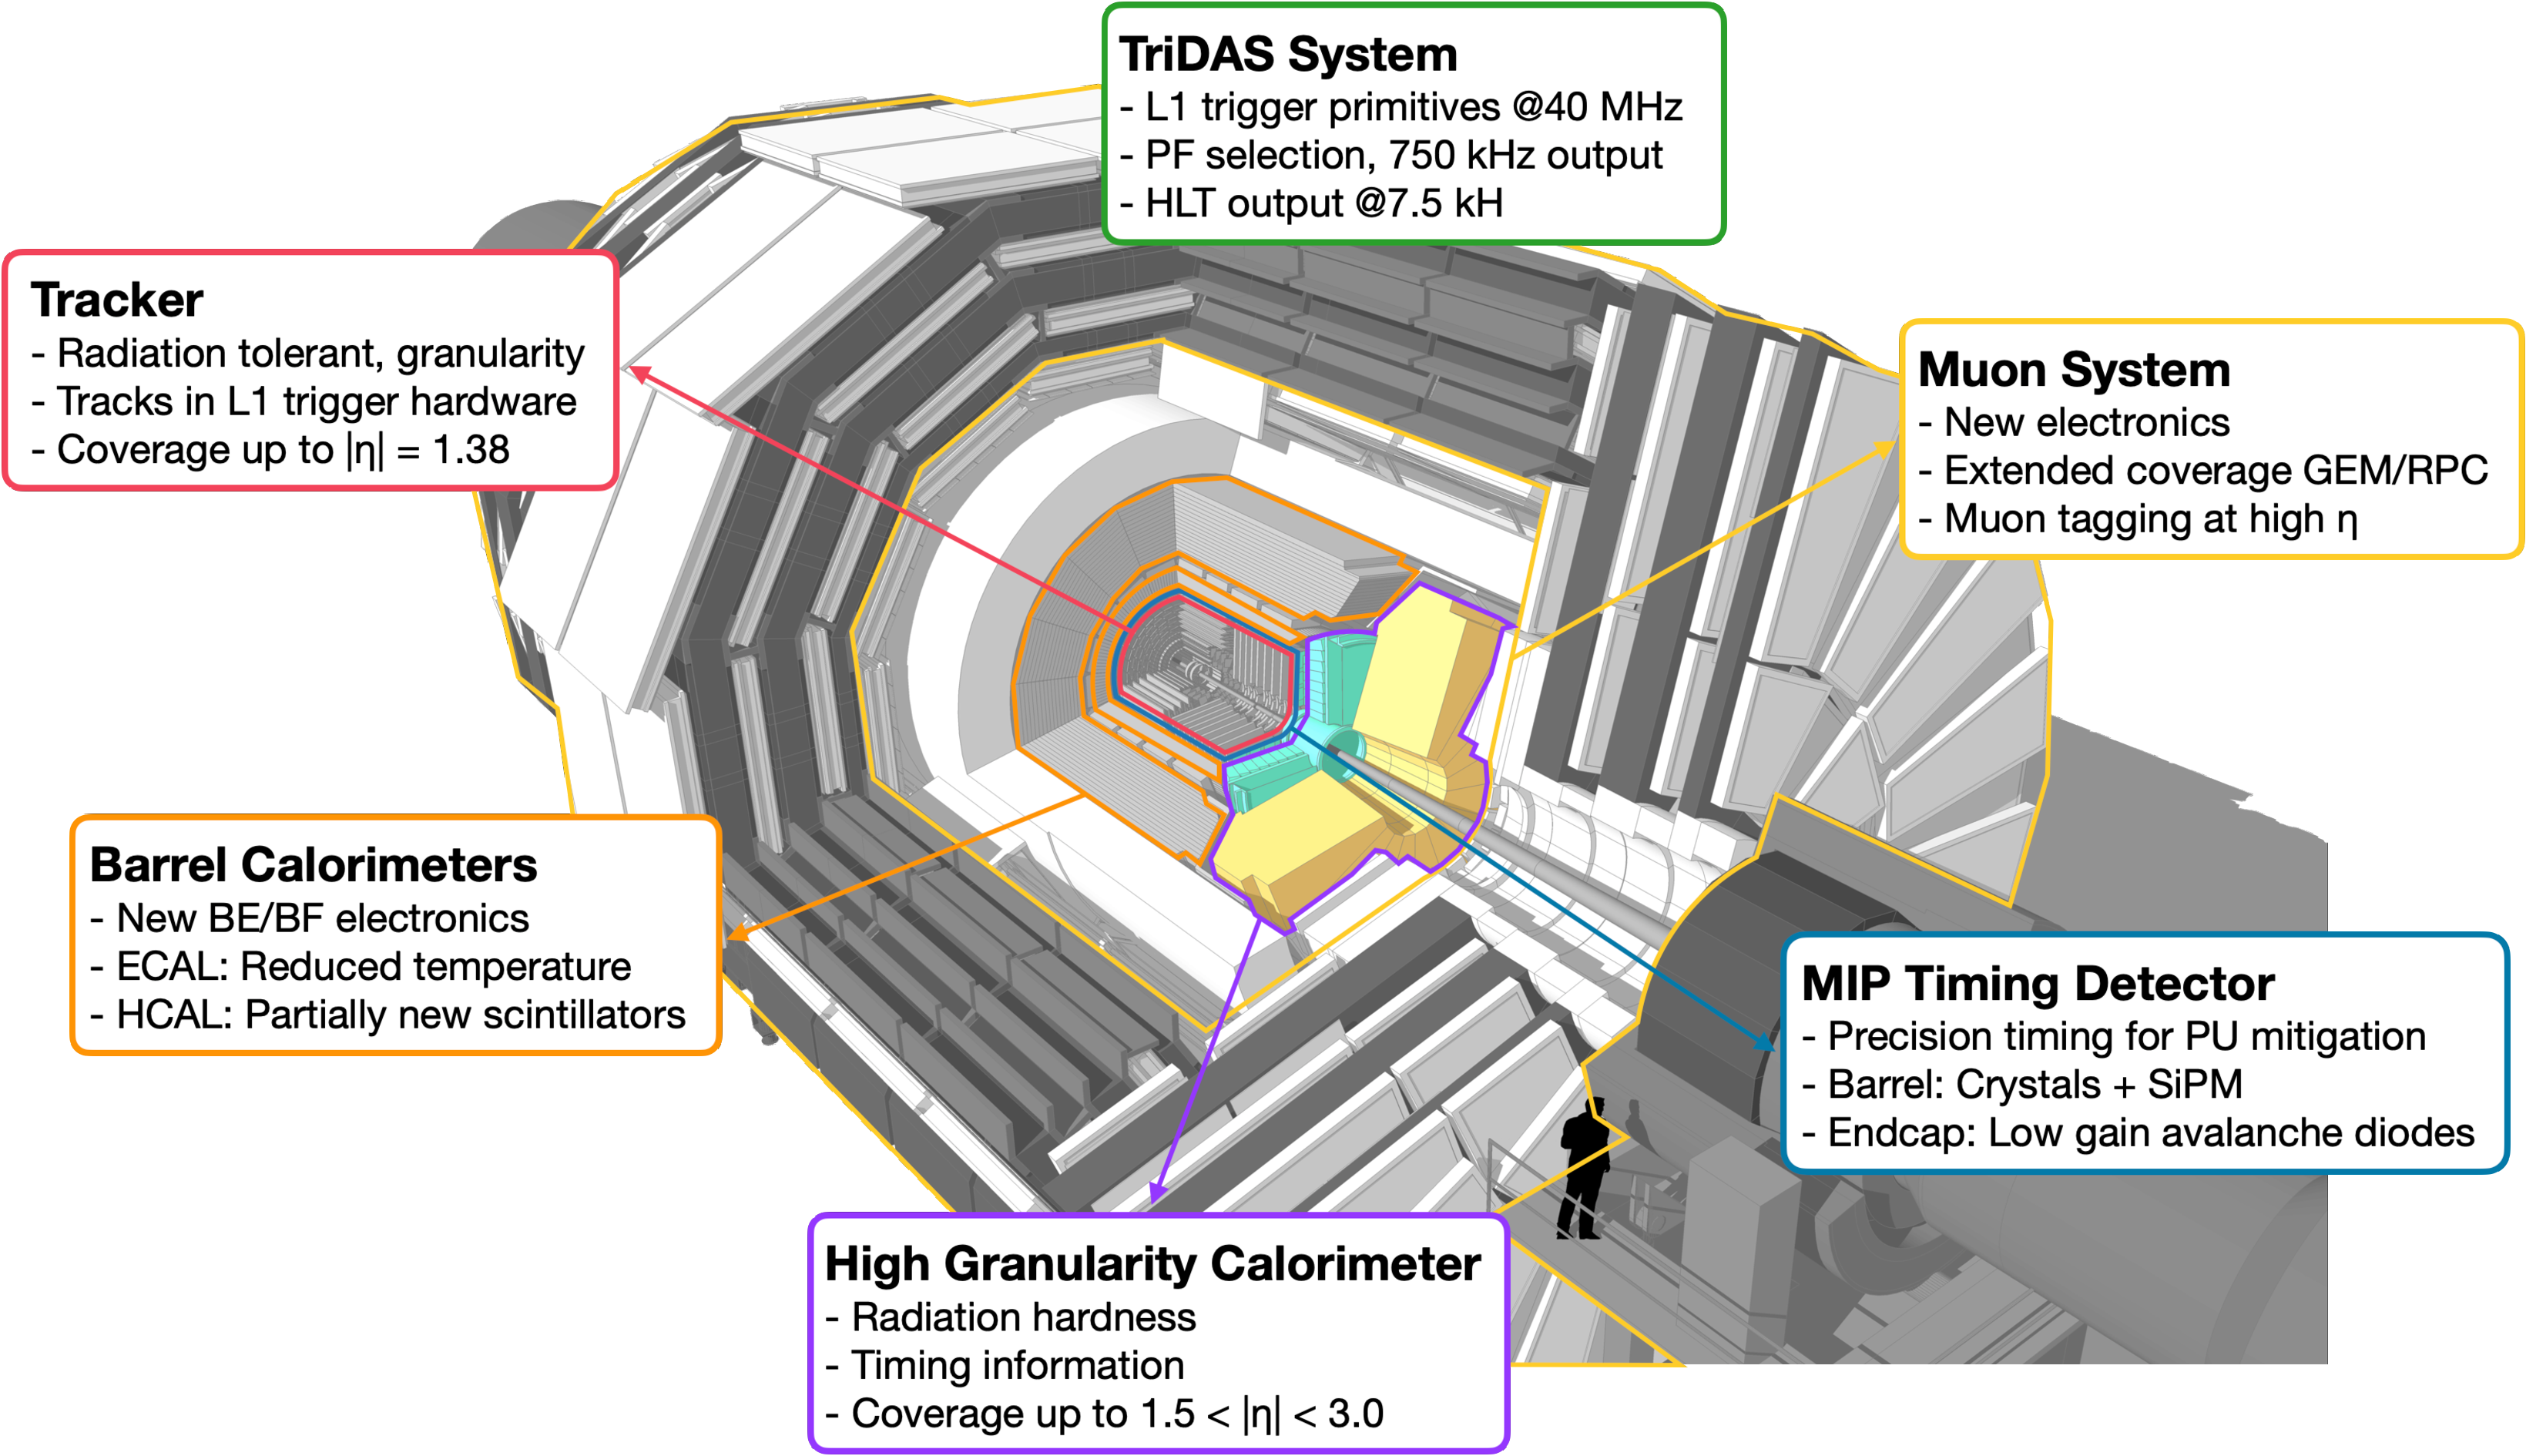
\includegraphics[width=0.95\linewidth]{Figures/HGCAL/CMSUpgrades.pdf}
    \caption{Cross section of the CMS detector with the indication of the upgrades foreseen for the HL-LHC.}
    \label{fig:CMSUpgrade}
\end{figure}

\section{The High-Granularity Calorimeter design}
\label{sec:The High-Granularity Calorimeter design}

Among the CMS detector updates, one of the most ambitious projects is the High Granularity Calorimeter (HGCAL), a high-granularity sampling calorimeter designed to replace the existing CMS endcap calorimeter in order to to maintain a excellent physics performance under the high pile-up and harsh radiation environment of the HL-LHC.

The existing $\textnormal{PbWO}_4$-based Endcap Calorimeters (CE) of the CMS detector were designed to sustain a total integrated luminosity of 500 $\textnormal{fb}^{-1}$. 
The transparency of the lead-tungstate crystals, already degraded during Run-II operations, would not survive the unprecedented radiation flux typical for the HL-LHC environment in this detector region.
It is therefore necessary to replace the current calorimeter endcaps with a new detector with high radiation tolerance, highly granular energy deposit and good time resolution to adequately treat pile-up in the offline event reconstruction. \newline

The HGCAL will consist of 47 layers divided into two compartments:
\begin{itemize}
    \item [-] the Electromagnetic Compartment (CE-E), featuring 26 active layers, interspersed with CuW, Cu, and Pb absorbers,
    \item [-] the Hadronic Compartment (CE-H), composed of 21 layers exploiting stainless steel as passive material.
\end{itemize}

The number of longitudinal samplings has been designed as a trade-off between the best shower reconstruction and the engineering requirements of the mechanical structure. 

To meet the radiation hardness requirements, the CE-E and the front part of the CE-H will employ silicon as active material, for a total area of about 600~$\textnormal{m}^2$ to be covered. In the remaining lower radiation regions of CE-H, at about 4~m from the interaction point, segmented plastic scintillators with silicon photomultipliers (SiPM) for the read-out will be used as the active material. Squared scintillator tiles with sizes ranging from 4~$\textnormal{cm}^2$ up to 30~$\textnormal{cm}^2$ will be installed, for a total of about 400~$\textnormal{m}^2$ of active area covered in scintillators.

This configuration amounts to a total of 10 nuclear radiation lengths ($\lambda_n$), divided into 1.3~$\lambda_n$ for the CE-E and 8.5~$\lambda_n$ for the CE-H. The CE-E alone will extend for a total of 27.7 radiation-lengths ($X_0$).
To further improve radiation resistance, the full system is cooled down to 240~K ($-30^{\circ}$C) with liquid $\textnormal{CO}_2$.

\begin{figure}
    \centering
    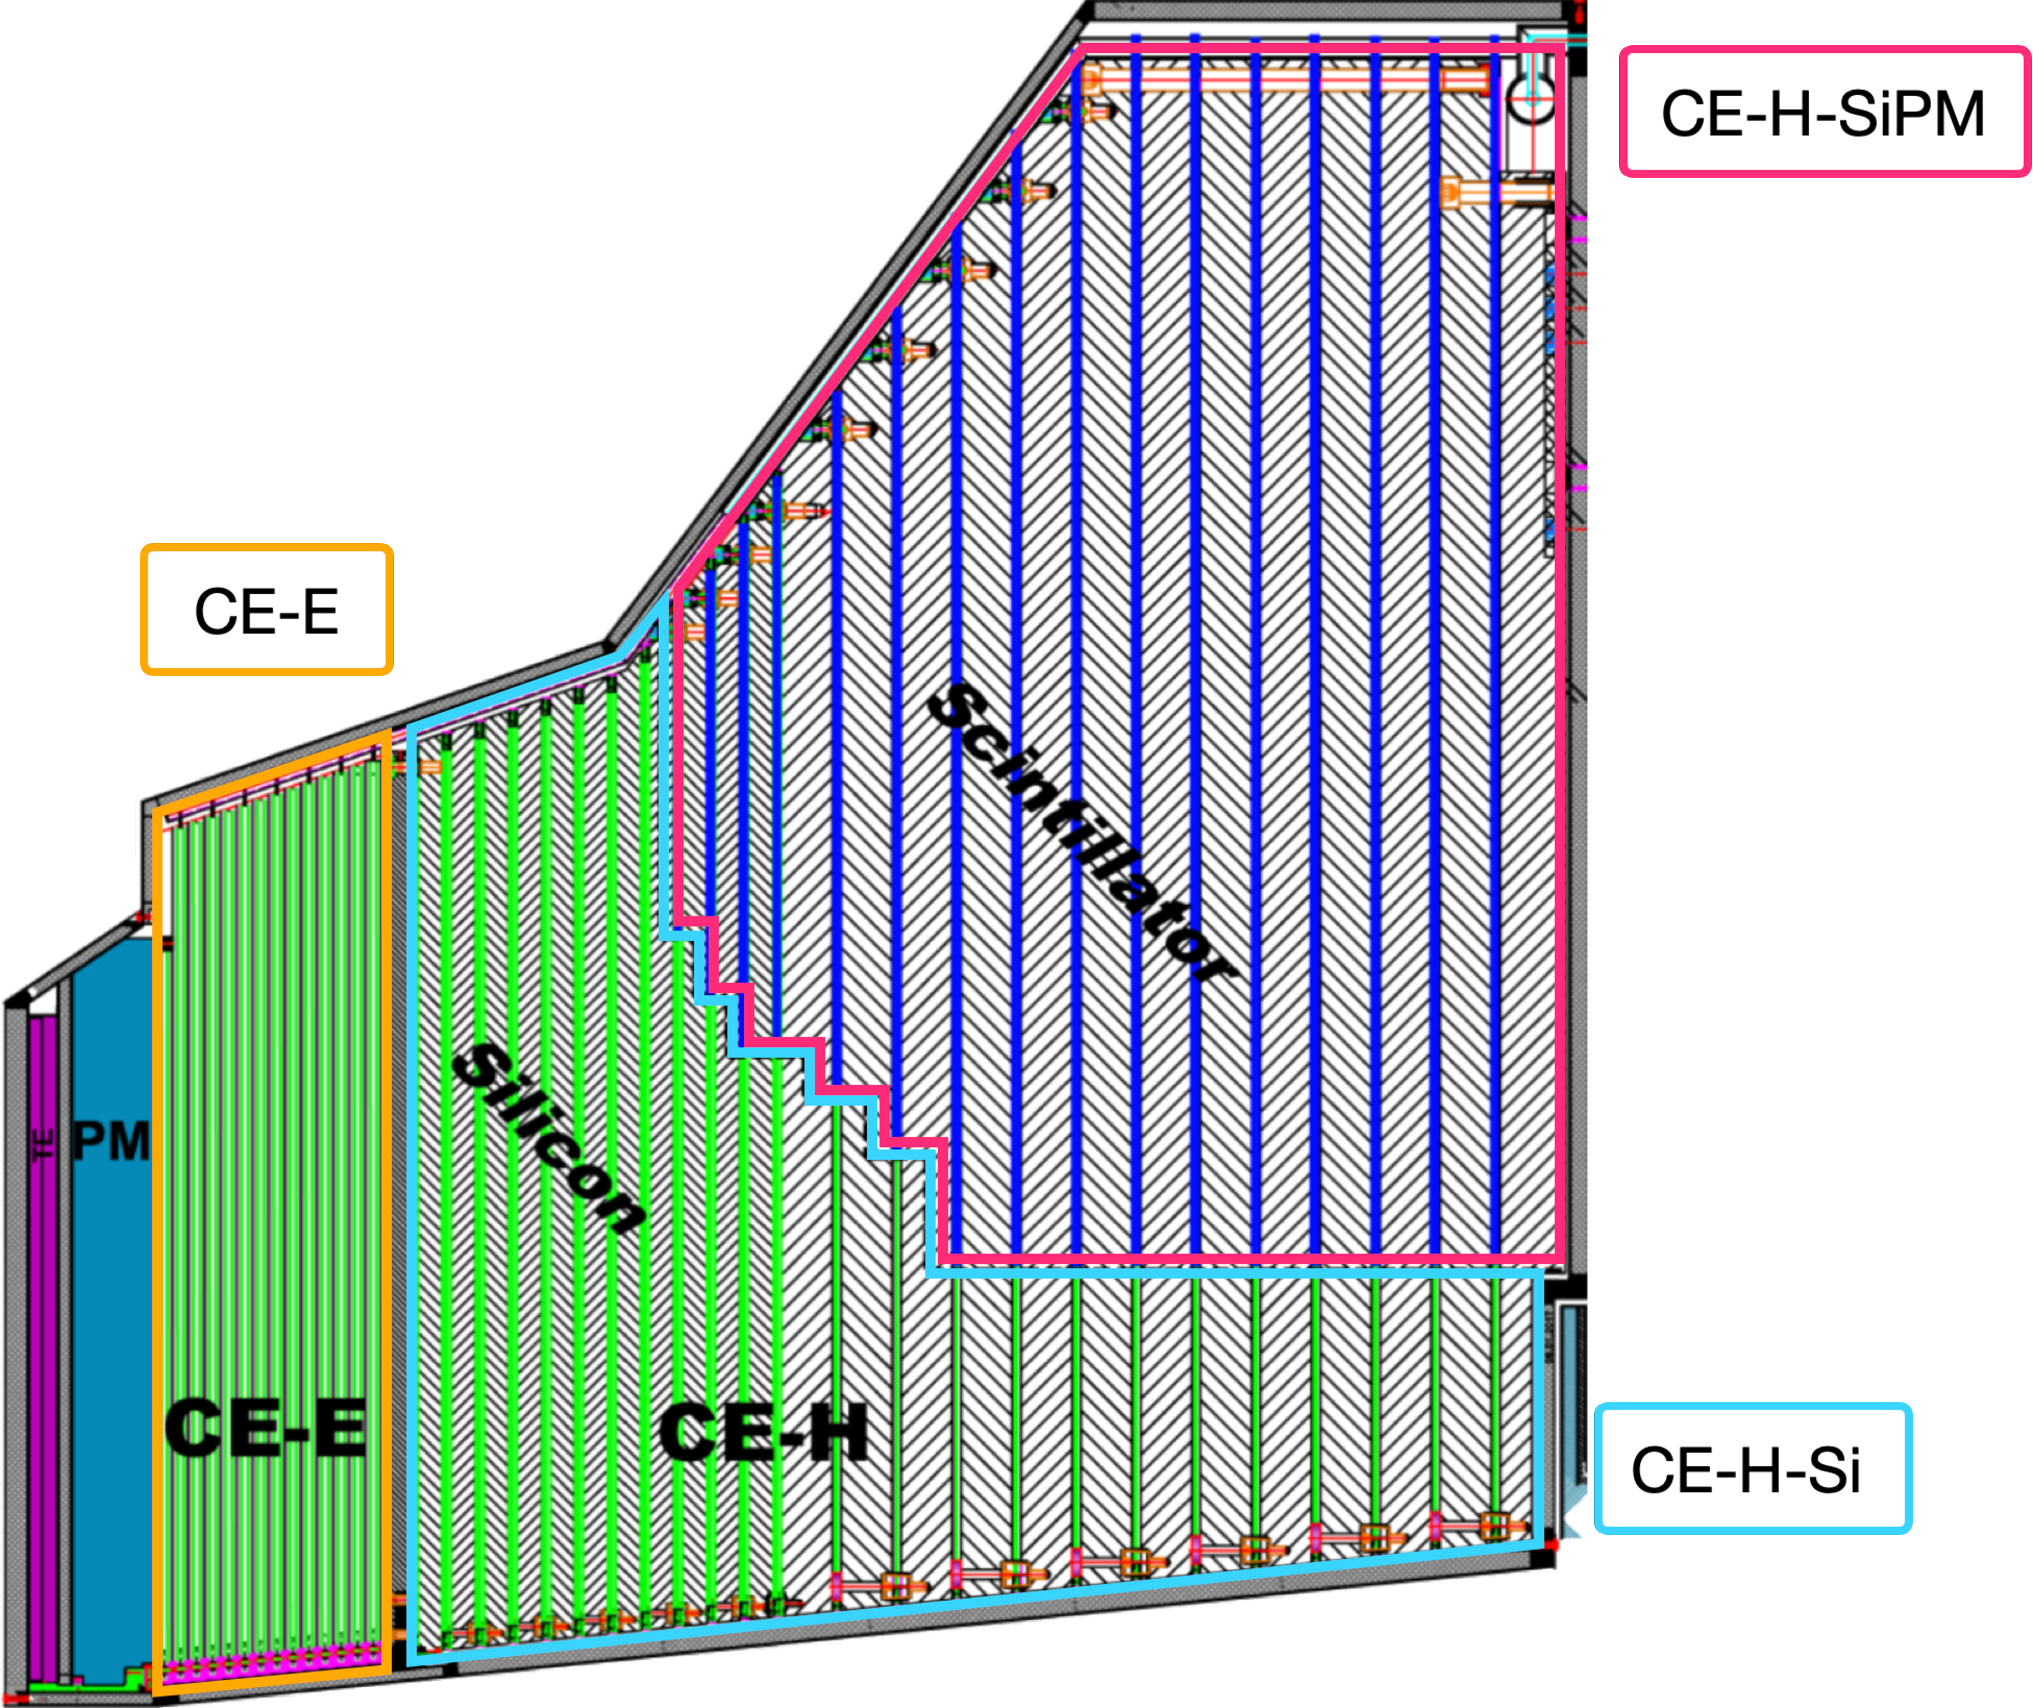
\includegraphics[width=0.6\linewidth]{Figures/HGCAL/HGCALLayers.pdf}
    \caption{Cross section view of the HGCAL. The CE-E and front CE-E compartments comprise silicon-based components. In its latest design, it features 47 layers divided into two regions: 26 silicon-based layers for the Electromagnetic Compartment (CE-E), 21 layers for the Hadronic Compartment (CE-H) using silicon (CE-H-Si) and scintillator-based (CE-H-SiPM) active material. The expected coverage of the HGCAL will range from $|\eta|=1.5$ up to $|\eta|=3.0$.}
    \label{fig:HGCALLayers}
\end{figure}

A longitudinal cross section of the HGCAL is shown in Fig.\ref{fig:HGCALLayers}, where the multiple layers if the Electromagnetic and Hadronic Compartments are visible, along with the different active material used in the two regions.

\bigbreak

In order to cover the area in the most cost-effective manner, the hexagonal geometry for the silicon sensors will be exploited. To reduce the number of modules, the baseline of the sensor size has been adjusted from the initially foreseen 6\mbox{''} design to 8\mbox{''}. An active thickness of 120, 200, or 300 $\mu$m is expected, depending on the detector region.
Each module will comprise several single read-out diodes, hereafter referred to as \textit{cells}, with a 0.5 or 1.0~$\textnormal{cm}^2$ active area, for a total of about six million cells to read out individually in the ultimate detector operation. 
The design, production, and validation of these hexagonal sensors, hereafter referred to as \textit{modules}, is one of the most challenging aspects of the HGCAL project. A more detailed discussion about silicon as active material and the structure of the HGCAL modules is given in Sec.~\ref{sec:Silicon Modules}. 

In the CE-E, the silicon modules will be used to create self-supporting sandwich structures which are commonly referred to as \textit{cassettes}. For this, the modules will be installed on both sides of a copper cooling plate and will be closed with lead plates.

In the low radiation CE-H-SiPM compartment, the scintillating material coupled to SiPMs read-out will be transversely segmented in square shapes with the size of 4 to 30~$\textnormal{cm}^2$, depending on the pseudorapidity position. 
The scintillator modules will be composed of tileboard printed circuit boards (PCBs) with different sizes and shapes. Each tileboard will host from 48 to 96 scintillator tiles individually wrapped into a reflecting layer and characterised by a cavity to contain the SiPM. Each detector on the board will be equipped with an ultraviolet LED next for the calibration and monitoring of the SiPM gain. 

This geometrical configuration amounts to a total active area of 620~$\textnormal{m}^2$ and 370~$\textnormal{m}^2$ for the CE-E and CE-H compartments respectively and provides a compact and cost-effective way to build the entire calorimeter at a reasonable cost while meeting the strict radiation requirements in the high pseudorapidity region.

\begin{figure}
    \centering
    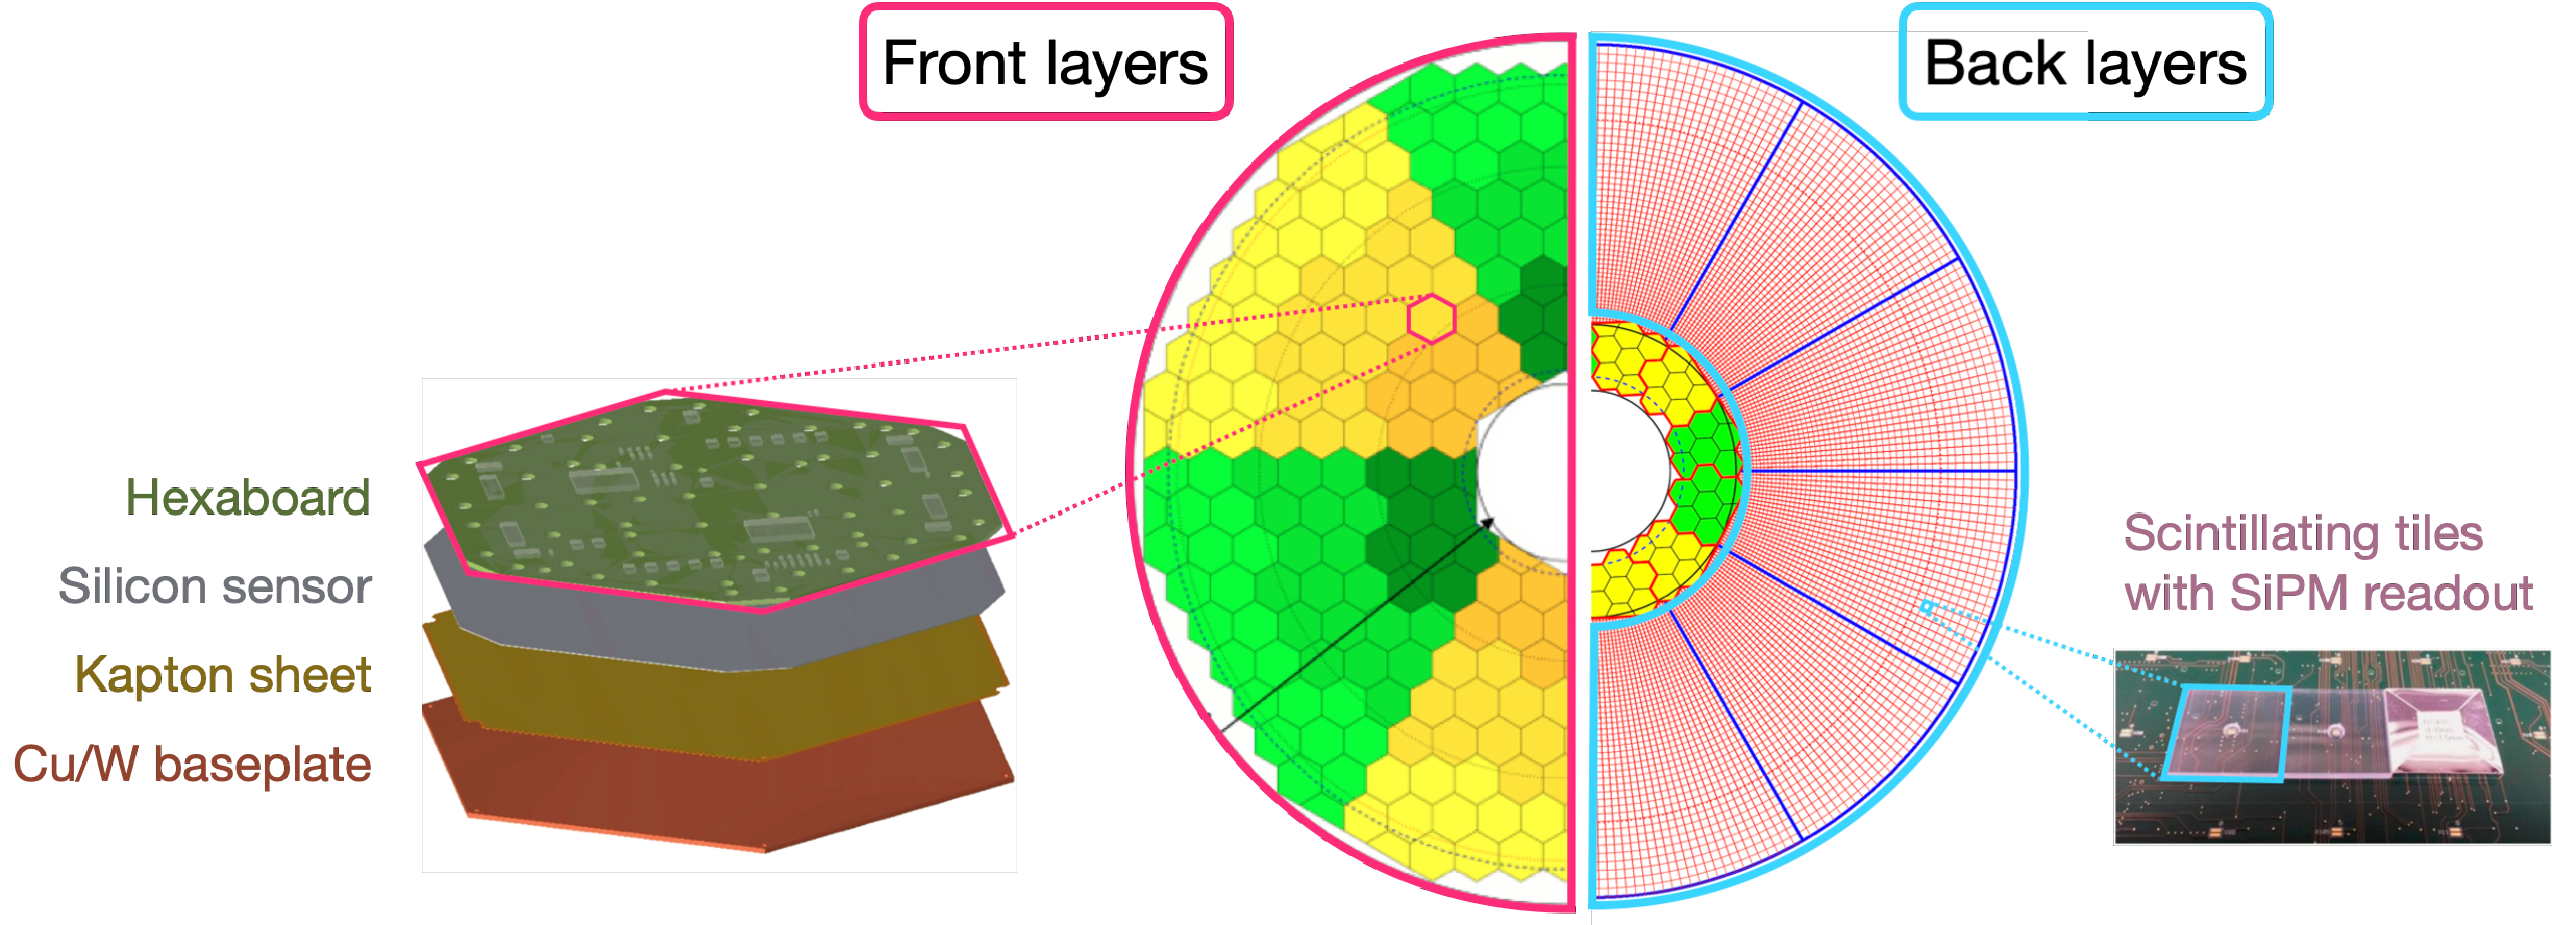
\includegraphics[width=0.9\linewidth]{Figures/HGCAL/FrontBackLayers.pdf}
    \caption{Schematic view of the arrangement of the hexagonal silicon modules in the front layers composing the CE-E and CE-H-Si (left) and of the scintillator tiles employed in the low radiation back layers of the CE-H-SiPM (right).}
    \label{fig:FrontBackLayers}
\end{figure}

The arrangement of the silicon modules in the CE-E and CE-H-Si (front layers) is represented in the left part of Fig.~\ref{fig:FrontBackLayers}, while the right part shows the scintillator tiles employed in the CE-H-SiPM region (back layers).

\bigbreak

The HGCAL design guarantees coverage in the pseudorapidity range $1.5 < |\eta| < 3.0$, featuring both highly granular lateral and longitudinal segmentation. 
The enhanced lateral granularity, combined with the dense absorbers, yields effective individual shower discrimination within the detector. Moreover, the finely segmented longitudinal structure enhances PU rejection, particle identification, and energy resolution. Because of these features, the HGCAL is often referred to as an \textit{imaging}, or 5D, calorimeter, the five dimensions corresponding to the three-dimensional spatial information provided by the fine voxels, the energy deposit in each active material segments, and the timing information with an expected resolution of $\mathcal{O}$(10 ps).

The calibration of the detector will be performed with minimum ionizing particles (MIP). To maintain a reasonable detection of MIPs over the detector's lifetime and ensure a signal-to-noise ratio above one, the effects of radiation damage must be minimized. To achieve this, the HGCAL will have to be operated at a constant temperature of -30~$^{\circ}$C or lower, obtained through a dedicated $\textnormal{CO}_2$ cooling system directly implemented in the copper base plate. 

\subsection{Silicon Modules}
\label{sec:Silicon Modules}

The choice of silicon as the active material in the HGCAL modules is driven by the stringent constraints imposed by the expected physics performance and operating conditions of the detector. 
Silicon sensors ensure the detection of minimum ionizing particles (MIPs) and facilitate precise measurement of high-energey showers, both crucial for the HGCAL's operation efficiency. The former is essential for \textit{in situ} calibrations of the detector, while the latter can be ensured only with a full containment of the showers, which relies on the detector compactness achieved through thin silicon modules and a proper mixture of absorbers.

These requirements are met by silicon sensors, which offer rapid signal response $\mathcal{O}$(10 ns) necessary to keep up with the expected 40 MHz rates at the HL-LHC. Additionally, silicon module production benefits from established large-scaled industrial capabilities, allowing for relatively short lead times.

The validation of the silicon modules structure has been cornerstone of the project since the approval of the HGCAL Technical Proposal (TP) in 2015. Several proof-of-concept modules, produced by Hamamatsu Photonics K.K. (HPK), have undergone extensive testing in beam experiments between 2016 and 2017. Insights from these tests, incorporated into the 2018 HGCAL Technical Design Report (TDR), form the foundation for understanding the properties of silicon modules crucial for such a complex detector.

\bigbreak

The HGCAL will require approximately $27\,000$ silicon detector modules to be assembled and installed in its electromagnetic (CE-E) section and part of the hadronic (CE-H) section.

Each module consists of stacked layers comprising the printed circuit board (PCB), labeled \textit{hexaboard}, where the front-end electronics are installed, a silicon sensor, and a gold-plated Kapton sheet providing HV connection to the sensor back-plane and electrical insulation. The baseplate, made of materials such as CuW or Cu, provides enough rigidity to support the module whilst minimizing the total radiation length and dissipating the heat through a dedicated cooling system.

The silicon modules will be further segmented into either 192, for low-density (LD), or 432 individual diodes, for high-density (HD) modules. The diodes will act as sensor cells and have a separate read-out channel.

\begin{figure}
    \centering
    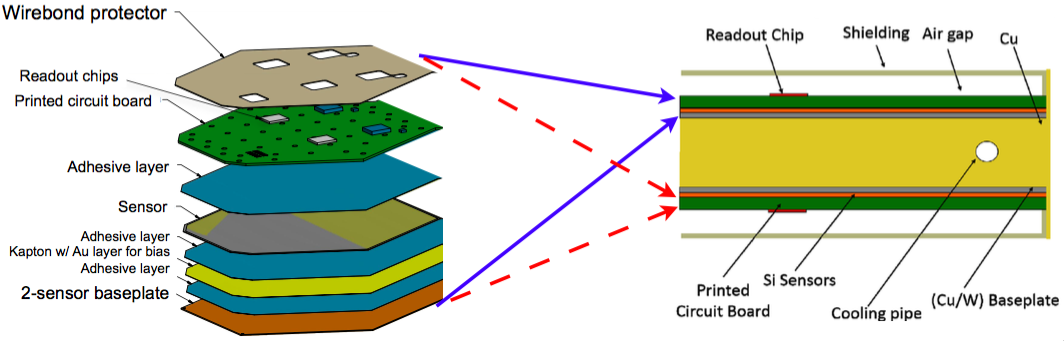
\includegraphics[width=0.9\linewidth]{Figures/HGCAL/ModuleDesign.png}
    \caption{Composition of a silicon module and placement in the copper plate. Each module is a stack of different layers, starting with a baseplate at the bottom, covered with a gold plated Kapton foil on which stands the silicon sensor. A protected PCB with read-out chip is placed on top.}
    \label{fig:ModuleDesign}
\end{figure}

A schematic view of the structure of a typical HGCAL module is given in Fig.~\ref{fig:ModuleDesign}.

\subsection{Plastic Scintillation Tiles}
\label{sec:Plastic Scintillation Tiles}

The remaining portion of the CE-H compartment will incorporate scintillator as the active material in regions where the integrated dose remains low-enough ($<3$~kGy) to maintain optimal performance throughout the entire lifespan of the HL-LHC. 
This approach will also ensure effective muon identification in the $\eta>2.4$ region, where muon chambers are not available.

The scintillator will be crafted into small squared tiles, with the scintillation light reflected by a wrapping foil and directly read-out by a SiPM optically coupled through a small \textit{dimple} in the centre of one face of each tile. The SiPMs will be mounted on printed circuit boards, matched to the appropriate tiles. 
The system is illustrated in Fig.\ref{fig:ScintillatorTiles}.

In conformity with the CMS endcap's geometry, the scintillator cells will be arranged in an $r,\phi$ grid. As a result, cells closer to the beam line will be significantly smaller (4~$\textnormal{cm}^2$) than those at the outer edge (32~$\textnormal{cm}^2$). 

The area instrumented with scintillator will be subdivided into tile-modules consisting of a tileboard and the scintillator tiles. These tile-modules will then be connected together to form a 10~$^{\circ}$ detector unit. Six such units will be placed next to each other and combined with silicon modules into cassettes, covering 60~$^{\circ}$ each. Finally, six cassettes will collectively complete the calorimeter layer around the beam pipe.

\begin{figure}
    \centering
    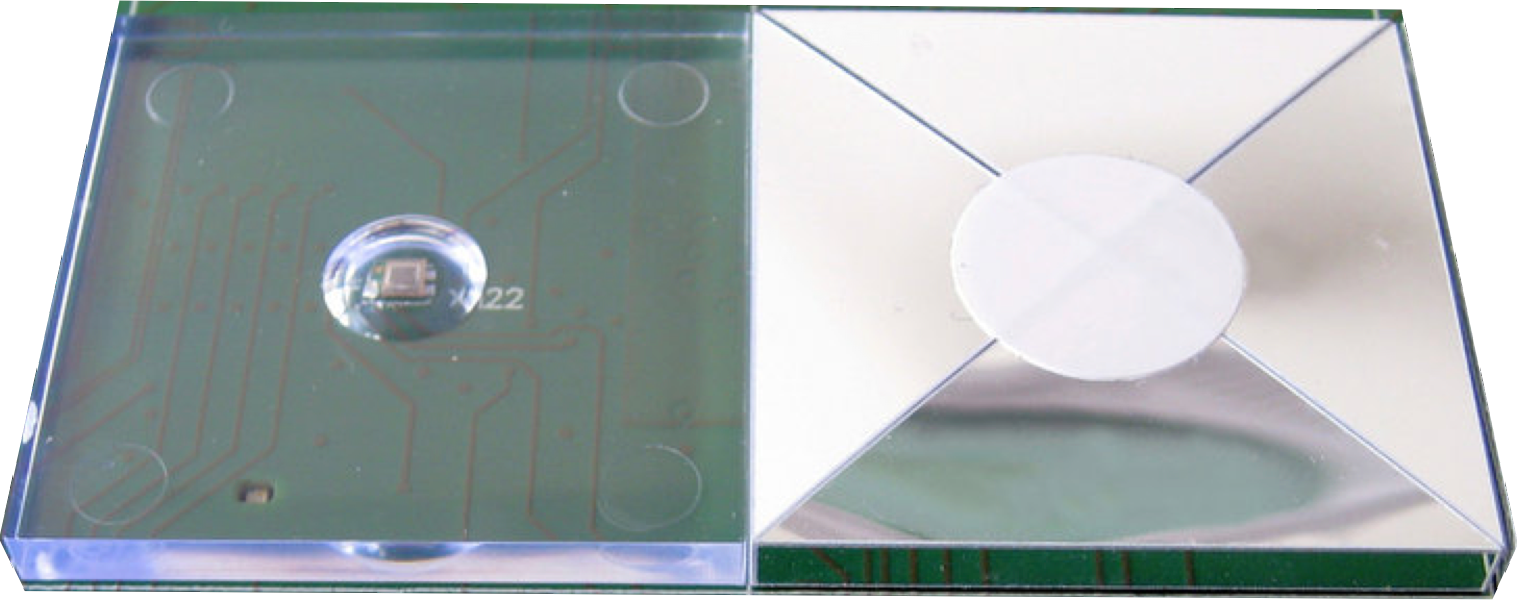
\includegraphics[width=0.5\linewidth]{Figures/HGCAL/ScintillatorTiles.pdf}
    \caption{Example of two $3\times3\textnormal{cm}^2$ scintillator tiles with a central dimple, unwrapped (left) and wrapped (right), mounted on a PCB housing one SiPM per tile, used as a prototype for the HGCAL project.}
    \label{fig:ScintillatorTiles}
\end{figure}

\section{The HGCAL Front-End Electronics}
\label{sec:The HGCAL Front-End Electronics}

One of the most challenging aspects in the design of the HGCAL silicon and scintillator modules is the front-end (FE) electronics. 

The FE electronics is responsible for several critical functions within the HGCAL system. It measures and digitizes the charge deposited in the silicon sensor pads or generated in the SiPMs, providing precise time measurements for the pulses. It transmits the digitized data to the back-end (BE) electronics located in the service cavern. It also computes, at each bunch crossing, the digital sums of neighboring cells, tailored to the specific cell sizes ($2\times2$ cells for 1~$\textnormal{cm}^2$ pads silicon sensors, 3 cells for 0.5~$\textnormal{cm}^2$ sensors, and 2 cells for scintillator tiles) to be transmitted to the trigger BE electronics to build trigger primitives.

Besides the unprecedented readout segmentation, the performance requirements for the FE electronics are extremely stringent, particularly for the silicon part of the detector:
\begin{itemize}
    \item [-] Low noise and large dynamic range, spanning from approximately 0.2~fC to 10~pC, equivalent to 16 bits. This range enables the detection of MIPs in the silicon sensors and recording of high-energy deposits from electromagnetic showers. 
    The electronics noise must be below 2000 electrons for a 65~pF capacitance pad to allow MIP visibility during the whole operation.
    \item [-] Integral linearity must exceed 1$\%$ across the entire dynamic range.
    \item [-] Timing information with a precision better than 100~ps for pulses above 12~fC, corresponding to about 3~MIPs in the 300~$\mu$m silicon sensors.
    \item [-] Fast shaping time (peaking-time $<20$~ns) to minimize the out-of-time pileup: the pulse should be dropped to less than 20$\%$ by the next bunch crossing.
    \item [-] On-detector digitization and data processing for zero suppression, linearization and summing of the trigger data.
    \item [-] Maximum latency of 36~bunch crossings for the trigger primitives at the output of the detector.
    \item [-] Buffering of the data to accommodate the 12.5~$\mu$ms latency of the L1 trigger.
    \item [-] High-speed read-out links to interface with the 10~Gb/s low-power GBT (LpGBT) serializer.
    \item [-] Low power budget ($<20$~mW per channel), typically limited by cooling power.
\end{itemize}

Following the LHC data-taking conditions, the acquisition chain must handle consecutive event arrivals at 40~MHz without data erasure.
Moreover, the FE electronics will face a harsh radiation environment which will reach 200~Mrad at the end of life and requires good radiation tolerance.

\begin{figure}
    \centering
    \includegraphics[width=0.95\linewidth]{Figures/HGCAL/Hexaboards.pdf}
    \caption{Plan view of two hexaboards housing 6 High Density (HD) HGCROC read-out chips: each chip is connected to 72 hexagonal cells. The connector will be used for the assemply of the motherboard, containing the ECON-D and ECON-T concentrator chips.}
    \label{fig:Hexaboards}
\end{figure}

\bigbreak

The very first step of the FE electronics read-out chain is the HGCal Read-Out Chip (HGCROC), which measures the charge and the time of arrival at 40~MHz frequency. The HGCROC is directly bonded through a ball-grid array to the hexaboard and has multiple channels connected to individual cells. 
The read-out chips, the linear voltage regulators (LVR), and any other passive and service components are mounted on a hexagonal module PCB, called \textit{hexaboard}, which is glued onto the silicon sensor. Imprinted on the hexaboard are also the pads for connections to the next board in the chain, labeled \textit{motherboard}. Through these connections also supply the LV, and the received and transmitted signals and data. 

\bigbreak

The next level of the FE electronics includes the concentrators, located on motherboards sitting 1.6~mm above the hexaboards. A motherboard serves from one to six modules, depending on the occupancy of the sensors. The surfaces which include the components of the hexaboard and of the motherboard face each other in order to reduce the overall thickness. 

The architecture of the very FE electronics chain on the hexaboards is summarised in Figure~\ref{fig:Hexaboards}. 

\section{The HGCROC3 architecture}
\label{sec:The HGCROC3 architecture}

With an extraordinary technical effort to meet all these requirements, the HGCROC3 is the final version of the ASIC specifically designed by the CMS Collaboration, in collaboration with the Omega Microelectronics Center at École Polytechnique, to read-out the modules of the future HGCAL. 
Two versions of the same readout architecture have been developed, for the silicon (Si) and the scintillator tiles (SiPM) sections, where the latter is obtained by only adding a current conveyor and adapting the preamplifier of the silicon variant.

\bigbreak

The main function of the HGCROC3 is to measure and digitize the charge deposit and provide high precision time information of the particles crossing the detector layers. It is also able to compute the energy sum of neighbouring cells in order to contribute to the Level-1 (L1) trigger decision. 
The chip features 78 channels, each consuming less than 15 mW power, and is designed in a radiation-hardened 130~nm CMOS technology. Among the channels, 72 serve as standard cell read-outs, 2 function as calibration cells read-out, and the remaining 4 channels are not connected to any sensor cells, serving for common-mode noise estimation. 

The layout is symmetrically divided into two parts, of \textit{halves}, as shown in Fig.~\ref{fig:TowHalves}.
In Fig.~\ref{fig:Architecture} a schematics of the inner architecture of the ASIC is presented: the structure and characteristics of each component are described in the following paragraphs.

\begin{figure}
    \centering
    \includegraphics[width=0.75\linewidth]{Figures/HGCAL/TwoHalves.pdf}
    \caption{Layout of the HGCROC3 ASIC: the chip is divided into two symmetrical parts. The voltage reference is positioned near the chip's edge, the ADC reference and TDC controls are located in the central region.}
    \label{fig:TowHalves}
\end{figure}

\paragraph{Data path}
The data path is the core of the chip, replicated for 72 channels of the full analog chain, 4 common mode channels for the coherent noise subtraction, and 2 calibration channels for the MIP calibration. This component extracts from the signal input charge three digitised quantities to be sent to the back-end electronics: the ADC for the charge measurement, the ToA (Time-of-Arrival) for the time measurement, and the ToT (Time-over-Threshold) for the charge measurement of saturated signals. 

The charge digitization is achieved by a 10-bit~ADC in the linear range of the preamplifier; when it saturates, a 12-bit Time-to-Digital Converter (TDC) with 50~ps binning over 200~ns range provides the charge information by measuring the ToT. The ToA digitization is carried out by a similar dedicated 10-bit TDC with 25~ps binning over 25~ns range.
The low-noise preamplifier gain can be adapted to different detector regions, where the MIP energy deposit can vary depending on the sensor thickness and irradiation condition.
Under HL-LHC conditions, certain regions of the detector may exhibit notably high occupancy rates, reaching up to 50$\%$ of fired cells per bunch crossing: it is thus important that the analog shaper drops the signal sample to less than 20$\%$ by the next bunch crossing to mitigate the out-of-time pile-up.

Beyond the analog performance, the chip embeds a large part of digital processing to manage the Data and the Trigger paths. A 512-depth DRAM (RAM1) is used as a circular memory to buffer the data to accommodate the 12.5~$\mu$s latency of the L1 trigger, and a 32-depth DRAM (RAM2) is used as a FIFO after the L1 selection.
Two 1.28~Gbps links are dedicated to send out the full event information of the selected bunch crossings after a L1 request.

\begin{figure}
    \centering
    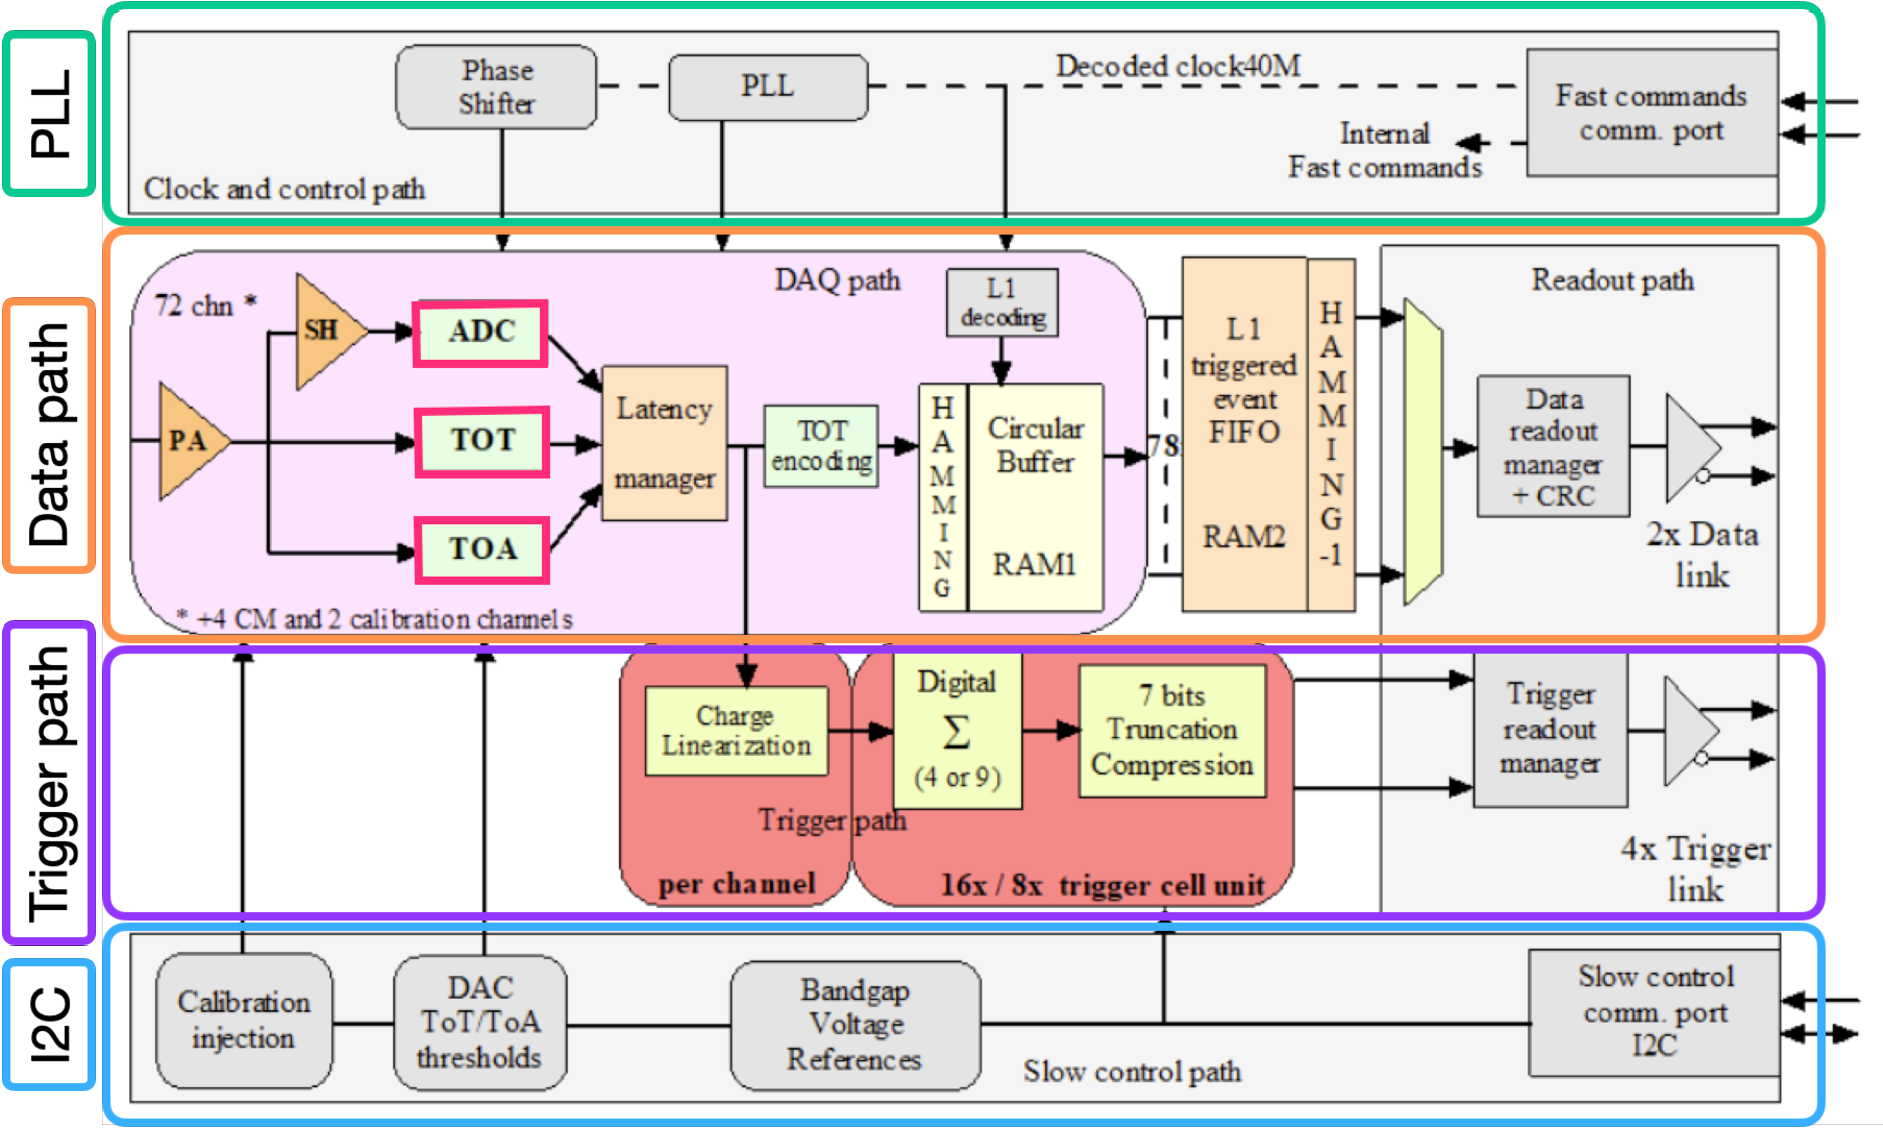
\includegraphics[width=0.75\linewidth]{Figures/HGCAL/Architecture.pdf}
    \caption{Architectural overview of the HGCROC3 read-out ASIC. The main parts composing the Data path, Trigger path, PLL and I2C have been highlighted.}
    \label{fig:Architecture}
\end{figure}

\paragraph{Trigger path}
The trigger path computes an image of the deposited charge at each bunch crossing, by summing and compressing data over neighbouring channels. The two charge-related quantities from the channel information (ADC and ToT) are fed into the trigger path. The chip performs the data processing with a charge linearisation over the ADC and ToT range and computes the energy sums over 4 (9) adjacent channels for the LD (HD) modules. After compressing the information to 7 bits, it sends the trigger data to the ECON-T concentrator chip.
Four $1.28\,\textrm{Gbps}$ differential links are devoted to send the energy sums for the L1 trigger decision. The data are sent to the ECON-T concentrator chip.

\paragraph{PLL}
The Phase-Locked Loop (PLL) is an analog clock synthesizer receiving the 40~MHz LHC clock and providing all the other clock frequencies - from 160~MHz to 1.28~GHz - used by the circuit.
The main challenge for the PLL circuit is to ensure that all the clocks' phases are aligned to the LHC 40~MHz input clock: a low noise digital Phase Frequency Detector (PFD) continuously checks for possible phase misalignments and, in case one is found, the chip adjusts the voltage-controlled oscillator (VCO) in order to temporarily increase or decrease the frequency and realign the phase. The PLL is an essential component for the HGCROC3 functioning and has been intensivley tested during the irradiation campaigns, as described in Sec.\ref{FIXME}.

\paragraph{I2C}
The Inter-Integrated Circuit (I2C) is an internal static memory register storing the chip's configuration parameters.
The I2C protocol is used to set or read the more than 7900 parameters, distributed into 8 internal registers.
A Fast Command block is used to read and write the configuration parameters, to configure the operating mode of the system (link synchronisation, reset, calibration, L1 request, etc.), and to communicate with the device.

\section{Characterisation and testing of the HGCROC3}
\label{sec:Characterisation and testing of the HGCROC3}

% Whe I arrived the new  HGCROC3 had just arrived and we had to test their performance in order to check whether the met the requirements
% What are the differences between HGCROC2 and 3?

	\chapter{The Calorimeter Layer-1 Trigger Primitives calibration}

\section{A novel Machine Learning method for detector objects calibration}
\label{sec:A novel Machine Learning method for detector objects calibration}

The energy calibration of calorimeters at collider experiments is of paramount importance for the physics performance.
Calorimeters are designed to measure the energy of high energy particles, such as photons and electrons producing electromagnetic showers, or quarks generating the hadronic showers due to color confinement and hadronisation. Whether it is a homogeneous calorimeter, capable of absorbing the energy of the particle shower in its entire depth, or a sampling calorimeter, where the energy is only detected in the active layers alternated to passive absorbers, calorimeters are hardly able to provide uniform response across the whole spatial and energy range. Calibration procedures are therefore fundamental to ensuring accurate energy measurement.

In order to improve spatial resolution in the reconstruction of the particles position, calorimeters can be segmented in the longitudinal and transverse directions, into ``calorimeter cells''. 
By clustering multiple cells together, it is possible to reconstruct the full shower energy deposit, whilst the spatial sampling can provide information about the particle position and, based on that, infer its four-momentum.
The essence of energy calibration consists of determining the optimal coefficients, known as calibration constants, that correct the individual cells energy, such that the energy of reconstructed particles aligns as closely as possible with their true energy. 
Several approaches exist to calibrate calorimeter cells.
For instance, in the case of the CMS electromagnetic calorimeter (ECAL), calibration constants are derived by either laser monitoring, i.e. using a laser a standard source of light to induce a response in the ECAL cells (lead-tungsten scintillating crystals), or by physics events such as photons from $\pi^0$ or $\eta$ meson decays, or electrons from $W$ or $Z$-boson decays~\cite{Cavallari:2798128}. These methods provide essential insights into the response of calorimeter cells, ensuring accurate energy reconstructions, crucial for precise particle physics measurements.

This chapter explores a novel machine learning approach tailored to effectively calibrate calorimeter objects by using higher-level and better-calibrated physics objects as a reference, such as the offline reconstructed particle energy.
The main advantage of the method is the possibility of calibrating CMS sub-detectors directly using data from proton-proton collisions or from test beams. This possibility is particularly beneficial when Monte Carlo simulations are not entirely reliable or not available.
Moreover, the method is particularly convenient when the number of cells is extremely high, such as for the future High Granularity Calorimeter (HGCAL), due to the scalability of ML methods and to the capabilities in treating and learning from a large number of input data simultaneously.

A proof of concept of the method has been implemented in the context of the Layer-1 Calorimeter Trigger Primitives calibration, where the number of parameters and the complexity of the trigger information are reduced. However, the performance of the method provides an improvement in the energy resolution that can be highly beneficial for the L1 Trigger efficiency.

% The technique uses Machine Learning to derive a set of calibration constants, optimized such that the sum of the calibrated cells energy approaches the energy of the corresponding reference object. In particular, I have played a major role in the first application of this technique, which was the calibration of the calorimeter trigger tower at Level-1 Trigger. In this context, the calibration constants depend on the trigger tower raw energy and position, and the algorithm targets the energy of the matched offline reconstructed electron or jet. We implemented the optimization algorithm using differentiable programming with the JAX Python library, which allows for the definition of custom losses and a fully configurable minimization. As one of the main project developers, I have also actively contributed to the the simulation and study of the input data, the hyperparameter optimization and the performance evaluation on electron and jet datasets. The corresponding set of scale factors will soon be deployed online. It is expected that the technique will also be employed in other contexts going forward, for example in the calibration of HGCAL cells."


\section{The calibration method applied to the Level-1 trigger}
\label{sec:The calibration method applied to the Level-1 trigger}

The CMS L1 Trigger system provides an optimal playground for testing the novel calibration approach, with the aim of improving the energy resolution of the trigger objects and providing a more efficient event selection.
The function of the L1 Trigger consists in combining the data coming from the CMS sub-detectors, detecting the potential presence of high energy objects or other interesting event features, to decide whether to accept or discard a given collision event. The role of the L1 Trigger system is essential to reduce the LHC collision rate of 40~MHz to only 100~kHz, the maximum data streaming rate reachable by the CMS data taking system.
The decision-making needs to occur within the 3.8~$\mu$s available latency, for this reason, the L1 decision cannot be based on the full event information, but on low resolution physics objects that only rely on the inputs coming from the calorimeters and the muon system, called \textit{L1 candidates}.
The input to the L1 Trigger is the so-called \textit{Trigger Primitives} (TPs), which are either produced by on-detector electronics placed in the experimental cavern, or by off-detector electronics in the service cavern. The TPs offer a coarse view of the physics event and can be combined together for the L1 object candidates. 

To operate a decision, the L1 trigger collects the information from the calorimeters and from the muon detectors separately. The object definition is run independently in the two sub-systems and combined at the final step by the Global Trigger algorithm, which performs the event accept or reject decision based on the L1 candidates kinematics and high-level variables, such as invariant masses and angular distances.

For this work, only the Calorimeter Trigger system has been considered for the application of the calibration method. In the calorimeter system, the information of the energy deposit in the HCAL and ECAL sub-detectors is processed by two consecutive systems, called respectively \textit{Layer-1} and \textit{Layer-2}. In the Layer-1 system, the TPs are calibrated and pre-processed before being sent to Layer-2 for object reconstruction. Given the stacked architecture of the two systems, better-calibrated objects at the output of the Layer-1 system can lead to significant improvement in the performance of the Layer-2 object definition, which would propagate in a more effective L1 Trigger decision.
The novel ML-based calibration method has been consequently applied to the calibration procedure of the Layer-1 calorimeter Trigger Primitives.
% One important example of how a lower- level calibration can largely benefit high-level objects is the PF algorithm; in this approach, the proper calibration of the PF elements ensures that the final PF candidates are well calibrated, and their high-level calibration factors are generally close to unity. For this reason, as part of this Thesis work, I have been the leading contributor to developing a novel technique for calibrating calorimeter TPs. This method is based on a ML approach and exploits offline reconstructed electrons and jets to calibrate single TPs optimally. This ML technique is detailed in the present Section; first, a brief overview of the past approach to TP calibration is given, highlighting its critical points, then the new method is described in detail, followed by the presentation of its performance.

\subsection{The Layer-1 calorimeter inputs}
\label{subsec:The Layer-1 calorimeter inputs}

The information from the ECAL, HCAL, and Hadron Forward (HF) detectors are transmitted to the L1 trigger system in the form of TPs, which are digital quantities corresponding to the 40~MHz samplings of the calorimeter pulses. Each sub-detector TP reflects the localised energy deposit in a specific sub-detector region, corresponding to an extension of $\Delta\eta\times\Delta\phi = 0.087 \times 0.087$ in the barrel: for ECAL each TP covers a square of $5\times5$ grid of crystals, while for HCAL it is equivalent to a single read-out unit.
Each half barrel of the CMS detector is consequently divided into 17 TPs along the $\eta$ direction, and into 72 TPs along the $\phi$ direction. Therefore, a discrete Trigger Tower two-indices Cartesian notation is employed to identify each TP using the pair ($i\eta$, $i\phi$). In this configuration, the TPs in the barrel have $i\eta$ and $i\phi$ indices such that $i\eta \in [-17,17] \setminus \{0\}$ and $i\phi \in [1,72]$, excluding position 0 from both directions.

A more complex definition of the TPs is required for the endcaps and HF, due to the varied geometry of the detector components.
In the ECAL endcap, where crystals are arranged in the specific pattern represented in Figure~\ref{fig:EE_HF_L1TP}~(a), to allow for a detailed analysis of the lateral energy spread of electromagnetic showers. In this region, the TPs do not follow exact ($\eta$, $\phi$) boundaries, but are defined in such a way that their extension in the $\eta$ dimension decreases radially as they approach the beam pipe. The resulting number of crystals in each TP varies from 25 for $|\eta|\sim1.5$ to 10 for $|\eta|\sim2.8$. 
This geometry is mainly designed to align with the HCAL tower geometry while maintaining a uniform segmentation of the detector.
In the HCAL endcap, each physical tower, which has an extension of $\Delta\phi = 0.174$, is evenly split into two TPs of $\Delta\phi = 0.087$. 
In this setup, the TPs in the endcap have $i\eta$ and $i\phi$ indices such that $|i\eta| \in [18,28]$ and $i\phi \in [1,72]$. 

For the HF detector, the same $\phi$-splitting geometry as the HCAL endcap is used, while the $\eta$ direction is divided into 12 segments, giving $|i\eta| \in [29,41]$ and $i\phi \in [1,72]$, as illustrated in Figure~\ref{fig:EE_HF_L1TP}~(b).

The CMS calorimeter trigger system has a total of 4,176 towers distributed in: 
\begin{itemize}
    \item 2,448 TPs in the ECAL and HCAL barrel,
    \item 1,584 in the ECAL and HCAL endcap,
    \item 144 in the HF calorimeter.
\end{itemize}
Figure~\ref{fig:Layer1} provides a schematic representation of the TP geometry. 

\begin{figure}
    \centering
    \subfloat[]{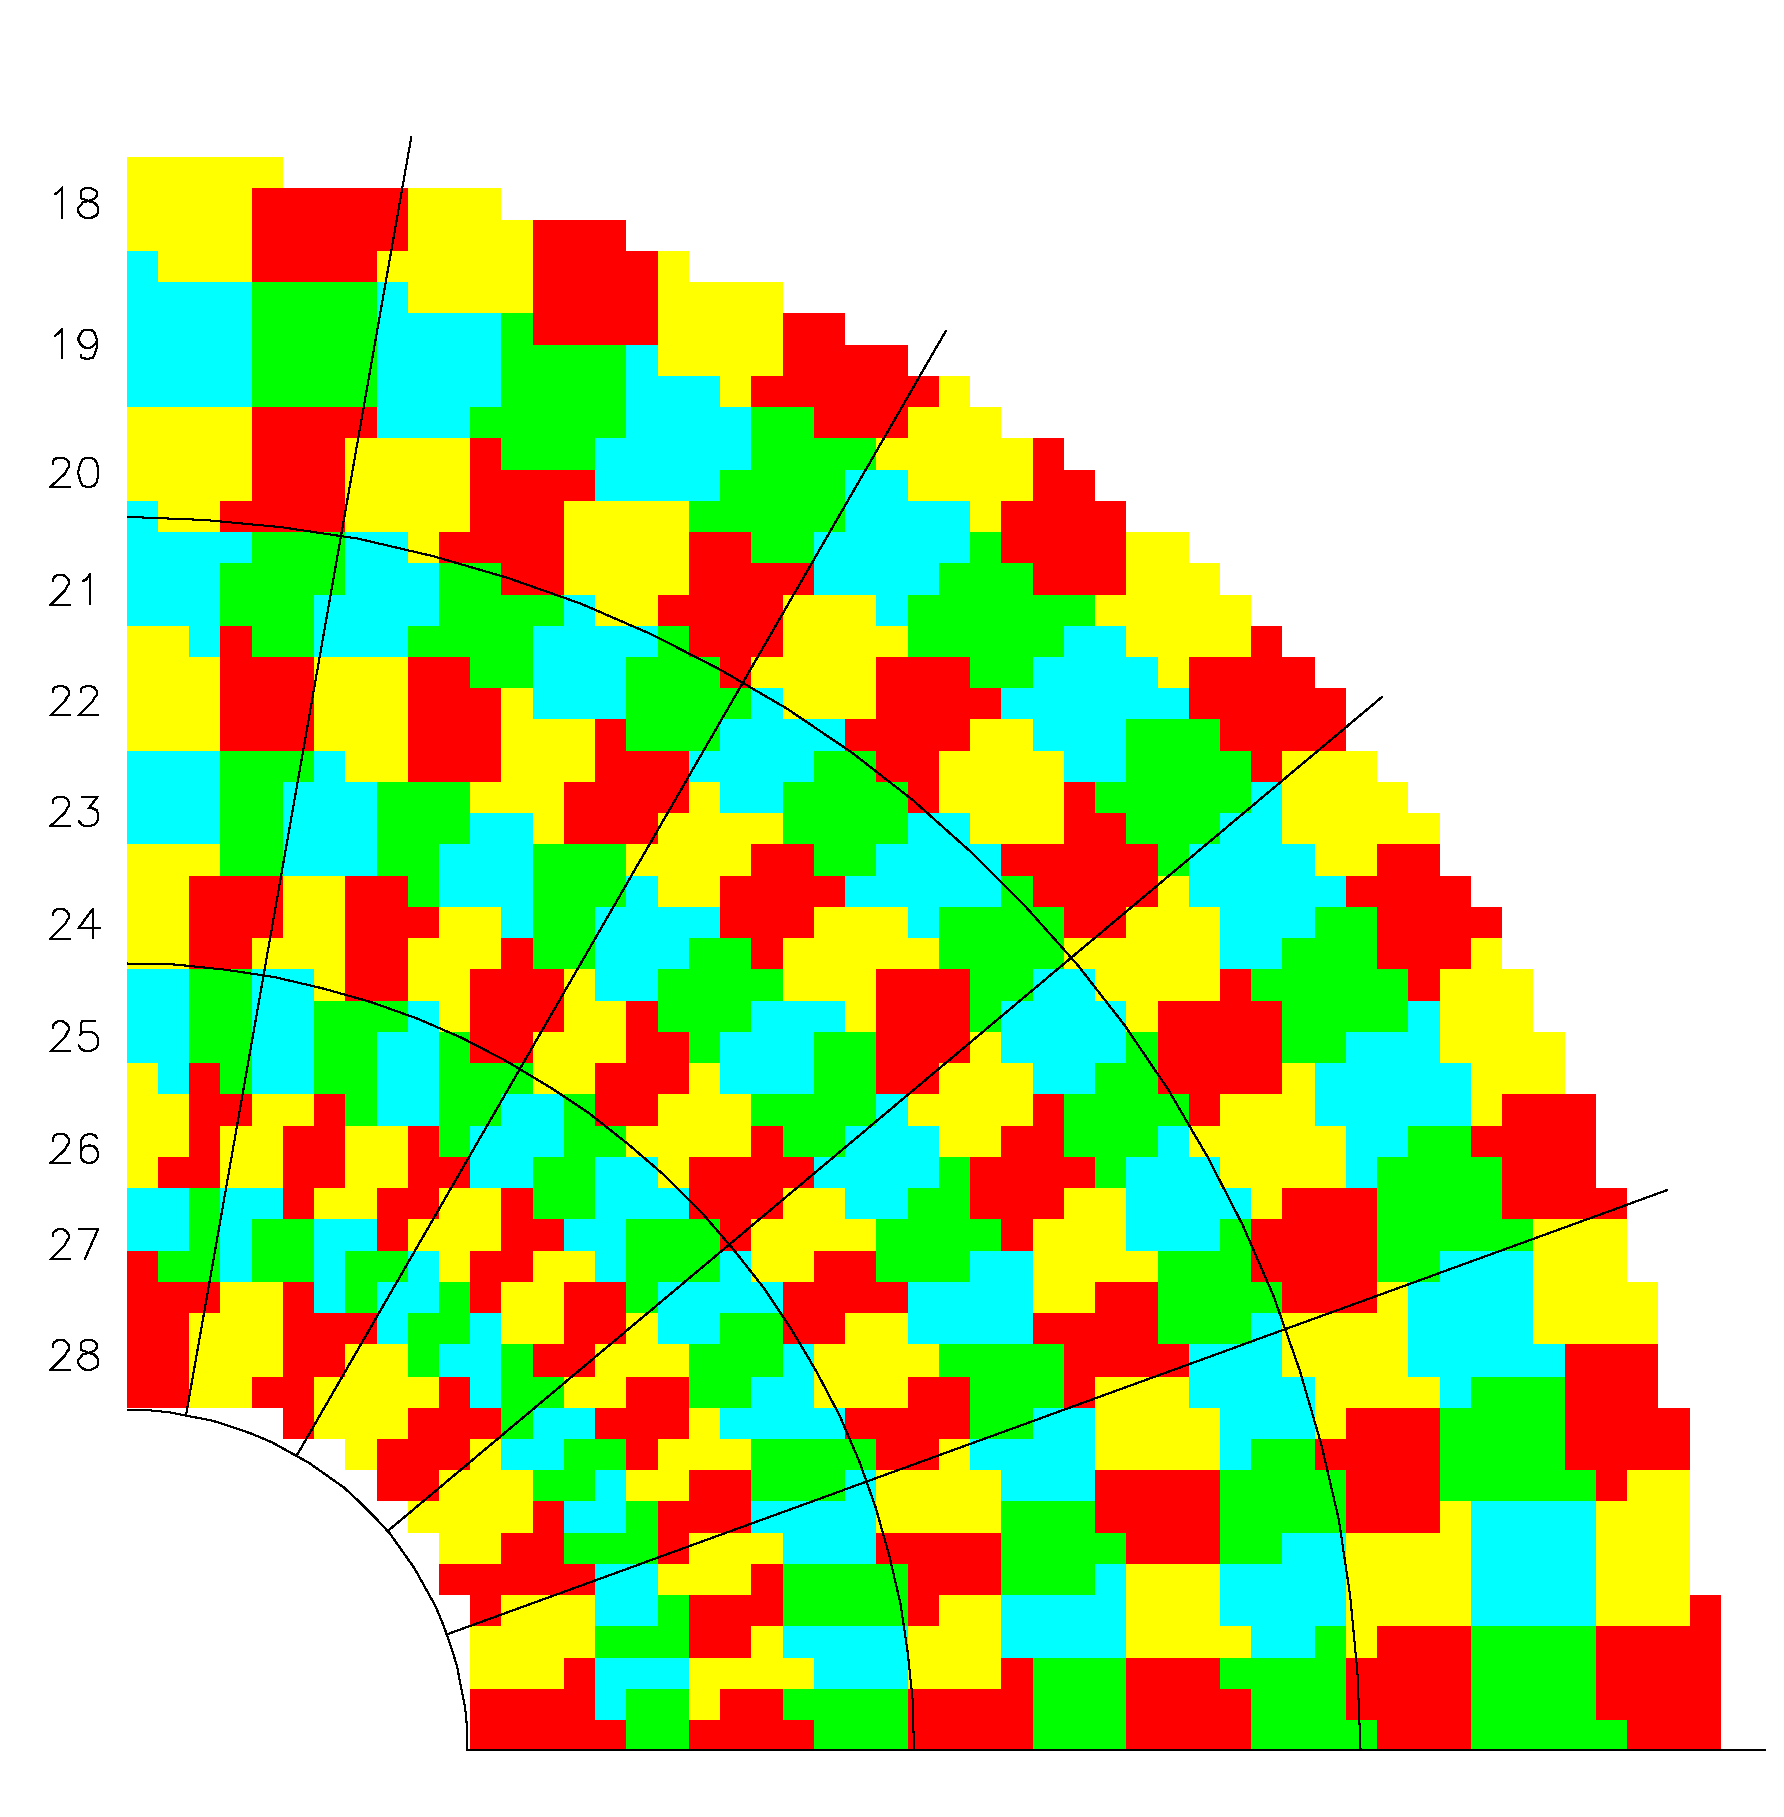
\includegraphics[width=0.4\linewidth]{Figures/L1TP/EE_L1TP.pdf}}
    \subfloat[]{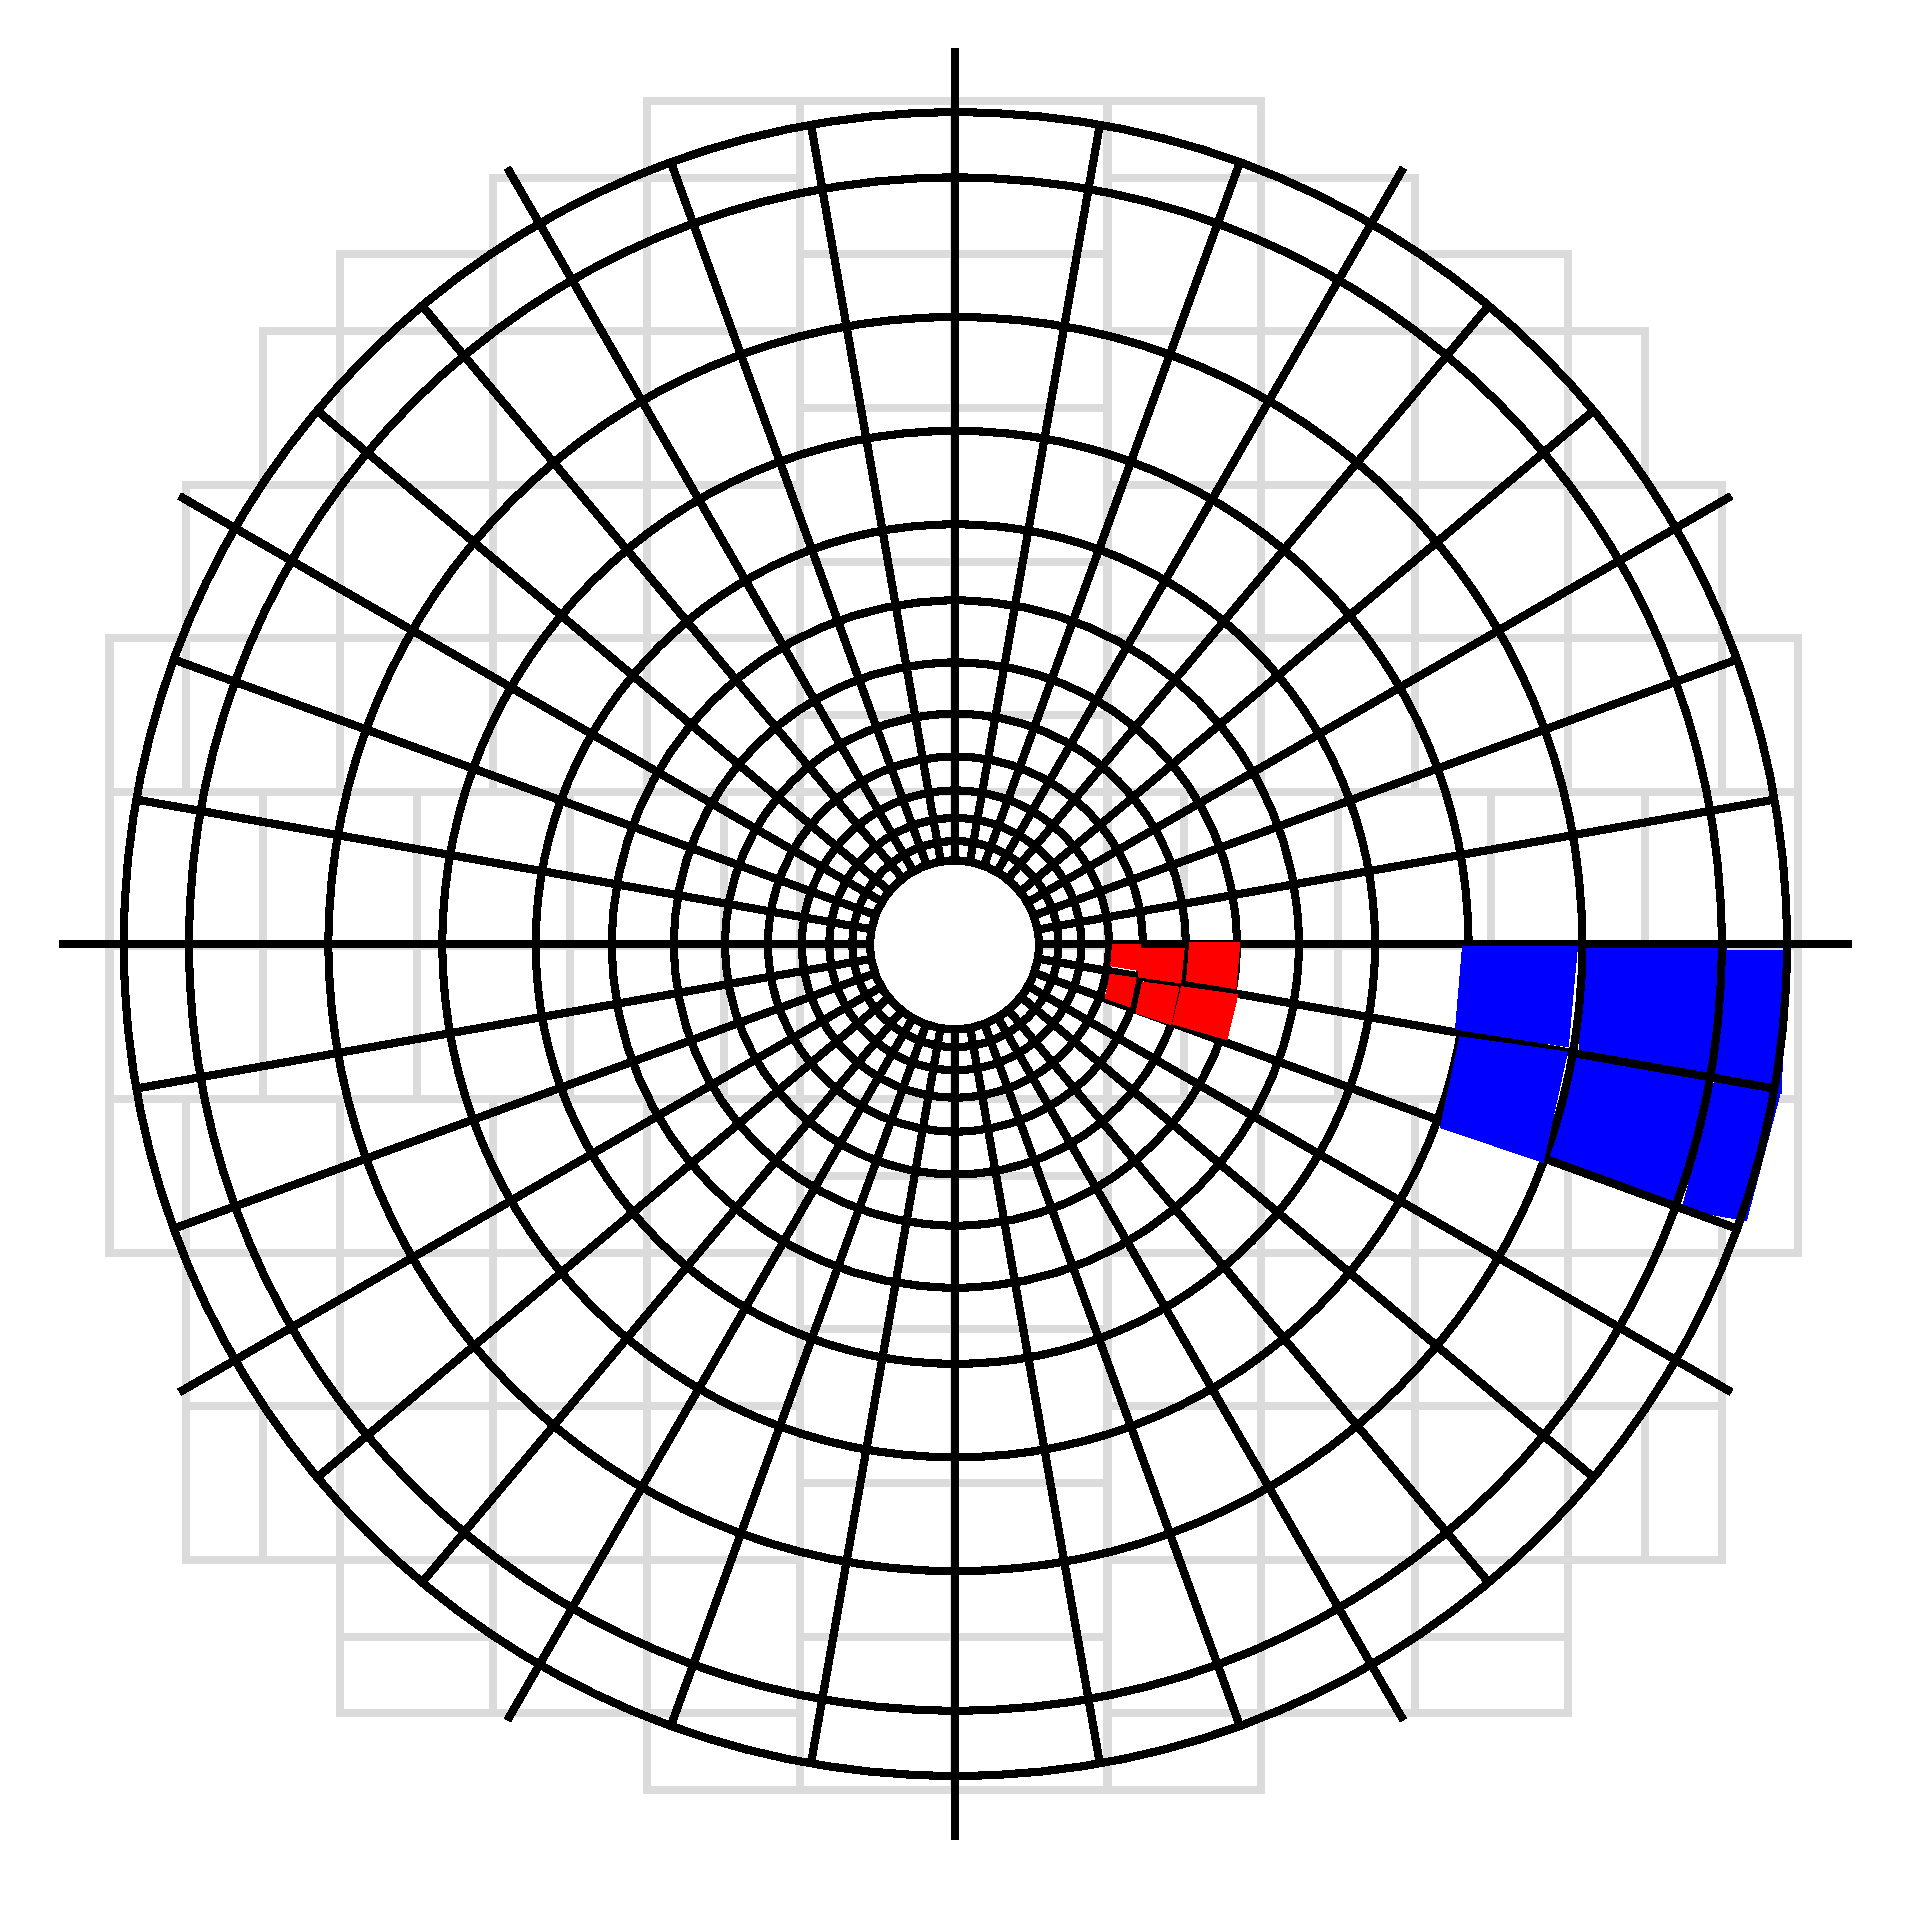
\includegraphics[width=0.4\linewidth]{Figures/L1TP/HF_L1TP.pdf}}
    \caption{Calorimeter Trigger Primitives (TP) layout in the x–y projection of the ECAL endcap (a); each square denotes a different ECAL crystal, and regions characterised by the same color represent one TP.
    Calorimeter TPs layout in the x–y projection of the HF detector (b); each square denotes a HF read-out unit, and regions with the same colour represent one Trigger Tower (TT).}
    \label{fig:EE_HF_L1TP}
\end{figure}

\begin{figure}
    \centering
    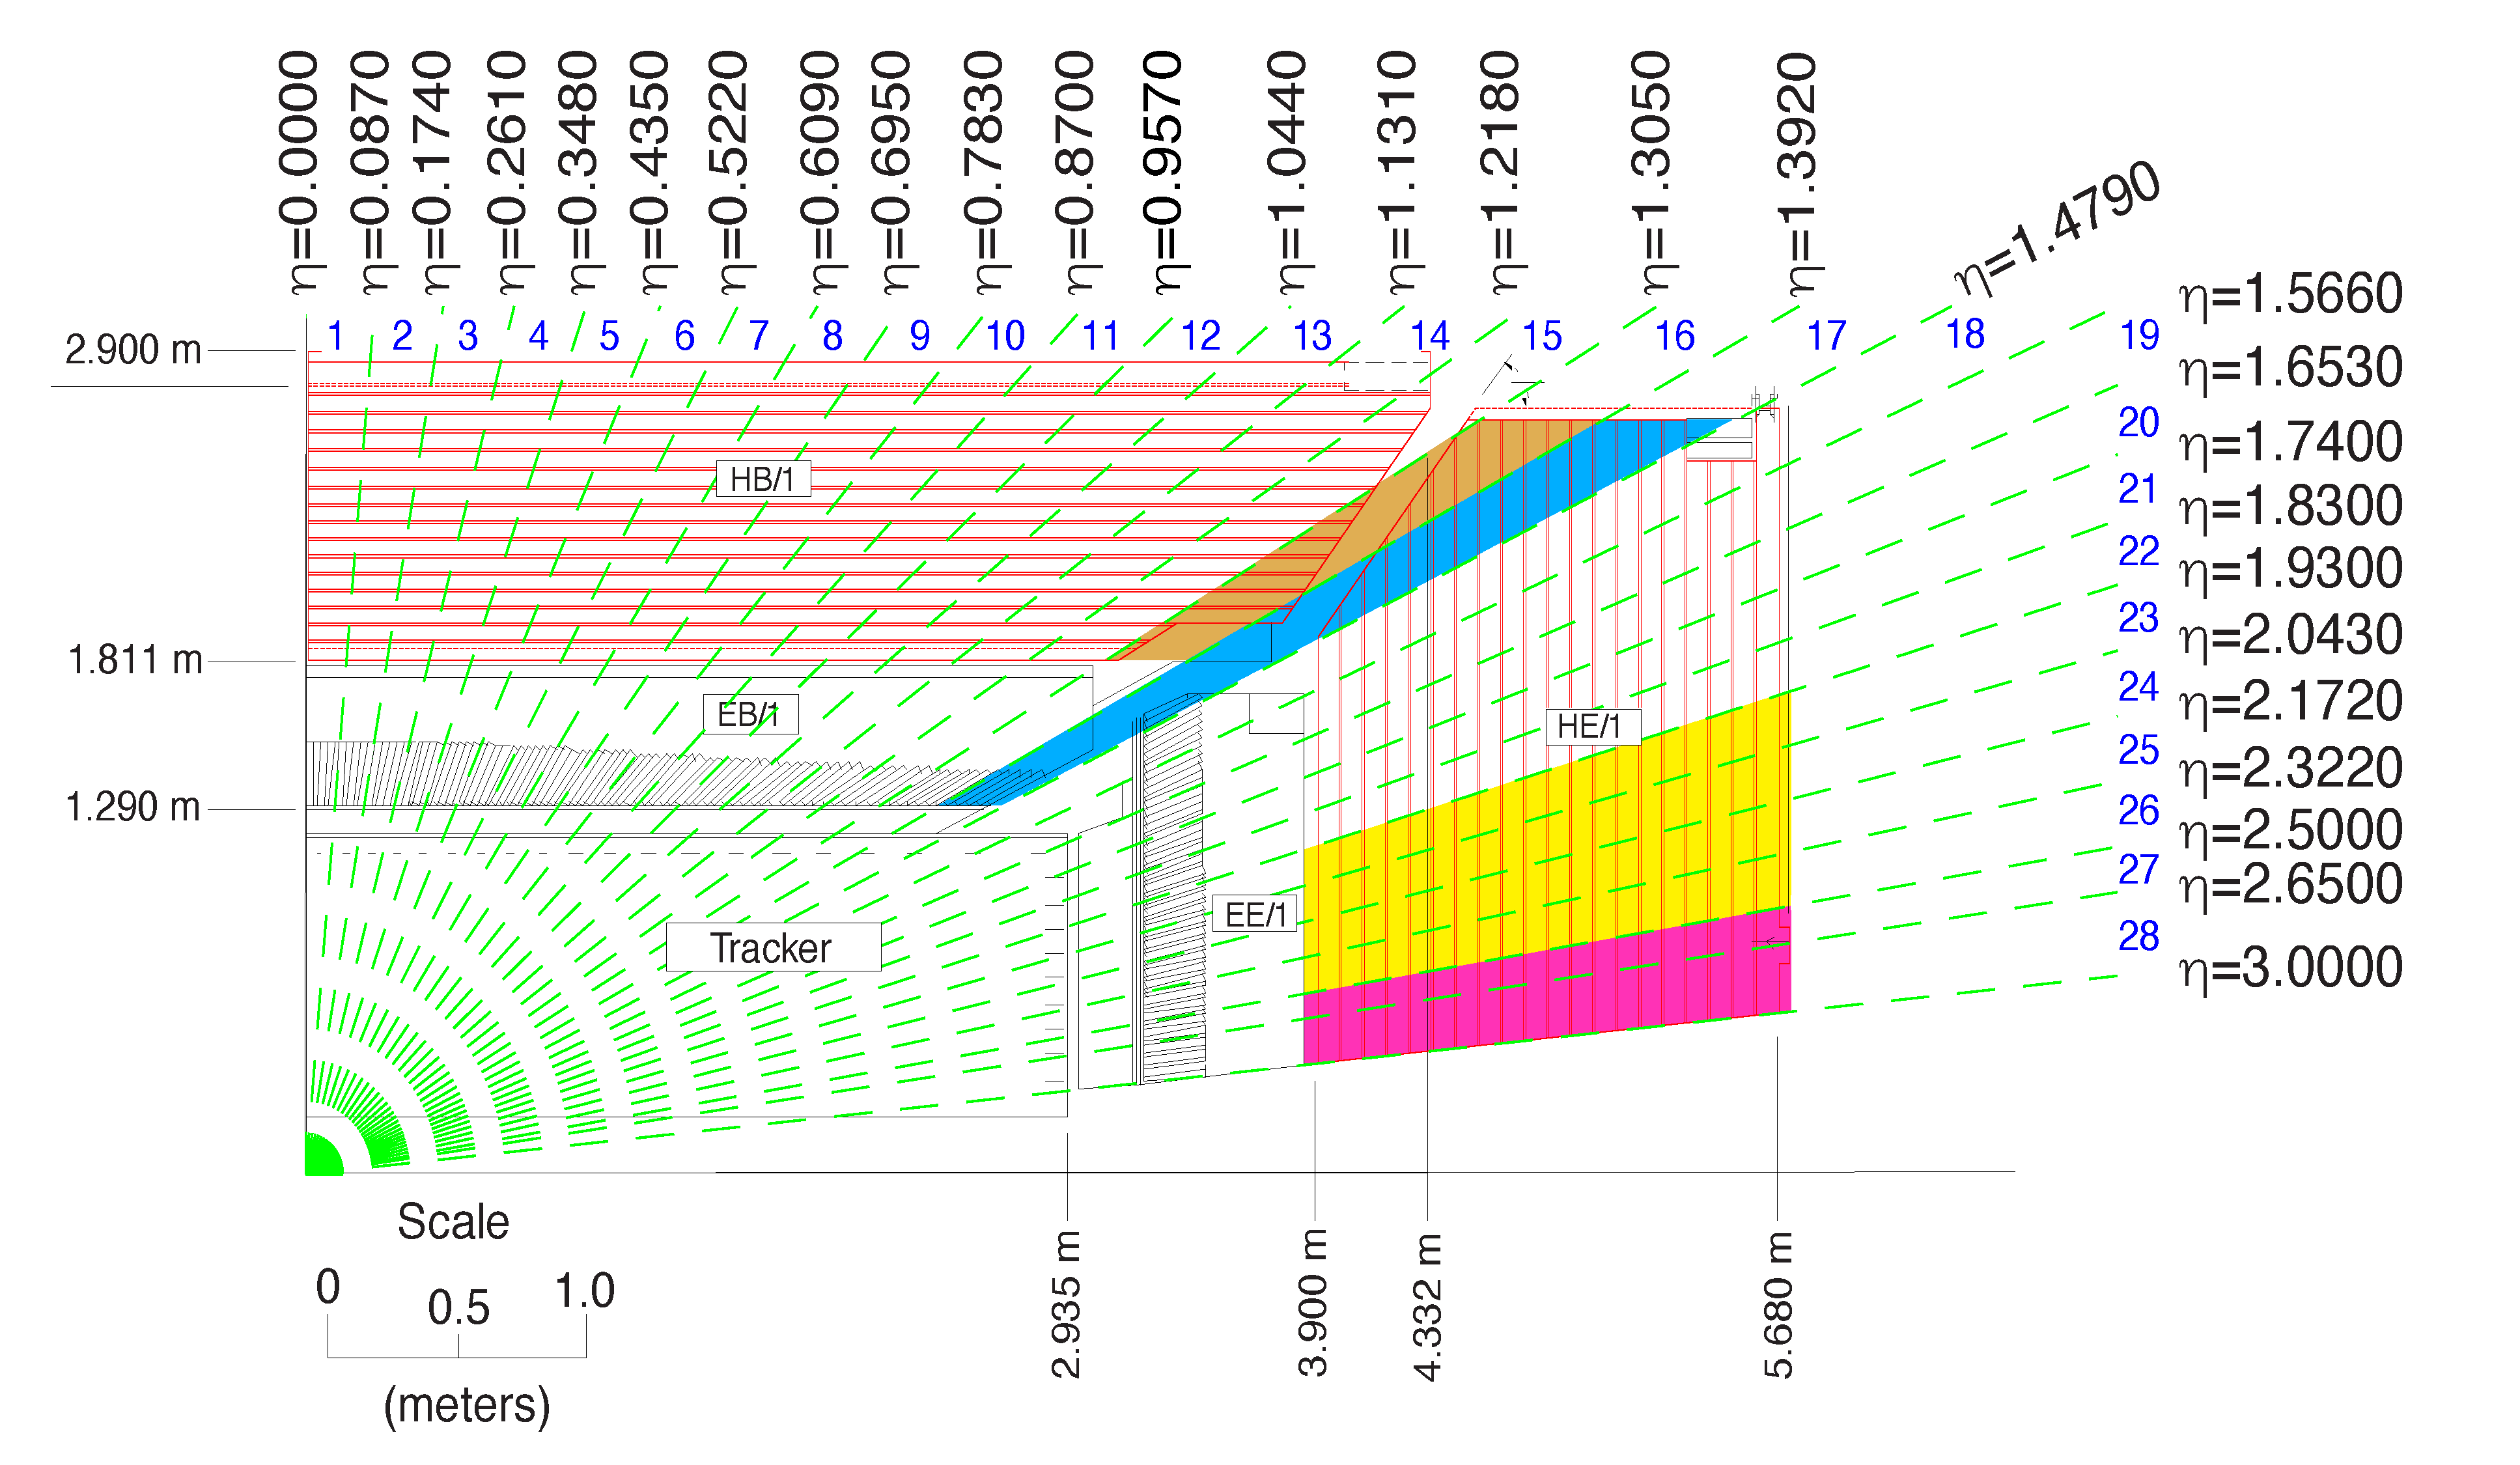
\includegraphics[width=0.9\linewidth]{Figures/L1TP/L1TP.pdf}
    \caption{Schematic view of the ECAL and HCAL TP separation in the $r$-$z$ projection of the CMS detector. }
    \label{fig:Layer1}
\end{figure}

\bigbreak

Each TP is characterised by a ($i\eta$, $i\phi$) position and a transverse energy, denoted as $E_T$.
The energy deposit is computed as the projection onto the transverse plane of the momentum vector originating in the detector centre and pointing to the calorimeter cells. This value is encoded into 8-bit digital quantities, corresponding to 256 possible values: each bit correspond to a 0.5~GeV unit, therefore each TP can transmit up to 127.5~GeV and higher values are saturated to the maximum.
The ($i\eta$, $i\phi$) position, instead, does not need to be encoded into digital quantities as it is fully determined by the linking in the detector read-out to the calorimeter trigger Layer-1.

The ECAL and HCAL TPs are transmitted to the Layer-1 calorimeter trigger, where a calibration factor is applied to each of them, based on position and energy deposit. Beside correcting for the detector non-homogeneity, the Layer-1 calibration can adjust the inter-calibration between the energy recorder in ECAL and HCAL TPs.
After the calibration, the ECAL and HCAL TPs that geometrically lie one behind the other are combined together into Trigger Towers (TTs).
A particular configuration is followed for the HF detector, where coarser TT granularity is adopted, with a segmentation of 4 TTs in $\eta$ and of 18 TTs in $\phi$ direction. 
Each TT is characterised by a 16-bit digital quantity that encodes a 9-bit word reporting the total $E_T$ from both ECAL and HCAL, the ratio of the ECAL and HCAL energies on 5 bits, and HCAL and ECAL quality flags on the 2 remaining bits.
At this stage, TTs can contain up to 255~GeV, and any TT with $E_T \geq 0.5$~GeV is referred to as an \textit{fired tower}. 
Finally, the Layer-1 sorts the TTs in descending $E_T$ order and transmits them to Layer-2, where any of the Master Processor (MP7) cards receives the complete set of TTs from each bunch crossing. 

\subsection{The Layer-2 calorimeter objects}
\label{subsec:The Layer-2 calorimeter objects}

In the Layer-2 calorimeter trigger, the TTs are merged together to form L1 objects. The L1 reconstruction algorithms have been developed and optimised to reconstruct electrons, photons, jets, hadronically decaying tau leptons, and energy sums.
Such algorithms need to access the full calorimeter information and require fast computing power furnished by Field-Programmable Gate Arrays (FPGAs) firmware.
A brief overview of the L1 calorimeter candidates reconstruction algorithms is given in the following paragraphs.

\subsubsection{Electrons and photon candidates}

Due to the unavailability of the tracking information at the L1 stage, electrons and photons are indistinguishable and grouped together in the $e/\gamma$ category, or \texttt{EGamma}.
The L1 $e/\gamma$ candidate is initiated by the presence of a high energy deposit in a single TT, also called \textit{seed}. The TTs around the seed are dynamically clustered~\cite{Sauvan_2015} to the seed according to their position and recorded energy.
The maximum cluster size is limited to 8 TTs, in order to minimise the impact of pile-up energy deposits while including most of the electron or photon energy.
Since electron and photon showers spread mostly along the $\phi$ direction due to the CMS magnetic field, an extended region in $\phi$ (5 TTs at most) and narrow in $\eta$ (2 TTs at most) is chosen.
The first and second neighbour fired TTs are clustered only if connected to the seed, as shown in Figure~\ref{fig:L1EGammaCluster}~(left).
The dynamic clustering leads to a large variety of cluster shapes depending on the distribution of the energy around the seed tower. Large clusters involving many trigger towers are probably produced by the pre-showering of jets in ECAL, while small clusters, containing typically one to four TTs, are more compatible with electron or photon showers. For this reason, the shape of the cluster, which would not be available for a fixed size clustering, is an important information for the particle candidate and brings additional discrimination power between electrons (or photons) and jets.

The sum of the ECAL $E_T$ of the seed and clustered towers is considered the raw $E_T$ of the $e/\gamma$ cluster, which is calibrated using Layer-2 scale factors dependent on the $\eta$-position of the seed tower. These calibration factors, derived from $Z \rightarrow ee$ events, are defined as the ratio of the offline reconstructed electron $E_T$ to the corresponding raw L1 cluster $E_T$.
Since the Layer-2 calorimeter trigger has access to TTs without boundaries, it is possible to account for the pile-up conditions by applying isolation requirements. The isolation energy is computed in a $5\time9$ TTs region, excluding the $e/\gamma$ candidate footprint in ECAL ($2\times5$ TTs) and HCAL ($1\times2$ TTs). The isolation region is better illustrated in Figure~\ref{fig:L1EGammaCluster}~(right). The isolation threshold depends on the $i\eta$ position of the cluster and on an estimator for the number of pile-up interactions, given by the number of TTs in the whole detector acceptance recording an energy $E_T>4$~GeV. 
Finally, an energy-dependent threshold on the ration between ECAL and HCAL energy deposit, also known as $E/H$, is applied to reduce the mis-identification rate of hadronic showers.

\begin{figure}
    \centering
    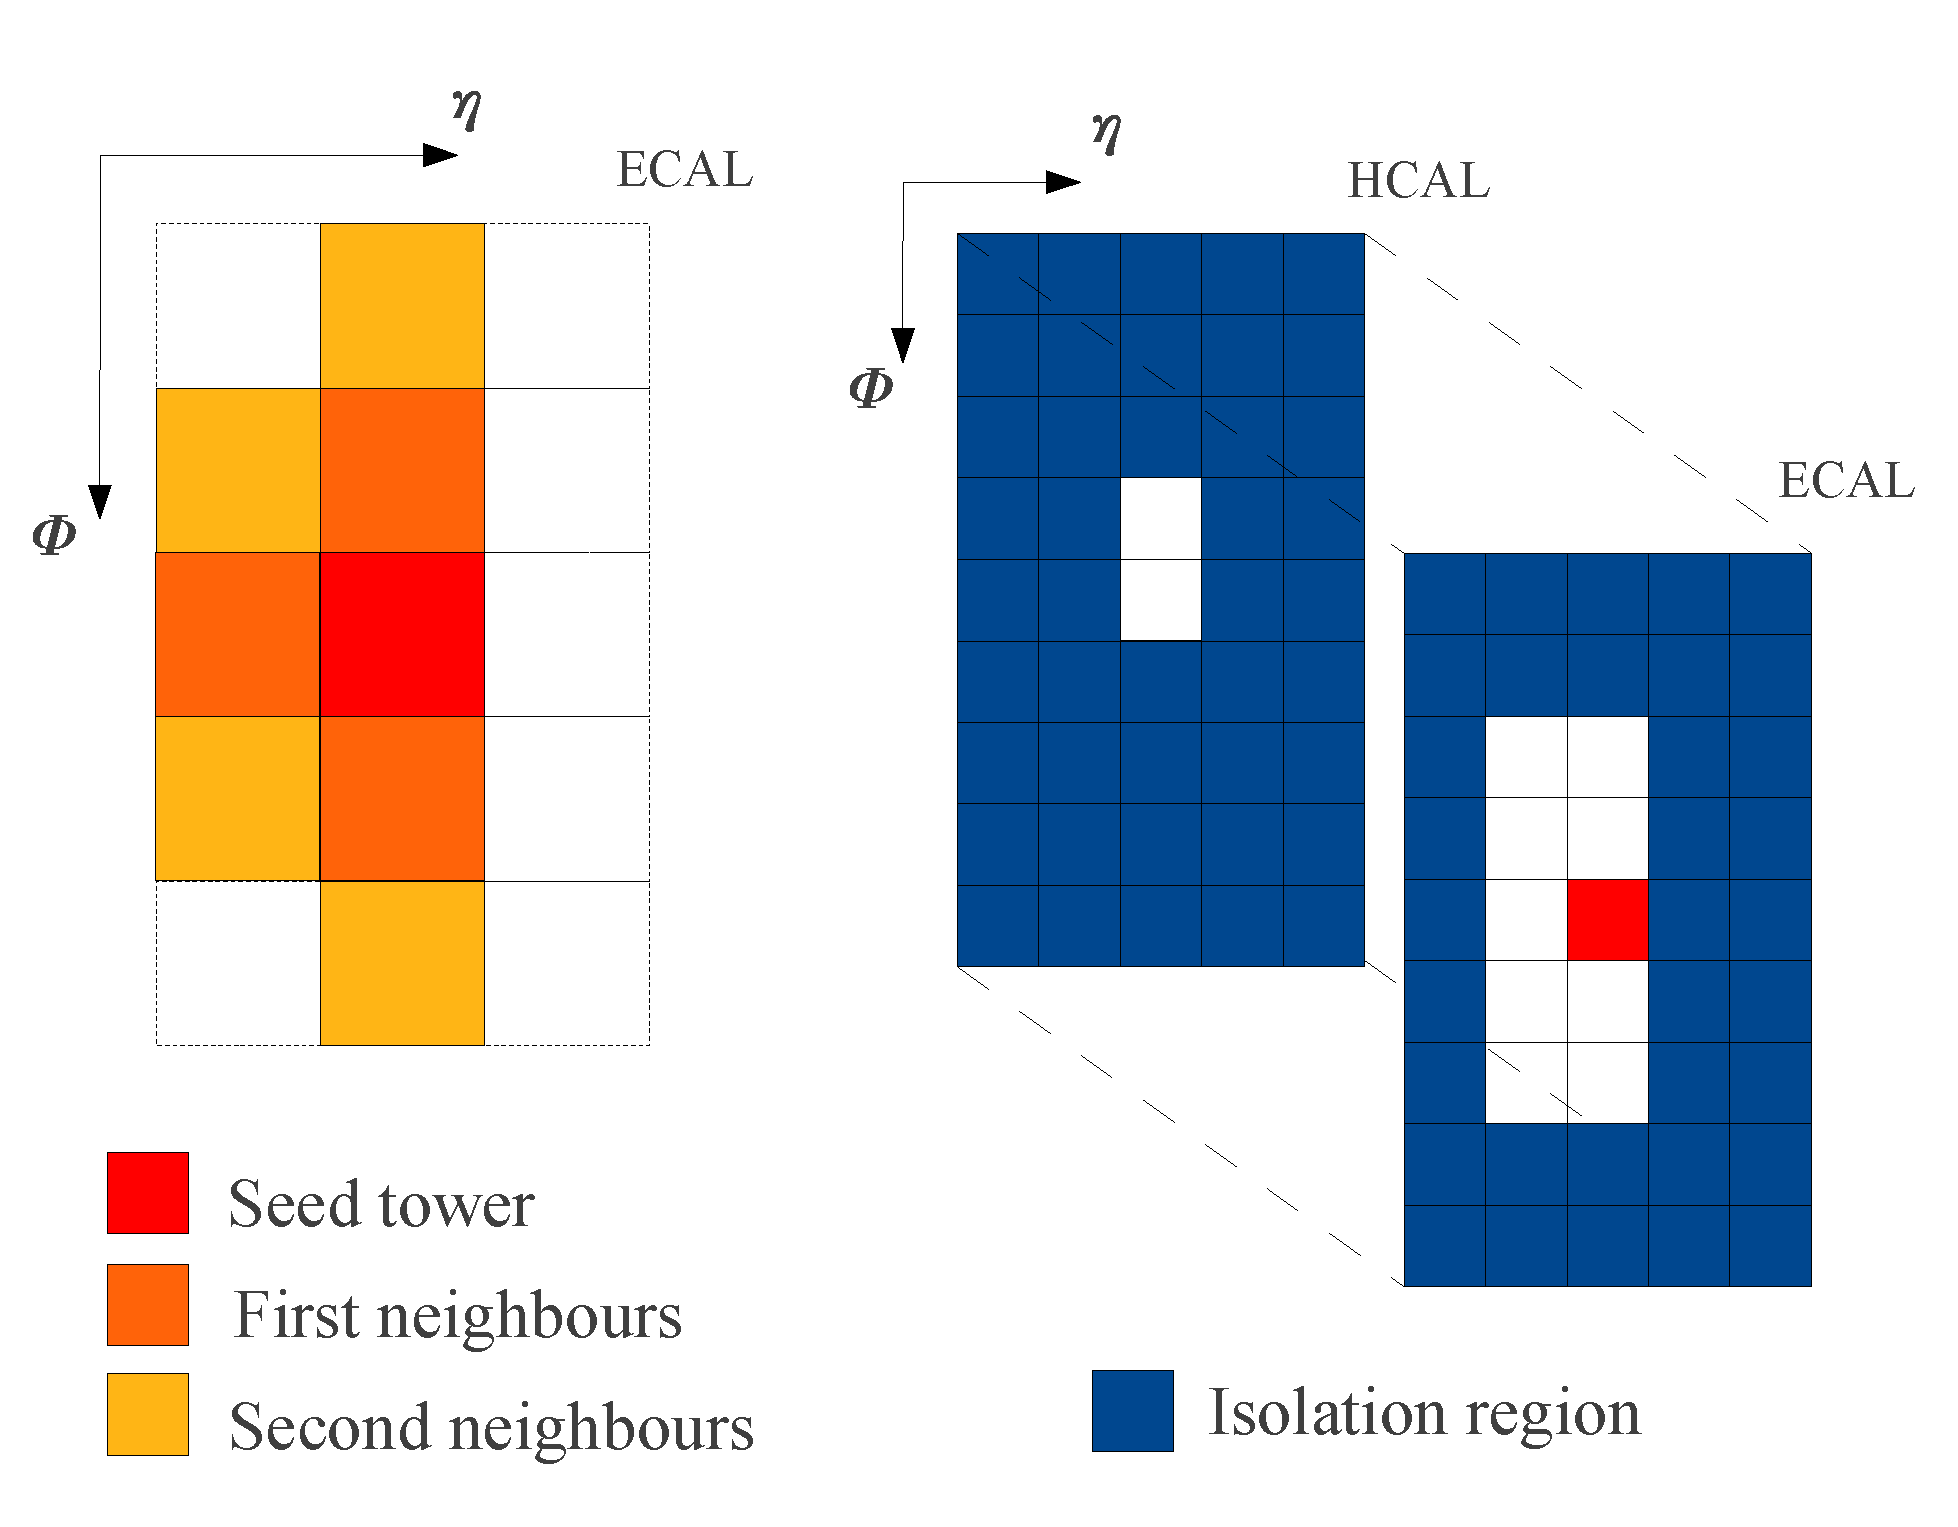
\includegraphics[width=0.5\linewidth]{Figures/L1TP/L1EGammaCluster.pdf}
    \caption{Schematic for the L1 $e/\gamma$ dynamic clustering and isolation. A candidate is formed by clustering around the seed all the fired neighbour towers. A candidate is considered as isolated if the $E_T$ in the ECAL and HCAL isolation regions is smaller than a given value.}
    \label{fig:L1EGammaCluster}
\end{figure}

\subsubsection{Hadronic tau lepton candidates}

Hadronically decaying $\tau$ leptons are reconstructed by the Layer-2 calorimeter trigger with an algorithm similar to the one used for $e/\gamma$ candidates.
The most probable products for the tau leptons hadronic decay are pions, which can leave energy deposit both in the ECAL and the HCAL calorimeters. 
The $\tau_h$ candidate selection begins a single TT seed, and the TTs around the seed, in a region spanning 5 and 9 TTs in the $\eta$ and $\phi$ directions respectively, are merged following the dynamic cluster procedure.
The TTs within one unit in $i\eta$ and $i\phi$ from the seed, and the ones on the same $i\eta$ position at two units distance in $i\phi$, are incorporated into the \textit{proto-cluster}. A subsequent \textit{lateral trimming} procedure is implemented to remove the least energetic side of the proto-cluster, as shown in Figure~\ref{fig:L1TauCluster}~(left).

Since the $\tau_h$ decay can produce several charged or neutral pions, leading to broader energy deposit. 
For this reason, at the same as the primary proto-cluster creation, \textit{secondary clusters} are built with the same approach, but considering a smaller window spanning 3 TTs in both $\eta$ and $\phi$ directions.
The secondary clusters are merged to the primary proto-cluster only if their seed is found in one of the eight positions highlighted in green in Figure~\ref{fig:L1TauCluster}~(right). An overlap procedure is applied to avoid double-counting of TTs in multiple clusters.
The sum of all the TTs $E_T$ included in the merged cluster is considered to be the raw $E_T$ of the $\tau_h$ cluster, which is calibrated using Layer-2 scale factors dependent on raw energy deposit, the $\eta$-position of the seed tower, the presence of ECAL energy deposit, and the cluster being issued by the merging procedure or not.
Also for $\tau_h$ candidates, an isolation requirement is applied to reduce contamination from hadronic jets, characterised by wider calorimeter activity. The isolation energy is computed in a $6\time9$ TTs region, excluding the $\tau_h$ candidate footprint.
The isolation threshold depends on the raw energy deposit, on the $i\eta$ position of the cluster, and on an estimator for the number of pile-up interactions, given by the number of fired TTs in the most central region of the barrel, i.e. $|i\eta|\leq 4$.

\begin{figure}
    \centering
    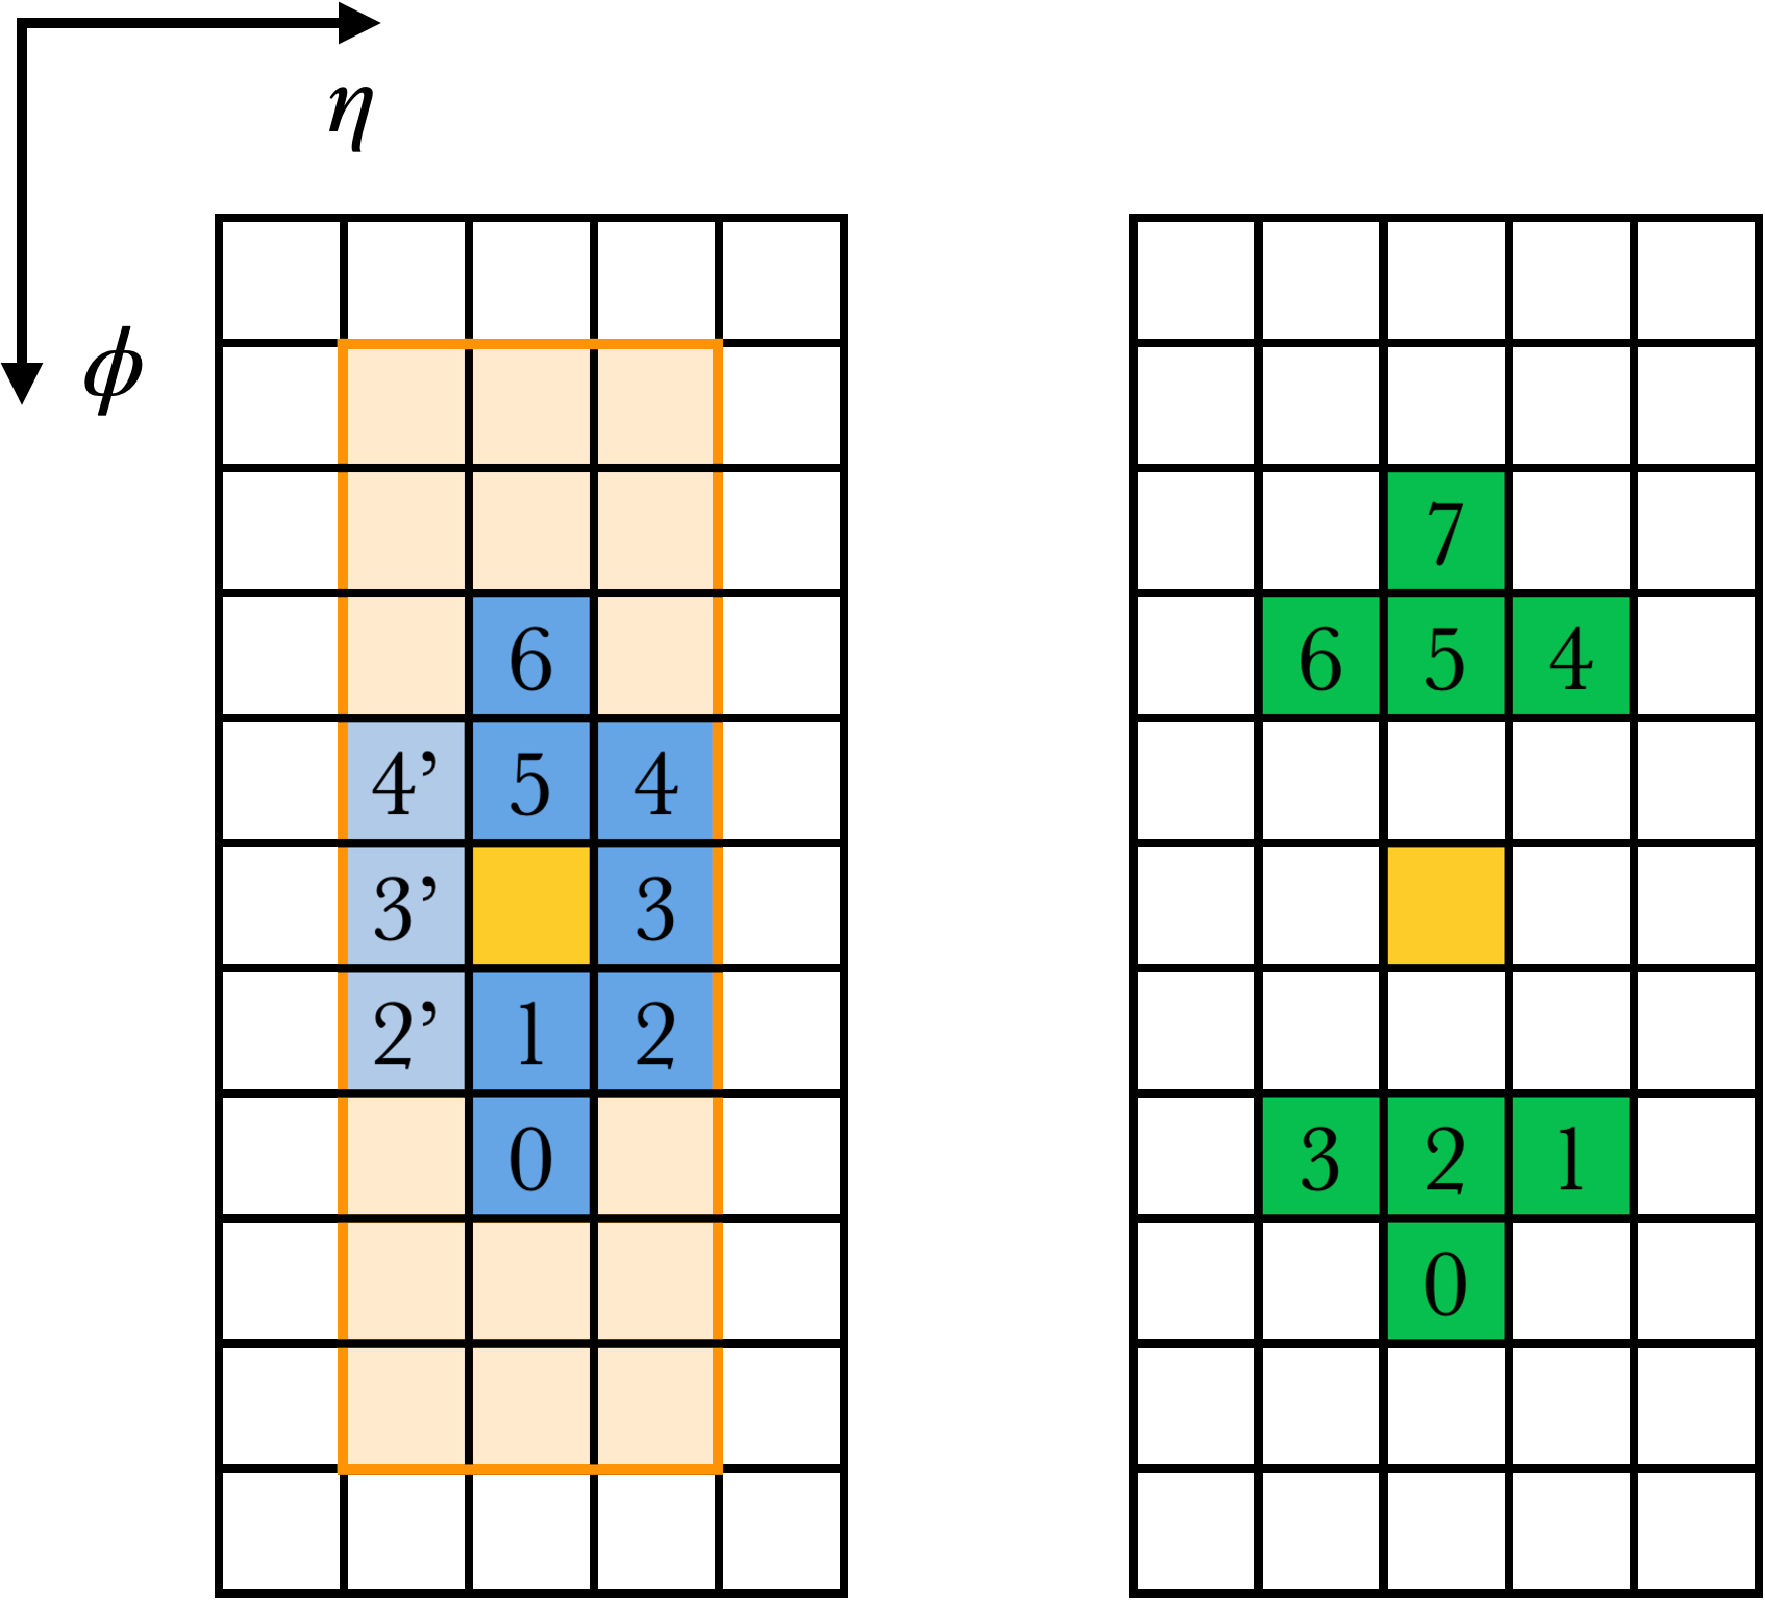
\includegraphics[width=0.4\linewidth]{Figures/L1TP/L1TauCluster.pdf}
    \caption{Schematic for the $\tau_h$ dynamic clustering algorithm. A candidate is initiated by the definition of a proto-clustering, consequently trimmed to remove the least energetic side (left). Additional secondary clusters can be merged to the primary one, if their seed lies within the seven green TTs (right); the secondary clusters seeded in position 2 or 5 are not considered if their seed is already included in the primary proto-cluster.}
    \label{fig:L1TauCluster}
\end{figure}

\subsubsection{Jet candidates}

The hadronic jet candidates are defined from a fixed dimension clustering approach. 
The L1 jet candidate is initiated by the presence of a high energy deposit in a single TT seed, and the surrounding matrix of $9\times9$ TTs defines as the jet cluster. 
The size of the window is chosen to correspond to the $\Delta R = 0.4$ angular opening, which is radius used for the offline anti-$k_T$ reconstruction algorithm~\cite{Zabi_2016}.
In order to avoid double counting of jets, a jet candidate is discarded if any of the TTs composing the cluster has an energy deposit greater than the central seed.
The energy in the $9\times9$ cluster, also known as \textit{chunky donut}, is defined to be the raw jet energy.

Given the large extension of the jet candidate, a dedicate pile-up subtraction method is implemented, which estimates the energy deposit due to pile-up and subtracts it to the jet raw energy deposit.
Two techniques for local pile-up correction are available in the Layer-2 algorithm employed during Run~III data taking:
\begin{itemize}
    \item Chunky donut subtraction: the pile-up energy is estimated as the sum of the energy deposit in the four $9\times3$ strips around the chunky donut, removing the highest and lowest energy sides.
    \item Phi-ring subtraction: the pile-up energy is estimated as the energy deposit on 9 rings of TTs with the same $\eta$ coordinates, re-scaling the surface to the $9\times9$ of the jet candidate.
\end{itemize}

As a last step, the Layer-2 jet candidates are calibrated based on their raw energy and $\eta$ position.

\begin{figure}
    \centering
    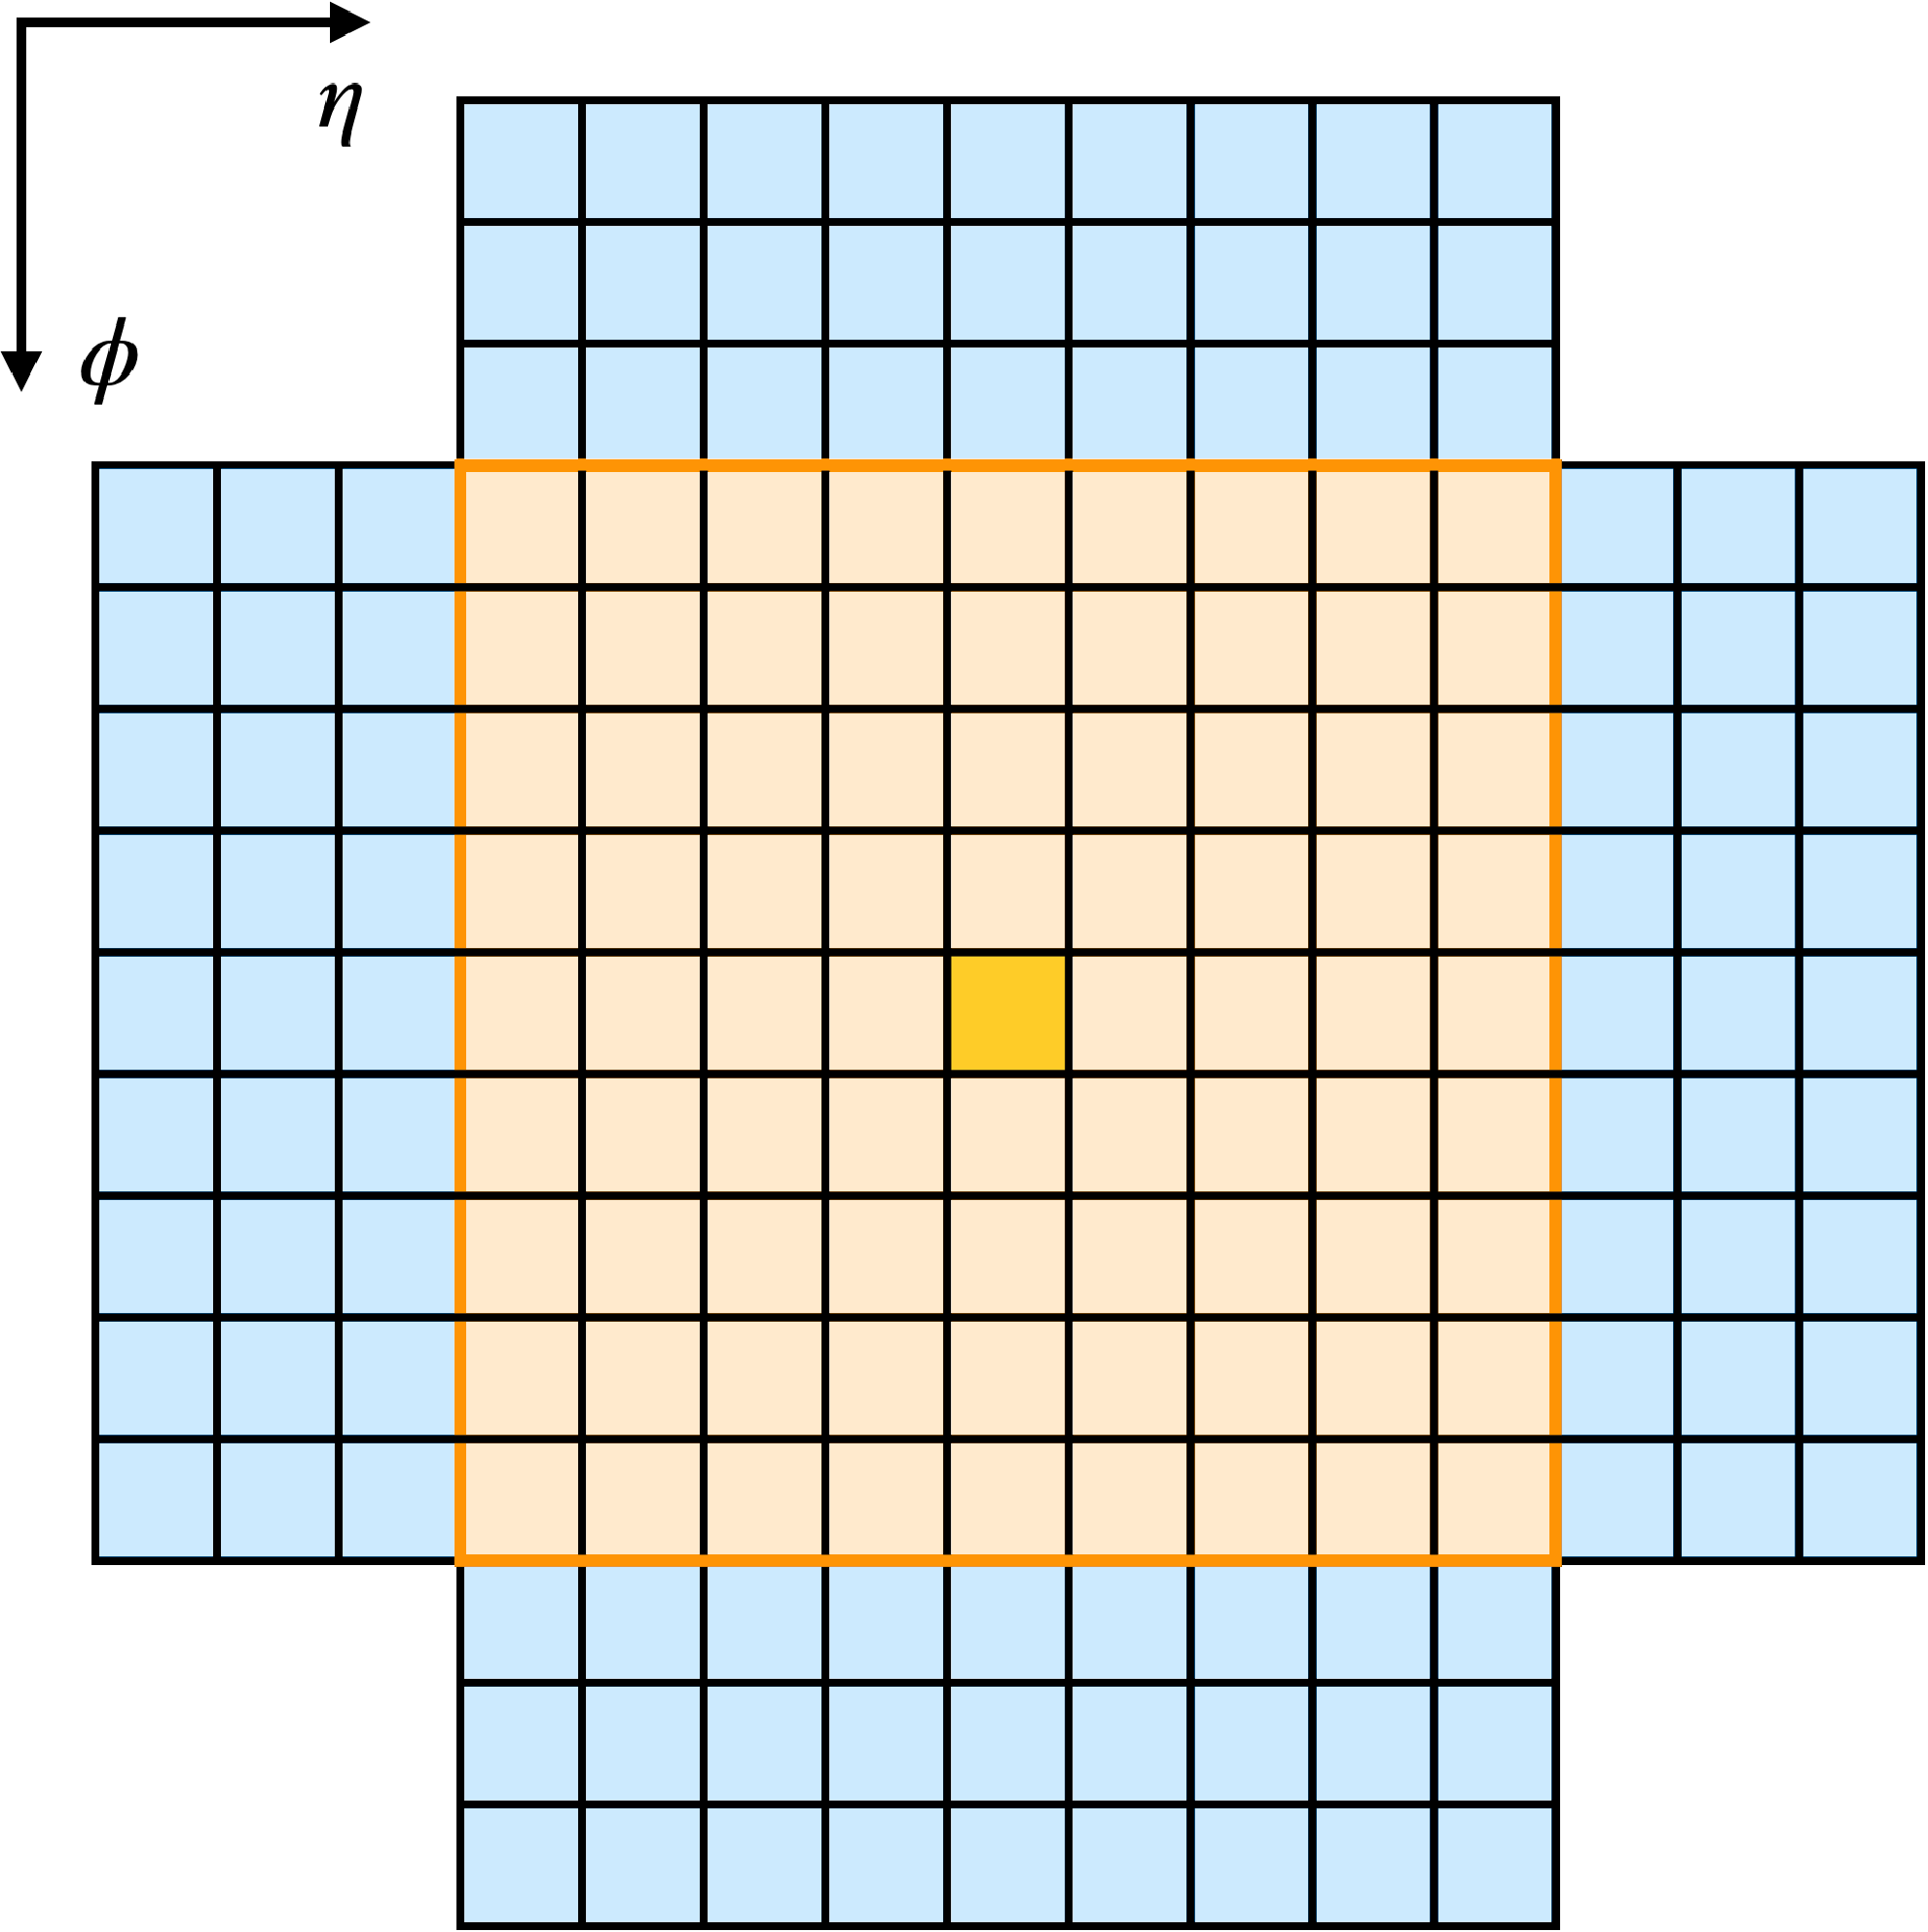
\includegraphics[width=0.4\linewidth]{Figures/L1TP/L1JetCluster.pdf}
    \caption{Schematic for the jet $9\times9$ chunky donut cluster. The four calorimeter strips around the chunky donut are used to estimate the local energy density due to piel-up.}
    \label{fig:L1JetCluster}
\end{figure}

\subsubsection{Energy sums candidates}

The energy sums are the last objects to be constructed in the L1 calorimeter trigger, as they involve full calorimeter granularity.
The total missing transverse energy $E_T^{miss}$ is computed by splitting the regional TTs energies into their $x$ and $y$ components, and summing the components in quadrature.
The resulting vector, after a rotation of $180^{\circ}$, provides the magnituse and angle of the missing energy due to neutrinos not interacting with the detector material.
The total scalar transverse energy of all jets $H_T$ is given by the sum over all clustered jets found in the event.
A dedicated pile-up subtraction and calibration is applied to $E_T^{miss}$ candidate to remove the large contribution coming from soft, diffuse pile-up energy deposits.
The pile-up contribution is estimated from the tower activity in the central part of the barrel and 

\begin{figure}
    \centering
    \subfloat[]{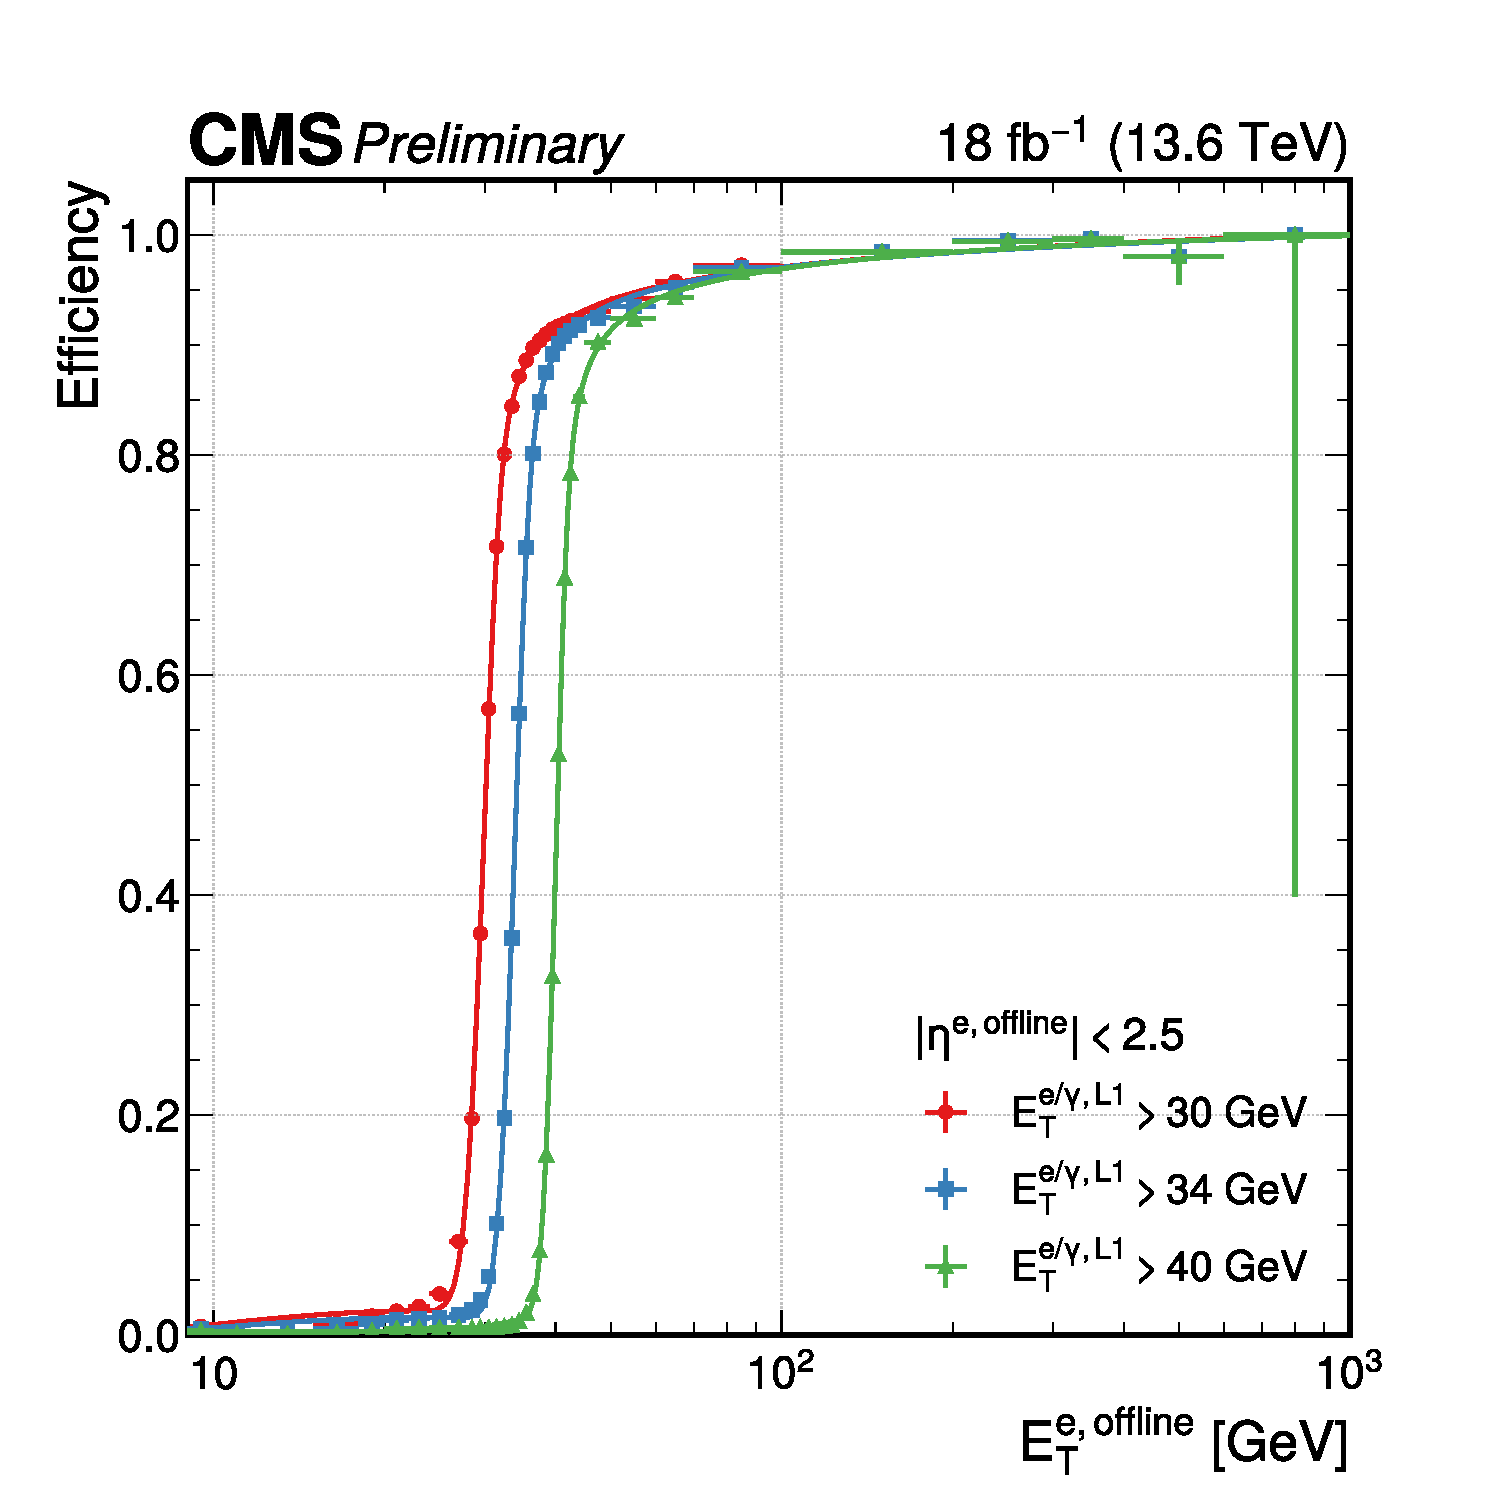
\includegraphics[width=0.4\linewidth]{Figures/L1TP/EGEfficiency.pdf}}
    \subfloat[]{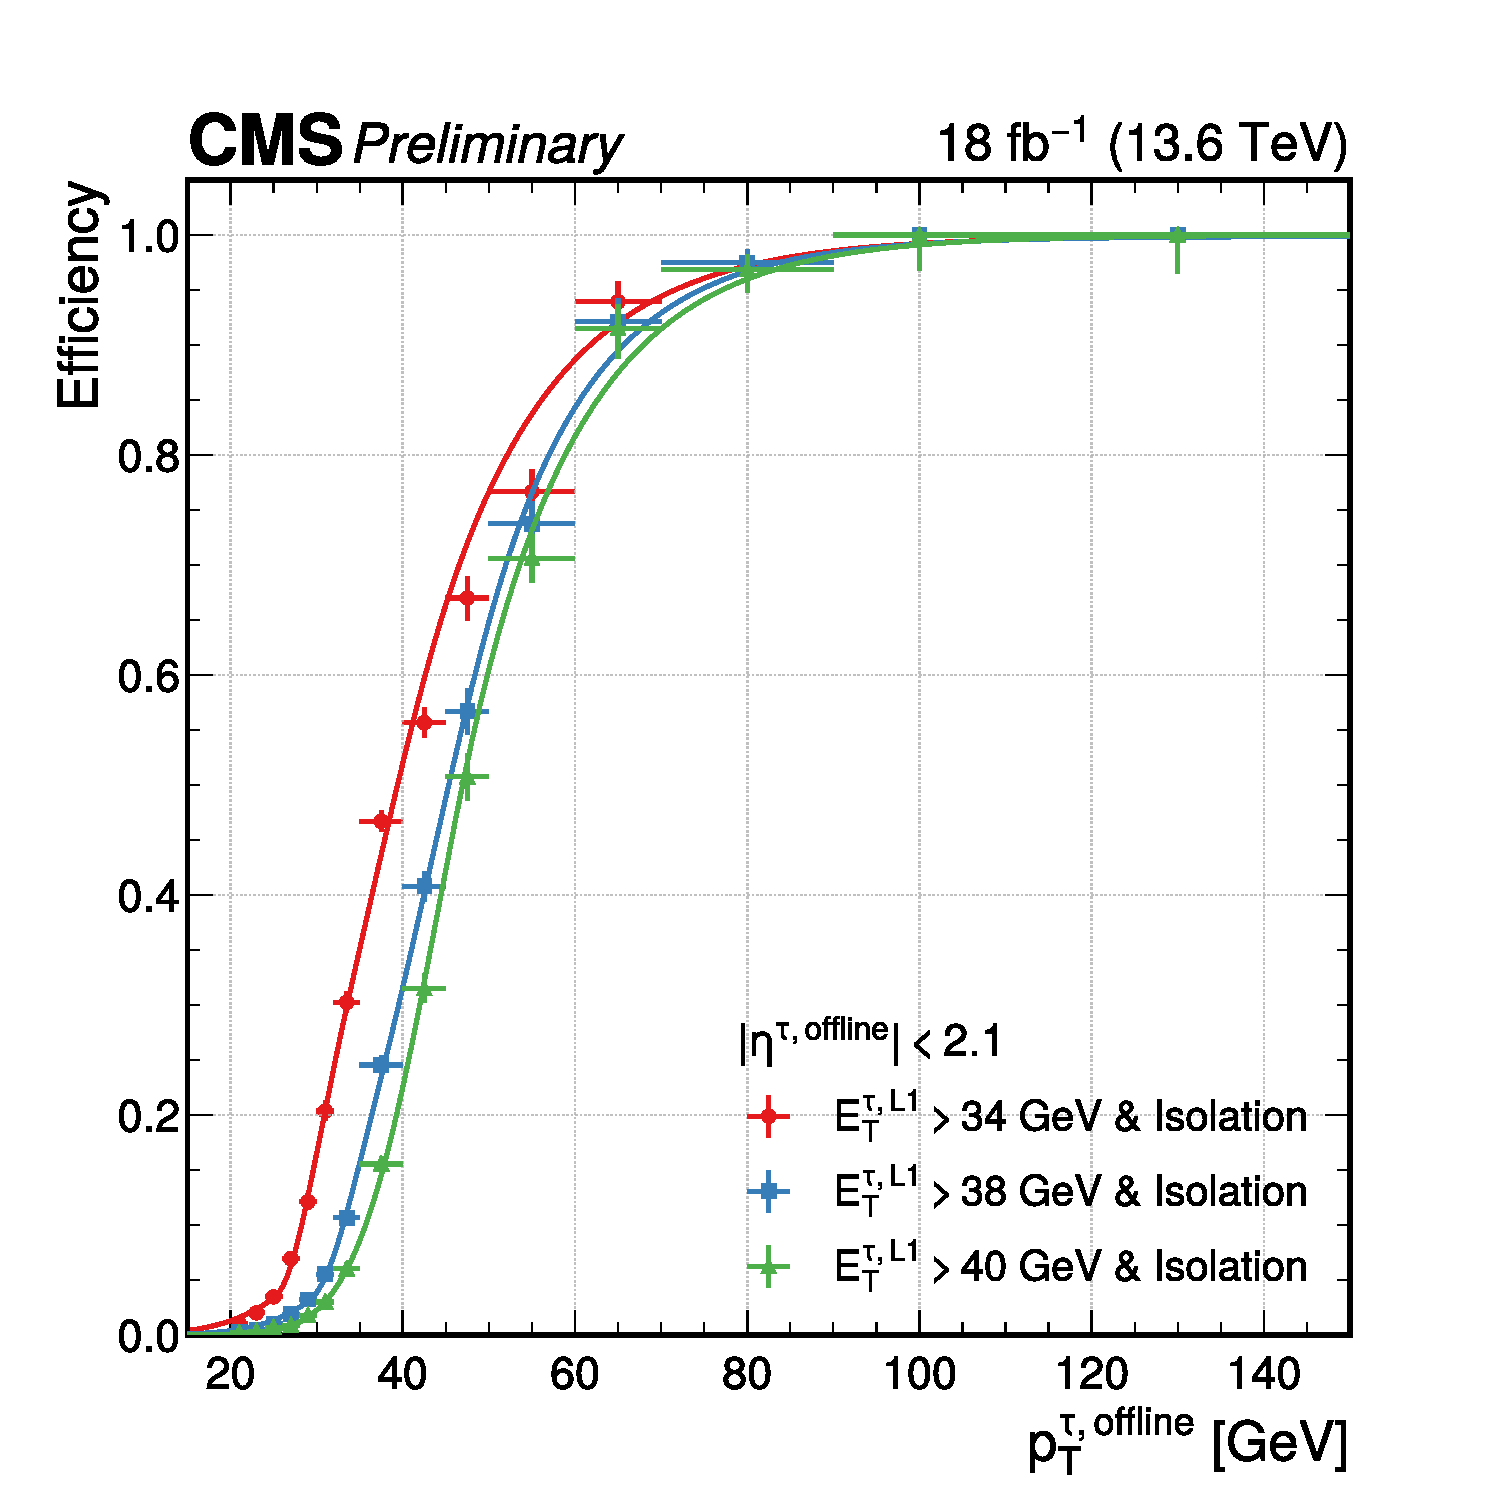
\includegraphics[width=0.4\linewidth]{Figures/L1TP/TauEfficiency.pdf}}
    
    \subfloat[]{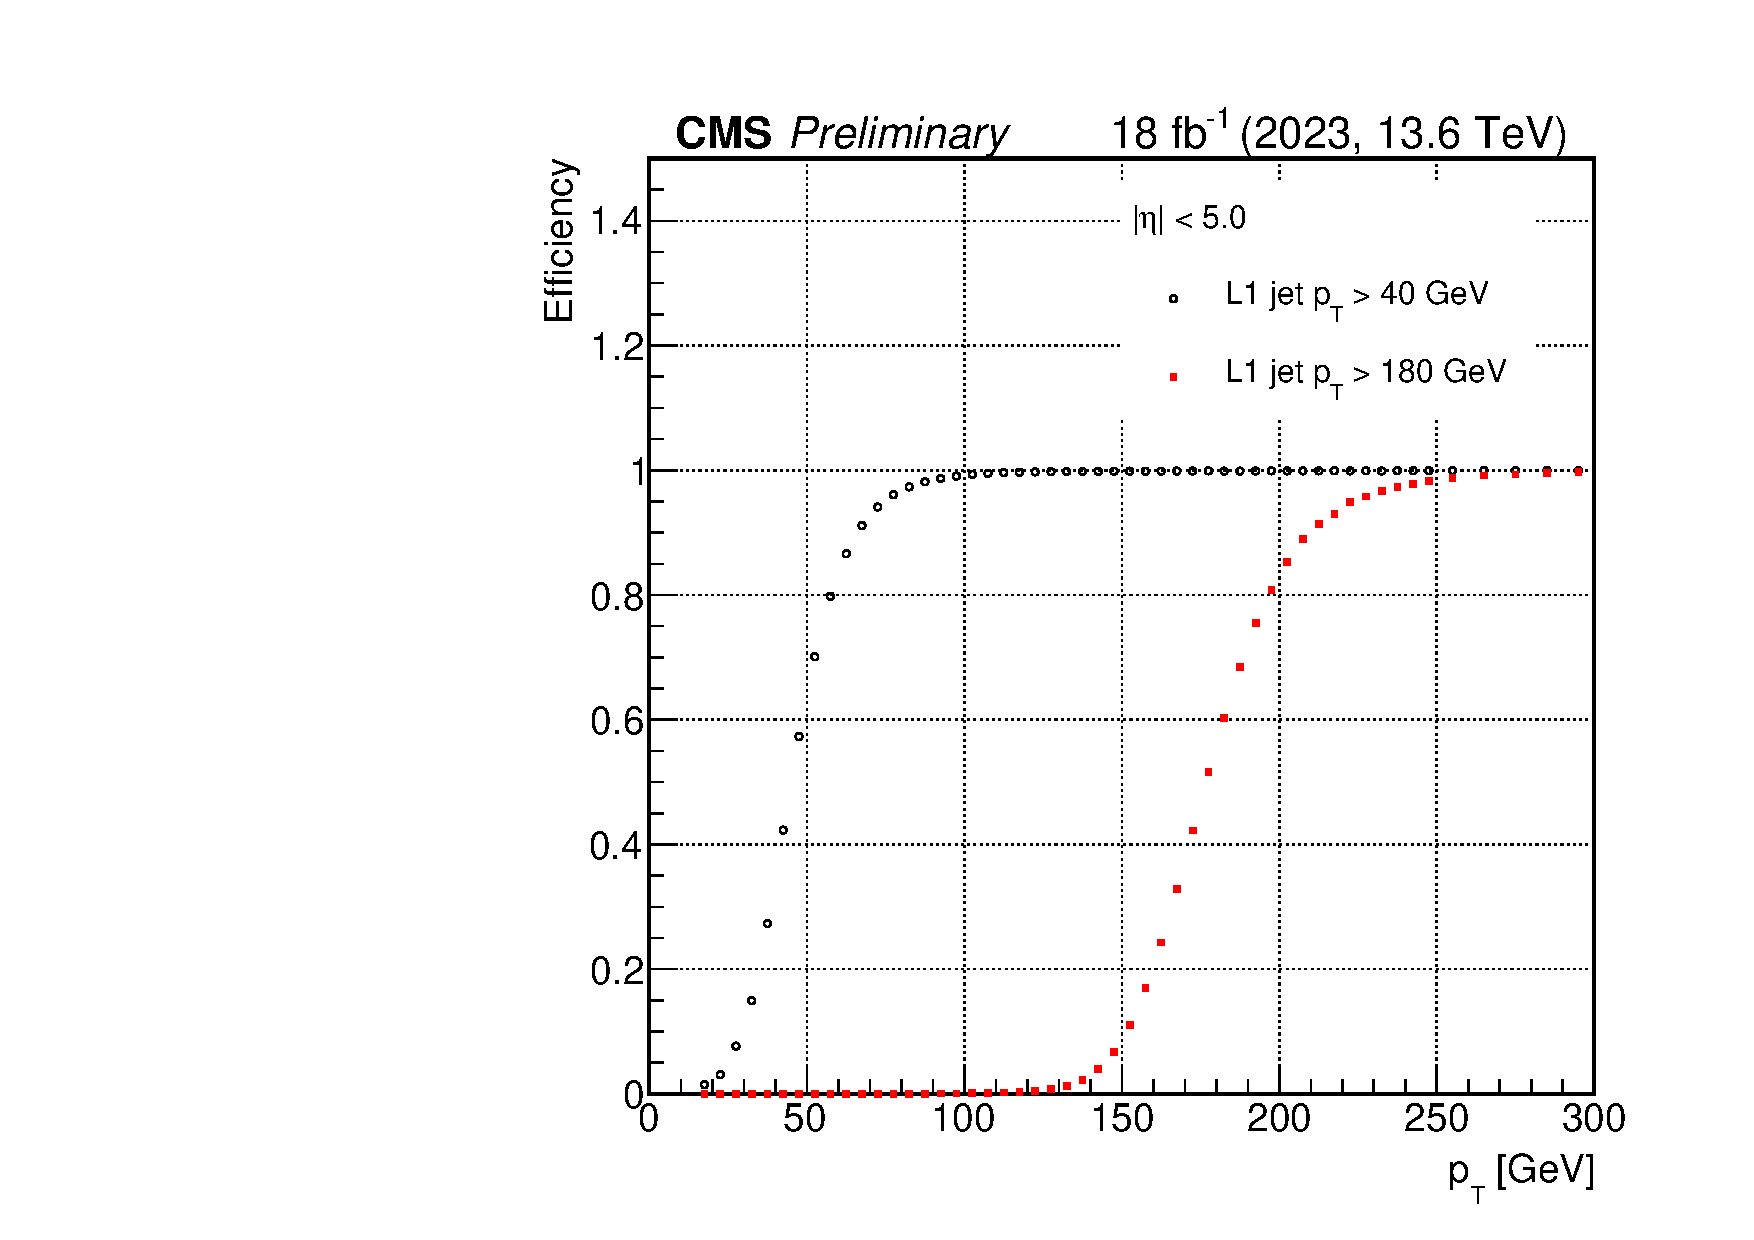
\includegraphics[width=0.4\linewidth]{Figures/L1TP/JetEfficiency.pdf}}
    \subfloat[]{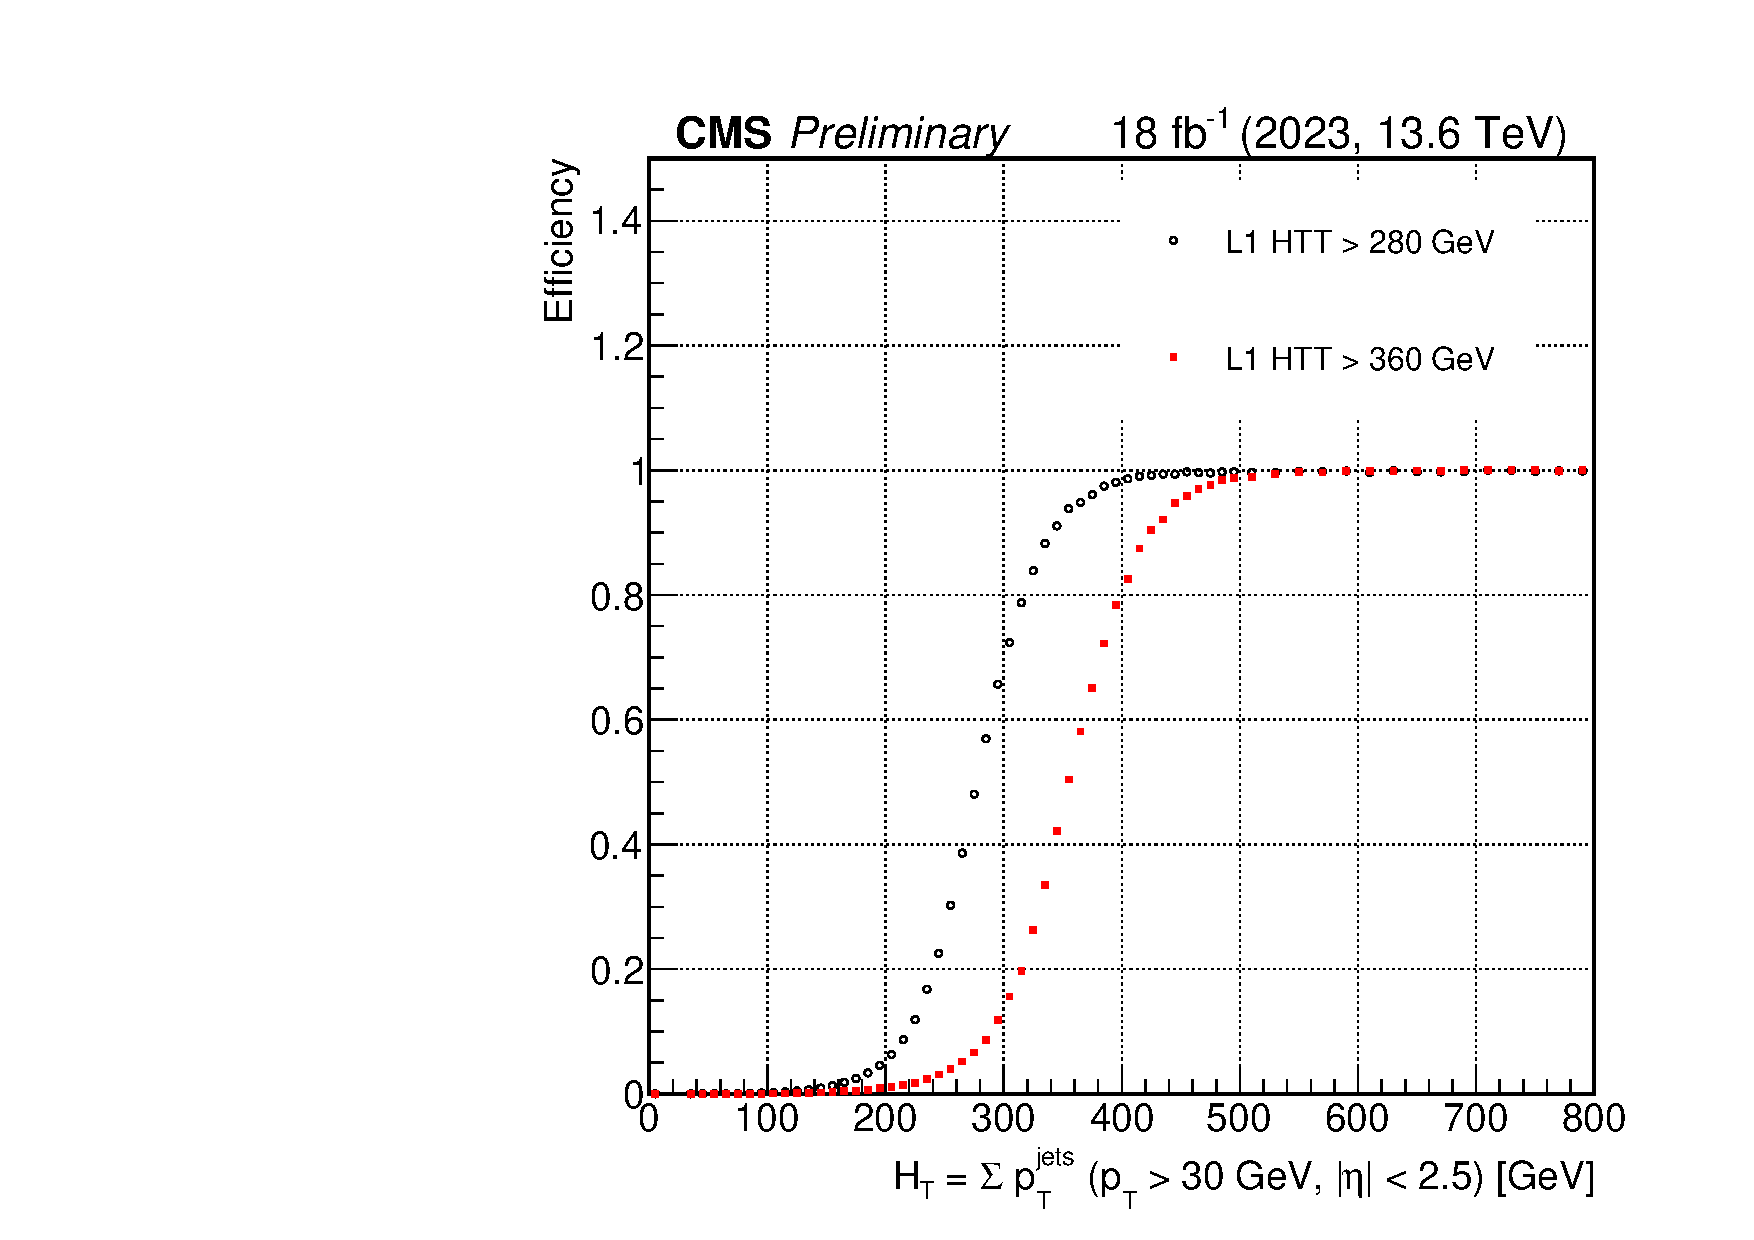
\includegraphics[width=0.4\linewidth]{Figures/L1TP/HTTEfficiency.pdf}}
    \caption{Level-1 performance of L1 calorimeter trigger objects: $e/\gamma$ (a), $\tau_h$ (b), jet (c), and $H_T$ (d). The efficiency turn-on curves are reported for different L1 $p_T$ thresholds.}
    \label{fig:L1Efficiency}
\end{figure}

\bigbreak

The performance of the L1 calorimeter trigger in finding the objects candidate and computing their energy is summarised in Figure~\ref{fig:L1Efficiency}, in terms of efficiency turn-on curves.
The reader will understand, at this point, the considerable importance of Layer-1 calibration in building the L1 calorimeter trigger candidates. 
Given the stacked architecture of Layer-1 and Layer-2, where the latter is fully dependent of the former's output, a better calibration of the TPs at Layer-1 can be crucial in improving the Layer-2 performance.

\section{The current Layer-1 calibration method}
\label{sec:The current Layer-1 calibration}

A first method to extract Layer-1 calibration factors was developed at the beginning of Run~II. 
The approach relies on the extraction of firmware-compatible calibration factors to be applied to the ECAL and HCAL TPs arriving in the Layer-1 calorimeter trigger from the ECAL and HCAL read-out electronics.
The Layer-1 firmware supports a single calibration constant to be applied to each TP, depending on its $i\eta$ position and recorded raw energy.
In this method, the calibration factors are derived in exclusive regions of energy deposit and $i\eta$ position, by comparing the Layer-1 TT response from MC samples to the energy of generated objects~\cite{Sirunyan_2020}.

The ECAL TPs calibration factors are based on MC simulated events of single photon production in the ideal environment of no pile-up, with a flatten transverse momentum spectrum for the photon $p_T \in [0,200]$~GeV, and flatten $\eta$ distribution.
For each event, the generated photons are matched to the corresponding TP, based on the ($\eta$, $\phi$) position, which will be considered as the seed. The $e/\gamma$ candidate is approximated as the $3\times3$ cluster centered around the seed. 
Only clusters containing at least 90\% of the total energy in the central tower are considered for the calibration procedure.
The energy binning is defined according to the energy of the central TP, with a pre-defined binning $E_T\in[0,3,6,9,12,15,20,25,30,35,40,45,55,70,127.5]$~GeV.
The clusters are further divided into 28 bins according to the absolute $i\eta$ position of the central TP, i.e. $|i\eta|\leq28$.
In each ($E_T$, $i\eta$) bin, the differential distribution of the uncalibrated Layer-1 response, defined as the ratio between the generated photon transverse momentum and the $3\time3$ cluster energy deposit $p_T^{\gamma}/E_T^{3\times3}$, is interpolated with a Landau distribution convoluted with a Gaussian distribution.

The HCAL TPs calibration factors are obtained following the same procedure detailed above the ECAL, using a MC sample of double charged pion production in the ideal environment of no pile-up; the pions are characterised by a flatten transverse momentum spectrum $p_T\in[0,200]$~GeV and flatten $\eta$ distribution.
Since objects tend to deposit energy in ECAL before reaching HCAL, the HCAL calibration factors are derived considering ECAL TPs in their derivation, and applying the previously extracted ECAL Layer-1 calibration.
For each event, the generated pions are matched to the corresponding TP, based on the ($\eta$, $\phi$) position, and a window of $5\times5$ in ECAL and HCAL centered around the seeding TP is considered as the jet cluster candidate.
It should be noted that in this method the jet cluster size is significantly reduced with respect to the $9\times9$ chunky donut actually used in the Layer-2 algorithm.
Only clusters containing at least 20\% of the total energy in the central tower are considered for the calibration procedure.
The events are binned according to the energy of the central TP, with the same pre-defined binning as ECAL, and to its absolute $i\eta$ position, i.e. $|i\eta|\leq41 \setminus \{29\}$.
For the HF calibration factors, the ECAL contribution is not considered, as the ECAL detector is not present in that pseudorapidity region.
In both cases, saturated towers with energy $E_T=127.5$~GeV are ignored by the calibration procedure. 

The calibration factors are originally designed to be extracted by the mean of the fitted distribution; however, given the presence of large tails towards higher energies, the method has been upgraded in 2018 to use the mode, i.e. the value that appears most frequently in the distribution.
An example for the interpolation of the response distributions is reported in Figure~\ref{fig:OldL1Fit}, for ECAL $E_T \in [0,3]$~GeV and $i\eta=1$~(a), and for HF $E_T \in [0,3]$~GeV and $i\eta=31$~(b).

The extracted calibration constants are stored in three firmware-compatible Look-Up-Tables (LUT), for ECAL, HCAL, and HF respectively. In total, for 13 energy bins and 40 pseudorapidity rings, 520 scale factors are defined, and encoded into 10-bit digital variables.
The resulting values are summarised in Figure~\ref{fig:L1OldSF} for ECAL and HCAL TPs, as a function of $i\eta$ and $E_T$.
The increase of the calibration factors with $\eta$ reflects the profile of the detector material in front of the calorimeters. The choice of the binning respects the hardware limitation and takes into account the dependency of the resolution in $E_T$.

\begin{figure}
    \centering
    \subfloat[]{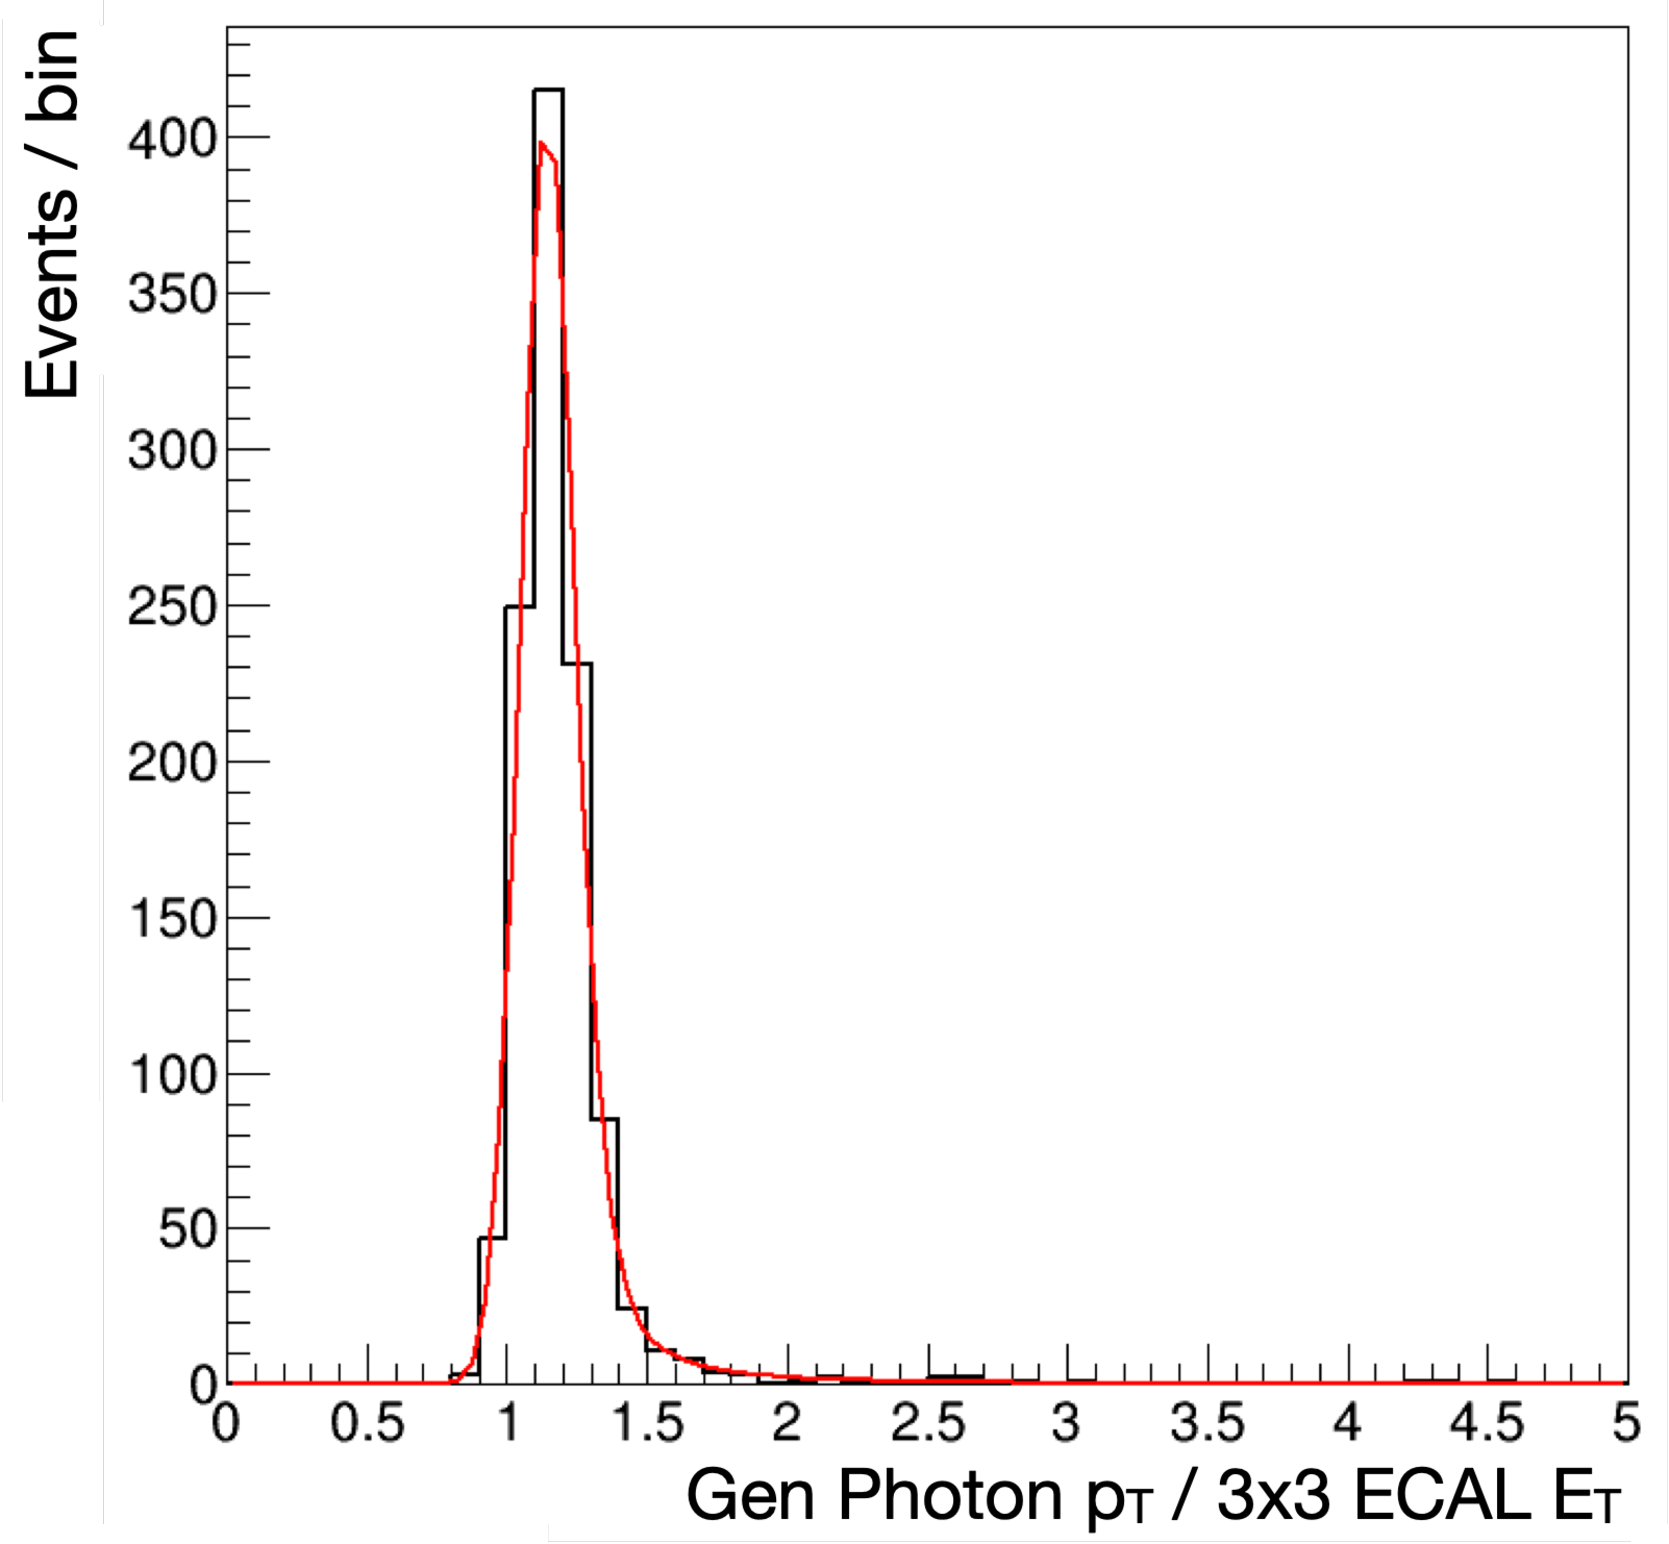
\includegraphics[width=0.4\linewidth]{Figures/L1TP/OldL1ECAL.pdf}}
    \hspace{0.7cm}
    \subfloat[]{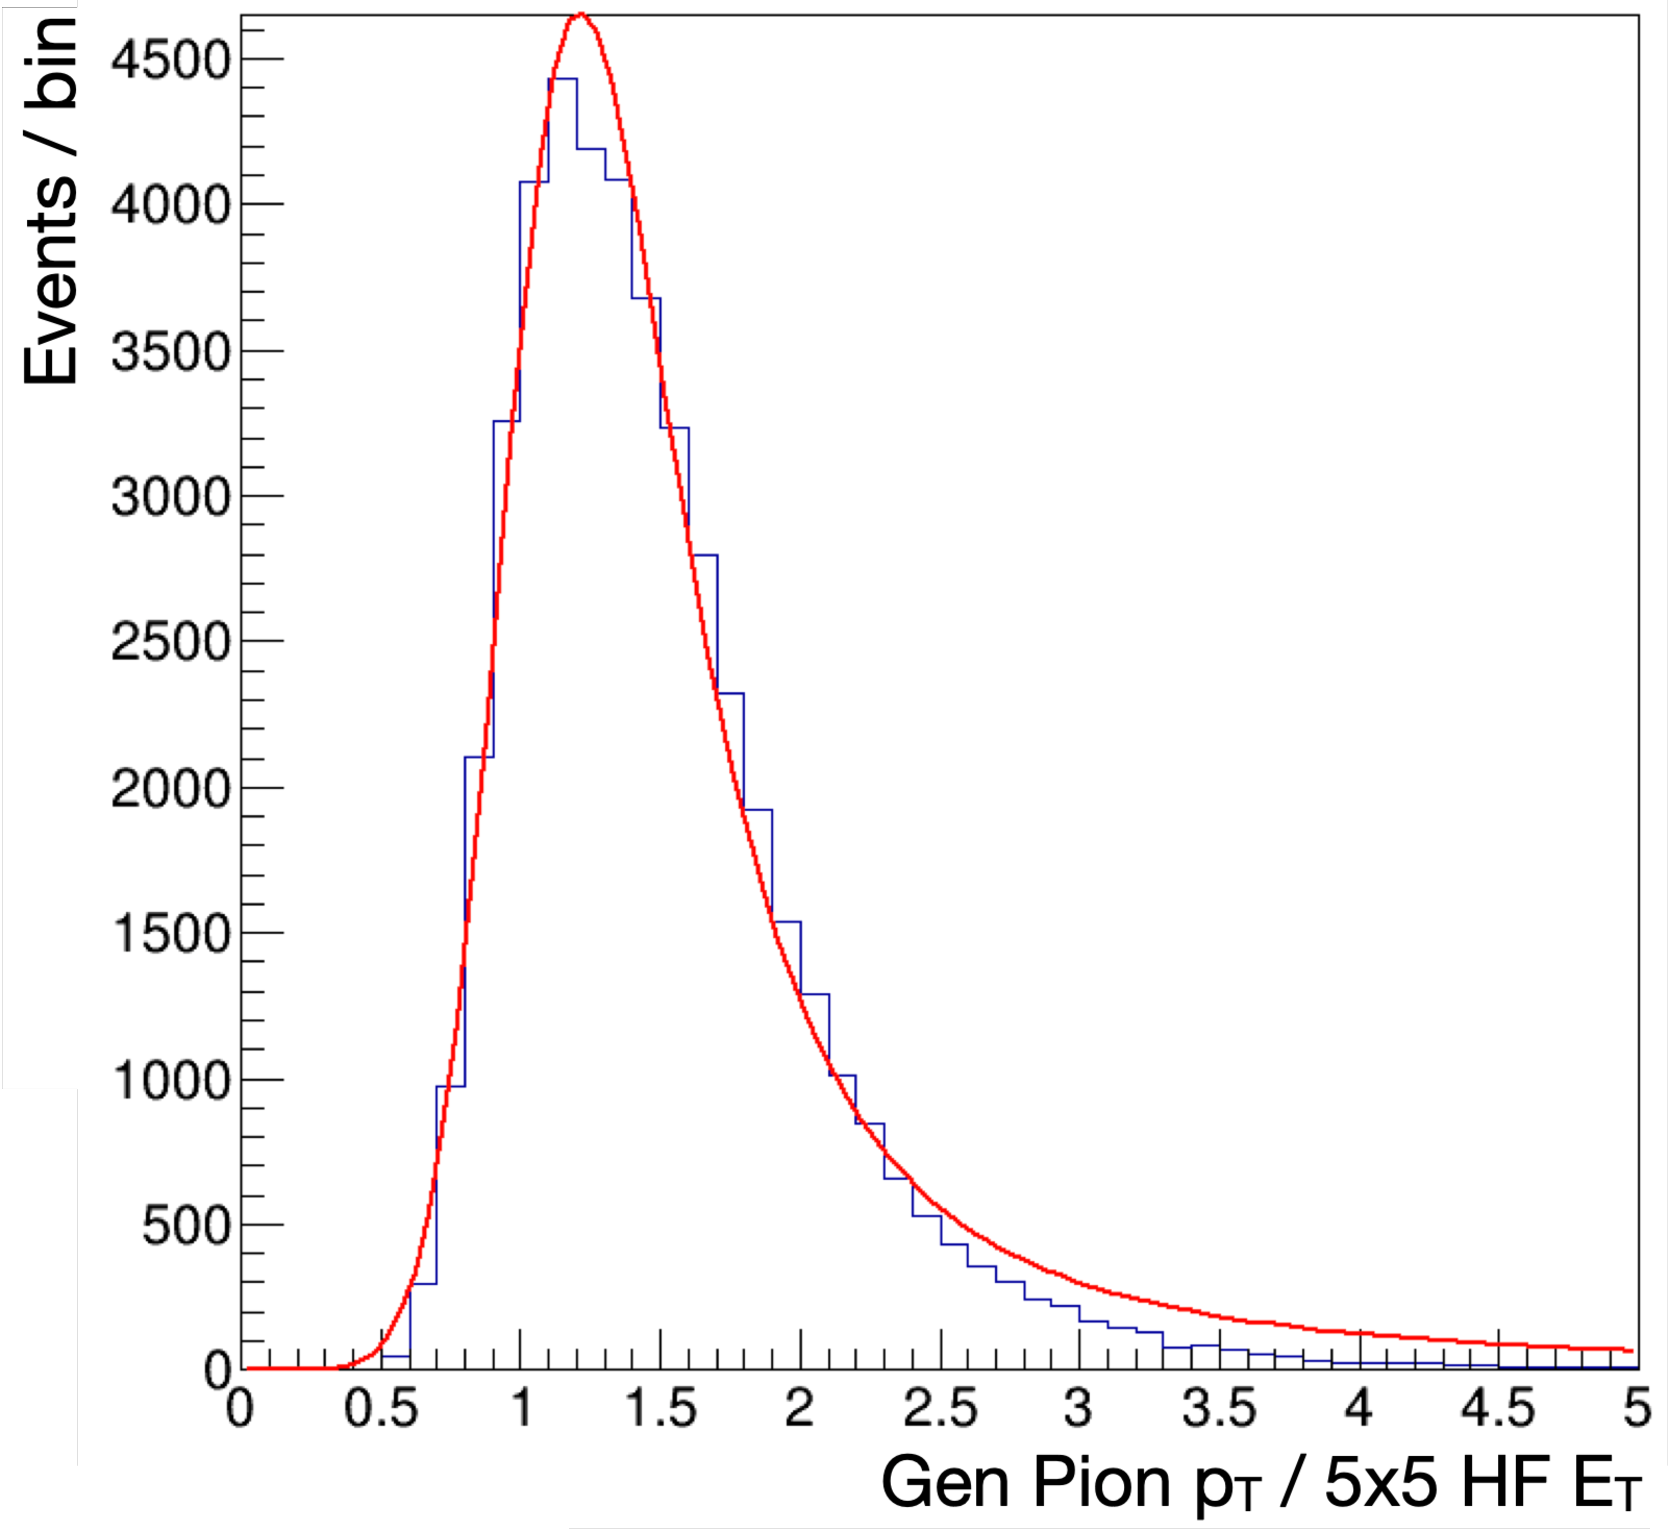
\includegraphics[width=0.4\linewidth]{Figures/L1TP/OldL1HF.pdf}}
    \caption{Distribution of the Layer-1 energy response fitted with a Landau distribution function convoluted with a Gaussian. For ECAL, the response is defined as the ratio between the generated photon transverse momentum and the $3\time3$ $e/\gamma$ cluster energy deposit for $E_T \in [0,3]$~GeV and $i\eta=1$~(a). For HCAL and HF, the response is defined as the ratio between the generated pion transverse momentum and the $5\time5$ jet cluster energy deposit for $E_T \in [0,3]$~GeV and $i\eta=31$~(b).}
    \label{fig:OldL1Fit}
\end{figure}

\begin{figure}
    \centering
    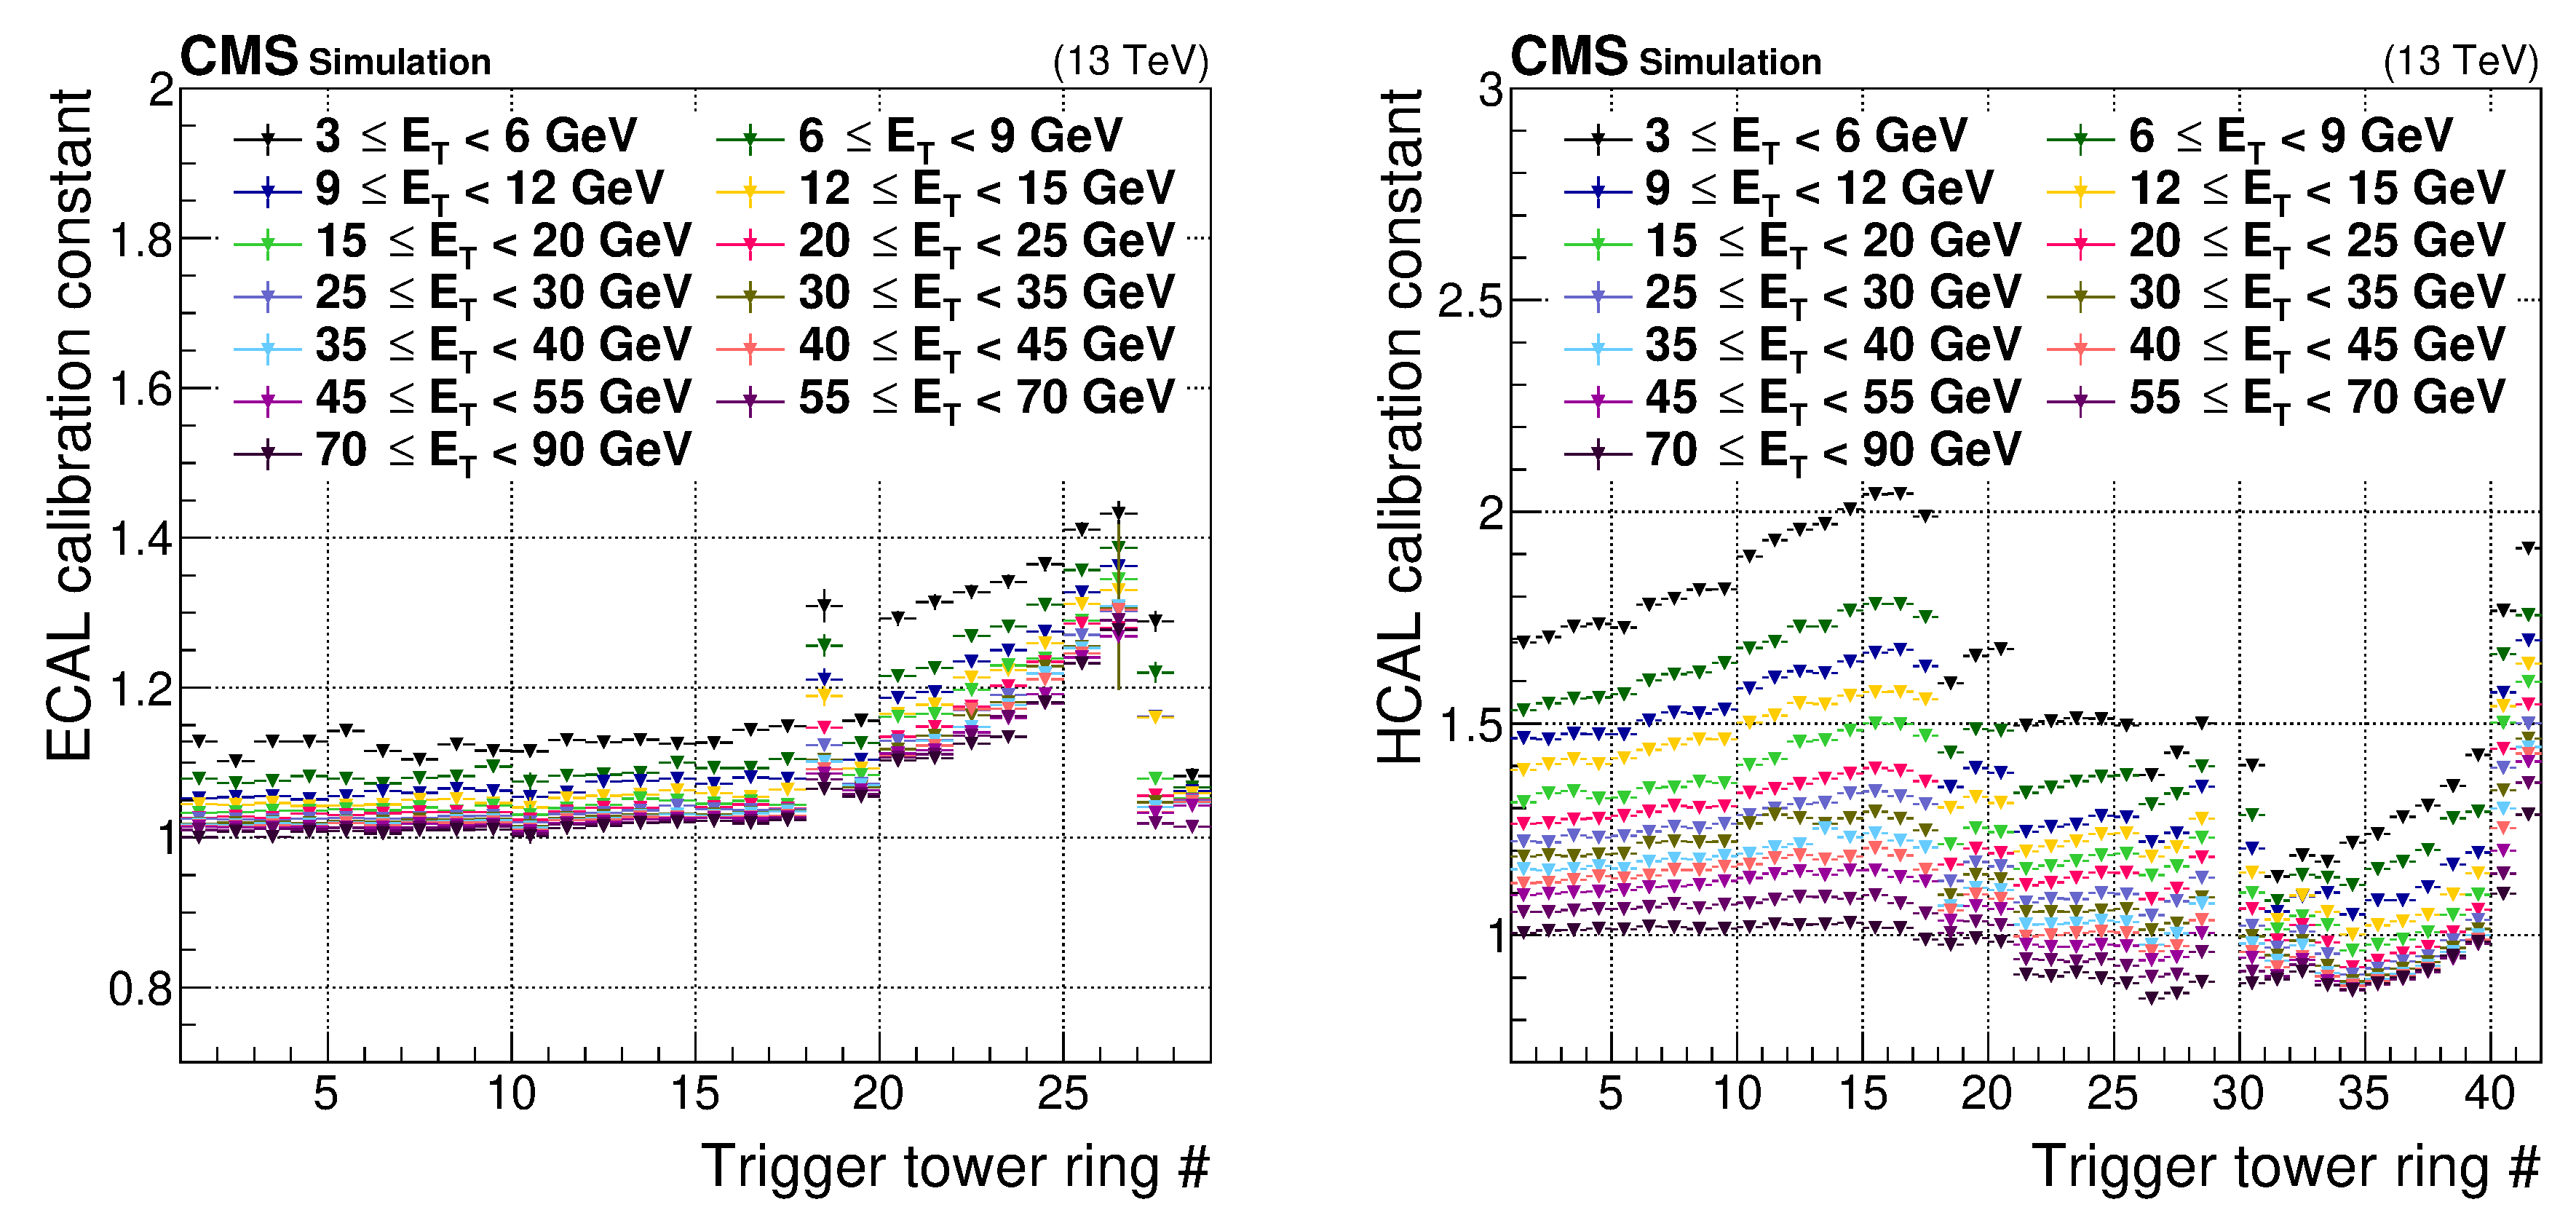
\includegraphics[width=0.9\linewidth]{Figures/L1TP/L1OldSF.pdf}
    \caption{Layer-1 energy scale factors for ECAL (left) and HCAL (right), shown for each constant-$|\eta|$ ring of Trigger Primitives (TP). As specified in the legend, the color of each point corresponds to a range of uncalibrated TP transverse energy values received by the Layer-1 calorimeter trigger. Because of the HCAL geometry, the signals from TPs ring 29 are divided between rings 28 and 30, and no scale factors are applied.}
    \label{fig:L1OldSF}
\end{figure}

\bigbreak

The current method for the extraction of Layer-1 calibration factors has achieved good results throughout Run-II, but suffers from inherent criticality. 
The method is based on the use of MC simulated samples, with particular conditions in terms of flatten energy and $\eta$ distributions, and is affected by its finite statistical power. 
In order to ensure comparable and sufficient statistics in all bins, the approach requires the definition of a small number of coarse energy bins, while the firmware would allow for a finer binning up to one calibration factor every energy digit, i.e. 0.5~GeV.
Moreover, MC samples are based on the simulation of the detector response to generated particles and the simulation of the response in low energy TPs have proven to be not entirely reliable and highly dependent on the continuously varying detector conditions.
Another critical point comes from the definition of the $e/\gamma$ and jet cluster candidates, which does not follow the same algorithm employed in Layer-2; in particular, the HCAL shower can spread beyond the $5\times5$ extension of the cluster.
In addition, once the cluster of multiple TPs has been defined, the calibration factor is only extracted for the central TP through a linear regression. This approach completely ignores any possible dependency on the energy distribution within the cluster or any correlation between different TPs.

These points have become particularly evident at the start of the Run~III data-taking. 
The optimization of ECAL, HCAL, and HF calibrations was performed, but in the case of HCAL and HF, the new correction factors did not pass the necessary validation and closure tests. 
For this reason, for the Run~III data-taking, the choice was made to set HCAL and HF Layer-1 calibration factors to unity, thus removing the needed calibration.

\section{The new Layer-1 calibration method}

A novel ML technique for the detector calibration has been developed for the extraction of Layer-1 calibration factors, aiming to address some of the critical limitations related to the current calibration technique described in the previous section.
This application provides a first proof of concept for the novel ML-based calibration method and offers insights into its potential future applications beyond the L1 Trigger context.

\bigbreak

The primary improvement introduced by the new method stems from the use of ML algorithms to derive calibration constants. Unlike traditional techniques that require the definition of a simplified parametric function to describe the energy response, the ML approach can handle complex, non-linear relationships, which are typically difficult to capture with conventional regression methods. 
ML models can learn from large amount of data simultaneously and interpolate the detector response even for objects that were not included in the training dataset.
Moreover, the capability of ML methods to incorporate multiple input variables allows for a faster extrapolation of the calibration constants, without necessitating finite, coarse energy bins. However, in this specific application, the calibration factors are constrained by firmware compatibility, necessitating a minimum energy bin size of $\Delta E_T\geq0.5$~GeV.

The second improvement comes from a redefinition of the clusters defining the $e/\gamma$ and jet candidates. 
According to the Layer-2 conventions for the hadronic jet candidates, the L1 cluster is defined, both for $e/\gamma$ and jet objects, as the $9\times9$ matrix of TTs composing the \textit{chunky donut} (CD). This choice ensures maximal containment of the hadronic shower, and minimal energy loss. This inclusive definition of the L1 cluster has revealed itself as a convenient approach for the calibration of jets, whilst the $e/\gamma$ cluster, initially defined as the same $9\times9$ TTs CD shape, has been subsequently revised to a smaller shape, in order to reduce the contamination from pile-up. 
In the new method, no requirements are applied to the energy deposit in the central TP, allowing for different candidate shapes to enter the calibration process, expanding the effectiveness of the calibration to account for a wider range of possible shapes.

Finally, the method described in this Chapter is based on the possibility of extracting the calibration factors using either MC simulated events or data. In the first case, the calibration method benefits from a better definition of the true object energy at generator level, and from the simulation of the ideal environment of no pile-up, hardly achievable during ordinary data taking conditions. In the latter, the use of data presents more arduous conditions due to the inevitable contribution of pile-up, however it provides the most reliable representation of the latest detector response, with continuously increasing training datasets as more data becomes available.
The design and optimisation of the method is performed based on data collected by the CMS Experiment, with two separate samples for the derivation of the ECAL and HCAL/HF calibration constants.
For the derivation of the ECAL calibration factor, the \texttt{EGamma} dataset is used, which is composed of events triggered by HLT paths requiring the presence of electron or photon candidates. For the derivation of the HCAL/HF calibration, the \texttt{JetMET} dataset is used, which is recorded by requiring the presence of jet or missing transverse energy candidates.

% \bigbreak

% The first implementation of the new Layer-1 calibration method was based on a Neural Network (NN) approach~\cite{Motta:2881939}, which I contributed in developing and optimising. This initial attempt is discussed in Section~\ref{sec:The Neural Network approach}, however it was found to have intrinsic limitations for the specific application of the calibration to the Layer-1 context. 
% As part of this Thesis work, I have converted the NN method into a new algorithm based on differentiable programming, allowing for streamlined parameter optimisation and customisation of the Layer-1 calibration constants for a better compatibility with the Layer-2 requirements.

% The Trigger Primitives that used to build the Level-1 Trigger calorimeter objects (electron, photon, tau leptons, jets, etc.) are calibrated using the method described in Ref. \cite{CMS:2020cmk}. It consists in deriving calibration factors for the ECAL and Hadronic Calorimeter (HCAL) from single-photon (single-pions)
% simulations. The calibration factors are extracted, in bins of $\eta$ and transverse energy, from the distribution of the calorimeter response, i.e. the ratio of the true particle energy (a photon or a pion) to the energy of a group of 3 (9) Trigger Primitives.\\

\section{The Neural Network approach}
\label{sec:The Neural Network approach}

The first implementation of the new method for the extraction of Layer-1 calibration factors is based on a NN approach, which I contributed in developing and optimising.
The idea behind this first implementation is to exploit innovative and widely employed software techniques to bypass the drawbacks of the standard linear regression method, taking advantage of the ability of NNs to model complex, non-linear relationships and to efficiently handle large datasets.
Moreover, the NN approach entirely removes the need for arbitrary choice of energy binning to perform fits and can learn about possible correlations between the different TTs composing the L1 candidate.

The input to the NN is the raw energy deposit $E_T$ and $i\eta$ position of each TT composing the $9\times9$ L1 candidate.
The goal of the NN approach is learning to predict the best calibration factors to be applied to each TT so that the calibrated L1 energy is as close as possible to the reference value, defined as the energy of the reconstructed object:

\begin{equation}
    E_T^{\,L1,\;jet} = \sum_{i\eta,\:i\phi}\left(\;\alpha\,(i\eta,E_{T})\;\cdot\;E_{T}\;\right) 
    \;\longrightarrow\;
    E_T^{\:Reco,\;jet}
\label{eq:Training}
\end{equation}
where $E_T^{\,L1,\;jet}$ is the calibrated L1 energy, $\alpha\,(i\eta,E_{T})$ are the calibration factors, depending on the $E_T$ energy deposit and $i\eta$ position of the TT, and $E_T^{\:Reco,\;jet}$ is the energy of the reconstructed object.

\subsection{Basic concepts of Neural Networks}

The main idea behind NNs is reproducing the neuronal organisation found in animal brains through software implementations~\cite{1672070}.
The structural building blocks of NNs are artificial neurons, also known as \textit{perceptrons}, taking as input $n$-dimensional vectors of variables $(x_1,x_2,...,x_n)$. Each variable is multiplied by a different weight $w_i$ and summed together, adding a bias term $b$.
The outcome of the summation is then fed into an activation function $f$, which can be either linear or non-linear, the latter option generally being preferred as the introduction of non-linearity enables the NN to capture arbitrarily complex relationships in data.
Mathematically, each artificial neuron can be represented as a unit performing the following operation:
\begin{equation}
    \hat{y}=f\left( \sum_{i=1}^{n}w_i \cdot x_i + b \right)
\end{equation}
where $\hat{y}$ represents the output of the neuron, and the process of feeding the inputs to a neuron is known as \textit{forward propagation}. A graphical illustration of the neuron can be found in Figure~\ref{fig:Perceptron}.

\begin{figure}
    \centering
    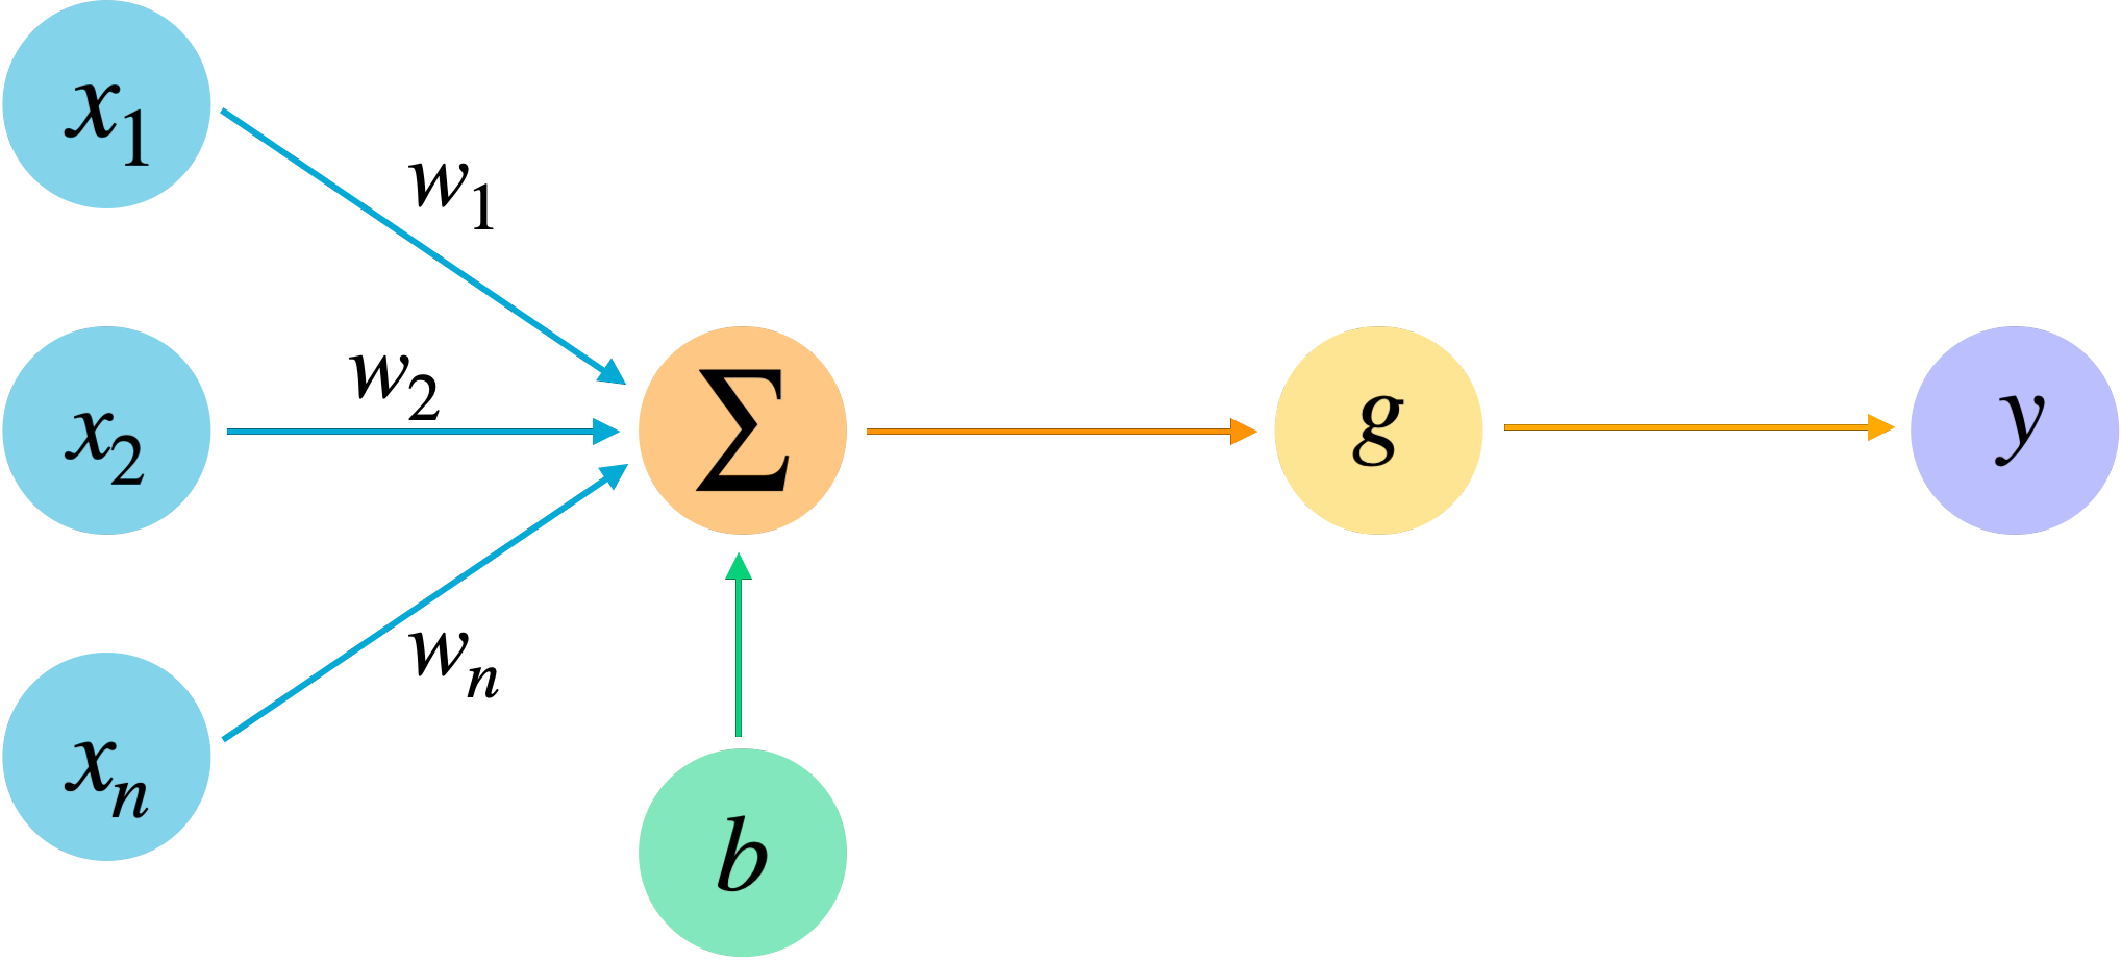
\includegraphics[width=0.6\linewidth]{Figures/L1TP/Perceptron.pdf}
    \caption{Graphic illustration of an artificial neuron. An $n$-dimensional vector of variables is passed as input, and weights are applied to each element. The weighted vector is summed and added to a bias term, the sum is passed to a non-linear activation function $f$, which returns the output $y$.}
    \label{fig:Perceptron}
\end{figure}

In a typical NN architecture, neurons are arranged into layers, and each neuron in a layer receives inputs from the neurons in the preceding layer. 
The structure of the NN is fully defined by the configuration of these layers and the number of neurons in each layer. A typical NN includes an input layer, multiple hidden layers, and an output layer, as illustrated in Figure~\ref{fig:Architecture}.
% The output layer can produce one or multiple output values, depending on the specific problem being addressed. 
At this stage, the NN is simply a sequence of neurons, taking as input a set of variables, and computing mathematical operations to generate the output. The degree of complexity of the NN function is directly related to its architecture: at a first approximation, the number of layers corresponds to the degree of the polynomial functions, while the number of neurons in each layer regulates the monomials of the same degree. 

Once the NN architecture is defined, the goal is to adjust the NN weights in such a way that the prediction for the final output $\hat{y}$ is as close as possible to the truth value. 
In order to quantify the discrepancy between the NN prediction and the real quantities, different metrics can be adopted, generally referred to as \textit{loss functions}:
\begin{equation}
    L(w,b)=\frac{1}{N}\sum_{j=1}^N(y_j-\hat{y}_j)^2
\end{equation}
where $N$ is the number of input samples, $y_i$ is the truth value being learnt, and $\hat{y}_i$ is the predicted NN output.
The minimization of the loss function, also known as \textit{training}, is achieved by feeding the NN with a dataset where the truth value $y_i$ of the target variables are already known.
During the training process, the loss function is derived with respect to the weights, and the trainable parameters are progressively updated in the opposite direction to the gradient, thus guiding the NN weights to values that minimise the loss. The procedure of updating the weights following the loss gradient is usually referred to as \textit{backward propagation}, and can be tuned by a learning rate parameter defining the magnitude of the parameter variation during each training iteration. A small learning rate leads to slow convergence and risks getting the NN trapped in local minima, whereas a large learning rate can cause the process to overshoot the optimal weights, resulting in instability and divergence.

After initialising the weights to random values, the process of training a NN model is constituted by an iterative repetition of the following steps, until convergence:
\begin{itemize}
    \item Evaluate the loss function with the current set of weights, $W$ (\textit{forward propagation});
    \item Compute the gradient of the loss function with respect to the set of weights, $\partial L/\partial W$;
    \item Update the weights in the opposite direction to the gradient, with a step proportional to the learning rate, $W = W - (\partial L/\partial W \times LR)$ (\textit{backward propagation}).
\end{itemize}
A schematic overview of a typical NN architecture and its training process is reported in Figure~\ref{fig:Architecture}.

\begin{figure}
    \centering
    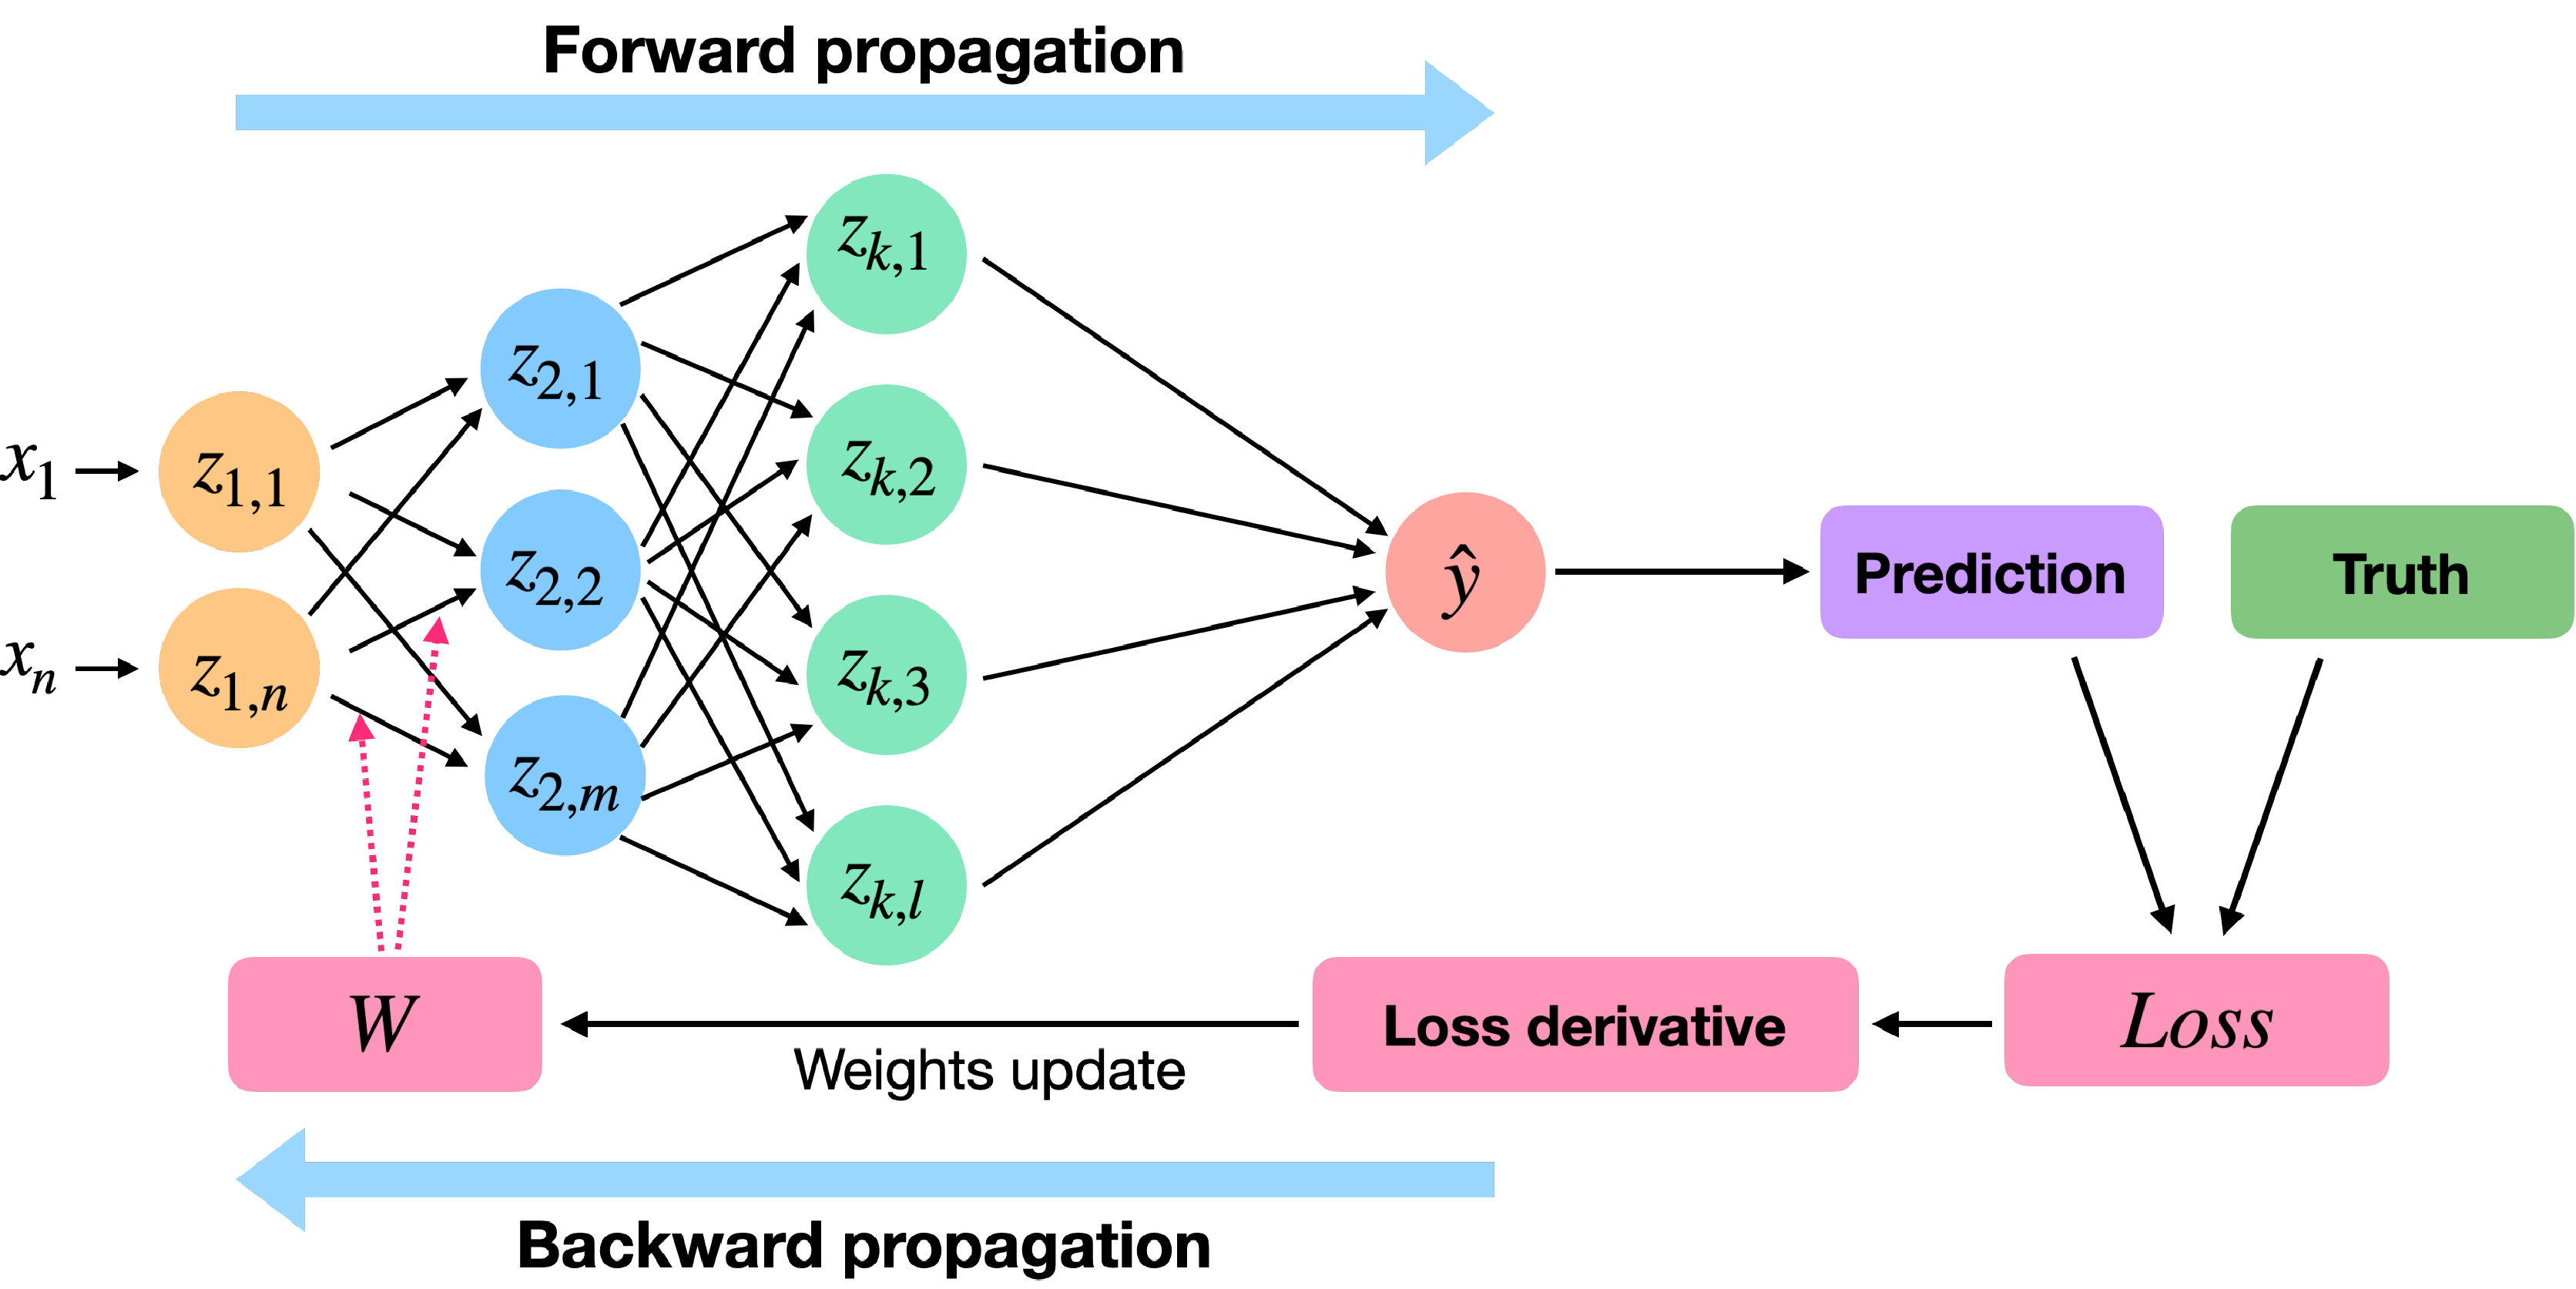
\includegraphics[width=0.8\linewidth]{Figures/L1TP/Architecture.pdf}
    \caption{Schematic representation of a typical Neural Network (NN) architecture, alongside its basic training steps. The input data is fed to the NN, which processes it in the forward propagation to give a prediction; the loss function is computed, encoding the discrepancy between prediction and truth values; in the backward propagation, the loss is derived and the trainable parameters are updated according to an optimizer that minimizes the loss function.}
    \label{fig:Architecture}
\end{figure}

% \subsection{Input definition}
% In the new ML-based method, the L1 objects are defined as a $9\times9$ matrix of TTs, and the Layer-1 raw energy of each candidate is defined as the sum of the $iE_T$ energy deposit in the 

\subsection{The algorithm architecture and training procedure} 

The NN designed for the Layer-1 TTs calibration is based on a custom architecture, in order to handle the input features coming from the position and raw energy of the TTs composing the $9\times9$ CD, and extract the predicted calibrated energy of the L1 candidate.

% architecture
A schematics of the NN architecture is reported in Figure~\ref{fig:TTP}.
The basic building block of the NN architecture is the Trigger Tower Predictor (TTP), a stand-alone network, which takes as input the energy deposit and $i\eta$ position of a single TT and extracts the predicted calibrated TT energy.
The TTP is structured as a fully connected layer with 84 neurons, a hidden layer with 256 neurons, and one single-neuron output layer. All neurons make use of the Rectified Linear Unit (ReLU)~\cite{4082265} activation function, and the bias parameter is inhibited in order to avoid propagating the information of empty TTs.
In order to simulate the Layer-1 firmware algorithm, which is based on the transmission of 8-bit words with discrete values for TT the energy deposit, a custom layer is applied to the output of the TTP, flooring the output of the previous layer in units of $iET$ (i.e. 0.5~GeV precision).
The TTP is cloned 81 times, to reproduce the $9\times9$ array of TTs, with each clone sharing the same trainable parameters.
The outputs of the 81 TTP clones are then summed together in a non-trainable \textit{summation layer}, to obtain the predicted calibrated L1 candidate energy.

\bigbreak

\begin{figure}
    \centering
    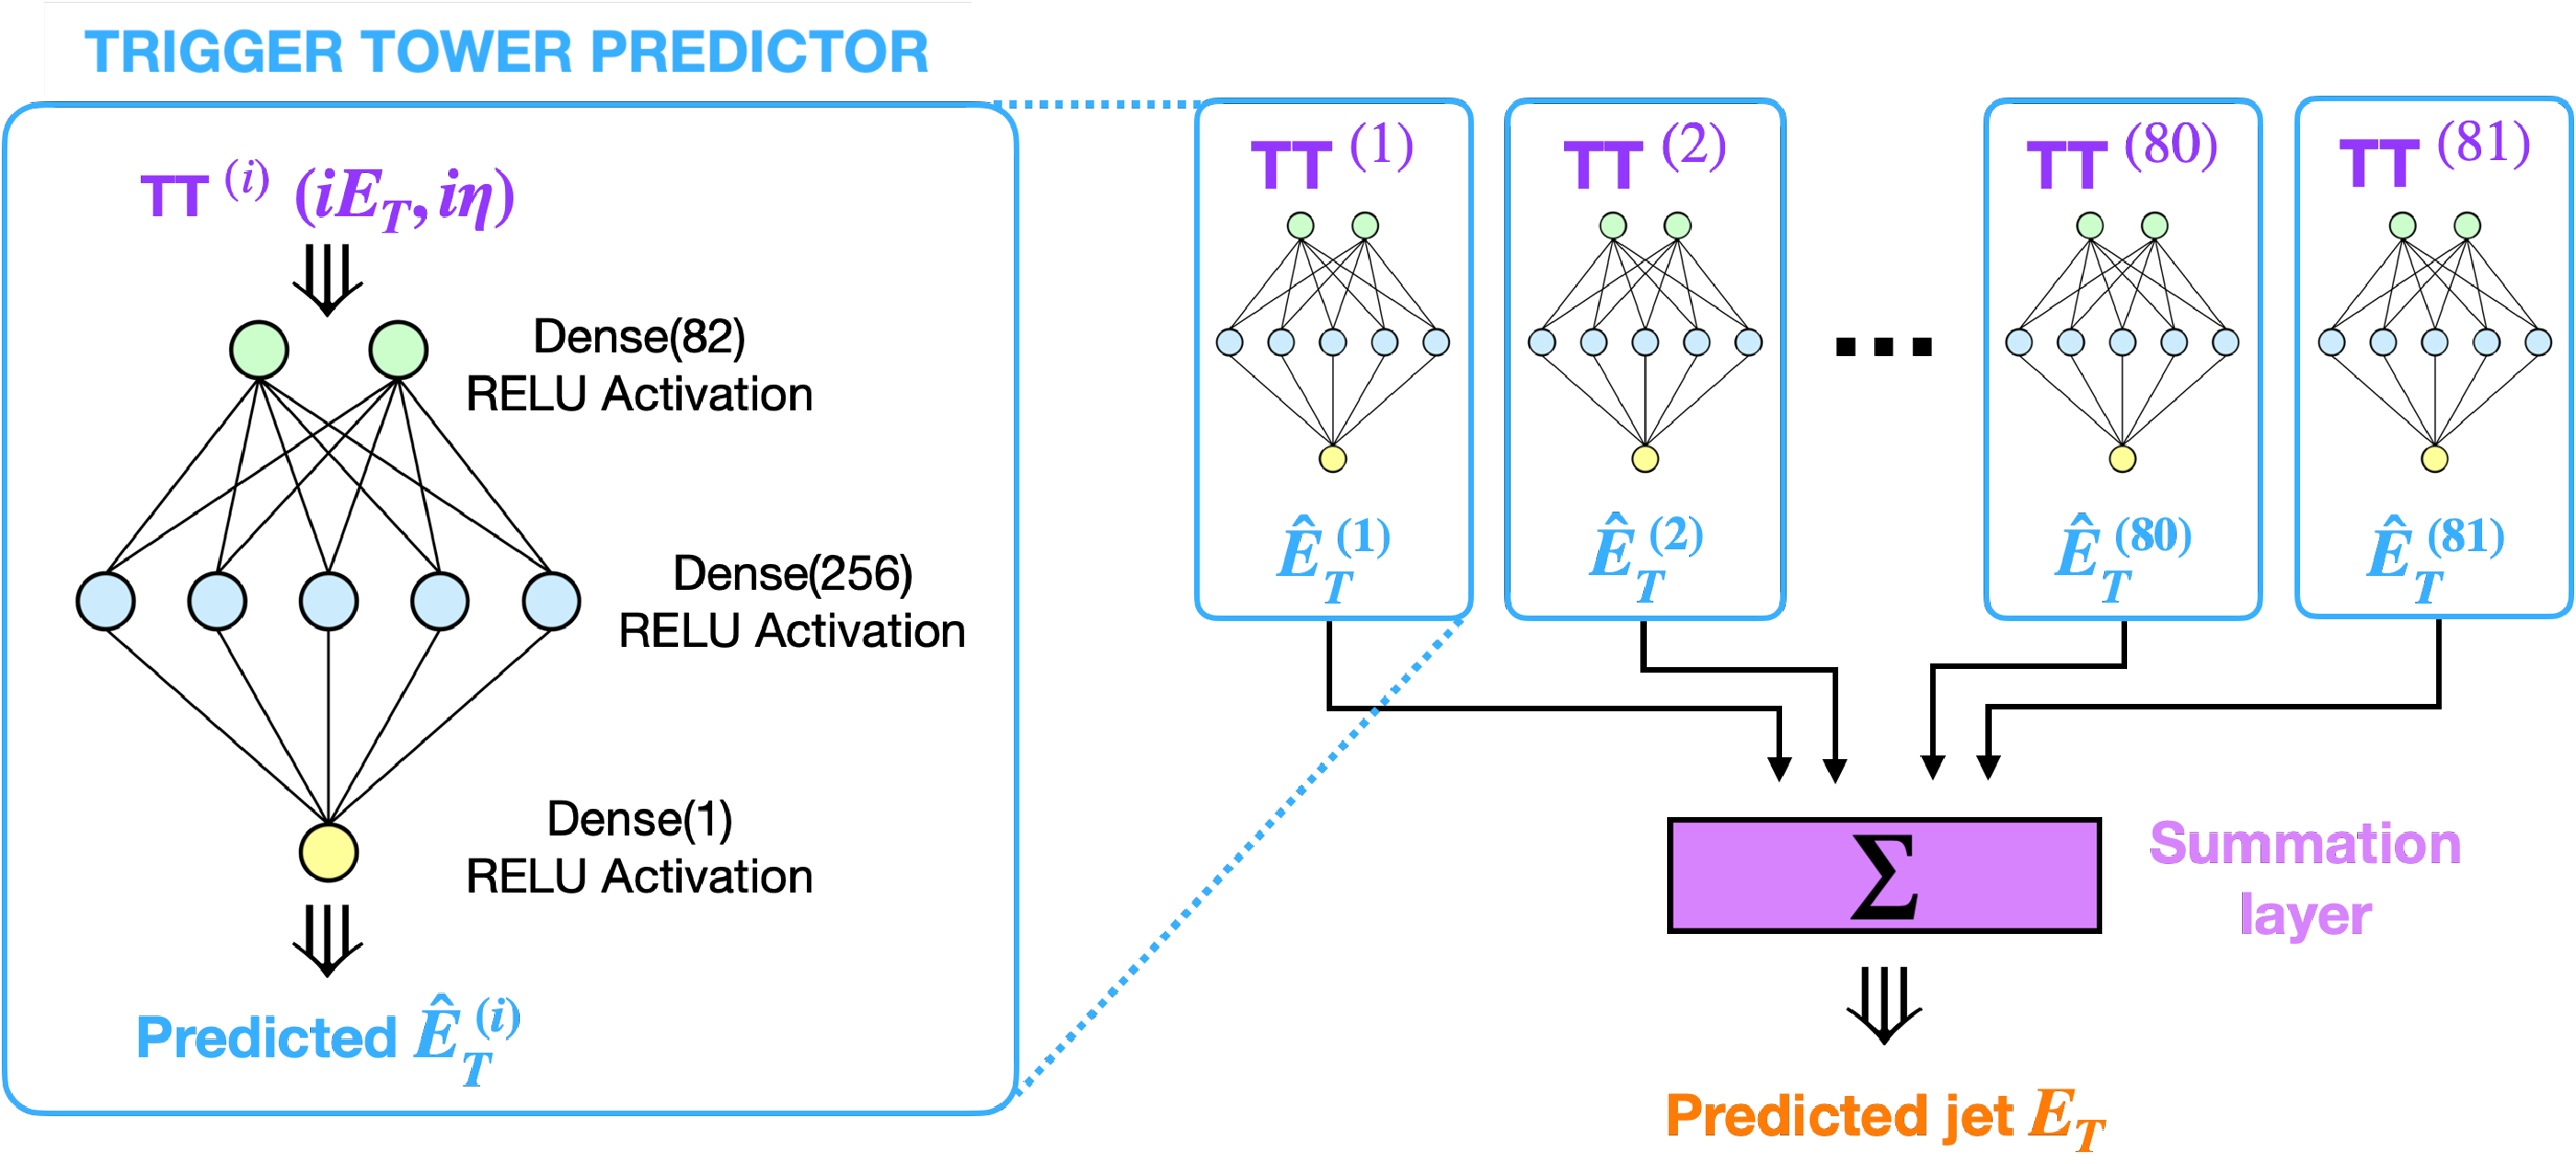
\includegraphics[width=0.8\linewidth]{Figures/L1TP/TTP.pdf}
    \caption{Schematic view of the NN architecture. The basic component is the Trigger Tower Predictor (TTP), a stand-alone NN, which takes as input the energy deposit and $i\eta$ position of a single TT and extracts the predicted calibrated TT energy. The TTP is cloned 81 times, and the outputs are summed together in the summation layer, to extract the predicted calibrated L1 candidate energy.}
    \label{fig:TTP}
\end{figure}

% Training
Once the NN architecture has been defined, the training is performed by minimising a custom loss function, containing three different terms:
\begin{itemize}
    \item \textit{Regression term}: it evaluates the distance between the predicted L1 calibrated energy, at the output from the summation layer, and the target offline energy of the matched object, by using the Mean Absolute Percentage Error (MAPE) function.
    \item \textit{Regularisation term}: it is computed as the squared sum of all the network’s weights and maintains the trainable parameters small, in order to avoid neuron subset over-training.
    \item \textit{Rate term}: it is a penalty term based on the evaluation of the L1 rate proxy, with the effect of maintaining the estimated L1 rate close to the current level.
\end{itemize}
Each term is regulated by a multiplication factor, considered as a NN \textit{hyper-parameter}, that can be varied to adjust the relative importance of each term to optimise the NN performance. The loss function is mathematically expressed as:
\begin{equation}
L = 
A\cdot\left|\frac{E_T^{L1,\;jet} - E_T^{Reco,\;jet}}{E_T^{Reco,\;jet}}\right|
\;+\;
B\cdot\sum_iw_i^2
\;+\;
C\cdot\cosh\left(D\cdot\frac{R_{proxy} - R_{target}}{R_{target}}\:\right)
\end{equation}
where $E_T^{\:L1,\;jet}$ and $E_T^{\:Reco,\;jet}$ are the energy of the calibrated L1 candidate and of the offline object respectively, $w_i$ is the NN trainable parameter, and $R_{target}$ and $R_{proxy}$ are the estimate for the rate proxy obtained by applying either the current or the newly trained Layer-1 calibration factors.

The rate term was introduced at a second iteration of the NN architecture implementation, to cope with L1 trigger rate increase. In principle, a better calibration of Layer-1 TTs translates in a more precise application of energy thresholds, and a better management of the final rate; however, with the sole information of the TTs raw energy deposit, it is hard to correctly discriminate the energy contribution coming from pile-up, and a good calibration of physics objects also tends to enhance the energy of pile-up jets, causing a steep rise in the L1 trigger rate.
The structure of the NN was modified in such a way to receive as input at the same time the L1 candidates from electron an jet signals, and the L1 candidates from zero bias events, the former being employed for the energy regression of the offline objects $E_T$ and the latter for evaluating a rate proxy $R$.
The rate proxy is estimated for jets as the ratio of $9\times9$ CD candidates with a total calibrated energy above 50~GeV, while for $e/\gamma$ it is given by the number of candidates with a recorded seed energy deposit larger than 25~GeV and $H/E$ energy fraction smaller than $2^{-3}$ or $2^{-4}$ for barrel and endcap respectively:
\begin{equation}
    R_{jet} = \frac{\#~\textnormal{Jets with }E_T^{L1,\;jet} > 50~\textnormal{GeV}}{\#~\textnormal{Jets}}
\end{equation}
\begin{equation}
    R_{e/\gamma} = \frac{\#~e/\gamma~\textnormal{having seed with }E_T > 25~\textnormal{GeV}~\&~H/E < 2^{-3(-4)}}{\#~e/\gamma}
\end{equation}
Given the large size of low energy L1 candidates in the zero-bias dataset, the input for the rate proxy estimation is preliminarily reduced by applying a cut on the transverse momentum of the offline objects matched to the L1 candidate, requiring $p_T>15$~GeV for both $e/\gamma$ and jets.
To further accelerate the training time, the training is distributed on four NVIDIA Tesla V100 Tensor Core GPUs~\cite{NVIDIAgpu}. 
% problem with the rate: the input is preselected, but there might be new clusters appearing as we increase the SFs

\bigbreak

Two separate training procedures are performed to extract ECAL and HCAL calibration factors. For the ECAL Layer-1 calibration factors, the training dataset is composed of electrons originating from the Z boson decay, satisfying the requirement $|\eta| < 3.0$, and having an electromagnetic energy deposit fraction larger than $95\%$.
For the HCAL Layer-1 calibration factors, the training dataset is composed of jets identified with the PileUp Per Particle (PUPPI) algorithm~\cite{PUPPI_2014}, having pseudorapidity value $|\eta| < 5.1$, transverse momentum $p_T>30$~GeV, and a hadronic energy deposit fraction larger than $80\%$.
In both cases, the $9\times9$ CD matrix is built around the TT with the smallest angular distance from the offline reconstructed object, and only the events having an uncalibrated response close to unity are selected:
\begin{equation}
    0.3 < \frac{E_T^{L1,\;jet}}{E_T^{L1,\;Reco}} < 3.0
\end{equation}
to prevent the NN from learning features of a small fraction of problematic outliers.
The input dataset is divided into training (80\%) and testing (20\%) datasets, to control the potential overfitting of the model.
An \textit{Adam} minimiser~\cite{ADAM_2017} with $10^{-3}$ learning rate is chosen for the NN training.

% To ensure that the $i\eta$ coordinate is interpreted as a discrete variable, a categorical \textit{one-hot encoding} is performed: this technique converts a discrete quantity into a binary vector, with a length equal to the number of unique values, in this case the 41 $i\eta$ positions, which is filled with 0 in each position, except for only single bit stored to 1 corresponding to the specific value of the quantity.

\subsection{Calibration factors and Layer-1 performance}

% Scale factors extraction
The calibration factors are extracted through a \textit{standard candle} approach, by inputting to the trained TTP a standard candle TT, with fixed energy and position. The calibration factor is defined as the ratio between the predicted tower energy and the input raw energy:
\begin{equation}
    \alpha\,(i\eta,E_{T}) = \frac{i\hat{E}_T}{iE_T} = \frac{\textnormal{TTP}(i\eta,iE_T)}{iE_T}
\end{equation}
where $i\eta$ and $iE_T$ are the position and energy deposit of the standard candle TT, and $i\hat{E}_T$ is the TT energy deposit predicted by the TTP.
While the choice for the $i\eta$ position binning is fixed by the detector geometry, the choice for the energy binning is arbitrary, since the NN does not assume any binning or discreteness in the energy by construction. 

\begin{figure}
    \centering
    \subfloat[Current method (ECAL)]{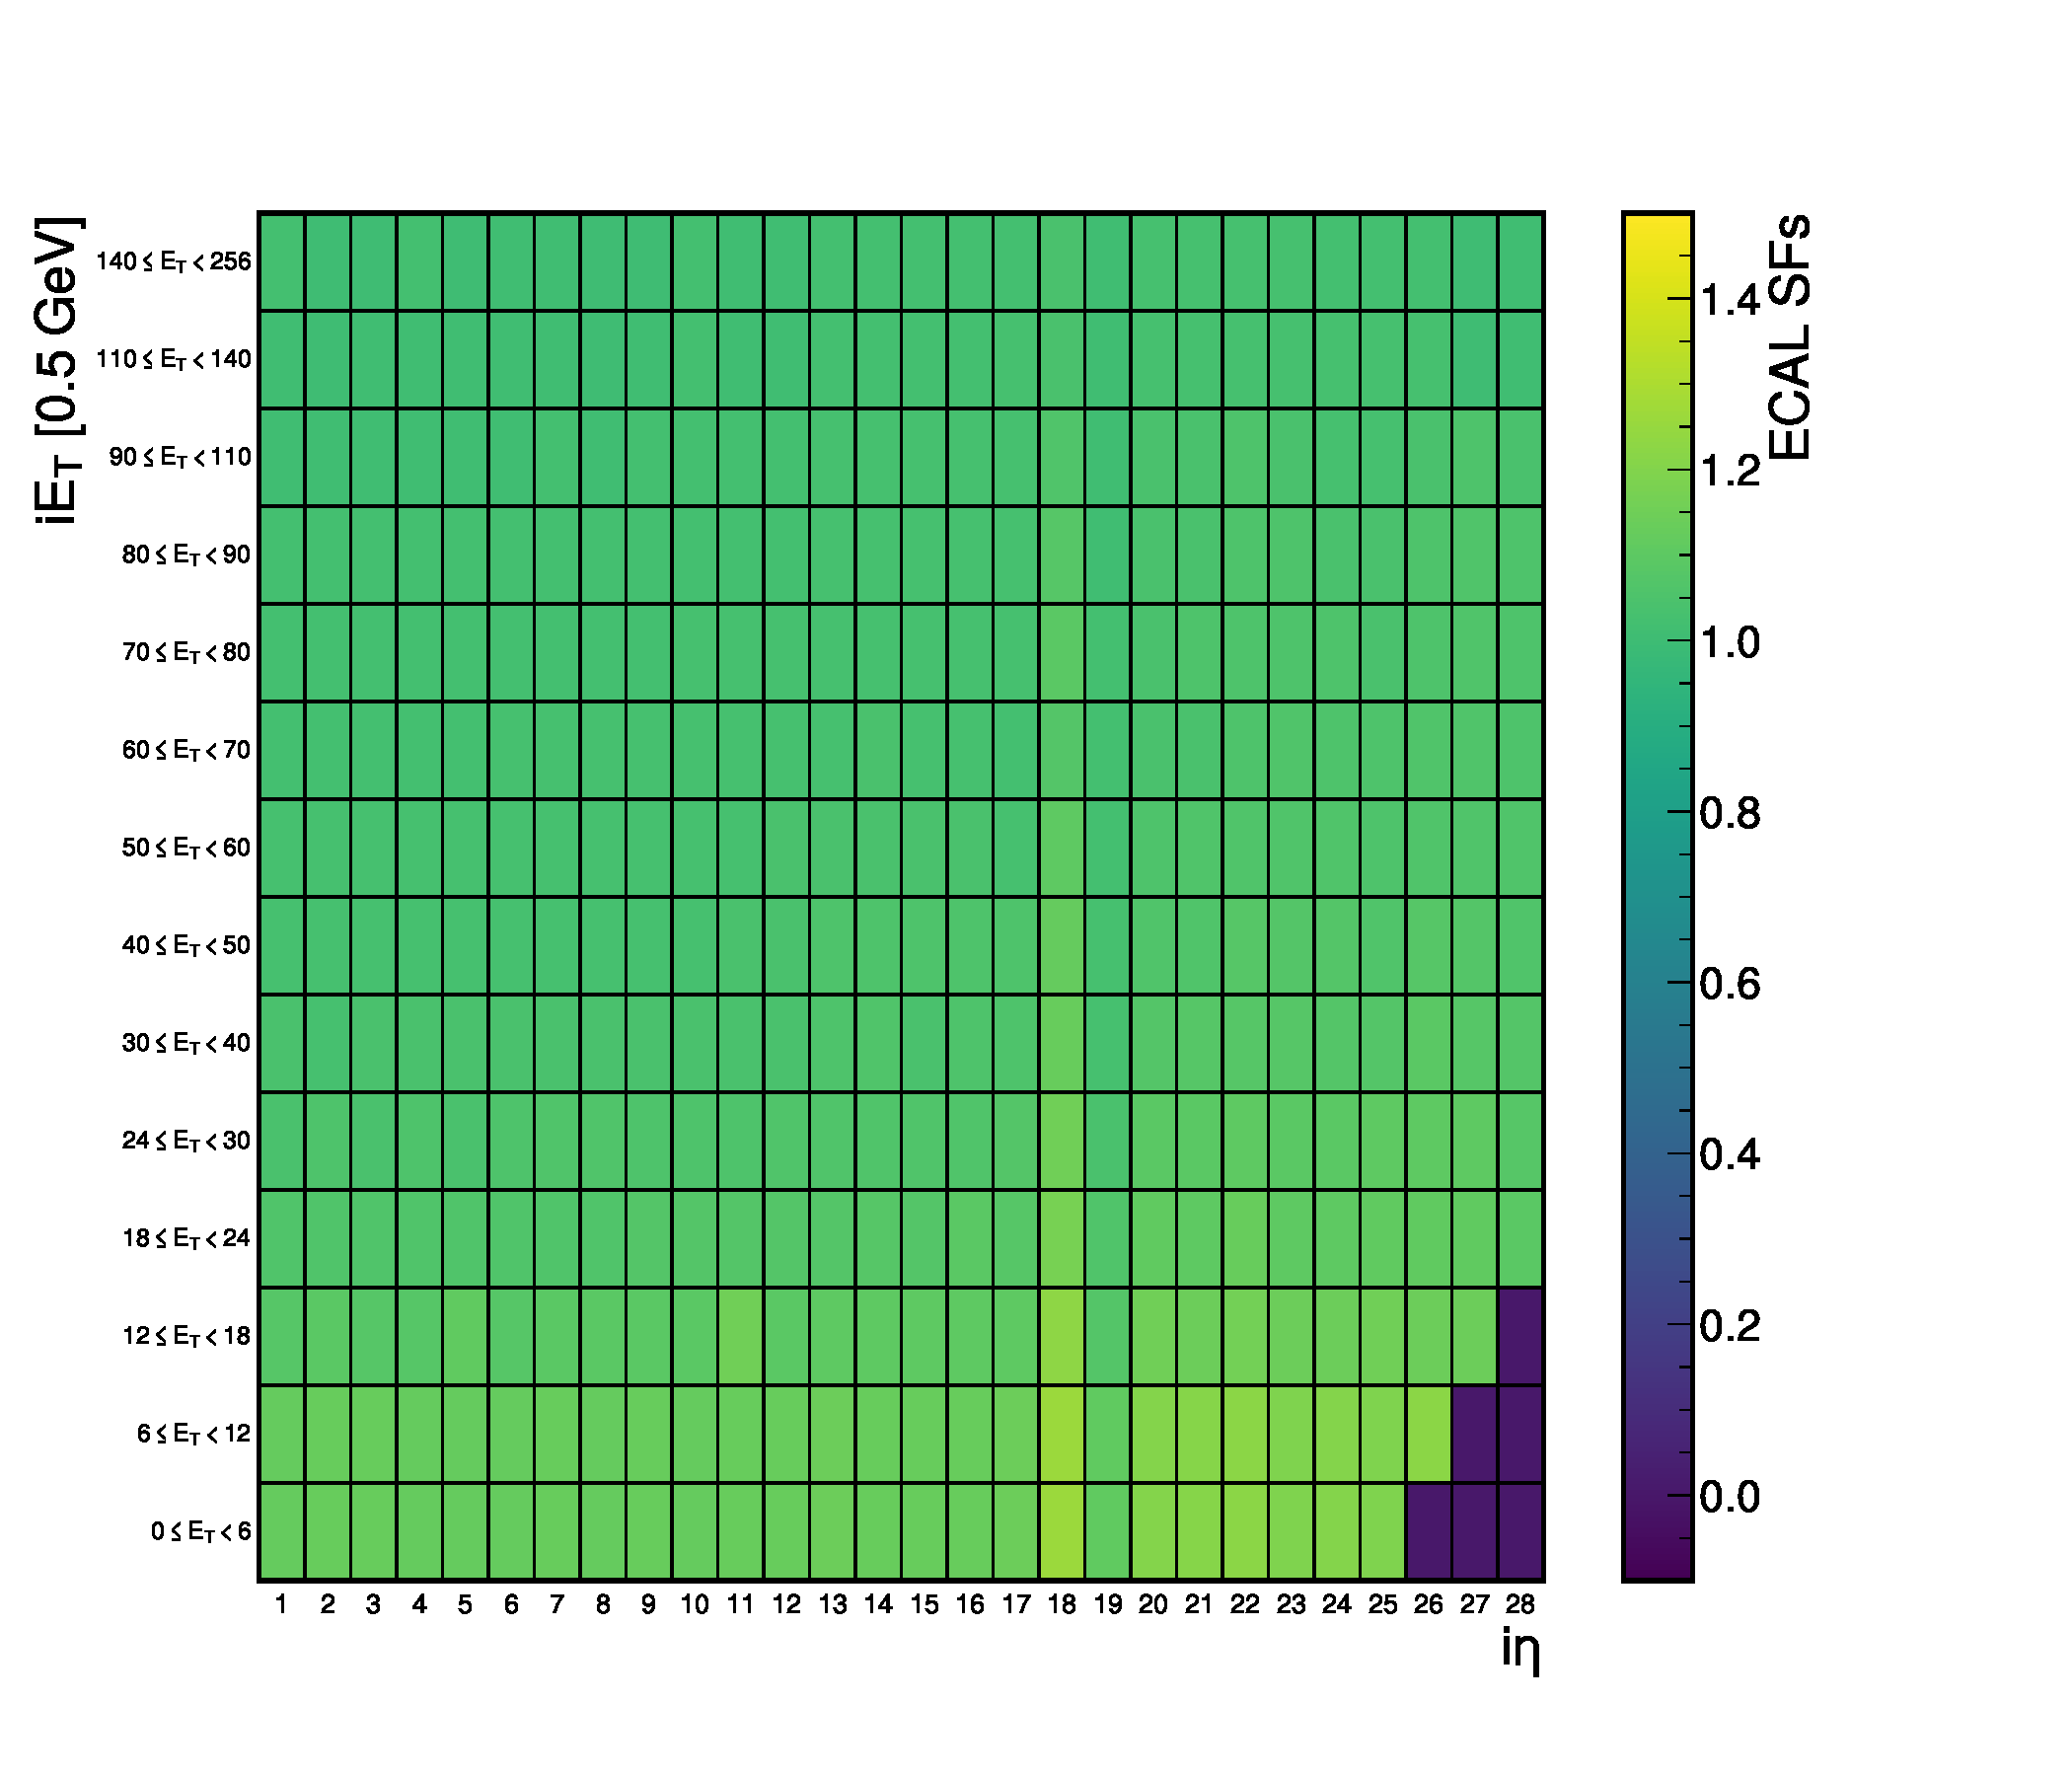
\includegraphics[width=0.5\linewidth]{Figures/L1TP/SFs_2D_ECAL_Thesis.pdf}}
    \subfloat[NN method (ECAL)]{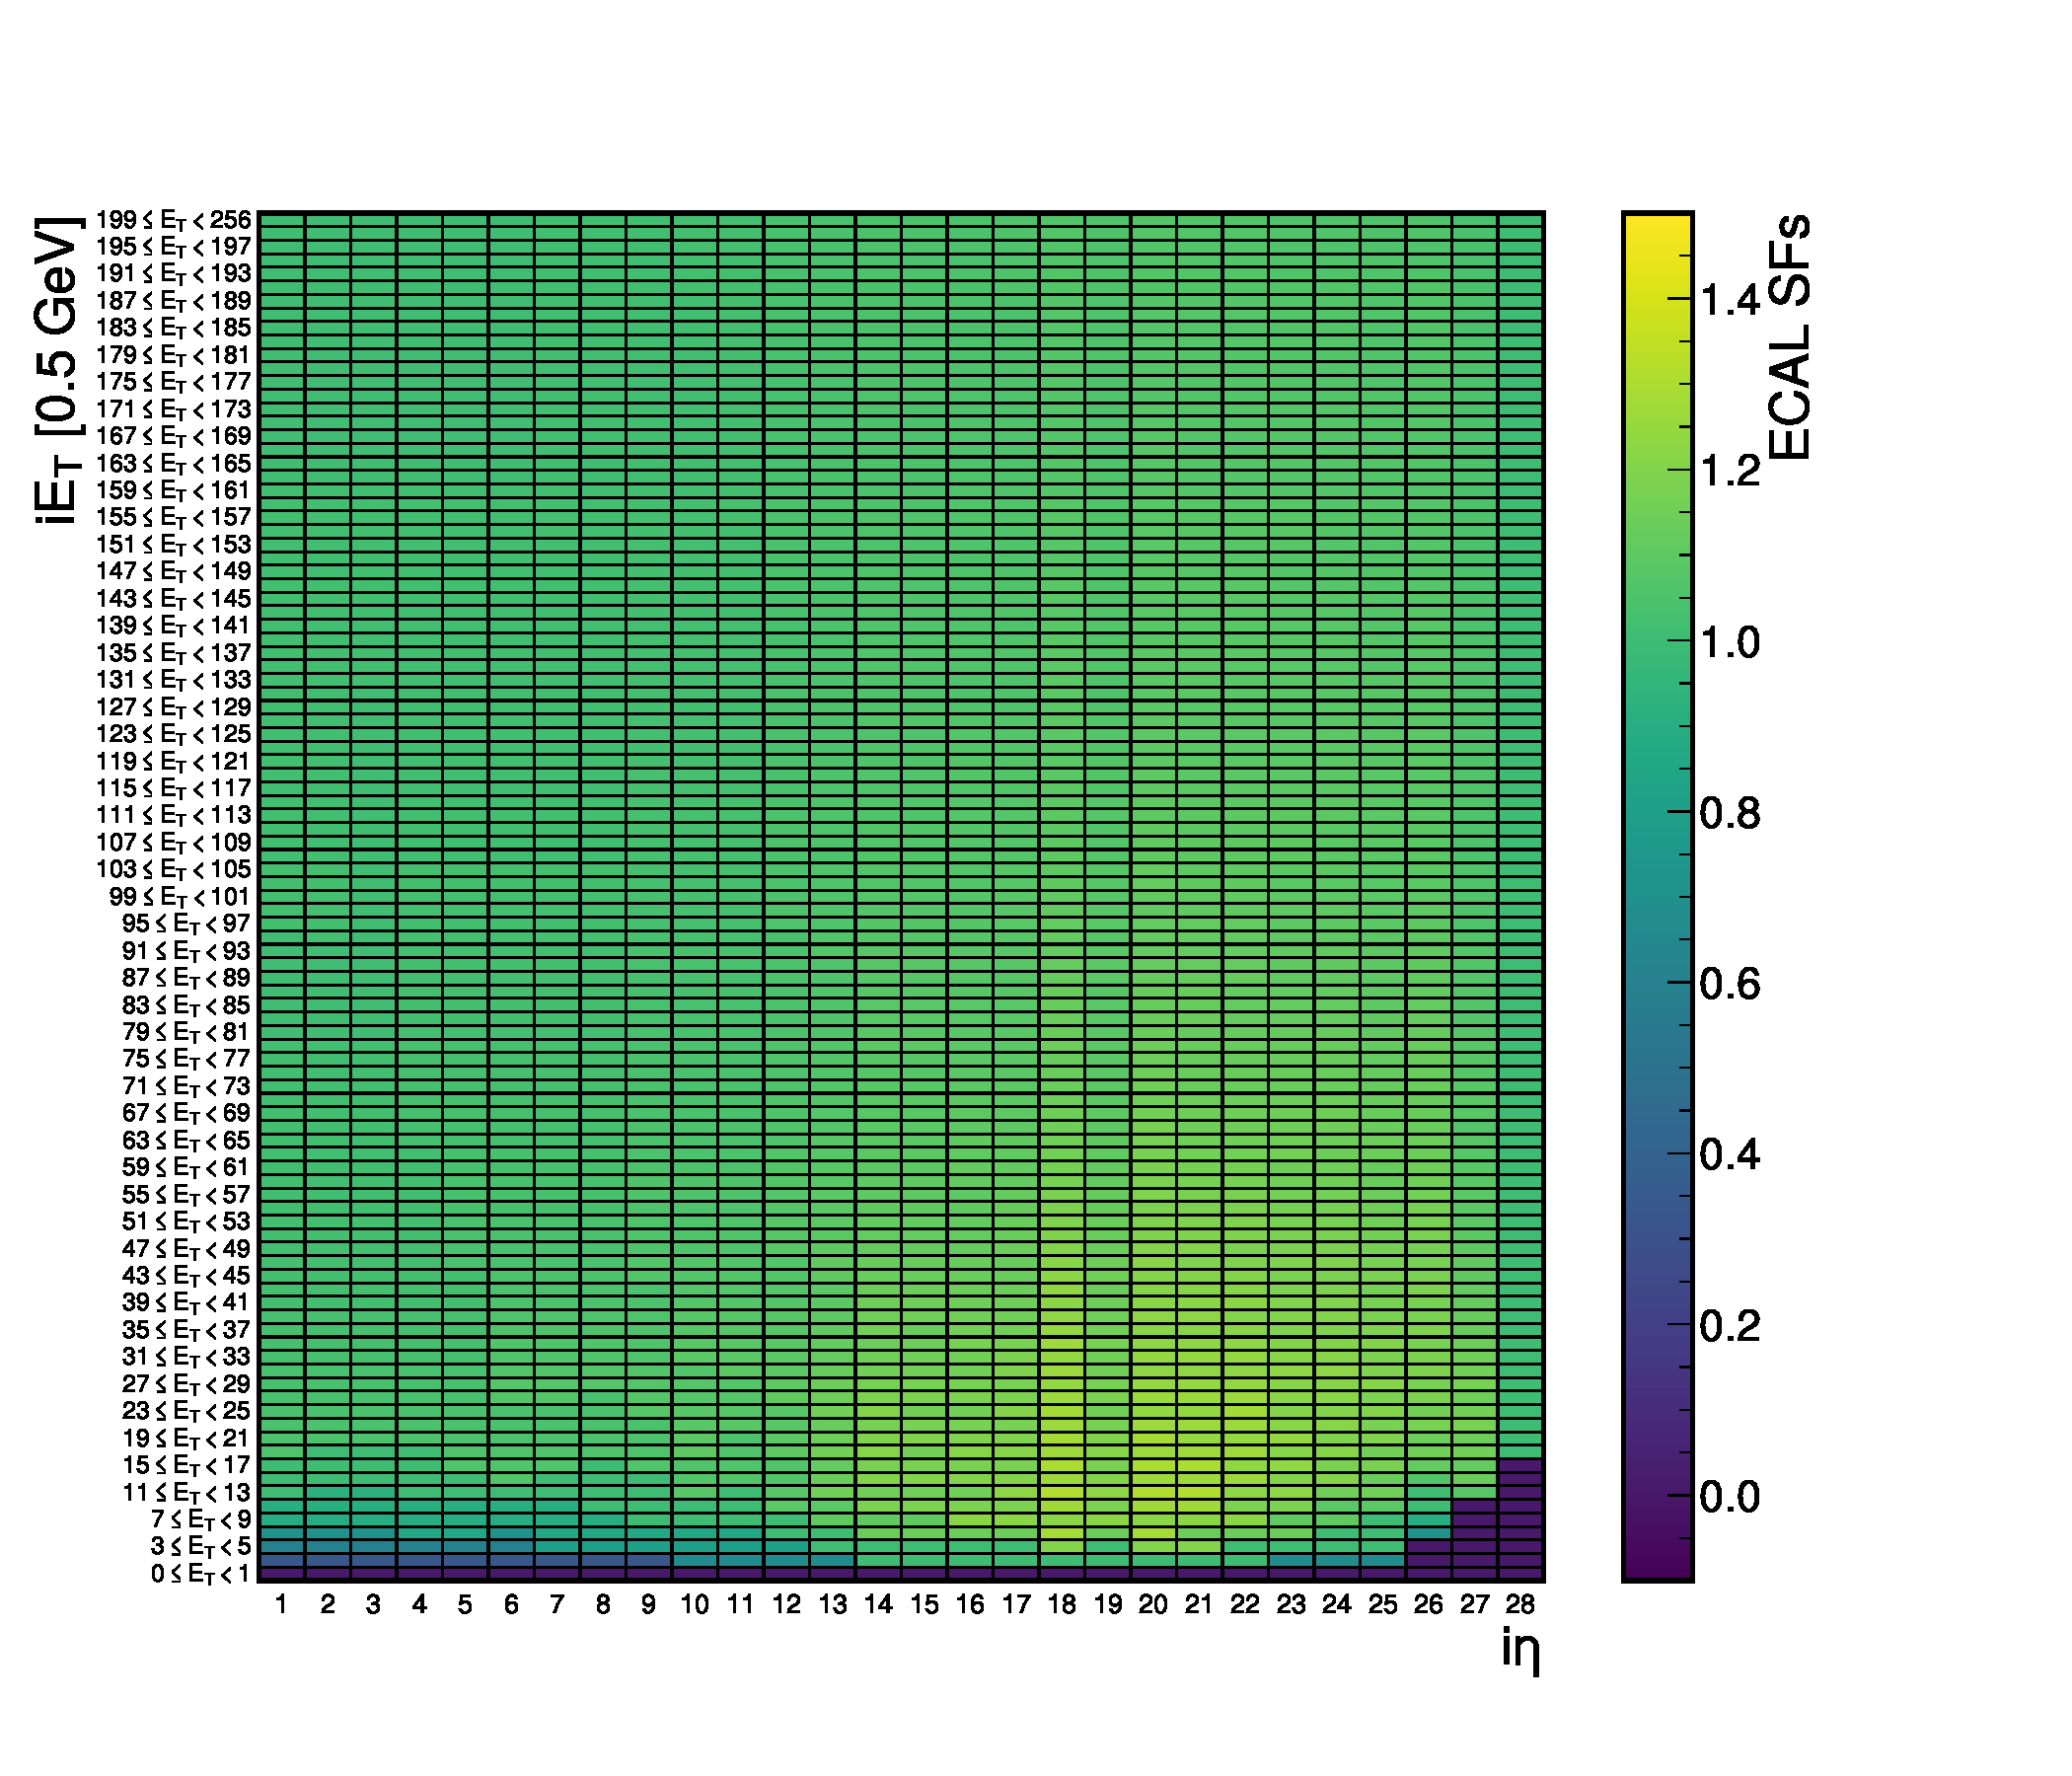
\includegraphics[width=0.5\linewidth]{Figures/L1TP/SFs_2D_ECAL_Thesis_NN.pdf}}
    \caption{Layer-1 ECAL calibration factors derived from the current method (a), and extracted through the NN approach (b). The colour map represents the calibration factor value, lower (higher) for darker (brighter) shades. Each bin corresponds to a give $i\eta$ position and range of raw energy deposit, in $iE_T$ units, corresponding to 0.5~GeV. With the new NN-based method for the Layer-1 calibration, the scale factors granularity is significantly increased, while maintaining the expected patterns corresponding to transition from barrel to endcap ($i\eta=18$), where the depth of the ECAL crystals is reduced and the energy deposit is compensated by higher calibration factors.}
    \label{fig:ECALSFs_NN}
\end{figure}

\begin{figure}
    \centering
    \subfloat[Current method (HCAL)]{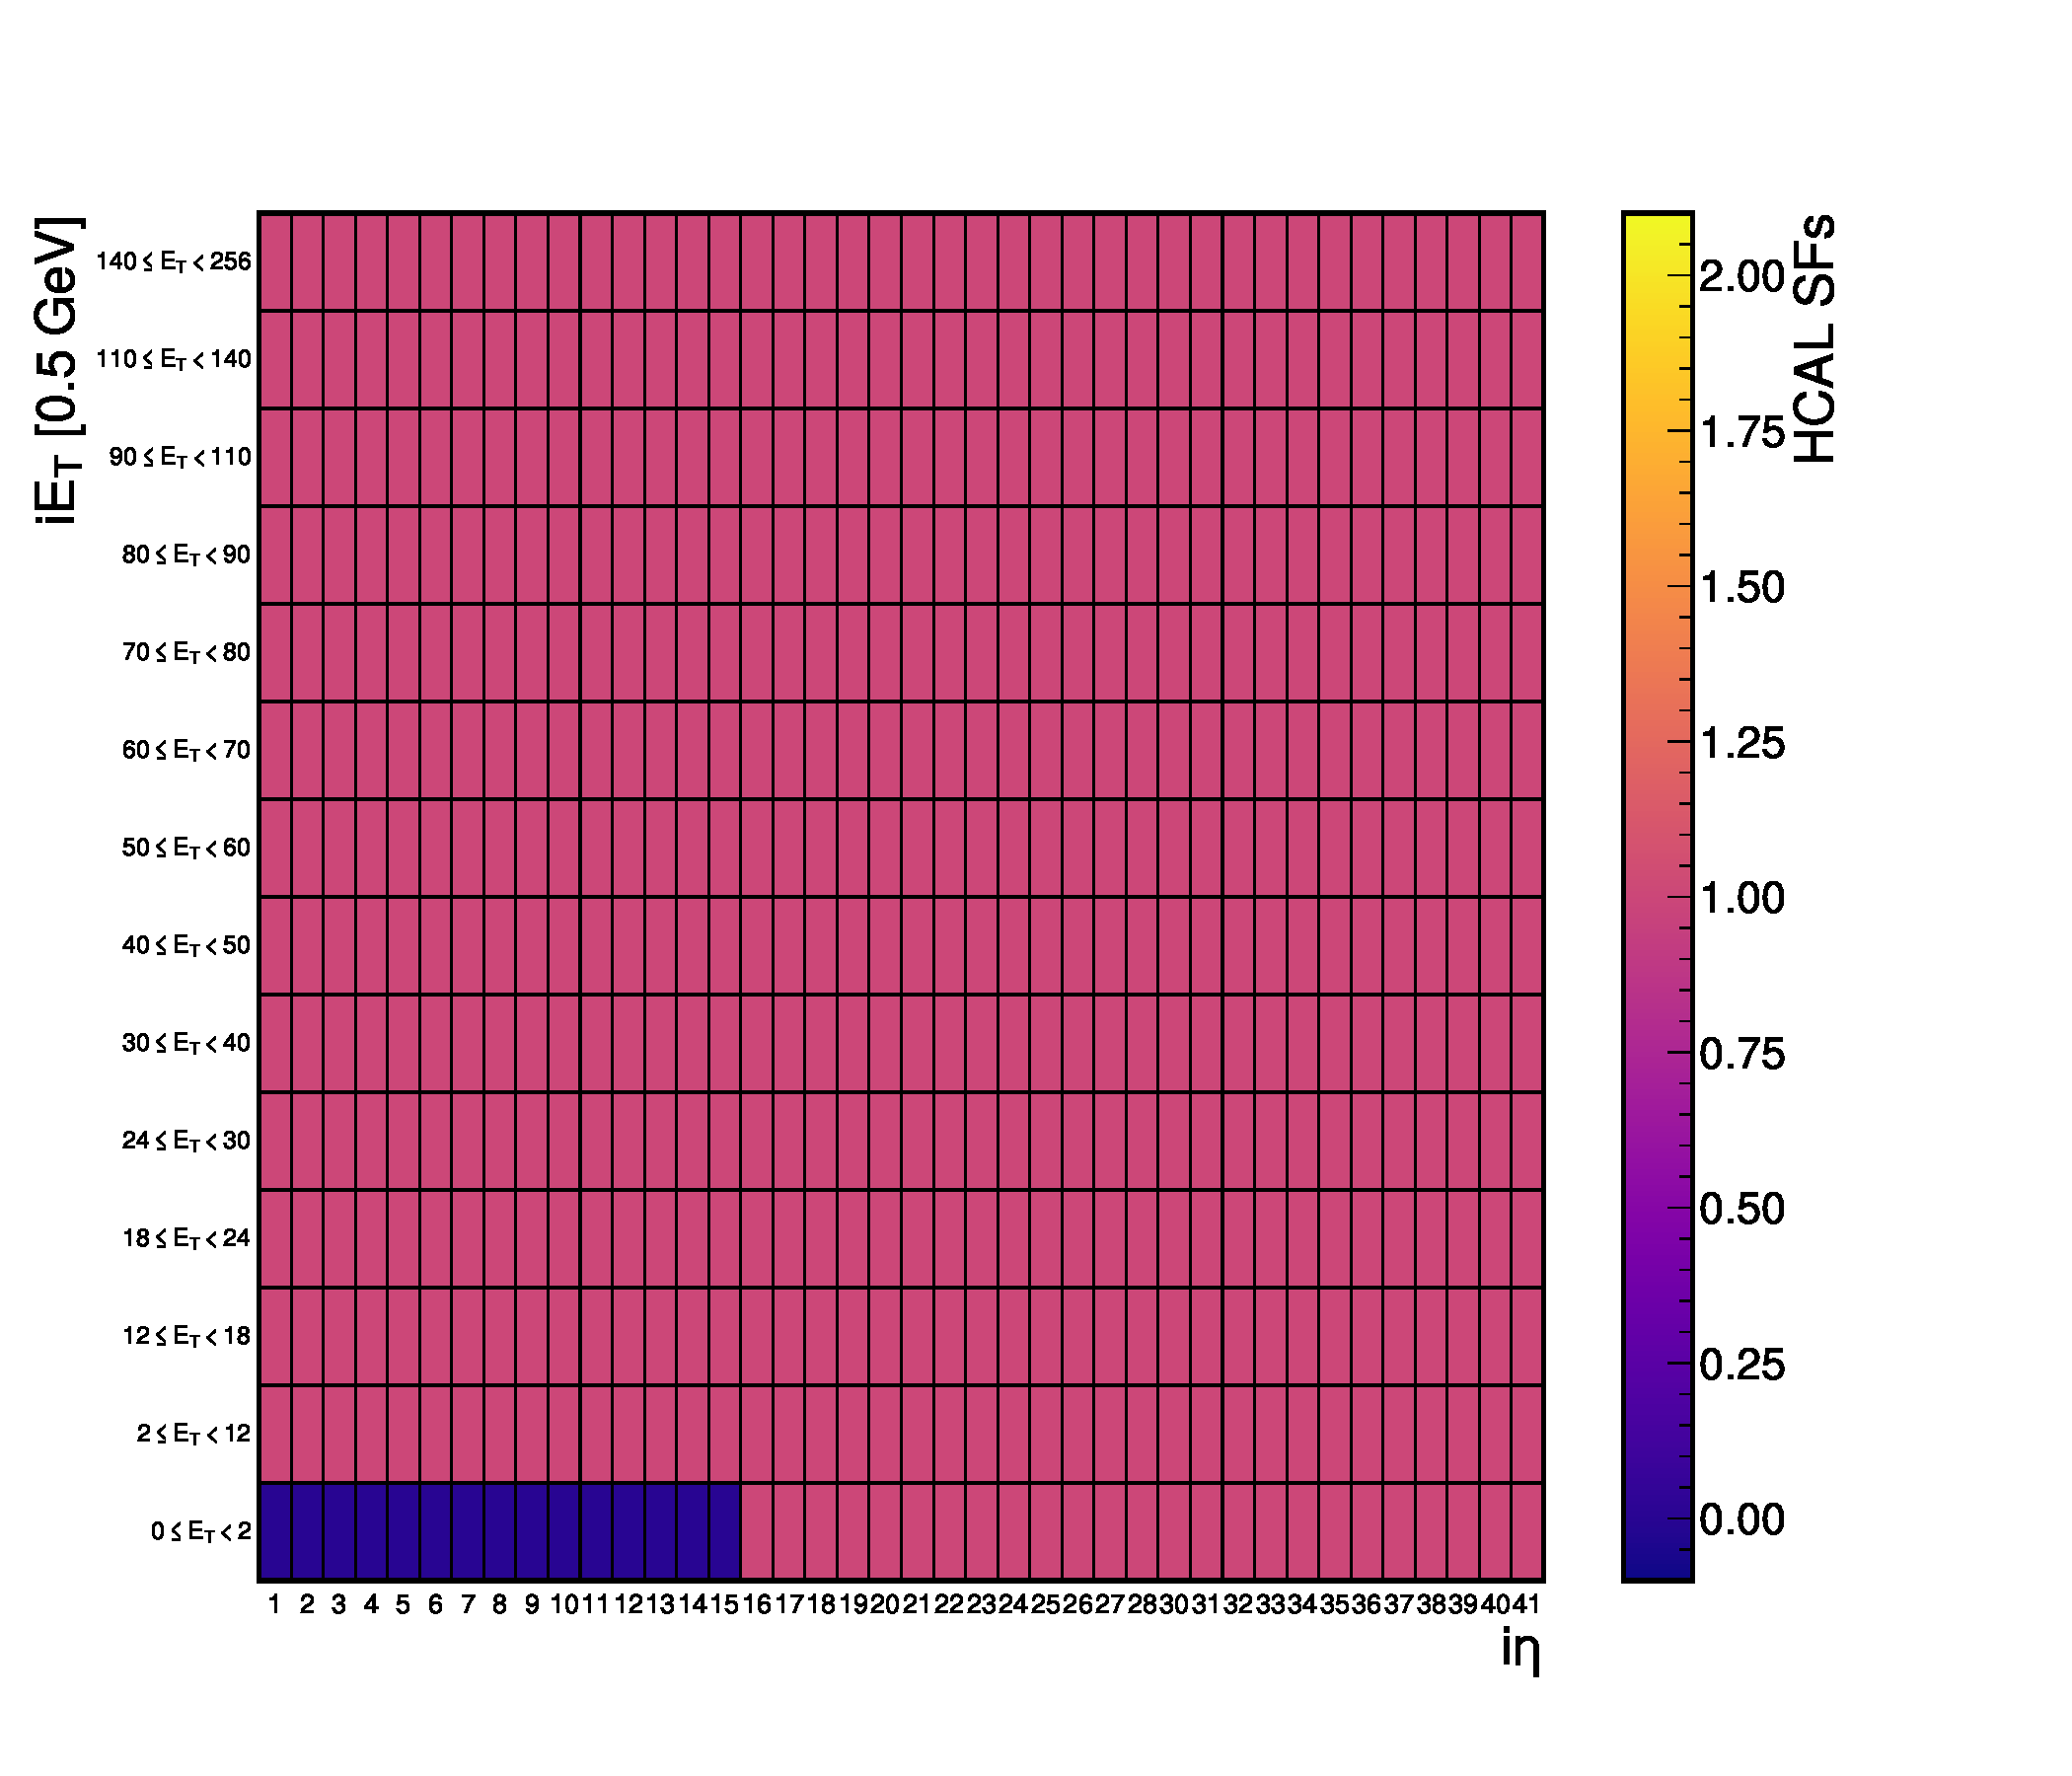
\includegraphics[width=0.5\linewidth]{Figures/L1TP/SFs_2D_HCAL_Thesis.pdf}}
    \subfloat[NN method (HCAL)]{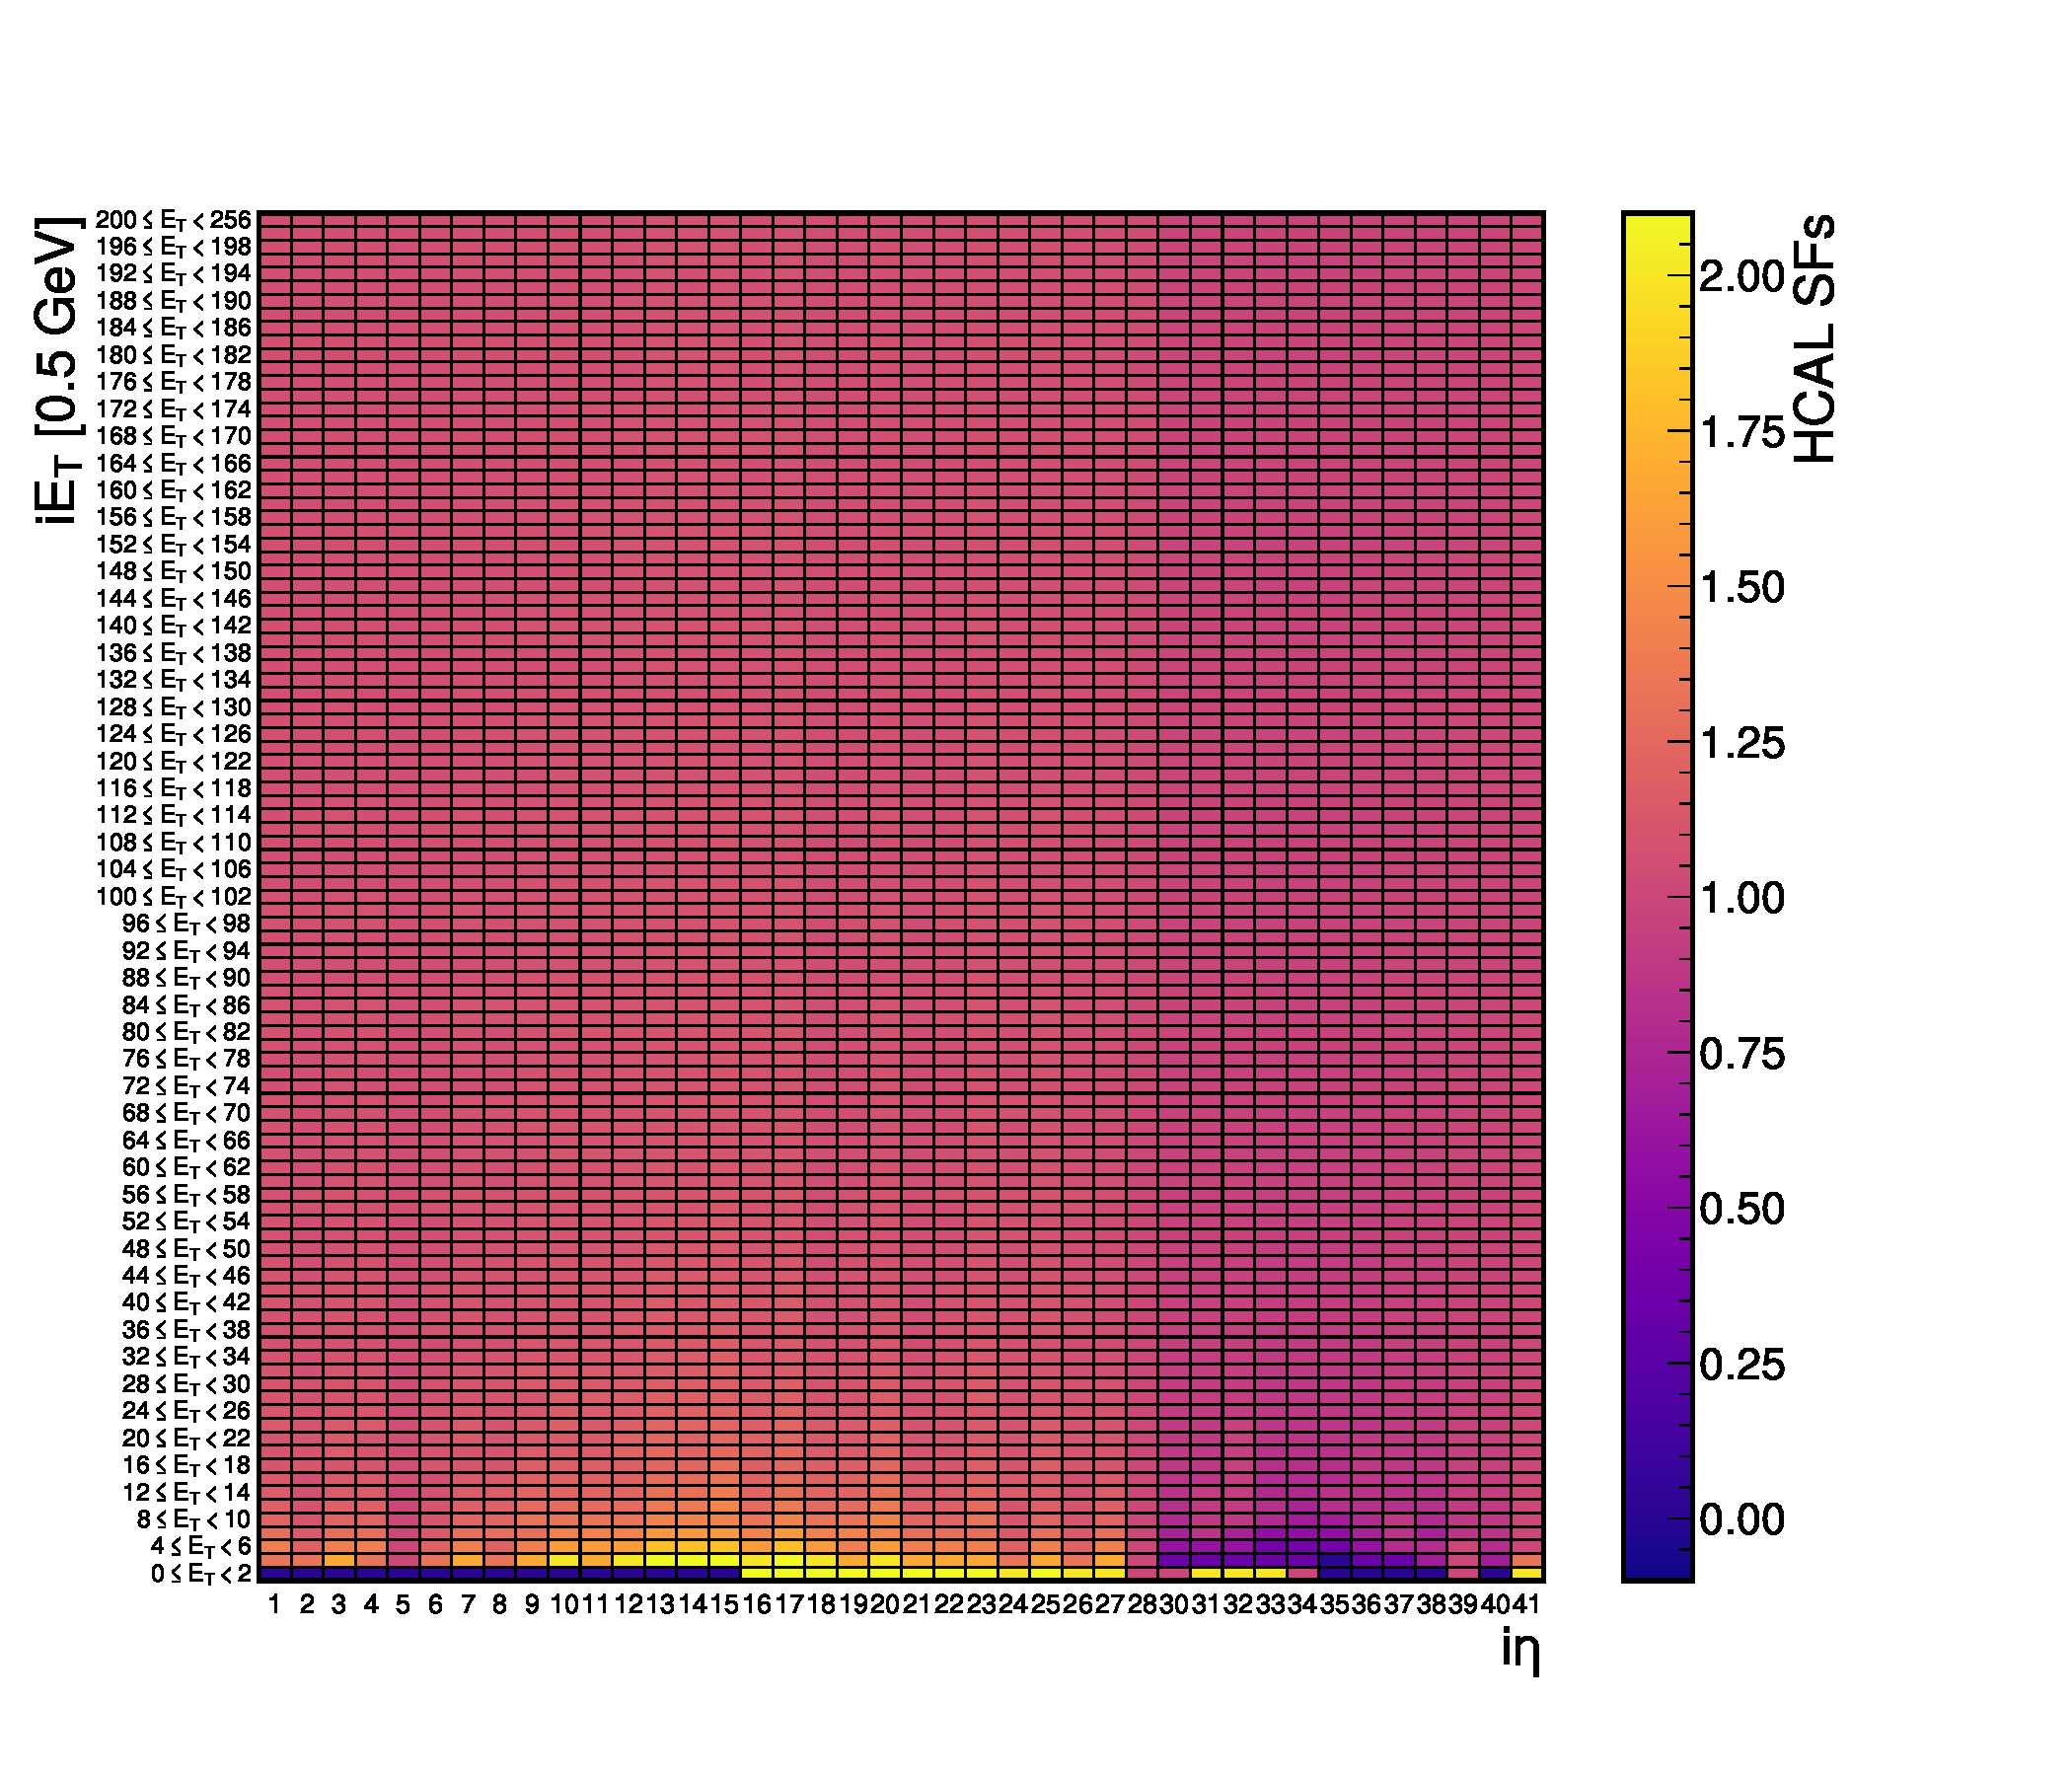
\includegraphics[width=0.5\linewidth]{Figures/L1TP/SFs_2D_HCAL_Thesis_NN.pdf}}
    \caption{Layer-1 HCAL calibration factors currently online (a), and extracted through the NN approach (b). The colour map represents the calibration factor value, lower (higher) for darker (brighter) shades. Each bin corresponds to a give $i\eta$ position and range of raw energy deposit, in $iE_T$ units, corresponding to 0.5~GeV. The current Layer-1 configuration for HCAL only includes zero-suppression in the barrel for $E_T=0.5$~GeV and $|i\eta|\leq 15$.
    % ; a zero-suppression is only applied to TTs recording $E_T=0.5$~GeV in the region $|i\eta|\leq 15$, to reduce the pile-up contribution in the barrel. 
    The new NN-based method for the Layer-1 calibration enhances the recorded energy in the region around $i\eta=17$, corresponding to the transition between HCAL barrel and endcap.}
    \label{fig:HCALSFs_NN}
\end{figure}

The calibration factors extracted by the NN approach, and compared to the current approach, are reported in Figure~\ref{fig:ECALSFs_NN}-\ref{fig:HCALSFs_NN} for the ECAL and HCAL TTs respectively, as a function of the $i\eta$ position and the energy.
The new NN-based approach is capable of providing a much higher granularity in the energy dimension, extracting through a single training process a total of 2,800 calibration factors for ECAL, and 4,100 for HCAL and HF: the calibration factors are derived in energy bins of 2~$iE_T$, up to a maximum value of $iE_T=100$~GeV, after which one single energy bin is considered. 

In the case of ECAL, the calibration factors are close to unity, with a slight suppression of TTs in the barrel recording low energy deposit, and a visible enhancement of TTs in the endcap. A discontinuity is noticeable for the region corresponding to $i\eta=18$, already present in the previous configuration of calibration factors: this region marks the transition from barrel to endcap, as shown in Figure~\ref{fig:Layer1}, where the depth of the ECAL crystals is reduced and a smaller energy deposit needs to be compensated by higher calibration factors. The six suppressed low energy towers corresponding to $i\eta=26,27,28$ are manually constrained to 0 in the extracted LUT, following Layer-1 recommendations, to reduce the impact of the most forward ECAL TTs, significantly affected by radiation damage.

In the case of HCAL, the calibration factors generally show larger values, especially for low energy TTs and in the region around $i\eta=17$, where the depth of HCAL crystals is reduced by the geometry of the detector. In the HF compartment, the newly derived calibration factors present a change with respect to the previous configuration, showing a tendency to suppress the TTs raw energy, by applying factors below unity. While the previous method was based on MC samples produced in the ideal environment of no pile-up, the NN is trained on real data, where the pile-up effect, which is predominant in the HF region, contaminates the L1 candidate: the NN learns how to suppress the additional energy contribution coming from pile-up and results in lower calibration factors across the HF region.

\bigbreak

% performance
The performance of the newly derived Layer-1 calibration factors can be evaluated by replicating the Layer-1 firmware implemented in the hardware of the CMS service cavern with the new LUTs. A dataset collected by the CMS experiment during Run~III data taking is re-emulated under three different Layer-1 configurations: one in which no calibration is applied (\textit{No calibration}), one in which the calibration factors are set to the values obtained with the old method (\textit{Old calibration}), and one in which the calibration constants are derived with the NN approach presented in this section (\textit{New calibration}).
The three configurations are compared in terms of Layer-1 energy response, defined as the ratio between the L1 $e/\gamma$ or jet candidate energy and the offline reconstructed electron of PUPPI jet energy. From the differential distribution of the Layer-1 energy response, the mean of the distribution defines the energy scale, which is expected to be as close as possible to unity, while the ratio between the standard deviation and the mean defines the energy resolution, which needs to be minimised for a performance improvement.
However, the resolution is only a partial aspect of the Layer-1 trigger performance, which has to be evaluated in terms of expected rate and efficiency. A commonly used figure of merit for the L1 performance evaluation is the efficiency turn-on curve, which describes, for a given L1-$p_T$ threshold, the efficiency in detecting and reconstructing the L1 candidates that are correctly matched to offline candidates with the same energy. The efficiency turn-on curve is computed as the ratio between offline-$p_T$ distribution of the objects matched to a L1 candidate passing the L1-$p_T$ threshold and the offline-$p_T$ distribution of all offline objects. 
Ideally, the efficiency turn-on curve should be centered around the L1-$p_T$ threshold, with minimum efficiency for objects below the thresholds and maximum efficiency above the threshold. 
In reality, the definition of the L1 energy is not always accurate, given the reduced information available, and can be either under-estimated or over-estimated, leading potential inefficiencies or false positives and resulting in a less steep turn-on curve.
To account for differences in the rate and ensure a fair comparison of the different methods, the efficiency turn-on curves computed for L1-$p_T$ thresholds providing the same Layer-1 rate are compared to each other.

\bigbreak

\begin{figure}
    \centering
    \subfloat[Inclusive Response]{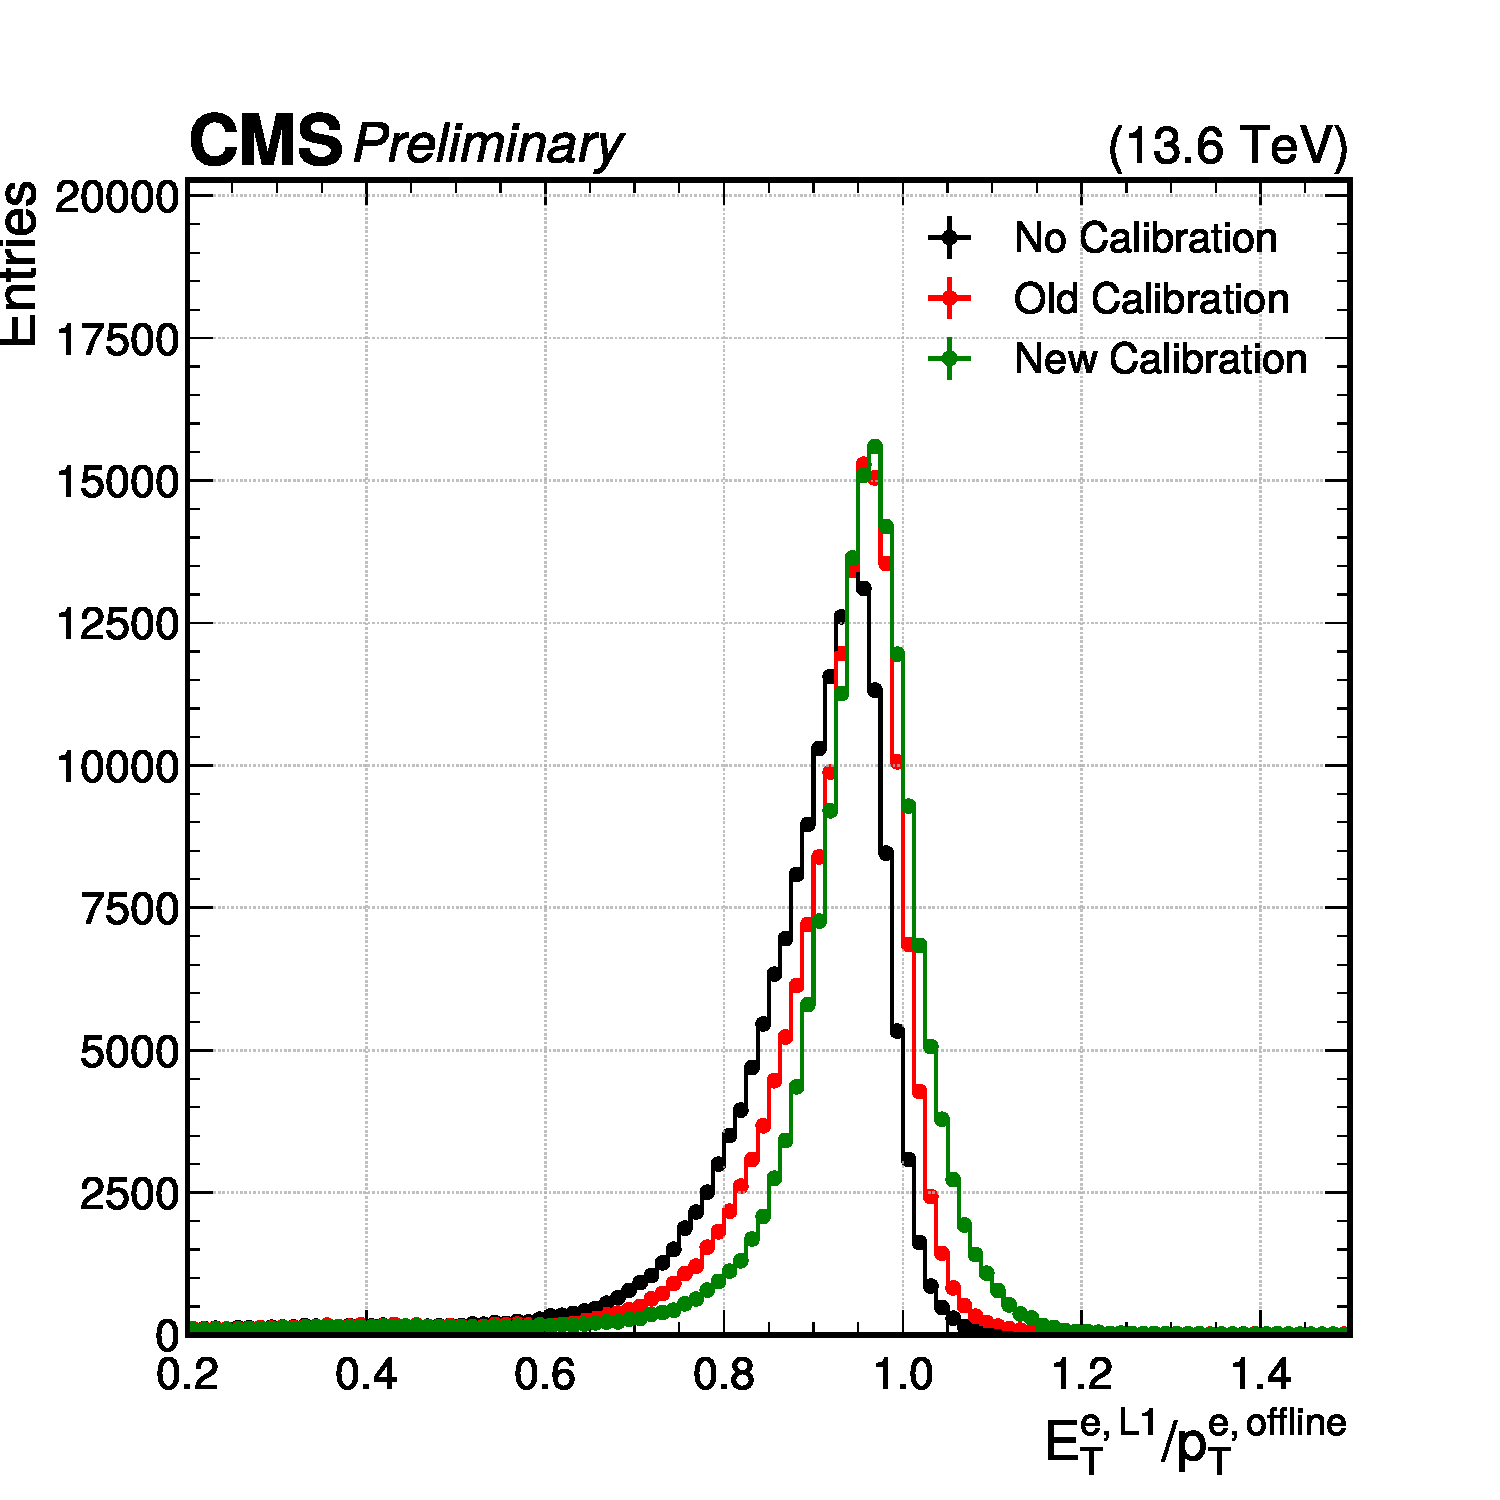
\includegraphics[width=0.5\linewidth]{Figures/L1TP/NN_Performance/response_inclusive__ele.pdf}}
    
    \subfloat[Energy Resolution]{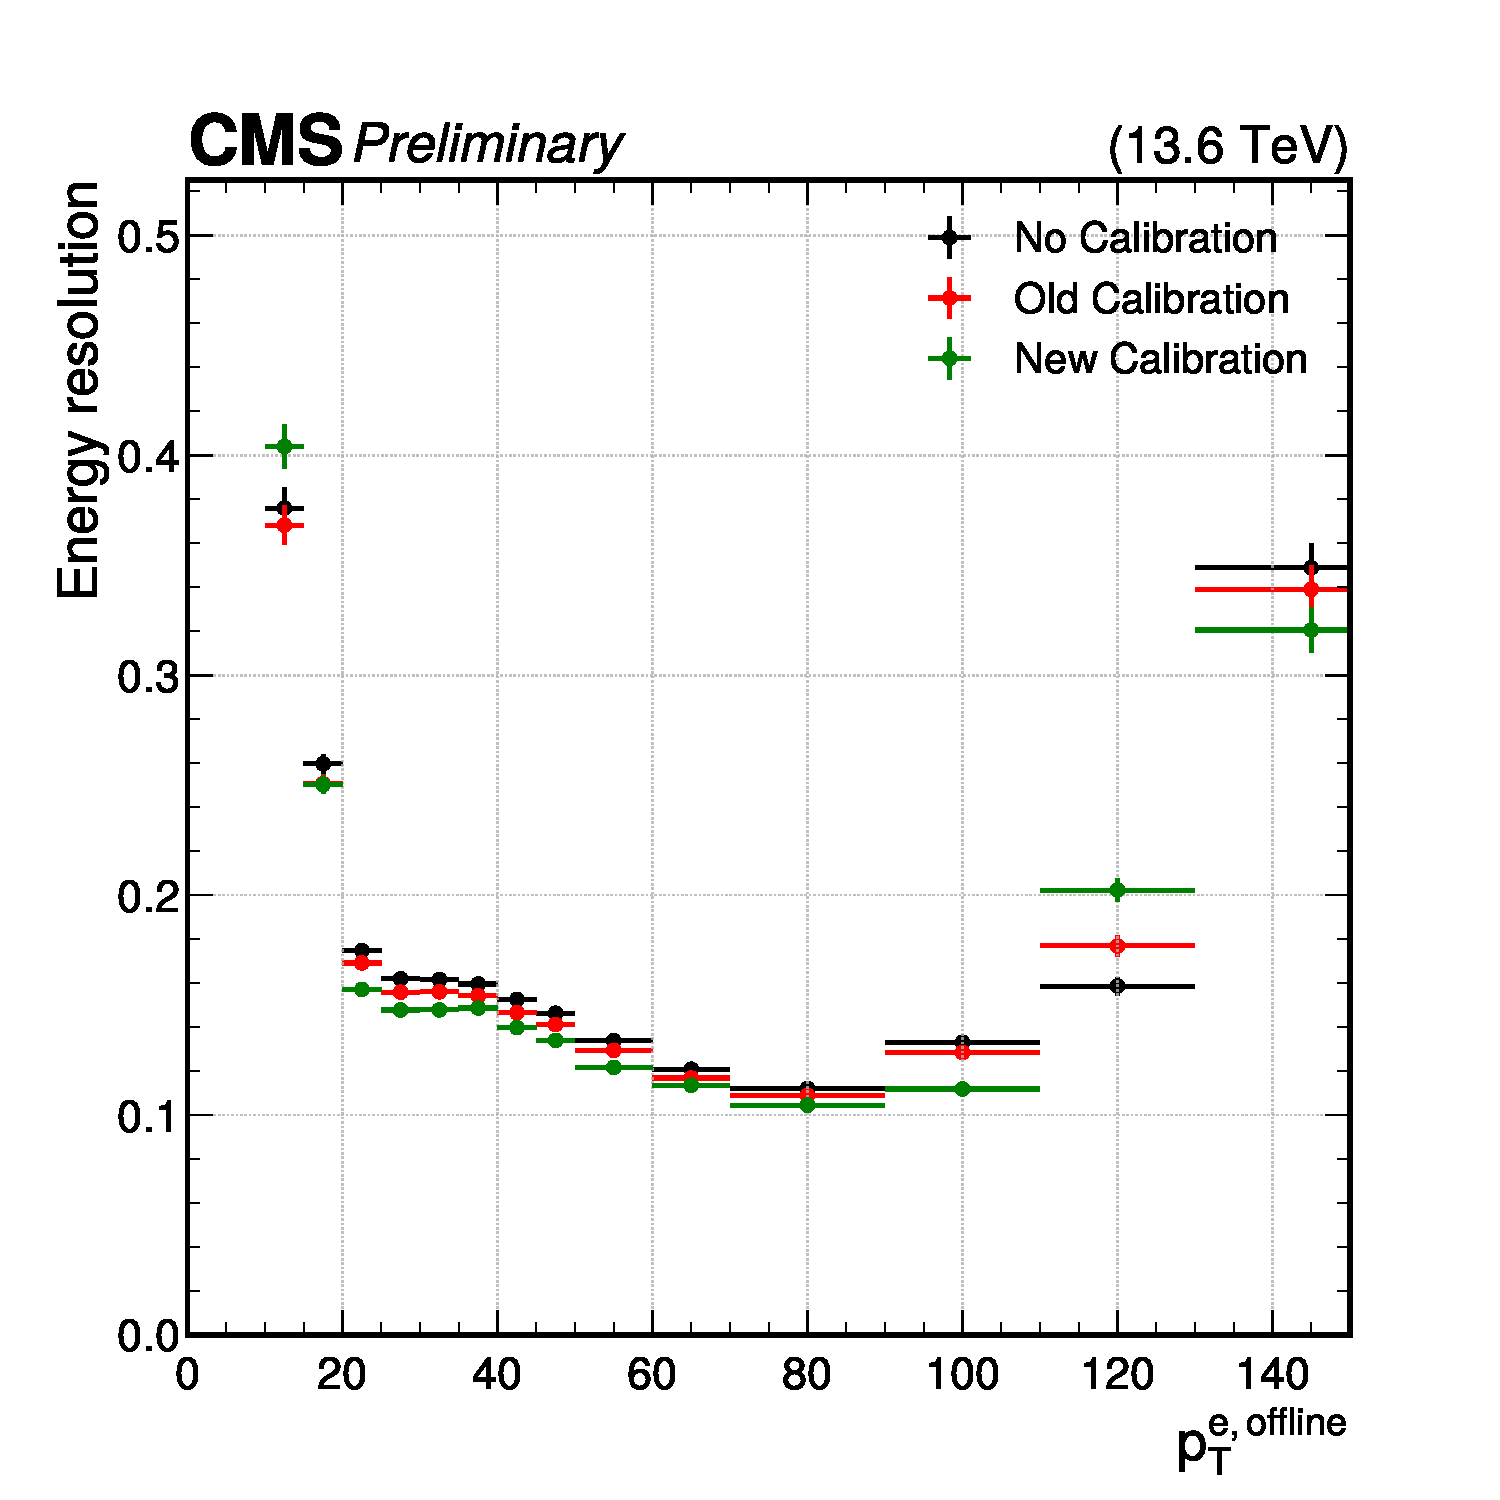
\includegraphics[width=0.5\linewidth]{Figures/L1TP/NN_Performance/resolution_ptBins__ele.pdf}}
    \subfloat[Energy Scale]{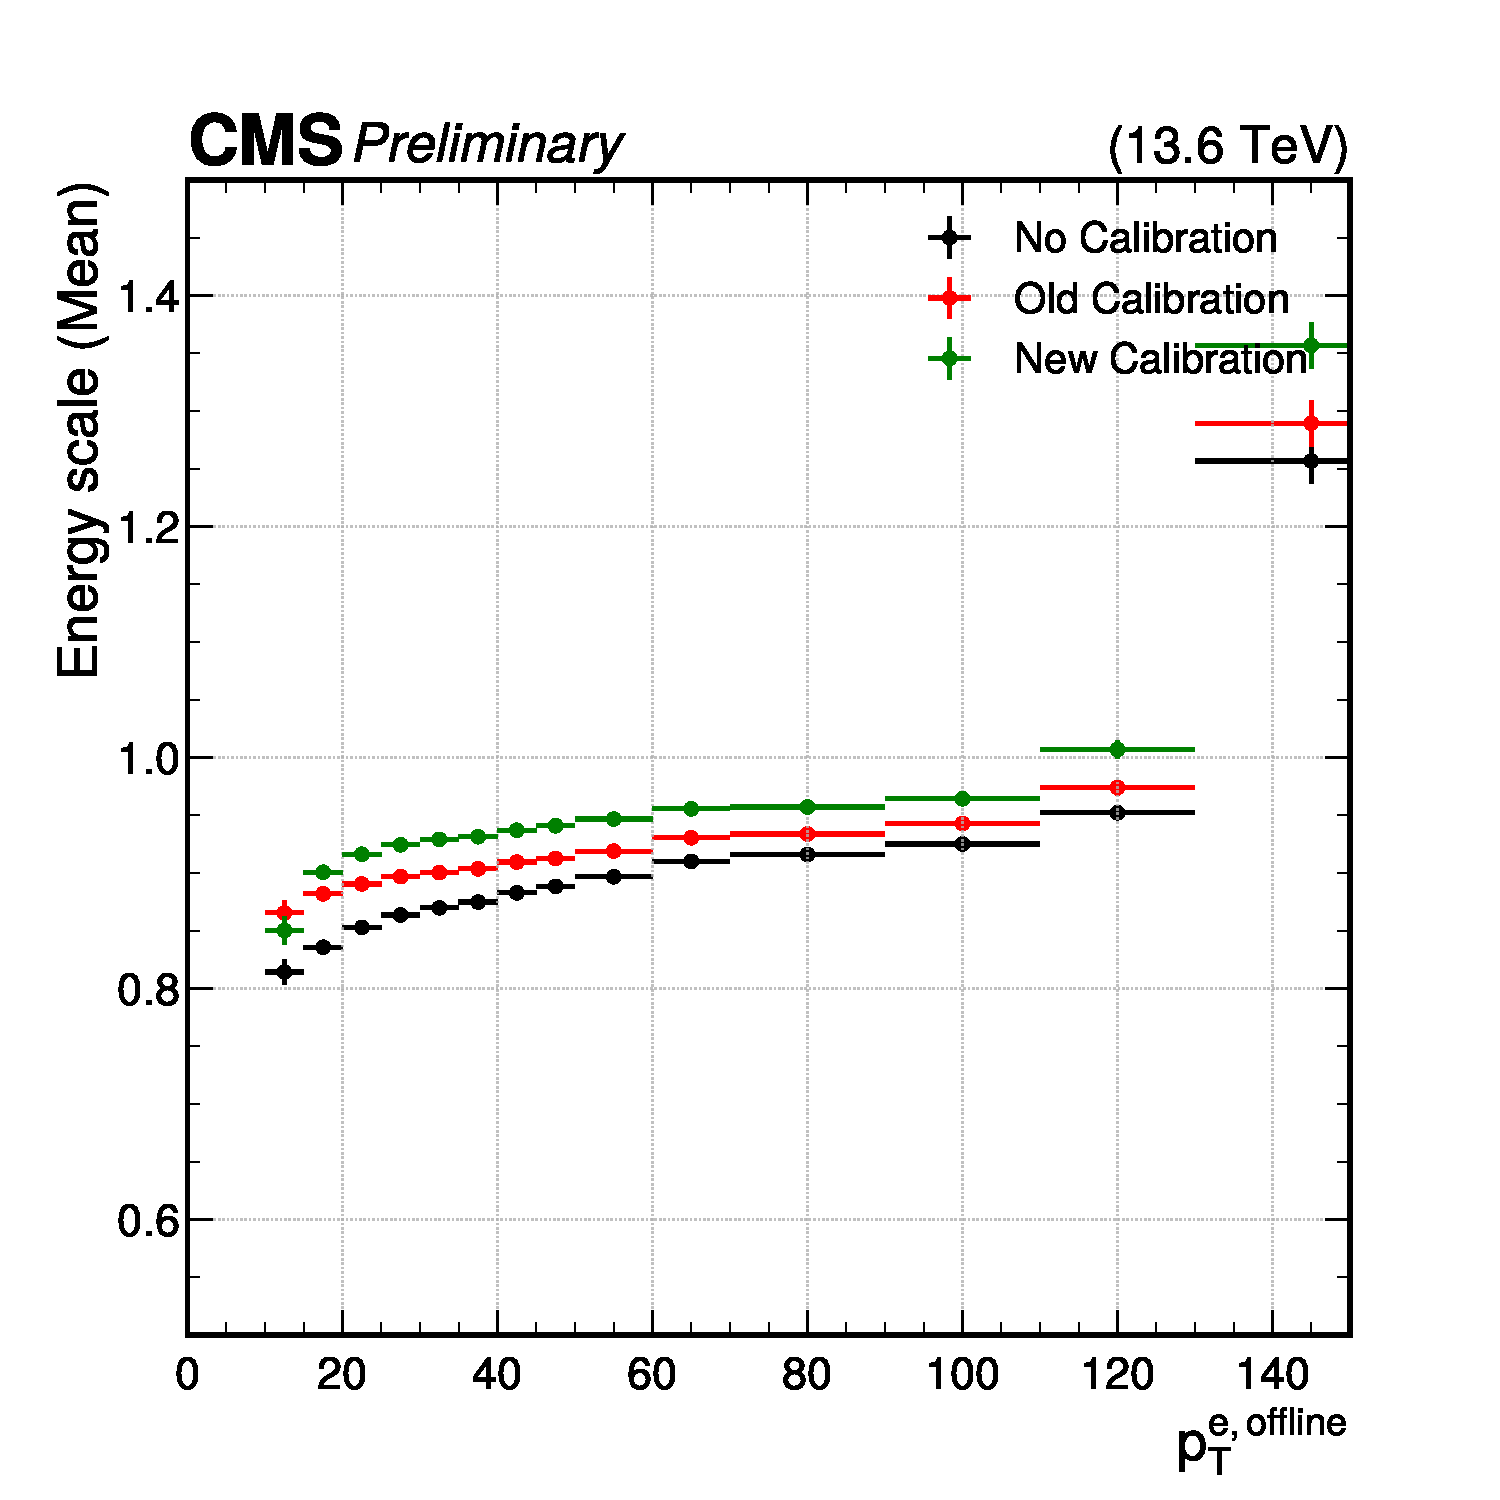
\includegraphics[width=0.5\linewidth]{Figures/L1TP/NN_Performance/scale_ptBins__ele.pdf}}
    \caption{Layer-1 $e/\gamma$ performance of the calibration factors derived through the NN approach, in terms of energy response (a), energy resolution (b) and energy scale (c) as a function of the offline $p_T$. The energy of the L1 $e/\gamma$ candidate is obtained by replicating the Layer-1 firmware with three different configurations: no calibration (black), old calibration (red), and new NN-based calibration (green); no Layer-2 calibration is applied to the L1 candidate.}
    \label{fig:NN_ECAL_Response}
\end{figure}

\begin{figure}
    \centering
    \subfloat[Rate]{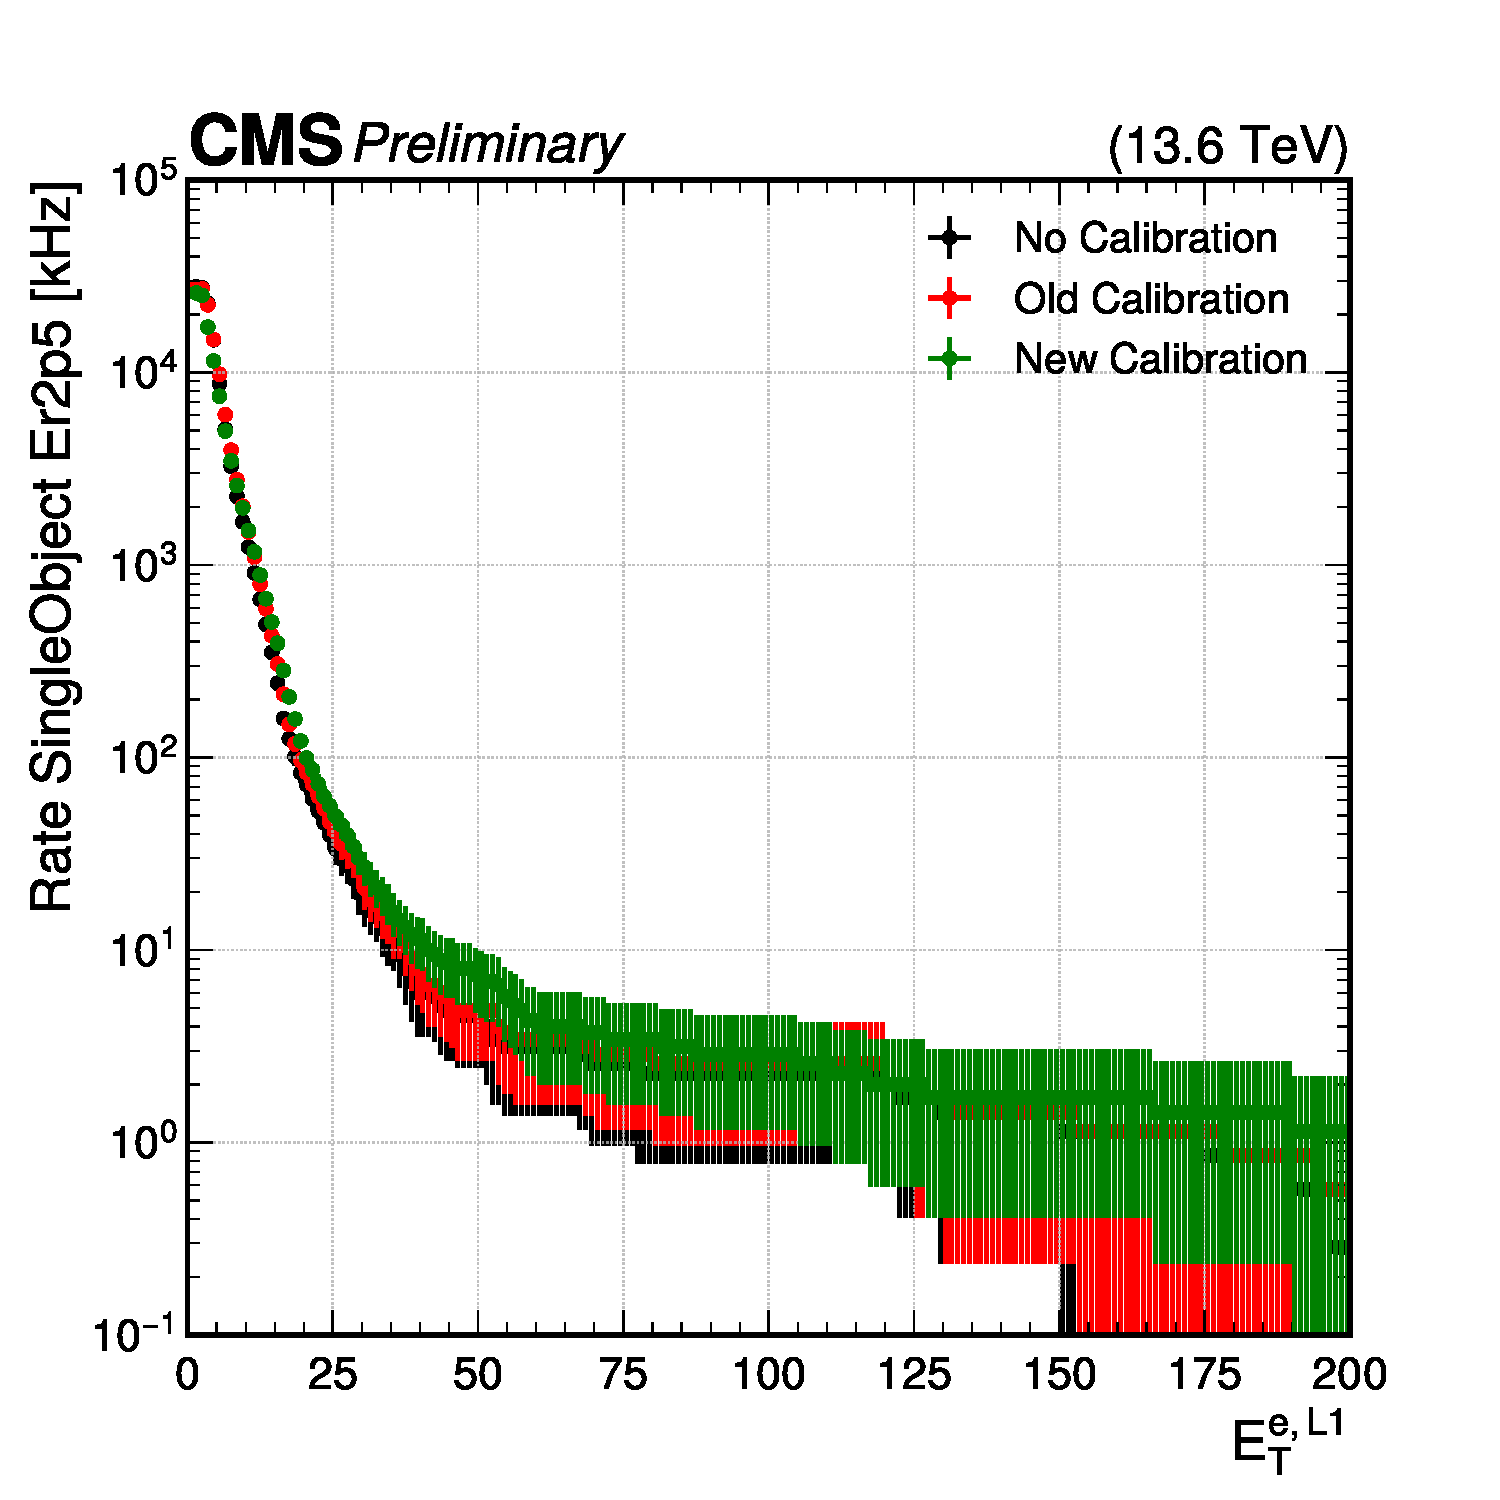
\includegraphics[width=0.5\linewidth]{Figures/L1TP/NN_Performance/rate_ObjEr2p5__ele.pdf}}
    
    \subfloat[Efficiency turn-on: $p_T>12$~GeV]{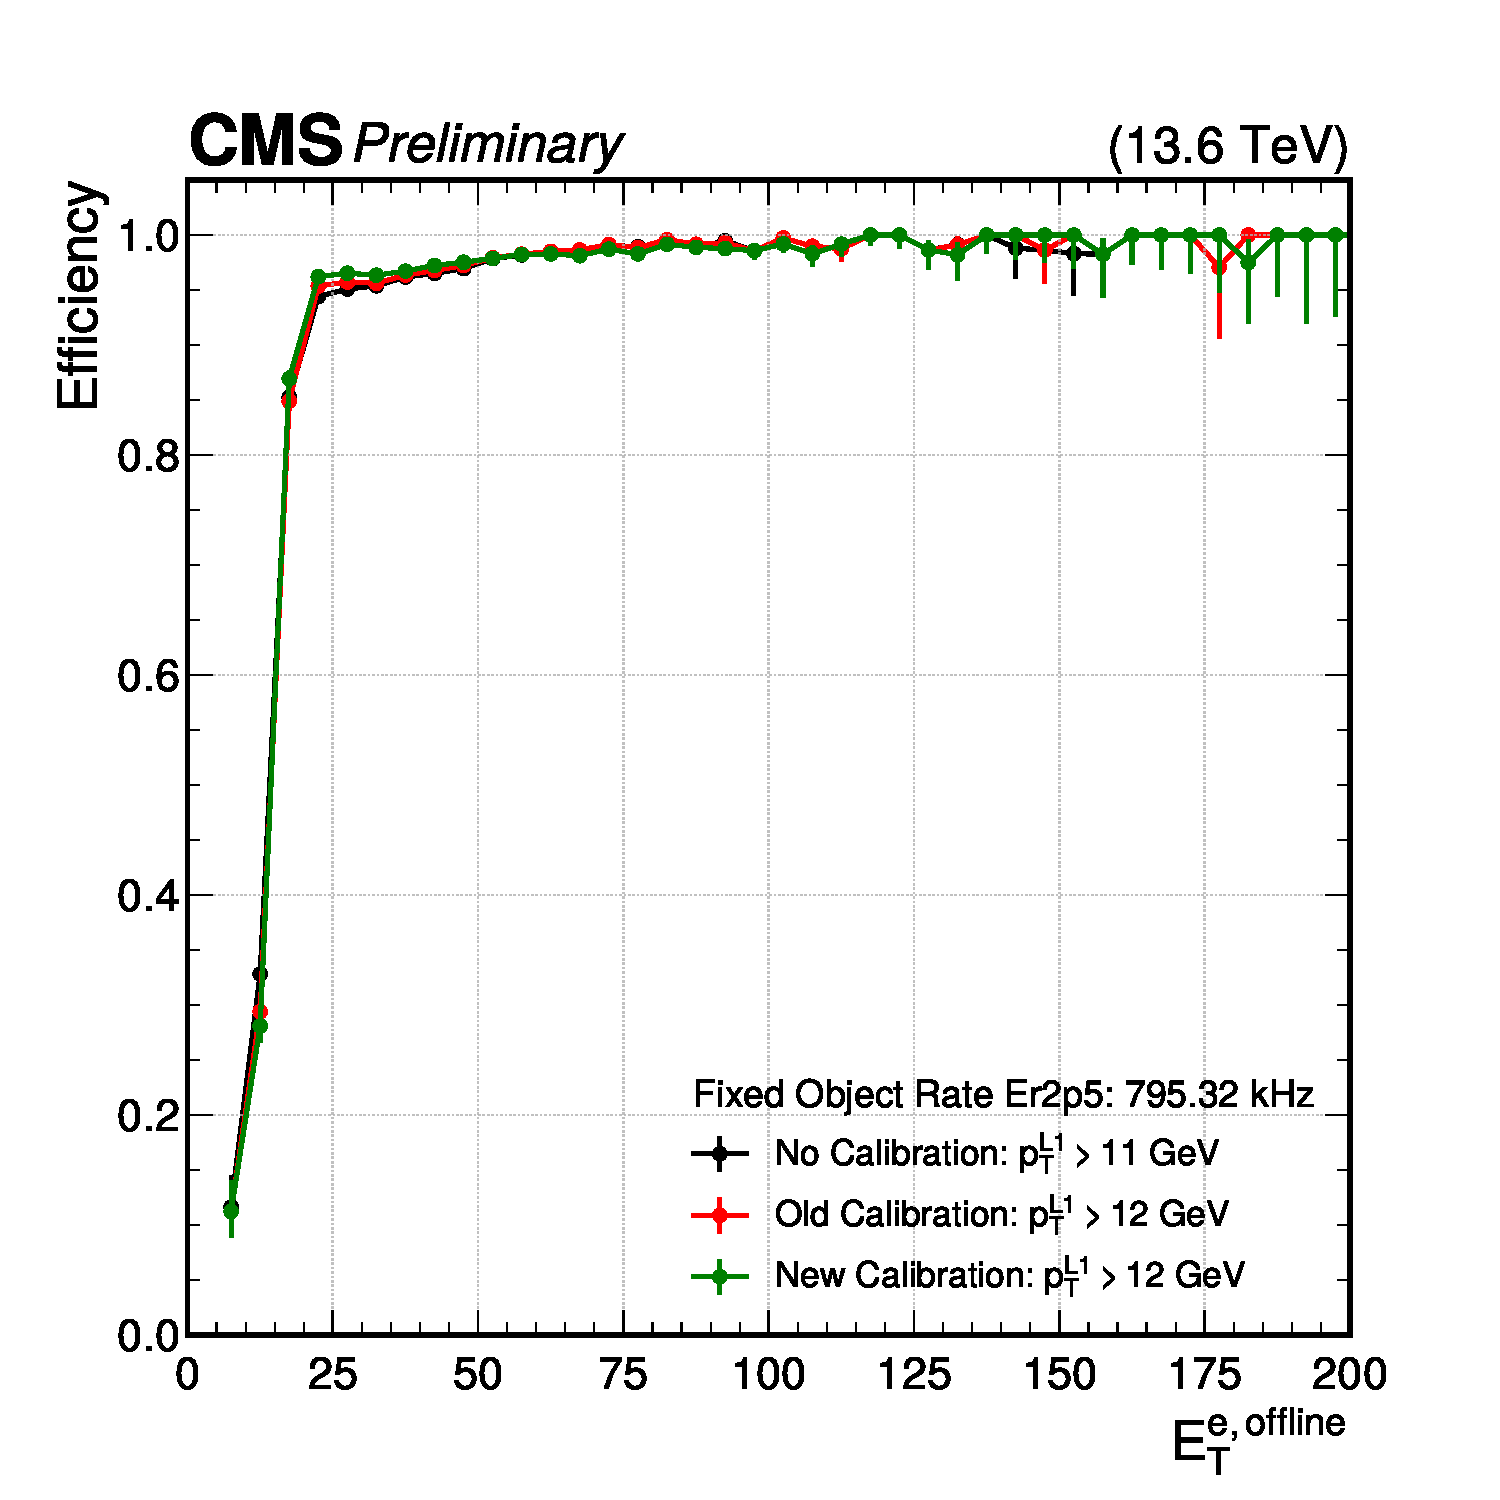
\includegraphics[width=0.5\linewidth]{Figures/L1TP/NN_Performance/turnon_fixedObjRateEr2p5_12__ele.pdf}}
    \subfloat[Efficiency turn-on: $p_T>20$~GeV]{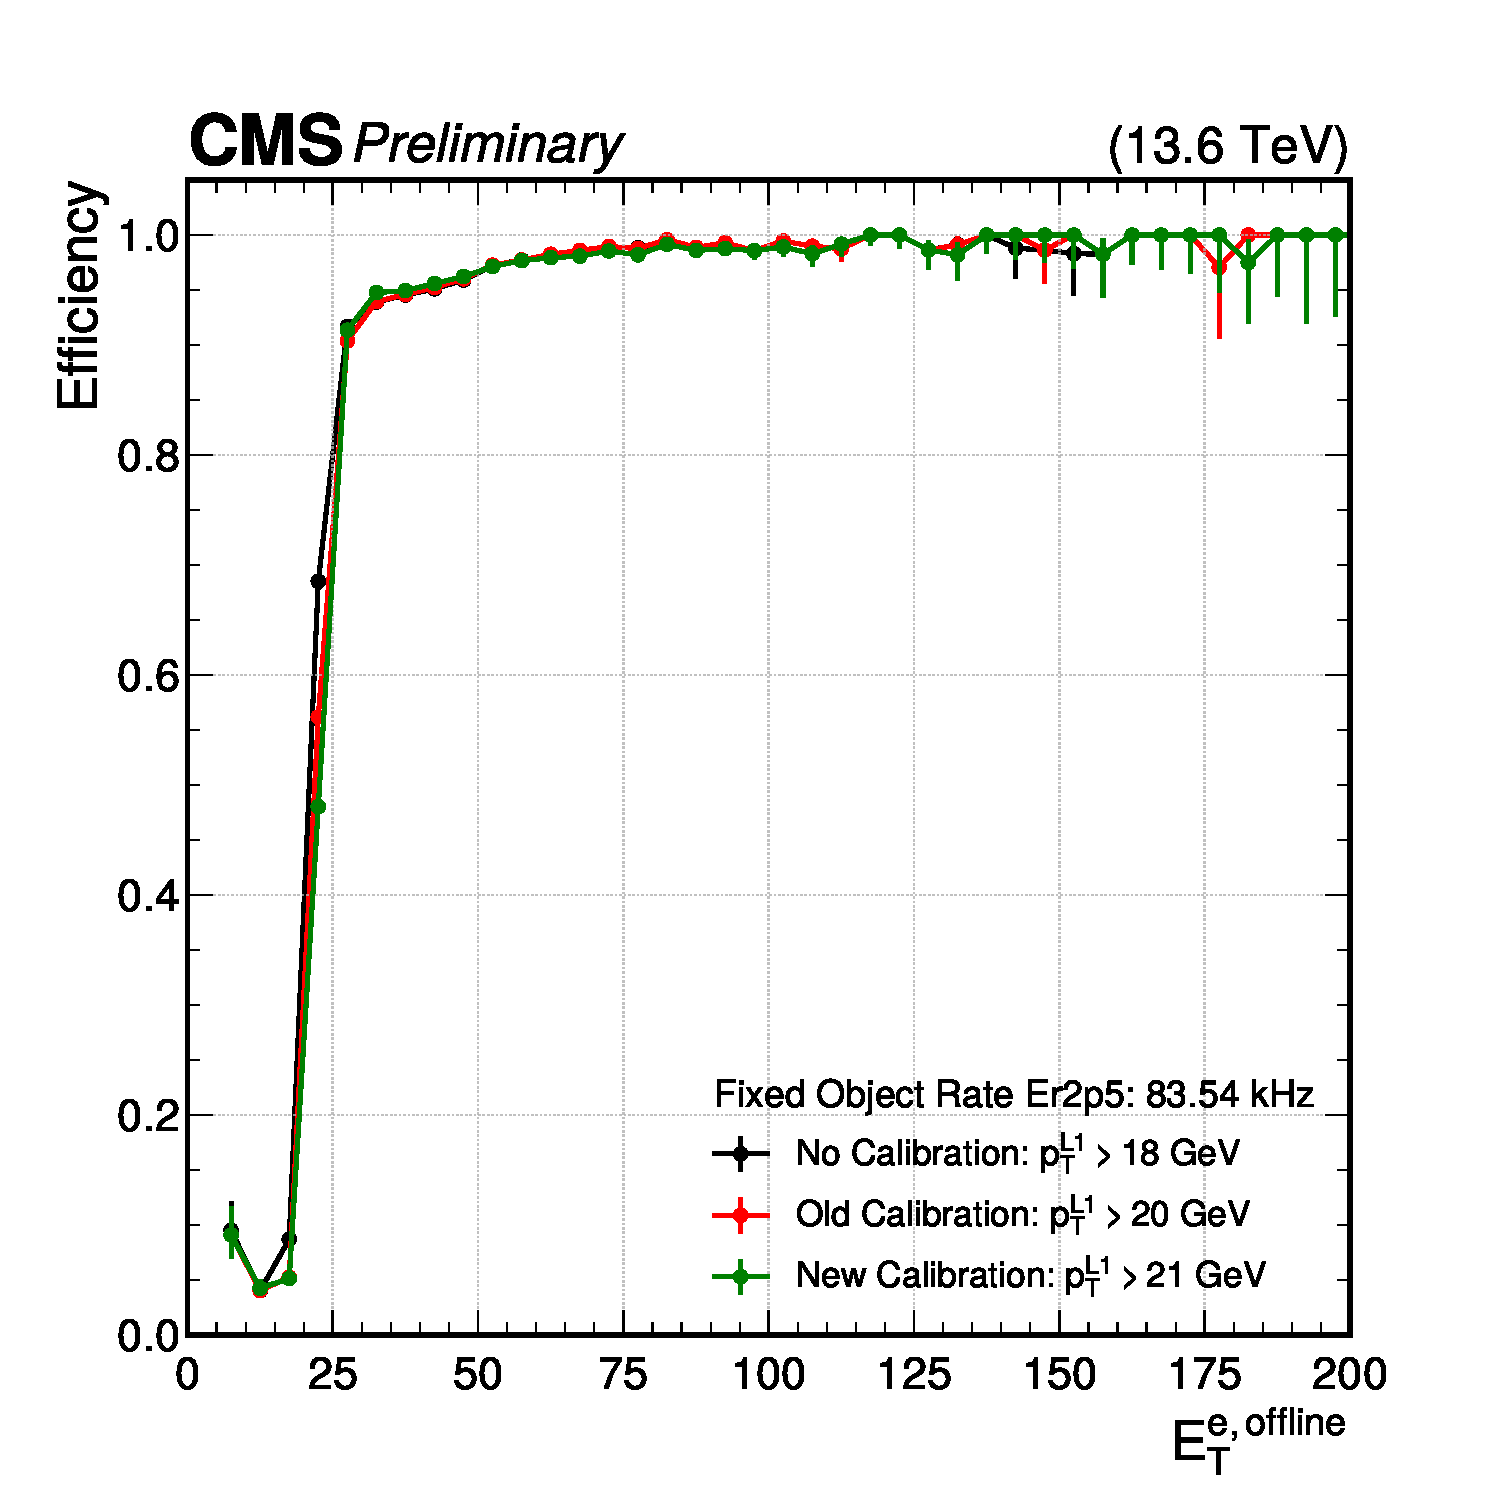
\includegraphics[width=0.5\linewidth]{Figures/L1TP/NN_Performance/turnon_fixedObjRateEr2p5_20__ele.pdf}}
    \caption{Layer-1 $e/\gamma$ performance of the calibration factors derived through the NN approach, in terms of rate (a) and efficiency turn-on curves (b-c) for two fixed rate thresholds, to guarantee a fair comparison among different Layer-1 configurations. The energy of the L1 $e/\gamma$ candidate is obtained by replicating the Layer-1 firmware with three different configurations: no calibration (black), old calibration (red), and new NN-based calibration (green); no Layer-2 calibration is applied to the L1 candidate.}
    \label{fig:NN_ECAL_TurnOn}
\end{figure}

\begin{figure}
    \centering
    \subfloat[Inclusive Response]{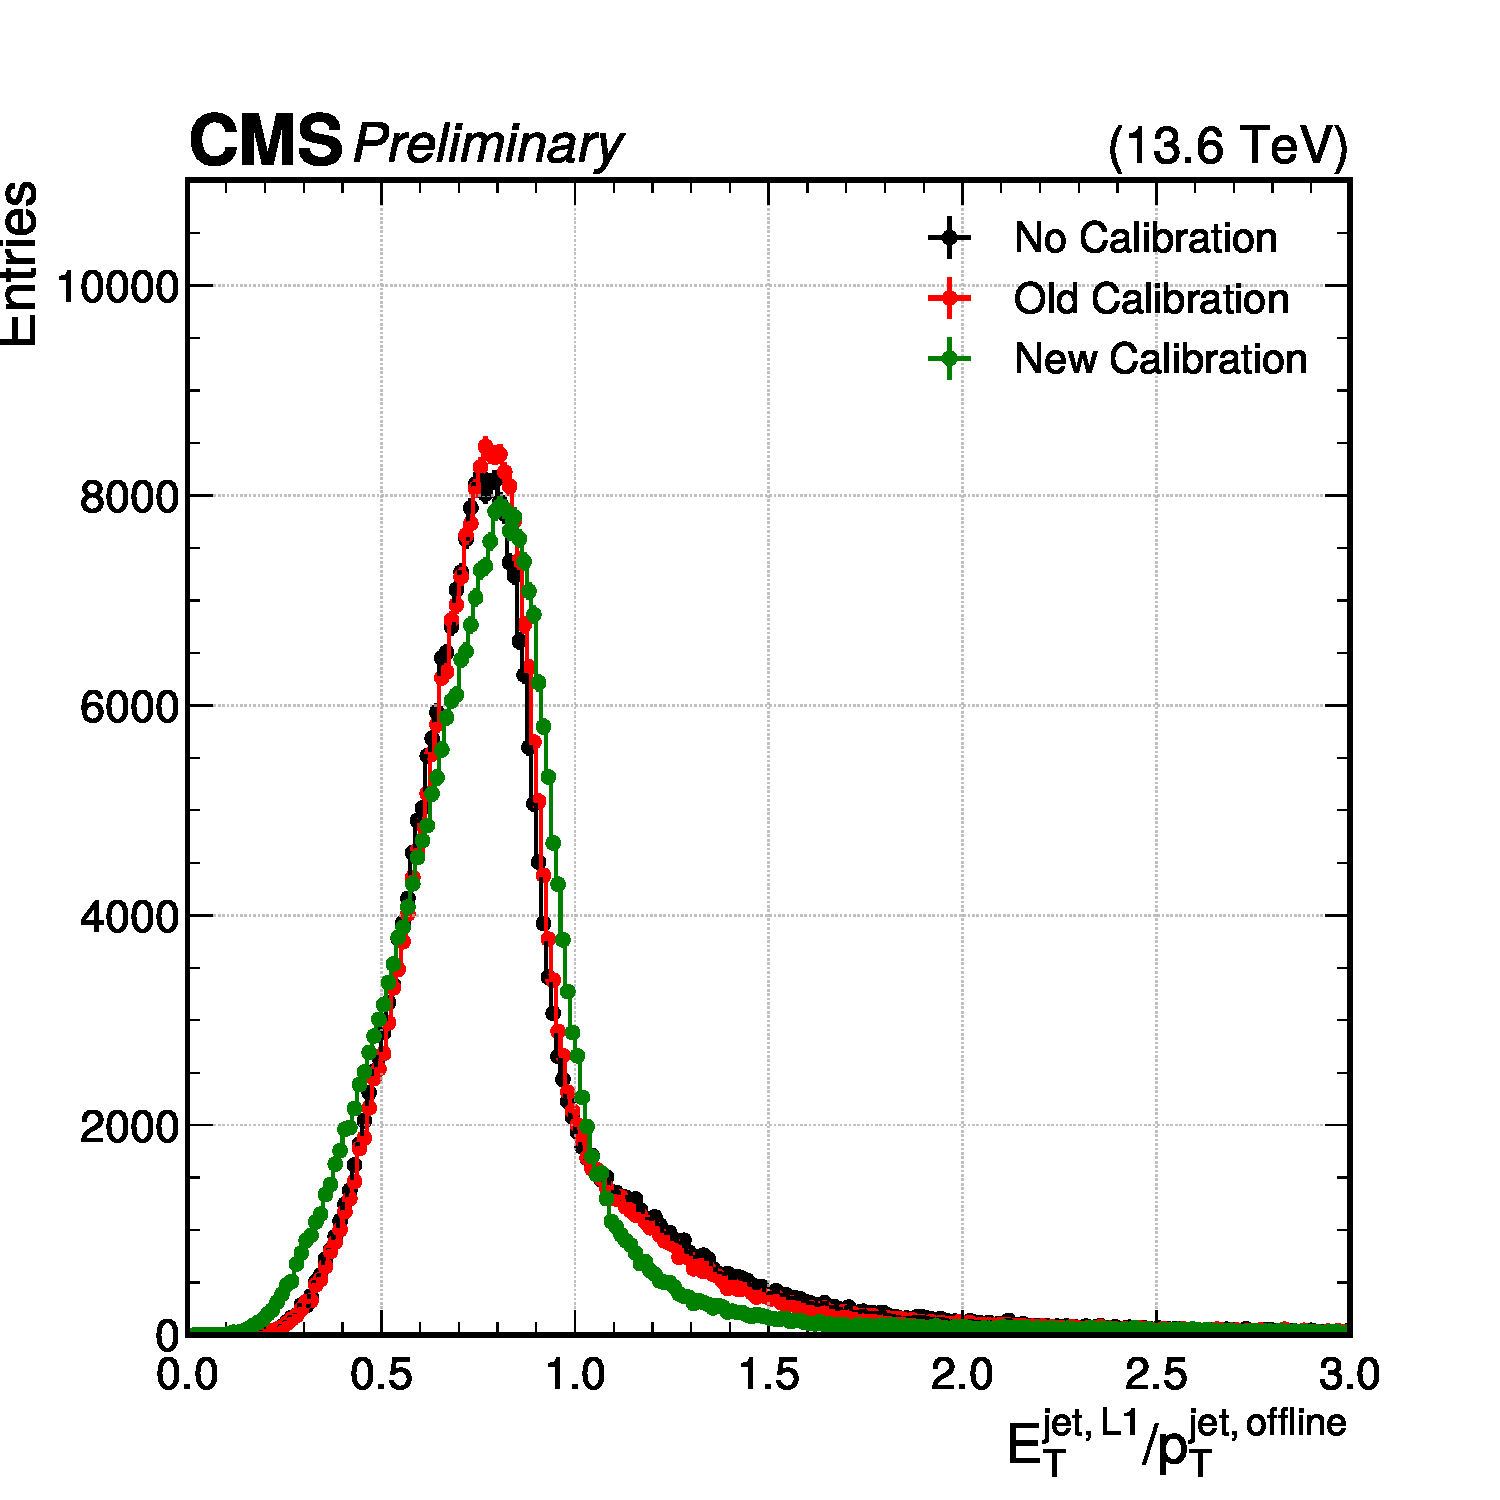
\includegraphics[width=0.5\linewidth]{Figures/L1TP/NN_Performance/response_inclusive__jet.pdf}}
    
    \subfloat[Energy Resolution]{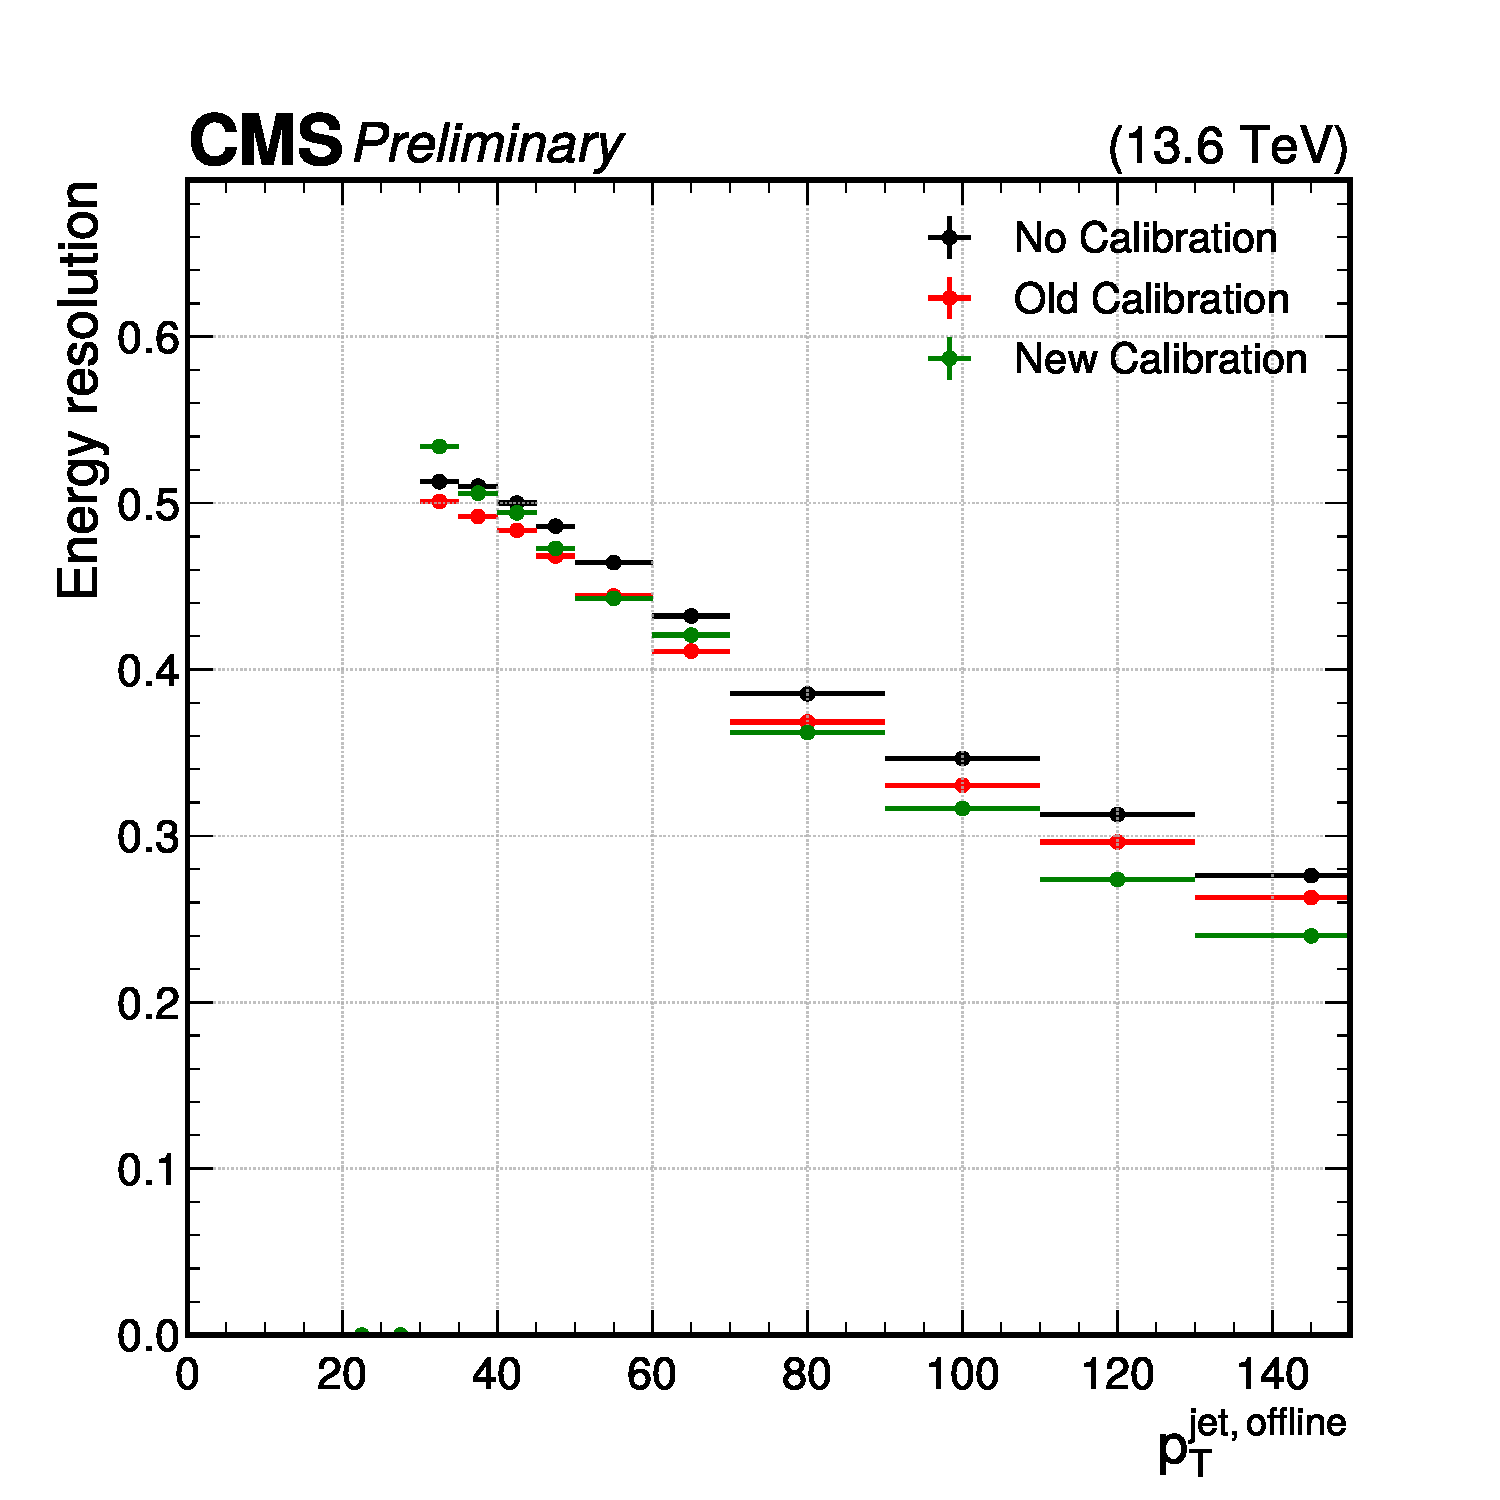
\includegraphics[width=0.5\linewidth]{Figures/L1TP/NN_Performance/resolution_ptBins__jet.pdf}}
    \subfloat[Energy Scale]{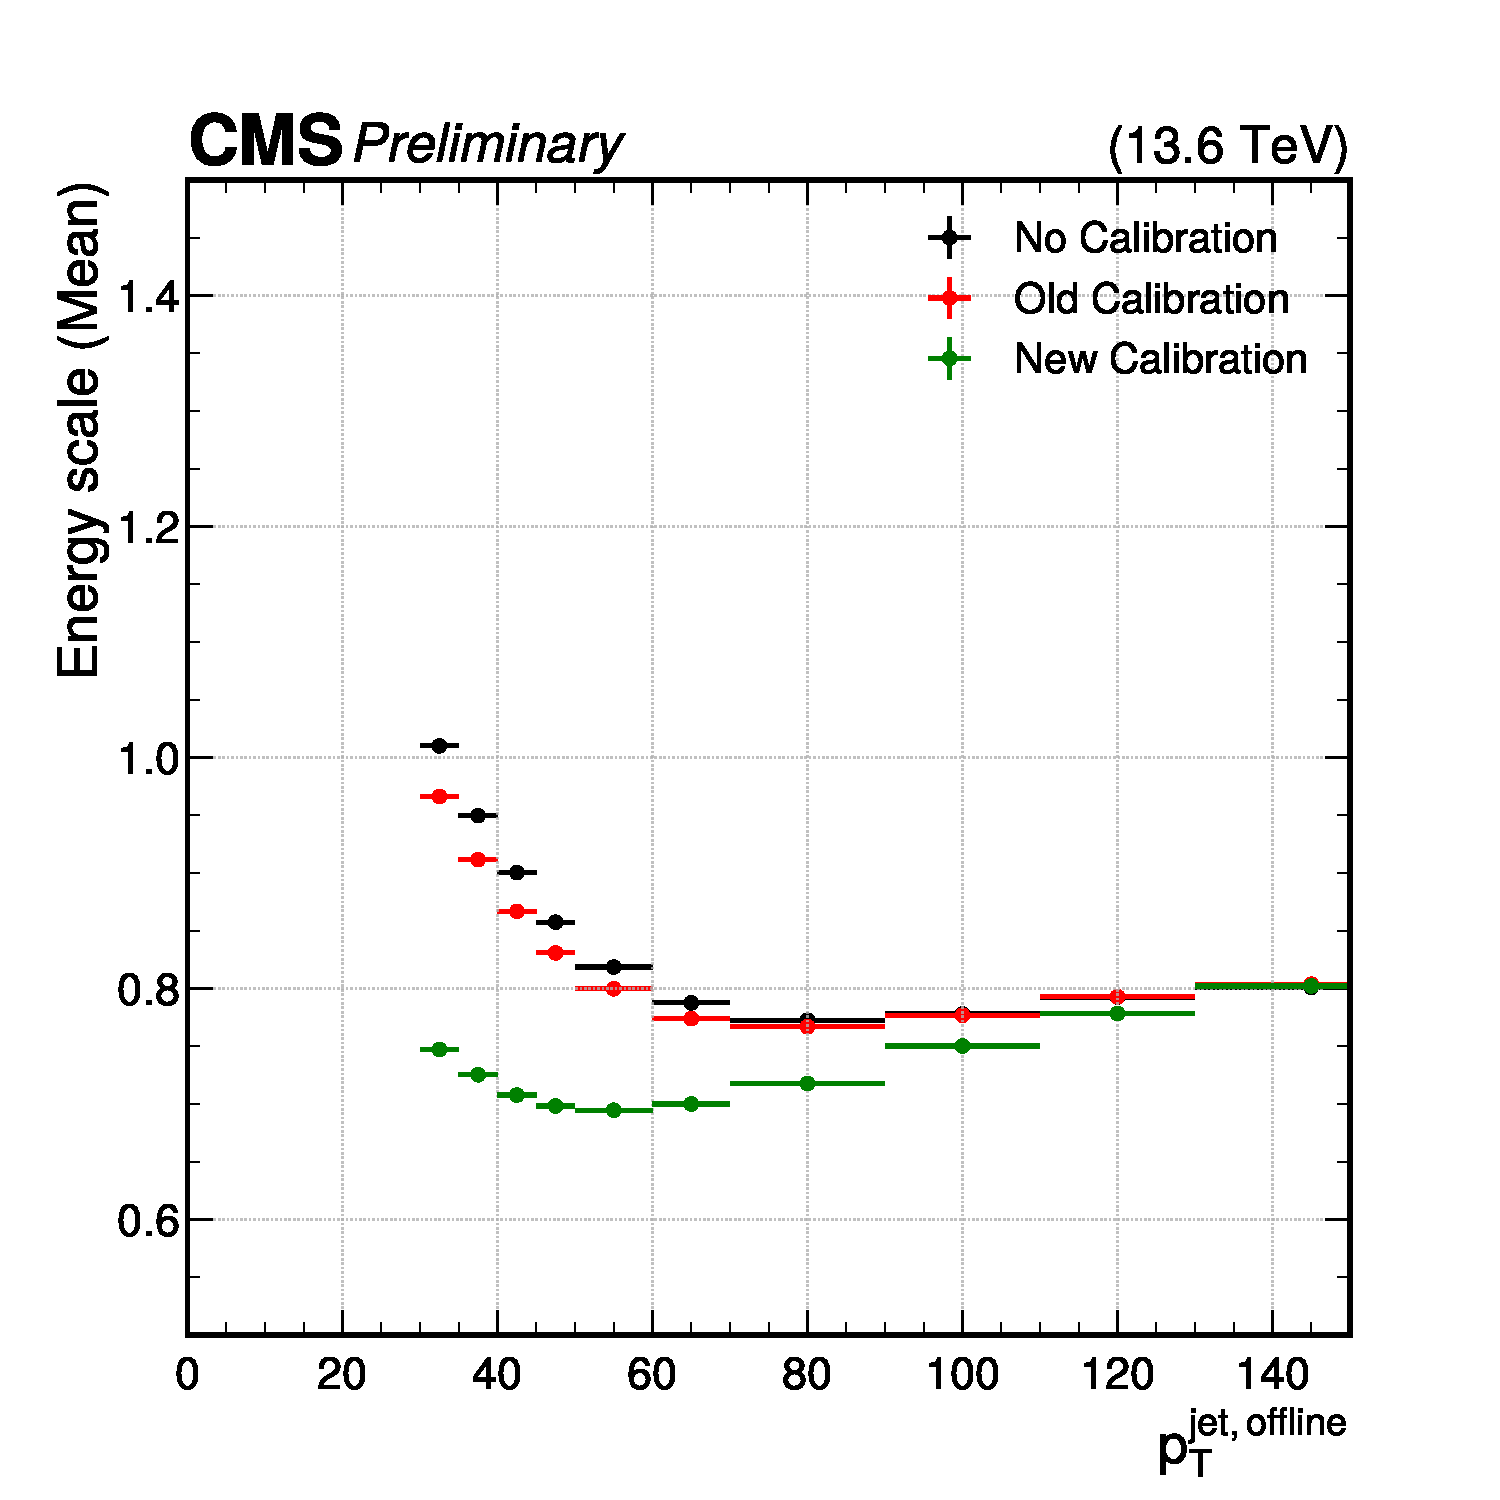
\includegraphics[width=0.5\linewidth]{Figures/L1TP/NN_Performance/scale_ptBins__jet.pdf}}
    \caption{Layer-1 jet performance of the calibration factors derived through the NN approach, in terms of energy response (a), energy resolution (b) and energy scale (c) as a function of the offline $p_T$. The energy of the L1 jet candidate is obtained by replicating the Layer-1 firmware with three different configurations: no calibration (black), old calibration (red), and new NN-based calibration (green); no Layer-2 calibration is applied to the L1 candidate.}
    \label{fig:NN_HCAL_Response}
\end{figure}

\begin{figure}
    \centering
    \subfloat[Rate $|\eta|<2.5$]{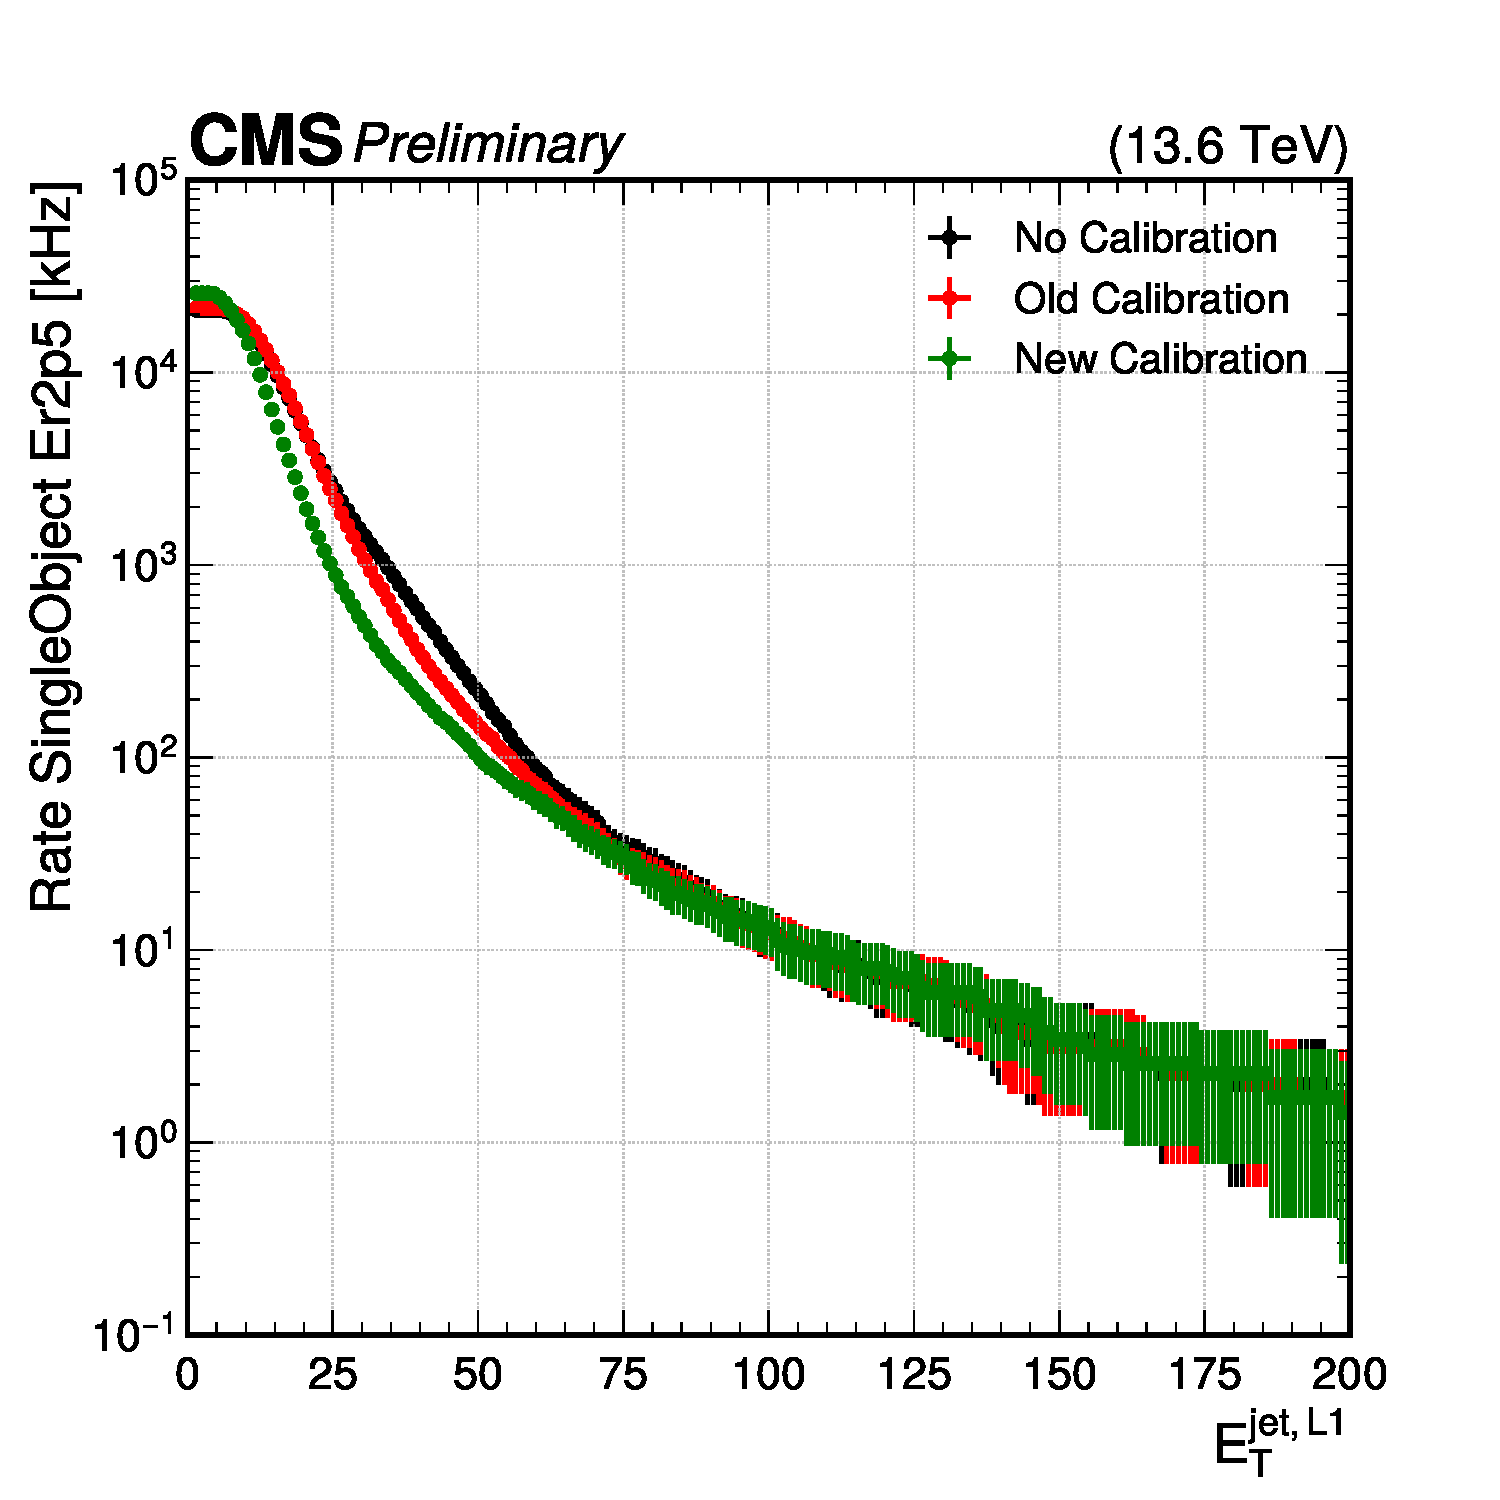
\includegraphics[width=0.5\linewidth]{Figures/L1TP/NN_Performance/rate_ObjEr2p5__jet.pdf}}
    
    \subfloat[Efficiency turn-on $|\eta|<2.5$: $p_T>40$~GeV]{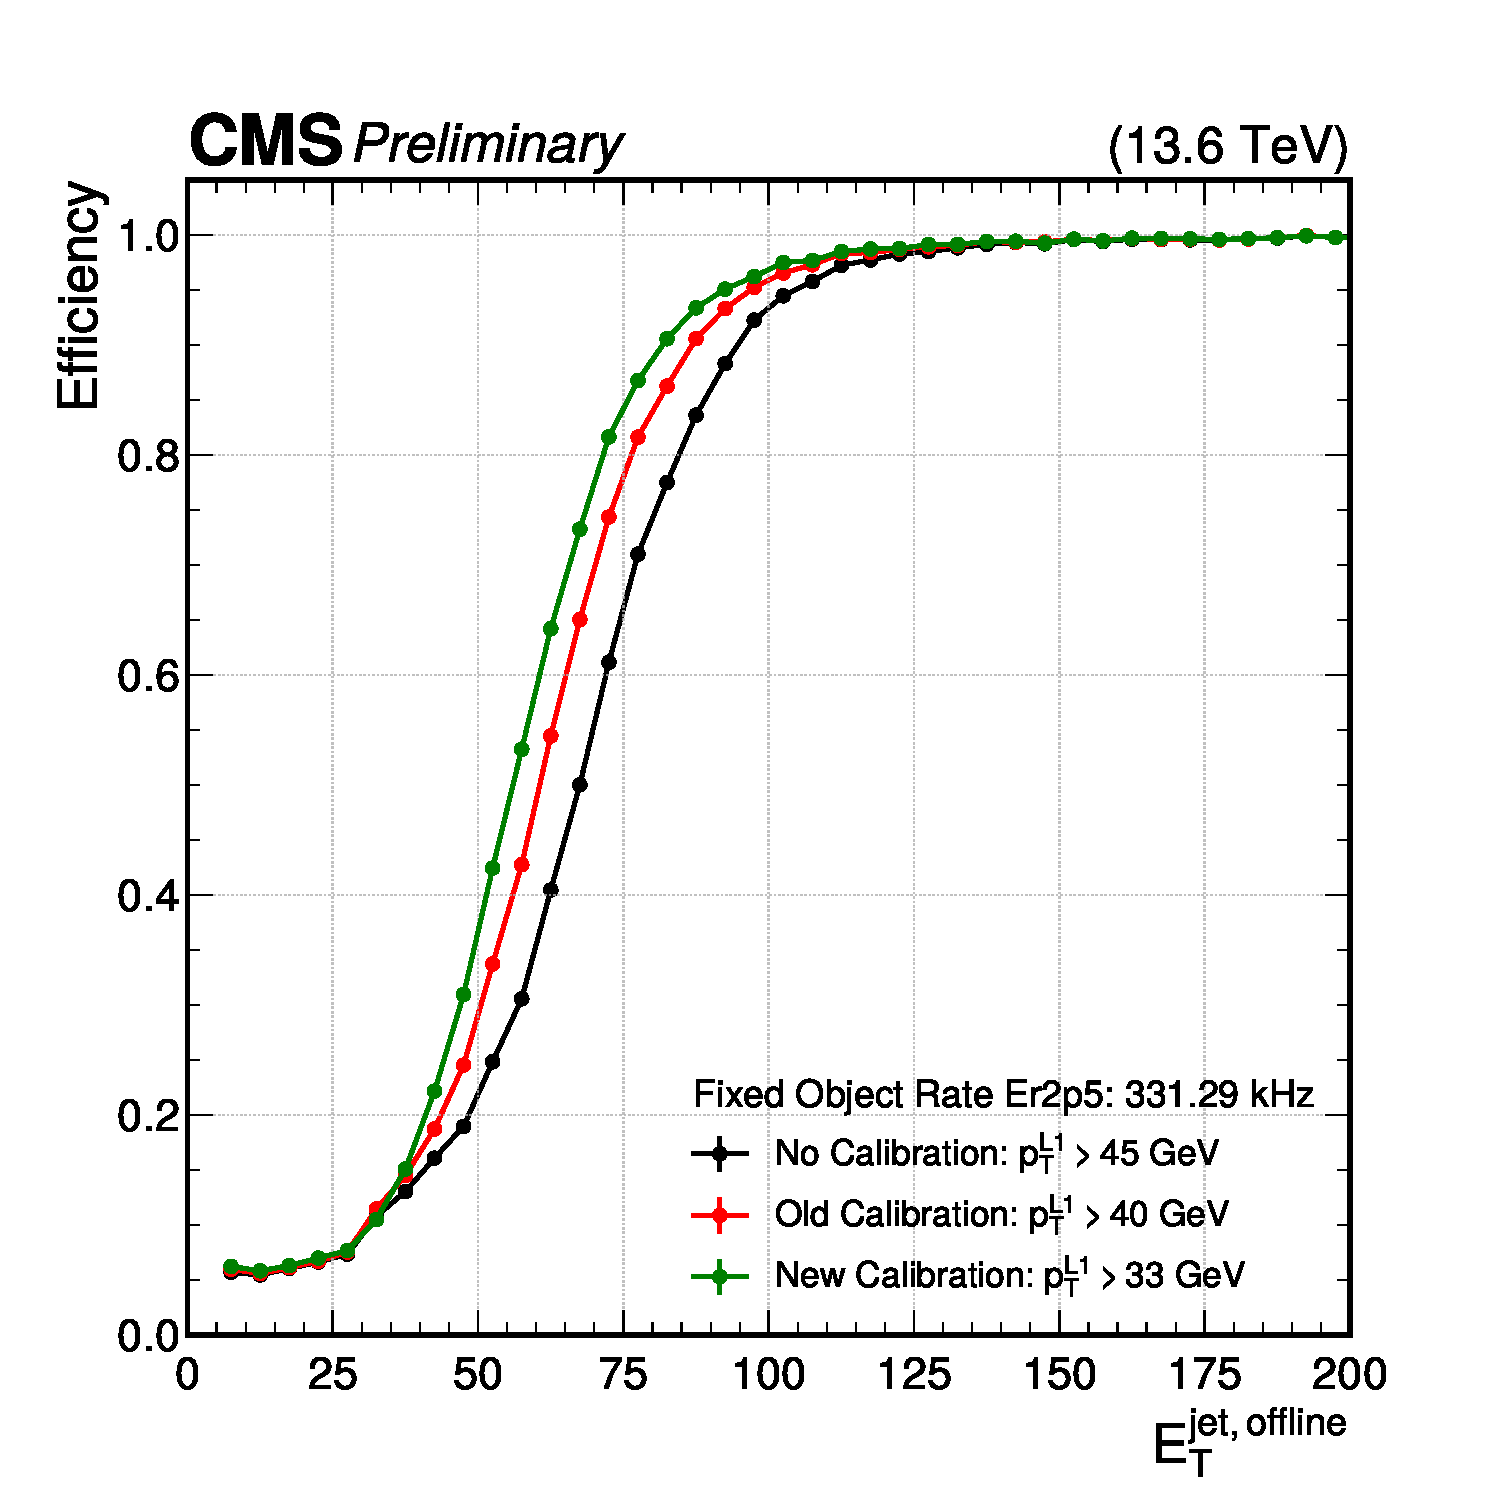
\includegraphics[width=0.5\linewidth]{Figures/L1TP/NN_Performance/turnon_fixedObjRateEr2p5_40__jet.pdf}}
    \subfloat[Efficiency turn-on $|\eta|<2.5$: $p_T>60$~GeV]{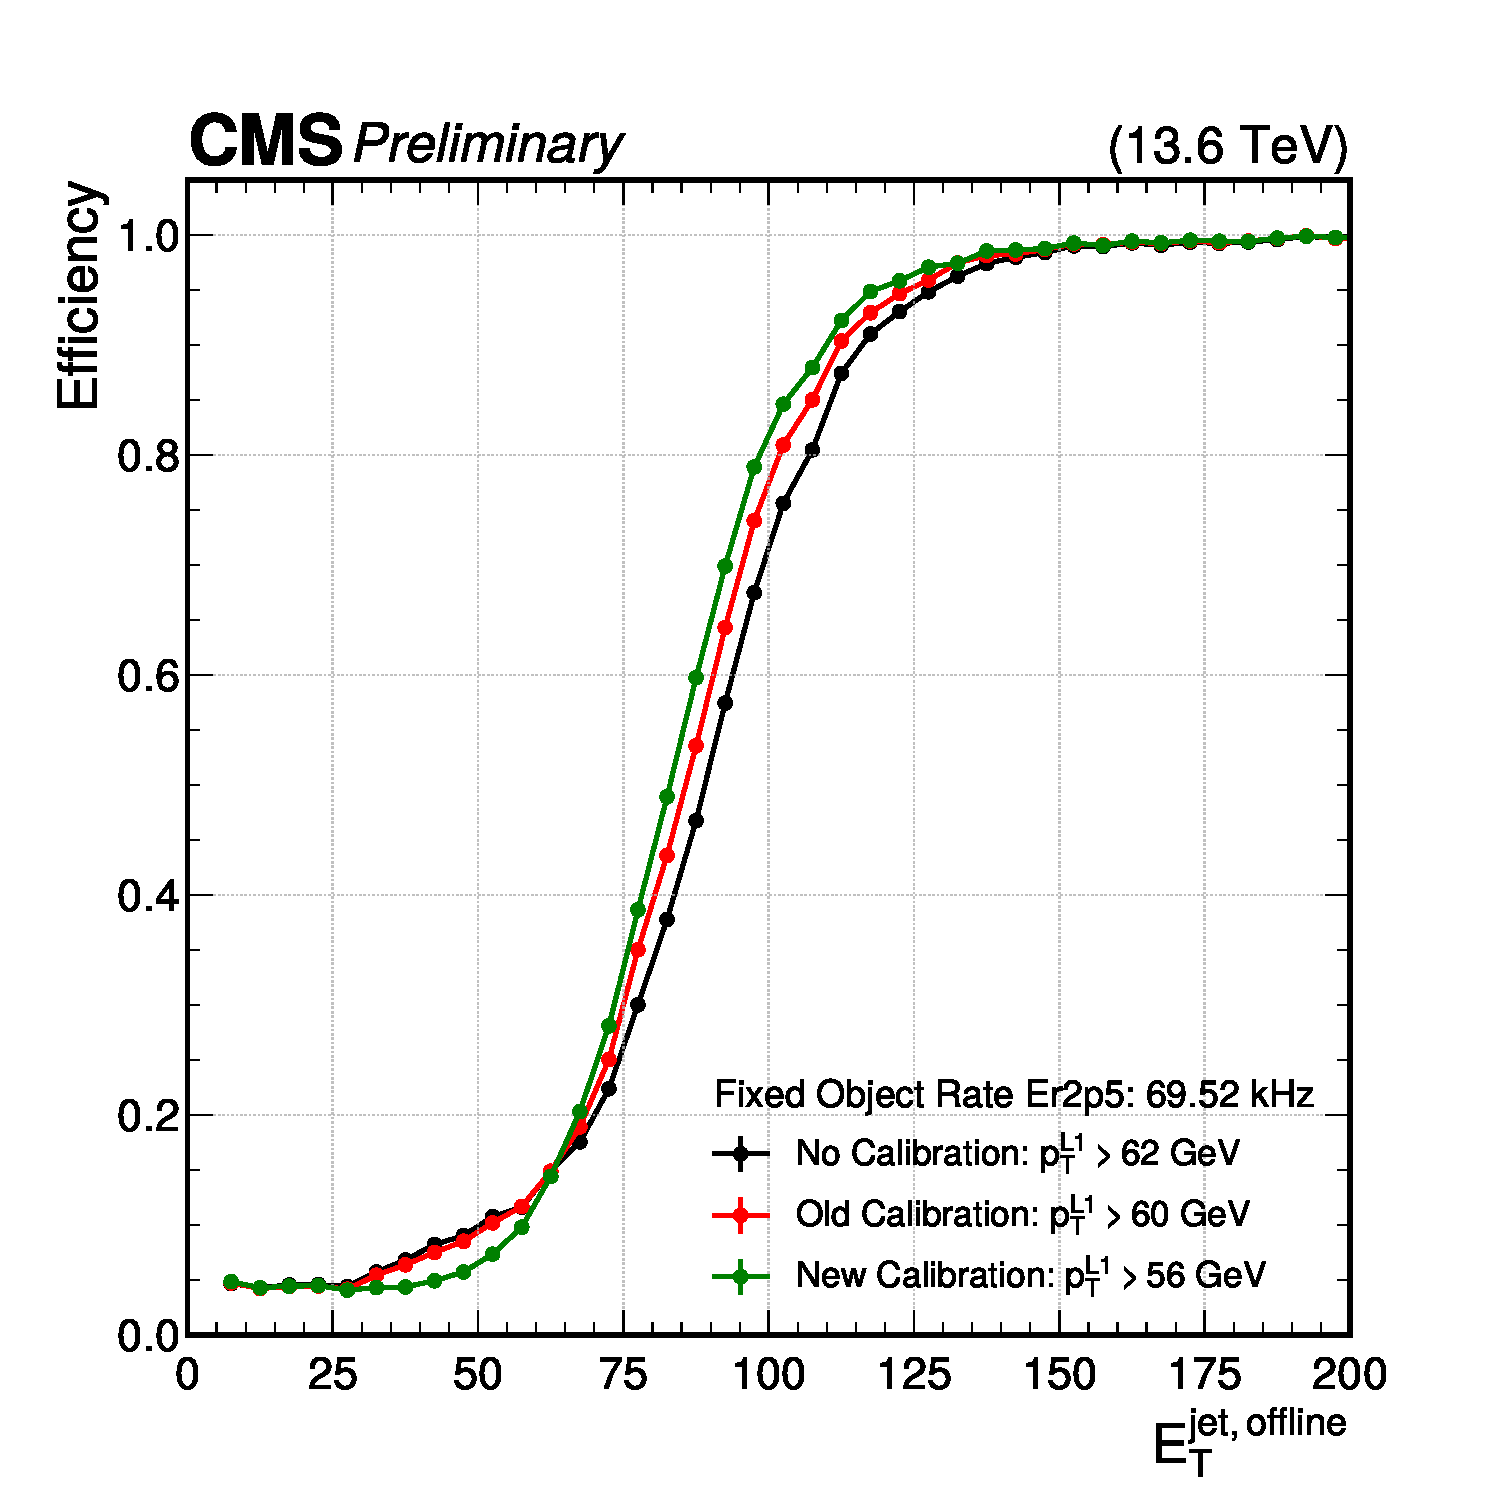
\includegraphics[width=0.5\linewidth]{Figures/L1TP/NN_Performance/turnon_fixedObjRateEr2p5_60__jet.pdf}}
    \caption{Layer-1 jet performance of the calibration factors derived through the NN approach, in terms of rate (a) and efficiency turn-on curves (b-c) for two fixed rate thresholds, to guarantee a fair comparison among different Layer-1 configurations. The energy of the L1 jet candidate is obtained by replicating the Layer-1 firmware with three different configurations: no calibration (black), old calibration (red), and new NN-based calibration (green); no Layer-2 calibration is applied to the L1 candidate. The $|\eta|<2.5$ region is considered, since a vast number of jet trigger seeds only consider this pseudorapidity region.}
    \label{fig:NN_HCAL_TurnOn_ER2p5}
\end{figure}

\begin{figure}
    \centering
    \subfloat[Rate]{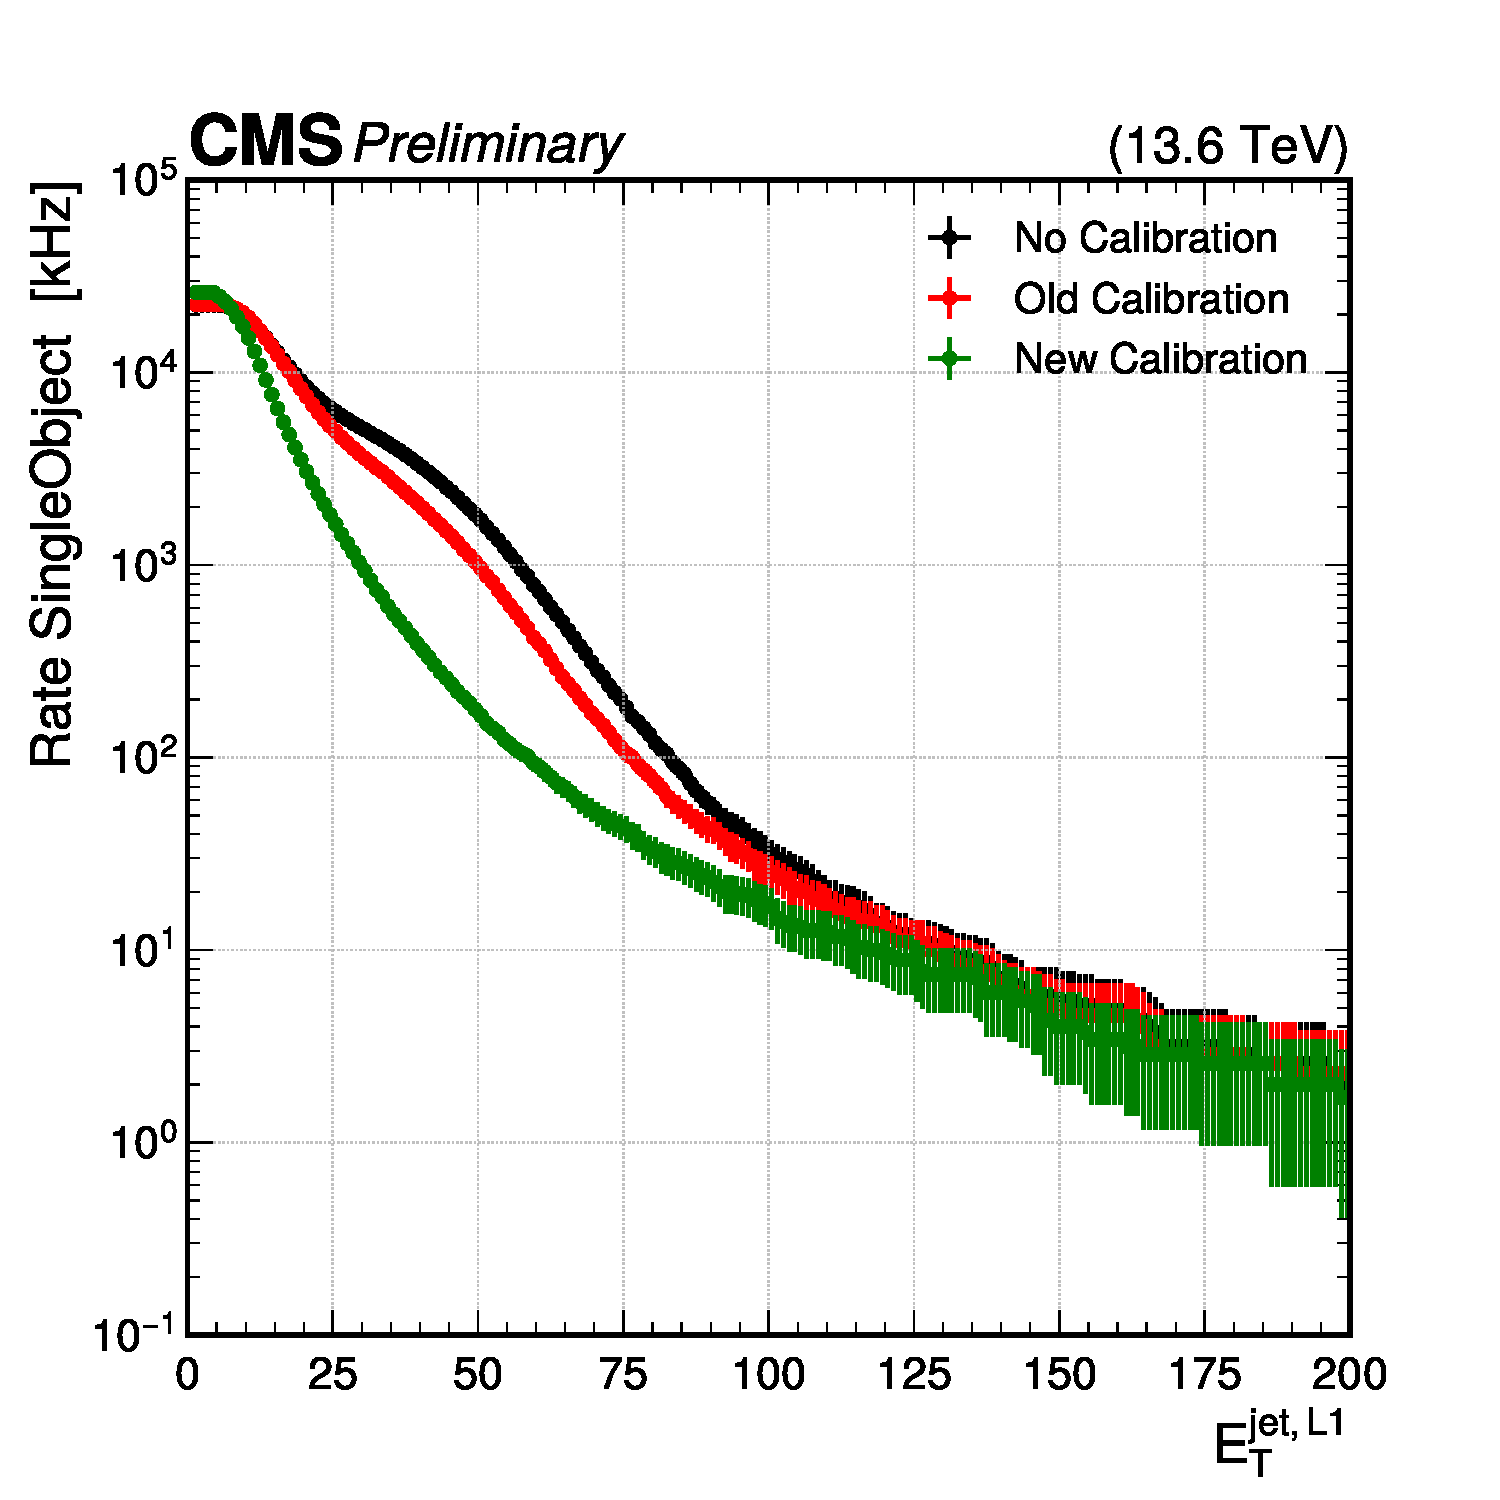
\includegraphics[width=0.5\linewidth]{Figures/L1TP/NN_Performance/rate_Obj__jet.pdf}}
    
    \subfloat[Efficiency turn-on: $p_T>60$~GeV]{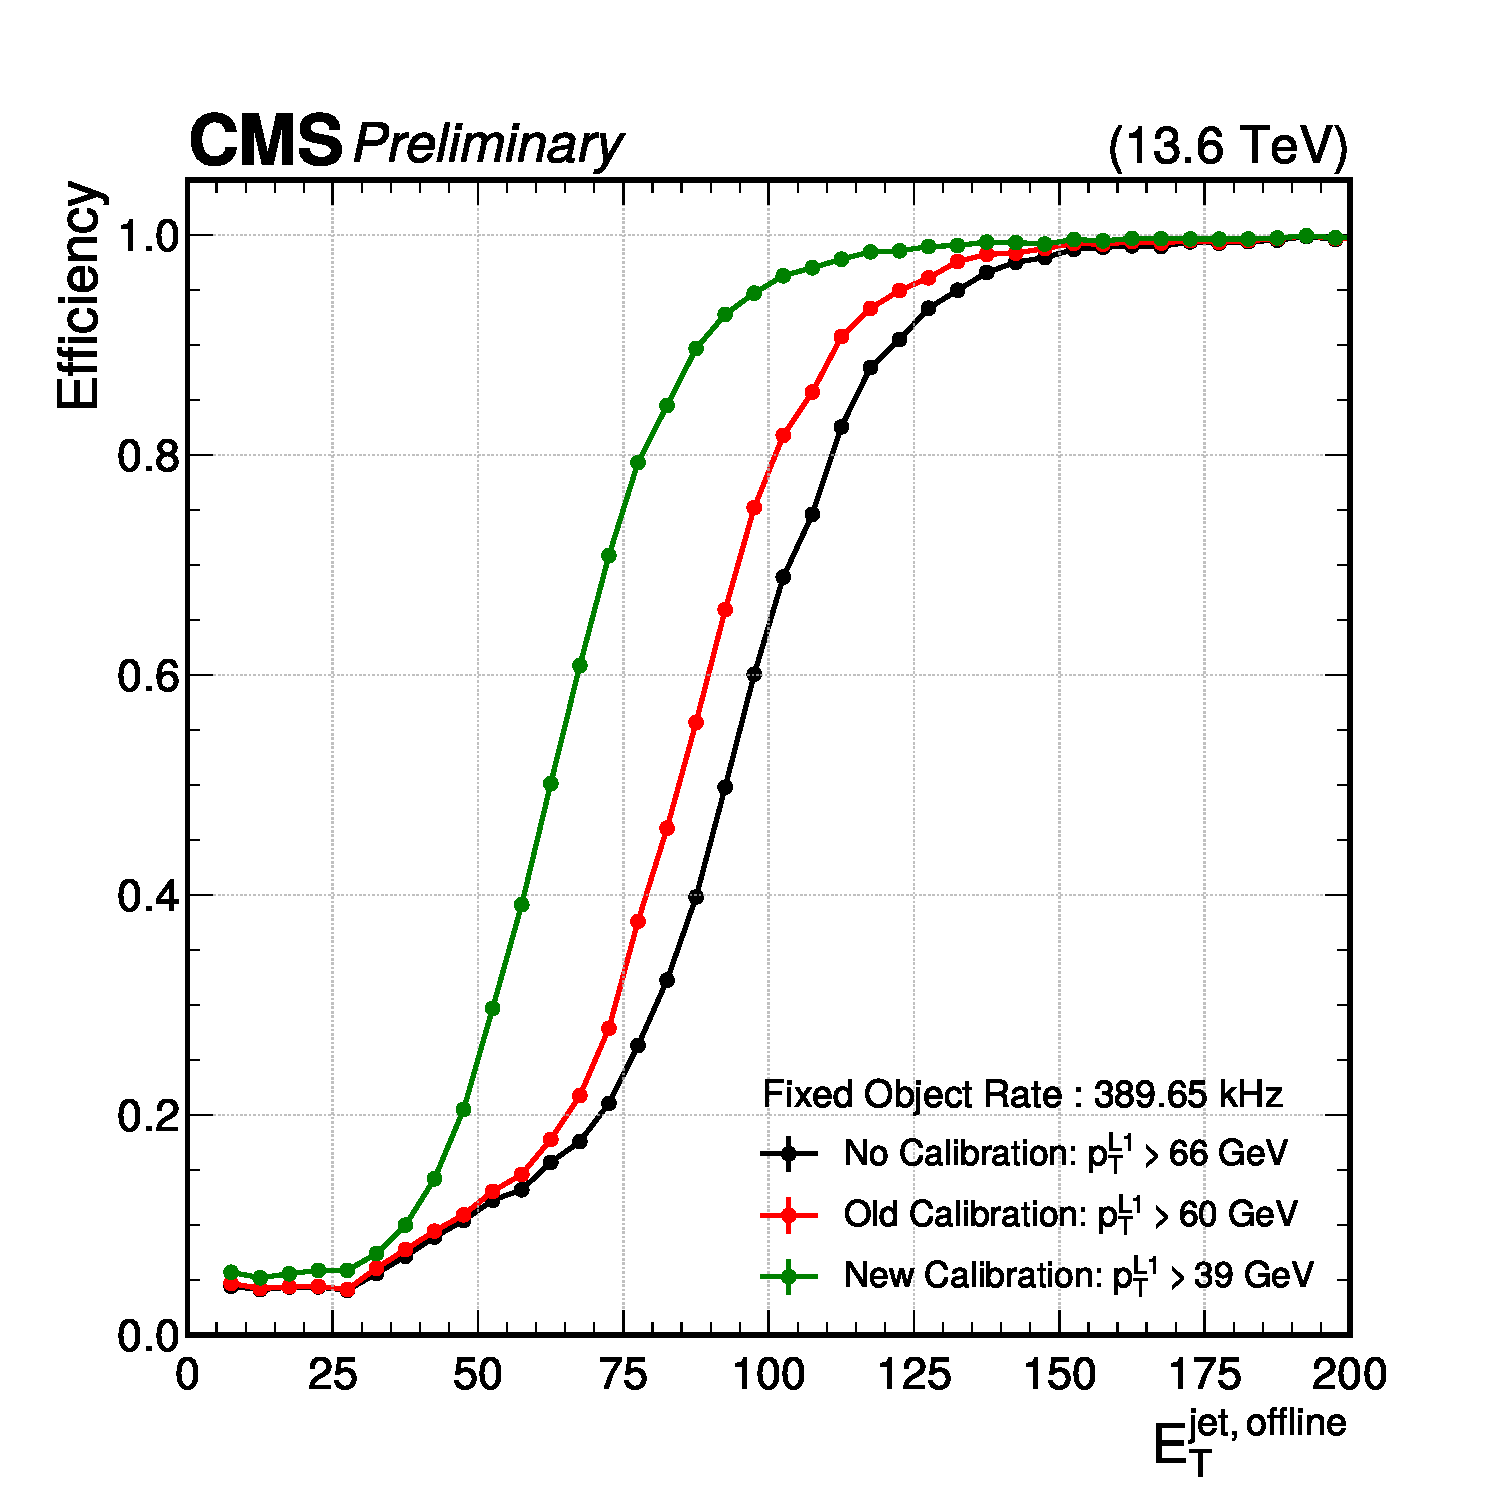
\includegraphics[width=0.5\linewidth]{Figures/L1TP/NN_Performance/turnon_fixedObjRate_60__jet.pdf}}
    \subfloat[Efficiency turn-on: $p_T>80$~GeV]{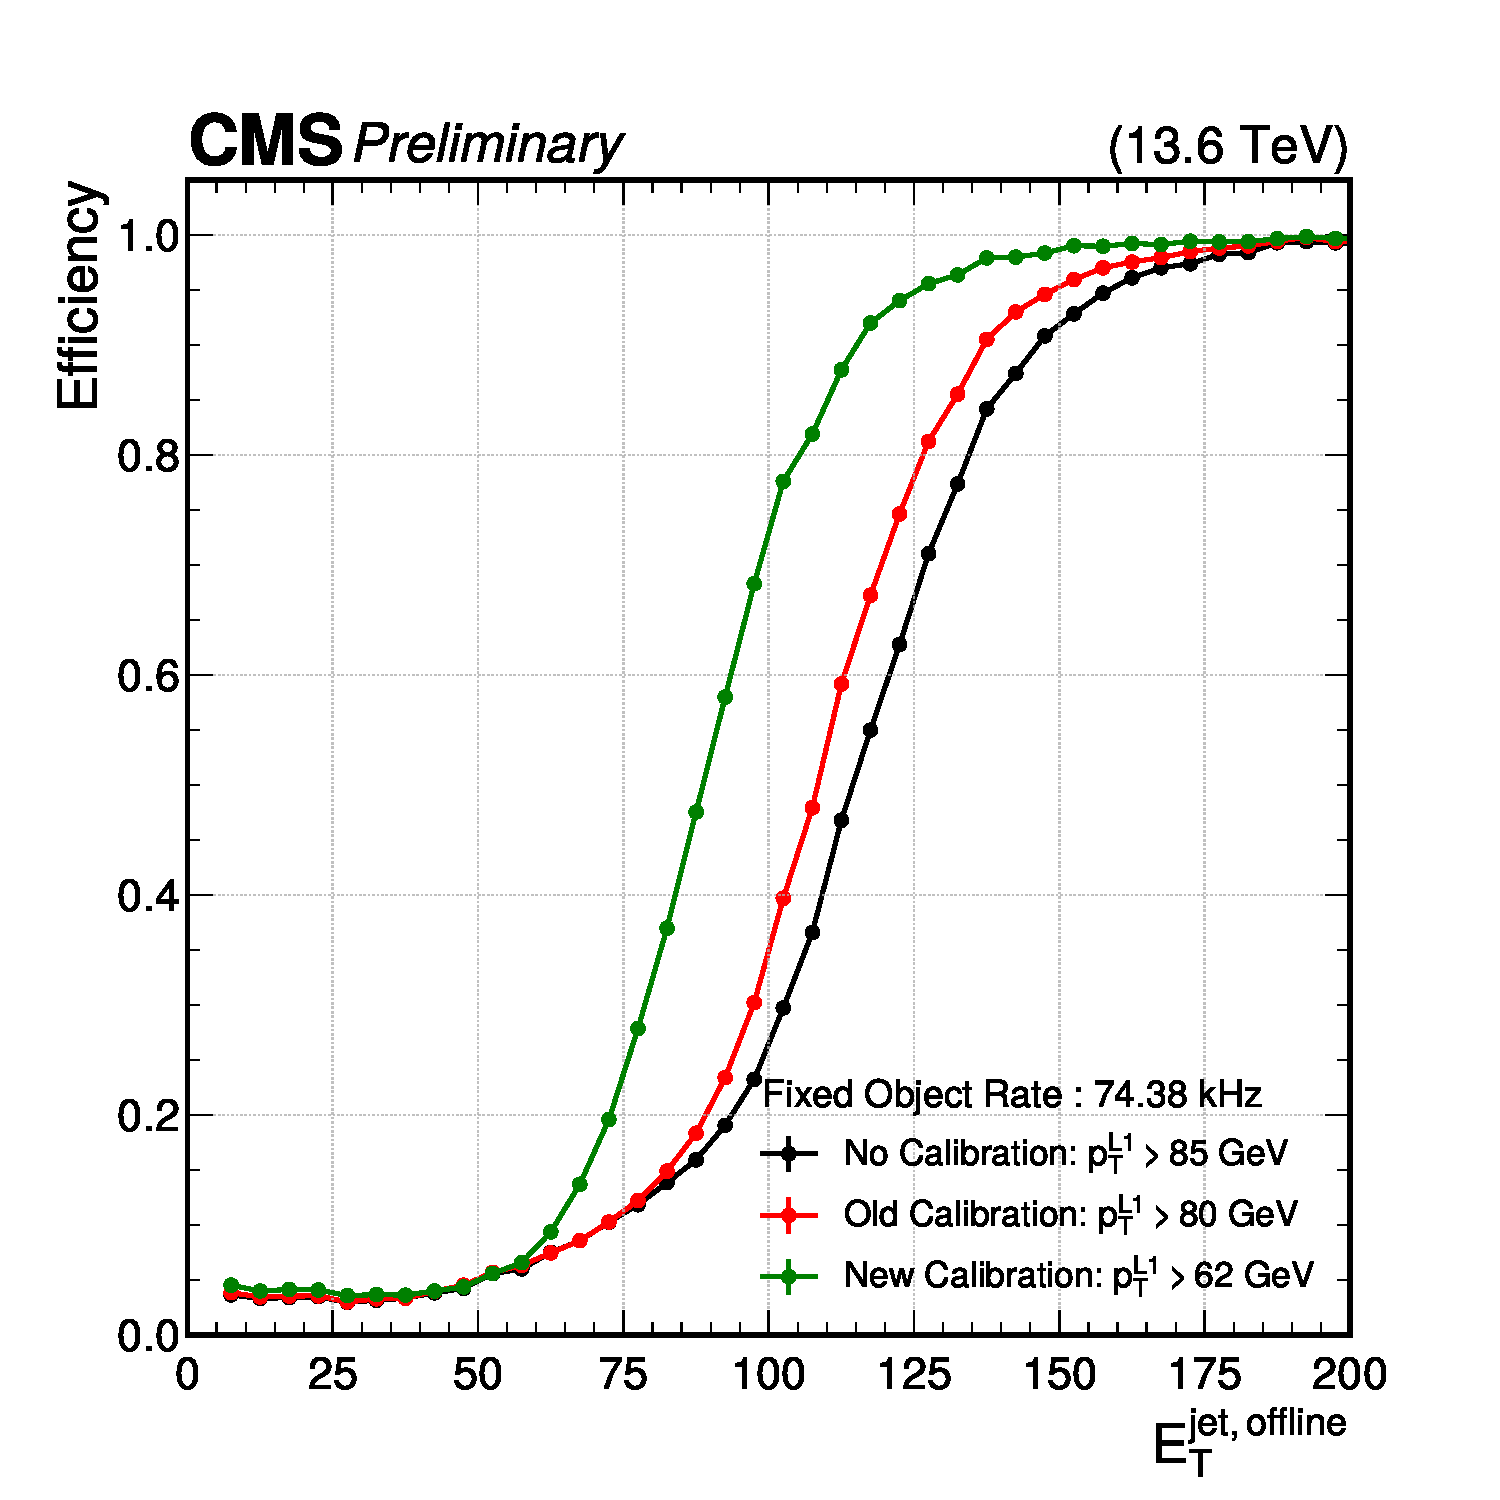
\includegraphics[width=0.5\linewidth]{Figures/L1TP/NN_Performance/turnon_fixedObjRate_80__jet.pdf}}
    \caption{Layer-1 jet performance of the calibration factors derived through the NN approach, in terms of rate (a) and efficiency turn-on curves (b-c) for two fixed rate thresholds, to guarantee a fair comparison among different Layer-1 configurations. The energy of the L1 jet candidate is obtained by replicating the Layer-1 firmware with three different configurations: no calibration (black), old calibration (red), and new NN-based calibration (green); no Layer-2 calibration is applied to the L1 candidate. The full pseudorapidity region is considered.}
    \label{fig:NN_HCAL_TurnOn}
\end{figure}

The ECAL performance is shown in terms of inclusive response, resolution and scale in Figure~\ref{fig:NN_ECAL_Response}. The new NN approach provides a narrower, better centred distribution of the L1 energy response for $e/\gamma$, the resolution is consistently improved across the majority of the $p_T$ range, and the scale is closer to unity. The corresponding Layer-1 expected rate, so as the efficiency turn-on curves for two exemplary fixed rate values are represented in Figure~\ref{fig:NN_ECAL_TurnOn}: the new calibration ensured sharper turn-on curves compared to the old calibration in the low $p_T$ range, while the performance is comparable, or slightly reduced, in the high $p_T$ range.

The HCAL performance of the new NN approach is compared to the other configurations in Figure~\ref{fig:NN_HCAL_Response}, in terms of L1 jet energy response, resolution and scale. The distribution of the response shows comparable performance of the new NN-based scale factors with respect to the other methods: the right tail at higher response is reduced, however there is no significant improvement in terms of resolution or scale. In particular, the reduced scale is driven by the rate term in the loss function, whose relative importance has been optimised in order to provide the optimal efficiency turn-on curve. Figures~\ref{fig:NN_HCAL_TurnOn_ER2p5} and \ref{fig:NN_HCAL_TurnOn} show a performance comparison of the three configurations in terms of rate and efficiency turn-on curves for the inclusive detector response and for the restricted case of $|\eta|<2.5$, where the latter is of particular interest for the L1 trigger performance since a vast number of trigger seeds only consider this pseudorapidity region, less affected by the pile-up activity.
The efficiency turn-on curves show an impressive improvement coming from the NN approach, with reduced rate and better centred turn-on curves: this result is mainly driven by the impact of the new calibration factors on the rate rather than an improvement on the resolution, which is comparable to the old method.

\bigbreak

The performance presented for the NN approach are the result of a careful optimisation of the NN hyper-parameters, conducted by scanning different values for the loss parameters and for the definition of the network architecture. Figure~\ref{fig:NN_HyperParameters} shows the effect of a variation of $C$ and $D$ parameters in the loss function, regulating the importance of the rate term: the results clearly show the competitive effect between a better resolution and a lower rate. Among the different configurations, the one providing the best efficiency turn-on curve is preferred.

\begin{figure}
    \centering
    \subfloat[]{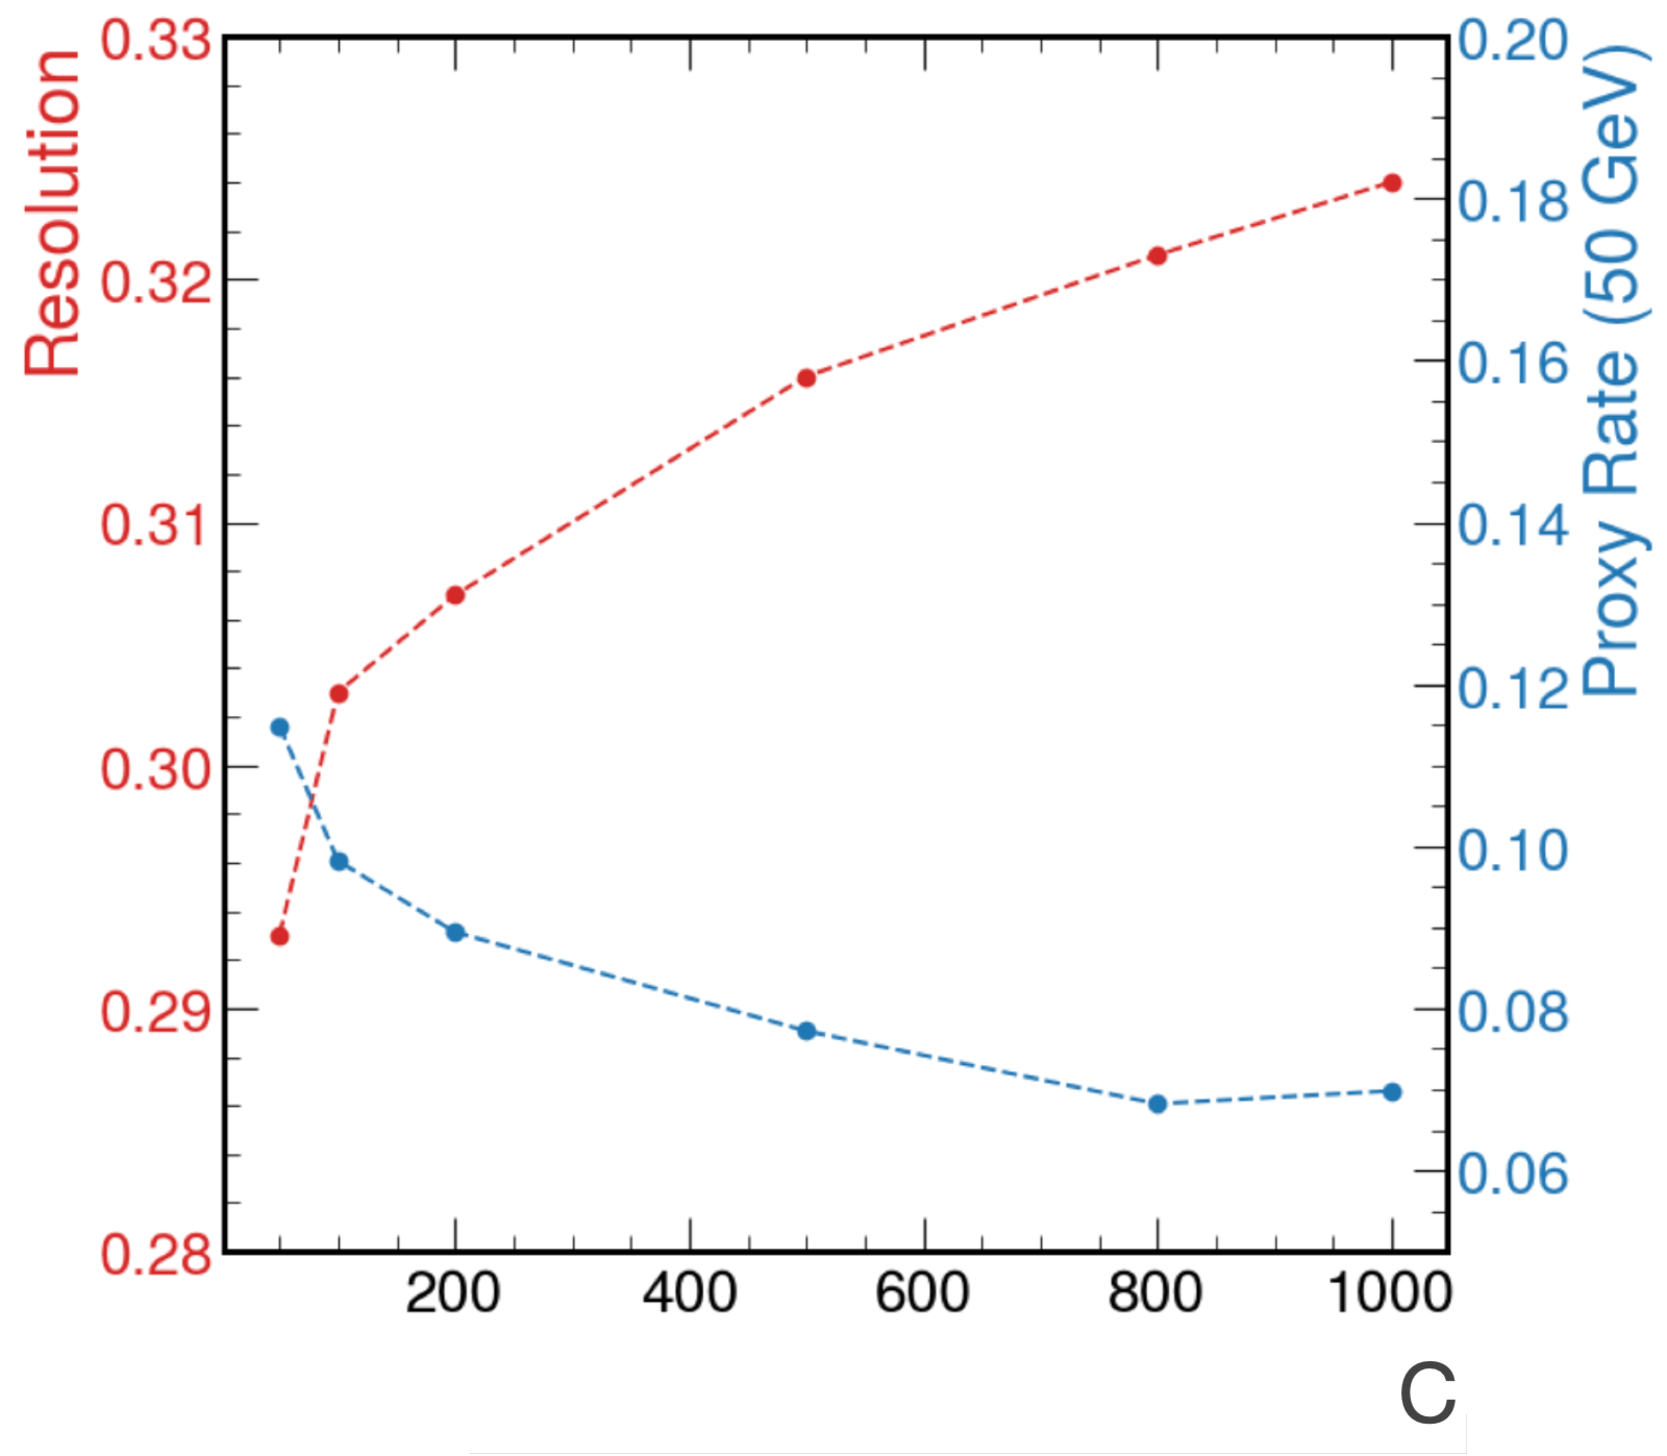
\includegraphics[width=0.4\linewidth]{Figures/L1TP/NN_ParameterC.pdf}}
    \hspace{1cm}
    \subfloat[]{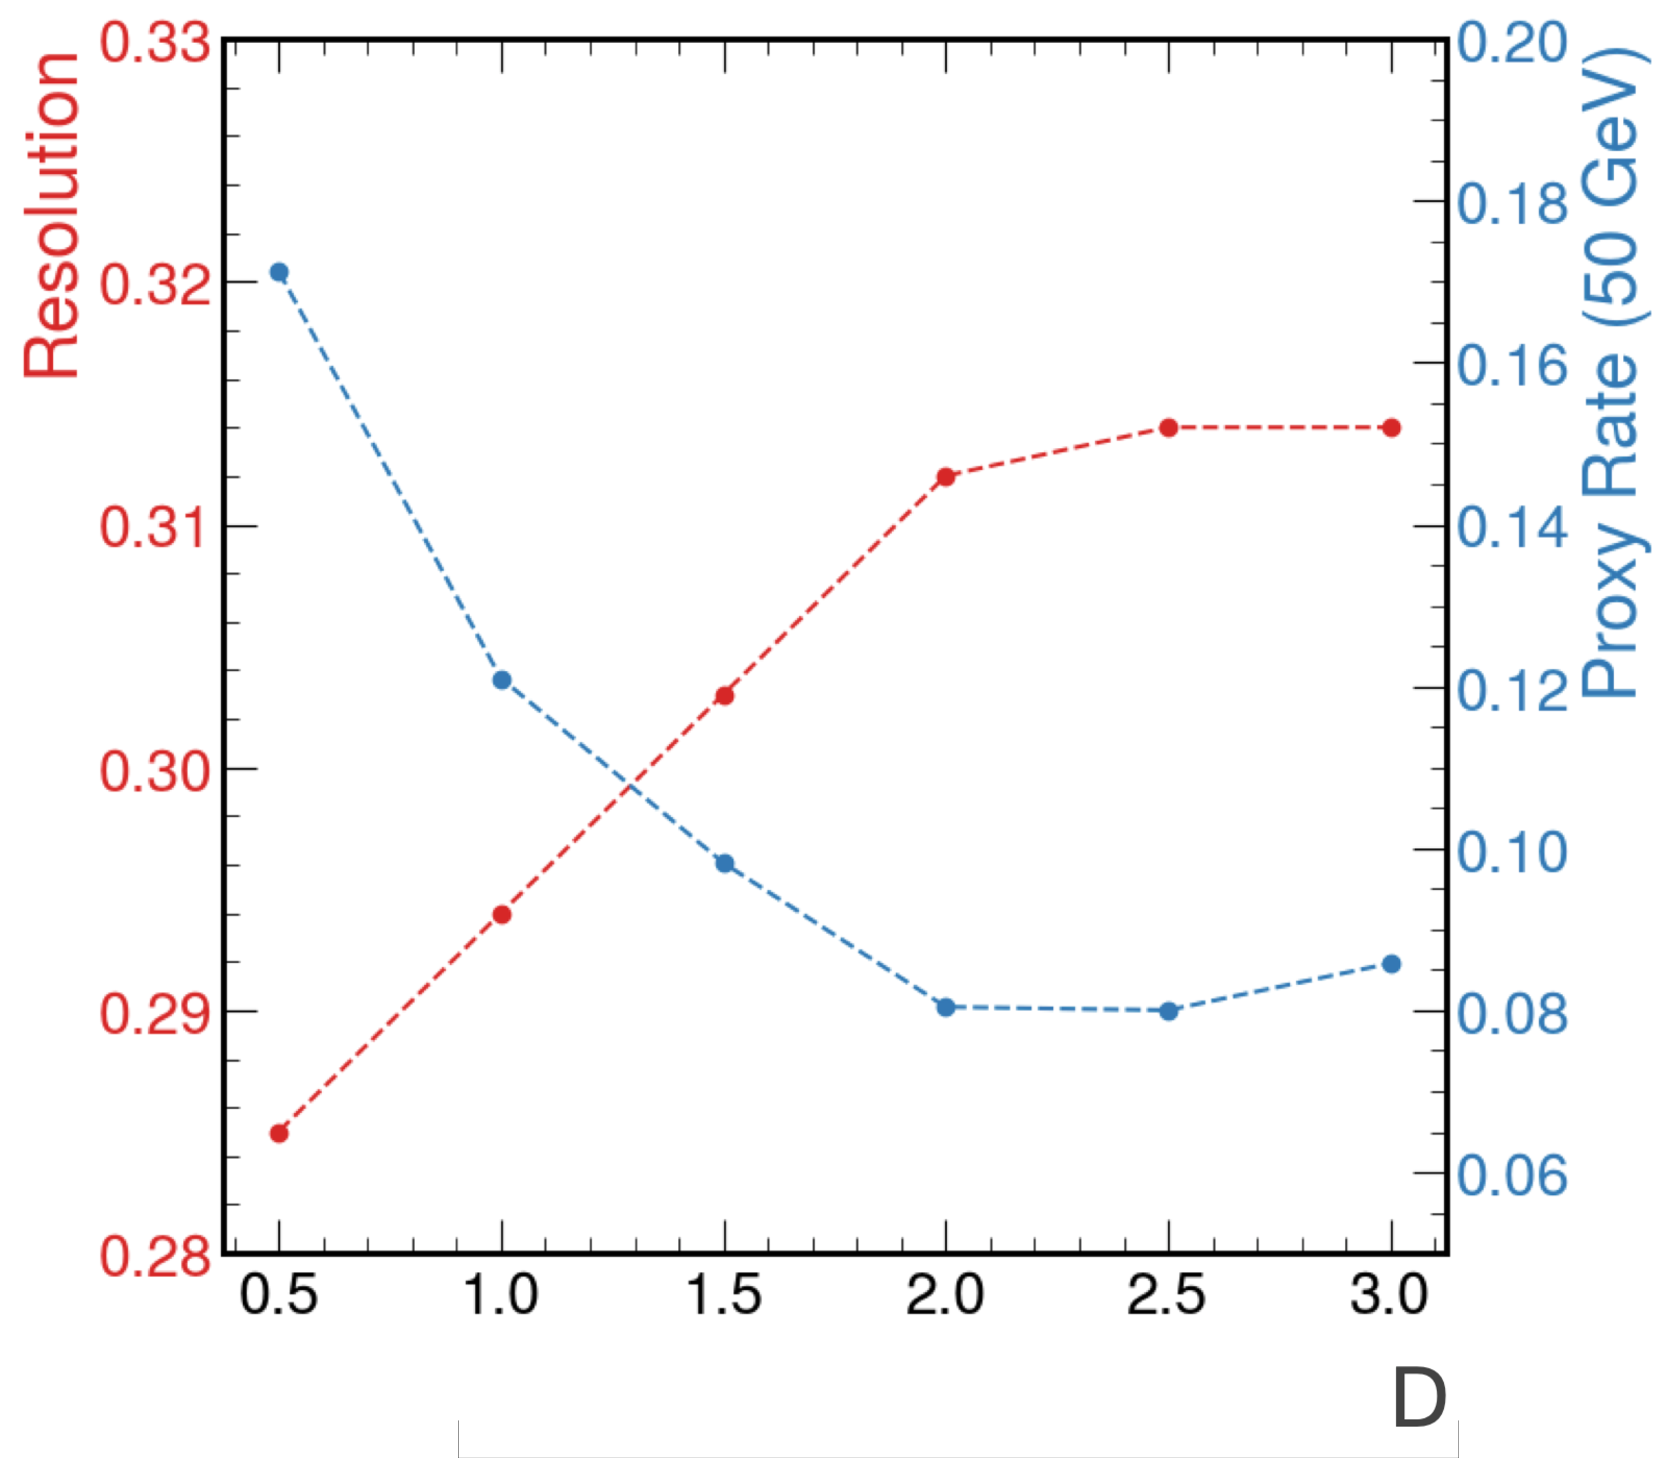
\includegraphics[width=0.4\linewidth]{Figures/L1TP/NN_ParameterD.pdf}}
    \caption{Example of hyper-parameter scanning, for the $C$ (a) and $D$ (d) parameters in the loss function, regulating the importance of the rate term. The values for the expected energy resolution and jet rate proxy are reported: by increasing the importance of the rate term in the loss, the expected Layer-1 rate is reduced, but the new configuration has also a negative effect on the energy resolution, cancelling the gain from a reduced rate.}
    \label{fig:NN_HyperParameters}
\end{figure}

\subsection{Limitations of the Neural Network approach}

Once the new calibration factors have been extracted, and their performance has been evaluated at Layer-1 and compared to the previous method, the final validation of the Layer-1 configuration must be conducted on Layer-2 objects. 
As detailed in Section~\ref{subsec:The Layer-2 calorimeter objects}, the definition of Layer-2 trigger candidates is performed differently for electrons, hadronic tau leptons, jets, and energy sums, and given the stacked architecture of Layer-1 and Layer-2, changes in the Layer-1 configuration necessitate a re-optimisation of the Layer-2 calibration method. 
In the L1 Trigger community, the Layer-2 objects calibration is performed by dedicated groups and involves the expertise of several specialists; therefore, the new Layer-1 configuration has been preliminarily studied at Layer-2 on hadronic tau leptons, whose calibration is based on a complex procedure and provides a comprehensive validation for both ECAL and HCAL components.

The results of the Layer-2 performance for the new Layer-1 calibration factors obtained through the NN approach are presented in Figure~\ref{fig:NN_Layer2}~(a), in terms of efficiency turn-on curves, for the current (red) and the new (blue) Layer-1 and Layer-2 calibration. The combination of the new NN-based Layer-1 calibration and the Layer-2 re-optimisation results in a less sharp efficiency turn-on curve compared to the current configuration. 
This indicates that the improvement observed at Layer-1 does not directly translate into better Layer-2 performance. The primary reason for this lack of improvement is the degraded isolation efficiency between hadronic tau and jet candidates, due to the over-calibration of low-energy TTs, and represented by the ROC curve in Figure~\ref{fig:NN_Layer2}~(b).
Various configurations were tested, including artificially saturating the Layer-1 calibration factors for low-energy towers to unity. However, this drastic change led to even worse performance, as the calibration no longer reflected the NN-learned patterns and predictions.

\begin{figure}
    \centering
    \subfloat[]{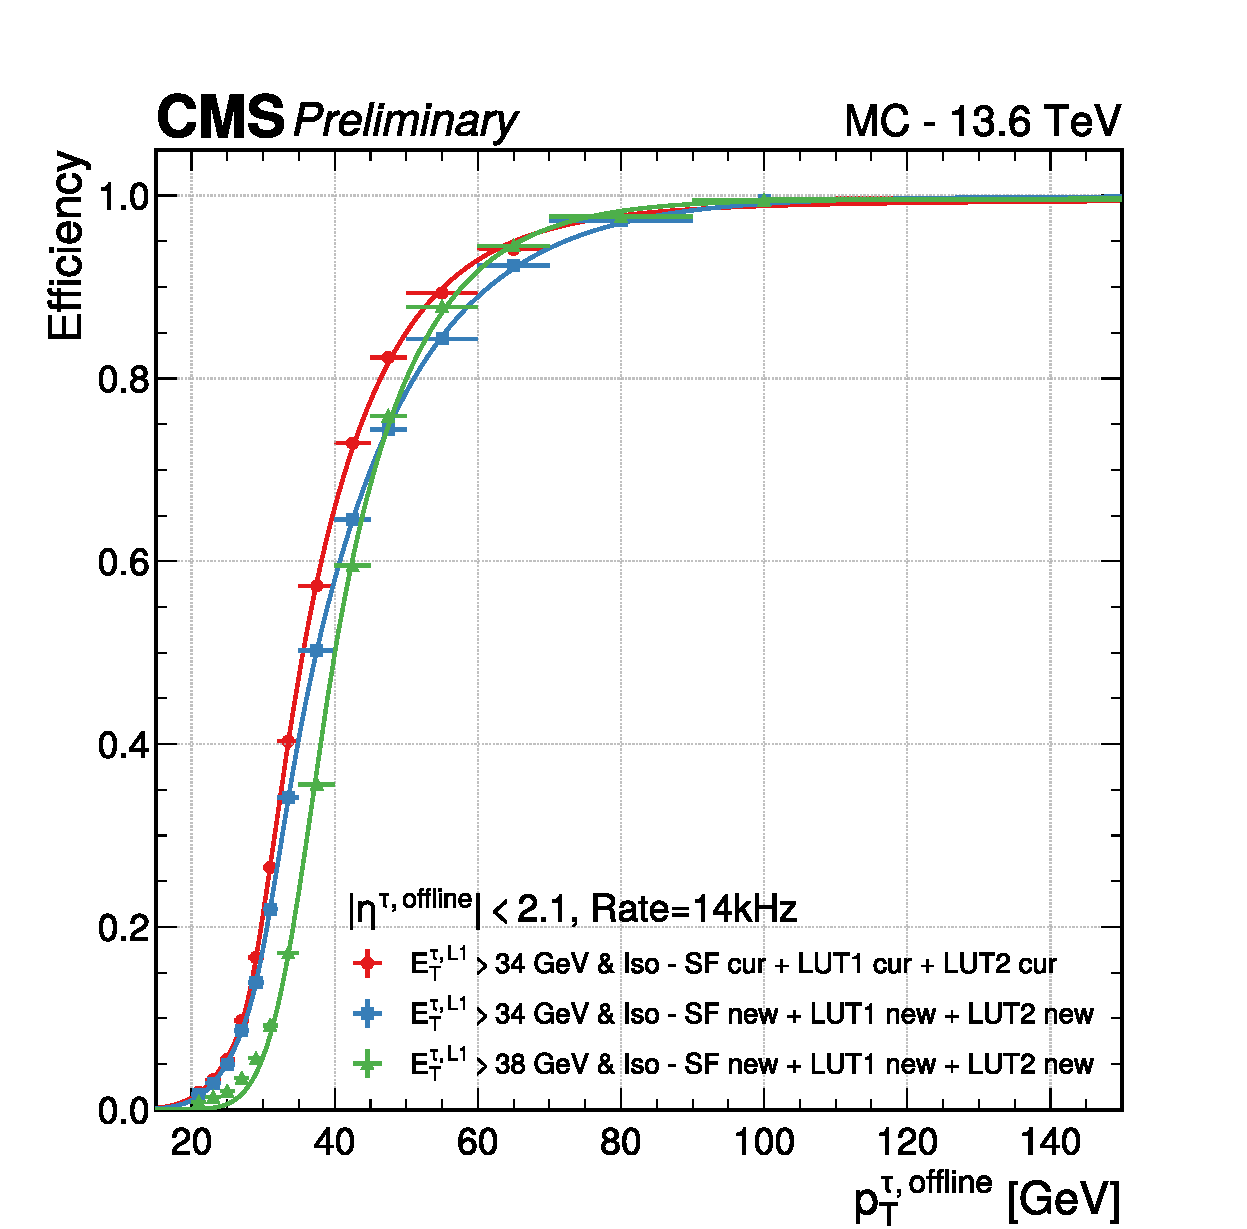
\includegraphics[width=0.45\linewidth]{Figures/L1TP/NN_Layer2_Taus.pdf}}
    \hspace{1cm}
    \subfloat[]{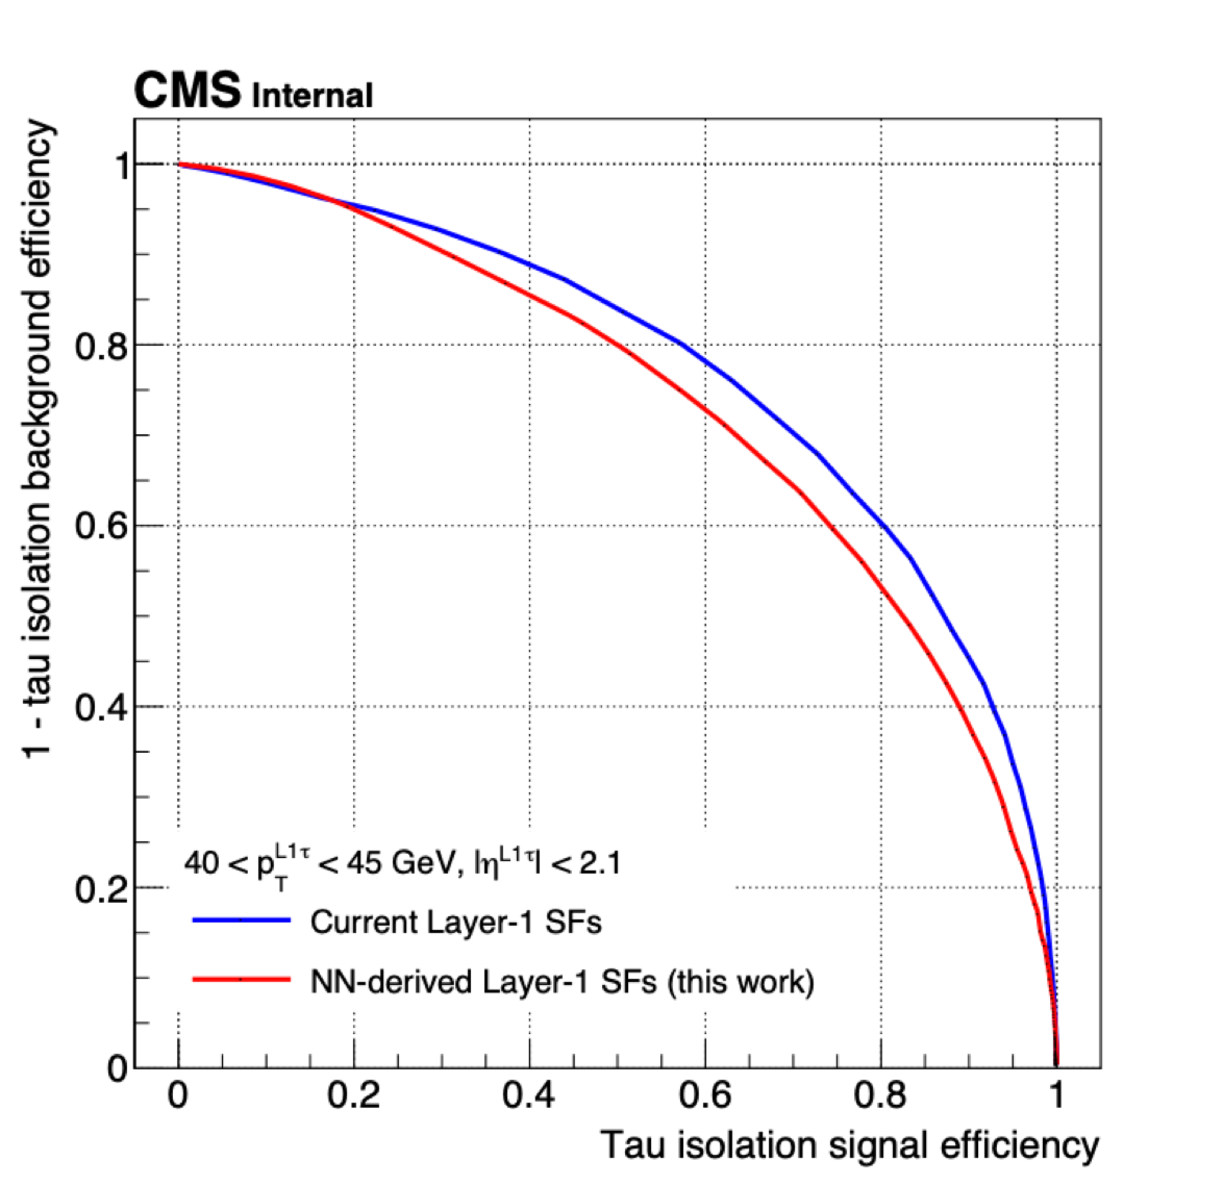
\includegraphics[width=0.45\linewidth]{Figures/L1TP/NN_Layer2_ROC.pdf}}
    \caption{Layer-2 performance of the new NN-based Layer-1 calibration on hadronic tau leptons, compared to the current calibration, in terms of efficiency turn-on curve (a), for fixed threshold (blue vs red) and fixed L1 rate (green vs red). The Layer-2 calibration procedure is re-optimised to account for the different Layer-1 calibration factors. The new NN-based Layer-1 calibration does not provide improvements with respect to the current configuration: the lack of improvement is caused by a degraded isolation efficiency between hadronic tau and jet candidates, represented in terms of ROC curve (b).}
    \label{fig:NN_Layer2}
\end{figure}

\bigbreak

The study on hadronic tau leptons at Layer-2 highlighted the critical importance of a correct interface between Layer-1 and Layer-2, revealing how a better Layer-1 performance does not automatically translate into improved Layer-2 performance. The complex and delicate algorithms for the definition of the L1 candidates are extremely sensitive to changes in the Layer-1 calibration factors, and ad-hoc constraints on individual towers are required directly during the training procedure.
In this context, the NN approach does not provide an ideal environment, given the non-trivial relationship between the network trainable parameters and the physical calibration factor values. 
Moreover, the capability of NNs to interpolate the detector response in energy regions with no input makes the calibration factors less controllable.
% OPTIONAL: example of extrapolation in Zero Suppression region
% OPTIONAL: problem with the rate proxy definition
% OPTIONAL: we use single tower inputs to extract SFs but they are never seen by the NN

For the application of the ML-based calibration method to the Layer-1 context, the NN approach has revealed its limitations. After several attempts, it was decided to adopt a different algorithm for the Layer-1 calibration procedure, allowing for direct customisation of the individual calibration factors and better model interpretability: a proposed technique that facilitates these aspects is the use of JAX library.

\section{The JAX approach} 

In order to overcome the limitations of the NN approach in terms of model interpretability and customisation of the individual calibration factors, the NN algorithm has been substituted by a new differentiable programming approach based on JAX~\cite{jax2018github}, a Python library designed for accelerator-oriented array computation and high-performance program transformation.
In the new implementation, the trainable parameters are no longer encoded in the NN hidden layers, the calibration factors are explicitly defined as a matrix of weights to be applied to the TTs in input, and their values can be individually constrained during the training procedure.

The basic technique for the model training and the extraction of Layer-1 calibration factors remains unchanged with respect to the NN approach. The JAX calibration techniques applies the logic presented in Equation~\ref{eq:Training}: the input to the JAX algorithm is the raw energy deposit $E_T$ and $i\eta$ position of each TT composing the L1 candidate, and the calibration factors are applied to each tower in order to obtain a calibrated L1 object energy as close as possible to the offline reference value. 
The main difference comes from the calibration factors definition. In the NN approach, the calibration factors are not explicitly defined in the model, but they are extracted through a standard candle method, by simulating the effect of NN on one-tower inputs. In the JAX architecture, the calibration factors are defined as a fixed-size 2D matrix, where the two dimensions correspond to the $i\eta$ and the raw energy of the TTs.
The calibration factors matrix can be initialised to unity before the training, and the calibration factors corresponding to regions which are not represented in the input datasets are simply not modified with respect to the initial value. This feature is a radical change with respect to the NN approach, where the algorithm was capable of uncontrollably interpolating the calibration factors in regions where no input was available.
Moreover, the individual calibration factors can be easily constrained to pre-defined values, for a better matching with the Layer-2 calibration, by simply masking the learning process of the corresponding matrix element. This procedure has been widely employed for this application, and allows for fine adjustments of specific values, without disrupting the overall calibration pattern. 

The JAX approach provides a simplified model compared to the NN technique, and its implementation does not allow for the extrapolation of non-linear relationships for the model interpolation. However, given the limited information available in the Layer-1 context and the constrained structure of the firmware, the potential non-linearity learnt by the NN model would be cancelled when extracting a single multiplication factor. Therefore, a linear interpolation is sufficient for this application, and better represents the actual Layer-1 firmware structure.

\subsection{The calibration matrix and training procedure}

The JAX calibration algorithm is based on the initial definition of a trainable 2D calibration matrix, containing all the Layer-1 firmware-compatible calibration factors. The $i\eta$ binning follows the detector geometry, i.e. 28 and 41 $i\eta$ positions for the ECAL and HCAL configurations respectively. The energy range is divided into different size bins, with a step of 2~$iE_T$ (1~GeV) for energies below 50~GeV, a step of 10~$iE_T$ (5~GeV) for energies between 25 and 100~GeV, and a single bin from 100~GeV to the saturation energy of 127.5~GeV. The same energy binning is adopted for the extraction of both ECAL and HCAL calibration factors.
This binning choice is motivated by the need of maintaining the high granularity for low-energy towers, where the calibration factors have larger variation, while keeping larger bin size for high-energy towers, where smaller variations are expected.

The 2D calibration matrix ($CM$) can be mathematically expressed as:
\begin{equation}
    \textbf{CM} = \begin{bmatrix} 
    SF_{i\eta_1,iE_1} & SF_{i\eta_1,iE_2} & \dots & SF_{i\eta_1,iE_N} \\
    SF_{i\eta_2,iE_1} & & & \vdots \\
    \vdots & & & \vdots \\
    SF_{i\eta_M,iE_1} & \dots & \dots & SF_{i\eta_M,iE_N} \\
    \end{bmatrix}
\end{equation}
where each $SF_{i\eta_j,iE_k}$ represents the calibration factor to be applied to the TT in position $i\eta=j$, and having raw energy deposit corresponding to energy bin $iE_k$. The 2D calibration matrix has a fixed $M\times N$ dimension, in this case $N=40$ and $M=28~(41)$ for ECAL (HCAL).

\bigbreak

At the beginning of the training procedure, all the trainable elements of the 2D calibration matrix are initialised to 1. In case specific patterns are necessary to better meet the Layer-2 requirements, such as the ECAL zero-suppression in the region $i\eta=26,27,28$, the corresponding matrix elements are set to different values.
The JAX approach allows for the testing of several configurations for constraining the Layer-1 calibration factors, adapting the calibration configuration to different conditions.
The final ECAL configuration includes the default zero-suppression of low-energy TTs in position $i\eta=26,27,28$, and a constraint of the calibration factors to 1 for the first two energy bins, corresponding to $iE_T<2$~GeV.
This requirements contrasts the tendency of suppressing low-energy TTs, already observed in the NN approach and replicated by the JAX approach, when no constraint is applied. Low-energy TTs are used at Layer-2 as pile-up estimator, and even small fluctuations might lead to sup-optimal mapping and cause degradation in the performance.
For HCAL, the final configuration includes zero-suppression in the region $i\eta\leq15$ for the first energy bin, corresponding to $iE_T=0.5$~GeV, and an additional zero-suppression of all HF towers with energy $iE_T<4$~GeV. While the former constraint is already implemented in the current Layer-1 calibration, the latter has been introduced to reduce the impact of the radiation damage in the HF detector: this configuration is studied to improve the reconstruction of PUPPI jet candidates and is recommended by Layer-2 jet experts.

\bigbreak

Once the calibration matrix has been initialised, the training procedure is based on the progressive adjustment of its trainable elements, through the minimisation of the loss function, defined to contain only the \textit{regression term} computed as the MAPE function:
\begin{equation}
    L=\left|\frac{E_T^{L1,\;jet} - E_T^{Reco,\;jet}}{E_T^{Reco,\;jet}}\right|
\end{equation}
where $E_T^{\:L1,\;jet}$ and $E_T^{\:Reco,\;jet}$ are the energy of the calibrated L1 candidate and of the offline object respectively. 
Compared to the loss function employed for the training of the NN approach, the regularisation term is no longer consider, since the JAX approach does not involve perceptron weights, typical of the NN architecture; the rate term is also removed, since the manual constraints applied to individual calibration factors already drive a rate reduction and, given the conflicting effect between the regression and the rate terms in the loss function, the absence of the rate term allows for a better convergence of the training.

\bigbreak

During the training procedure, the gradient of the loss is computed through the \textit{Jacobian} function available in the JAX library, which computes the derivative of the loss function with respect to each element of the calibration matrix:
\begin{equation}
    \textbf{J} = \frac{\partial L}{\partial \textbf{CM}} = \begin{bmatrix} 
    \frac{\partial L}{\partial SF_{i\eta_1,iE_1}} & \frac{\partial L}{\partial SF_{i\eta_1,iE_2}} & \dots & \frac{\partial L}{\partial SF_{i\eta_1,iE_N}} \\
    \frac{\partial L}{\partial SF_{i\eta_2,iE_1}} & & & \vdots \\
    \vdots & & & \vdots \\
    \frac{\partial L}{\partial SF_{i\eta_M,iE_1}} & \dots & \dots & \frac{\partial L}{\partial SF_{i\eta_M,iE_N}} \\
    \end{bmatrix}
\end{equation}
where the element in position $(j,k)$ of the $\textbf{J}$ matrix is computed as the derivative of the loss function with respect to the scale factor element of the calibration matrix $\textbf{CM}$ in position $(j,k)$.
At each epoch $i$, the values of the scale factors in the calibration matrix are modified in the opposite direction to the Jacobian, driving the loss function towards its minimum:
\begin{equation}
    \textbf{CM}~(\textnormal{Ep}_{i+1}) = \textbf{CM}~(\textnormal{Ep}_i) - \textbf{J} \times LR 
\end{equation}
where $LR$ is a multiplicative factor defining the learning rate.
A special treatment is reserved for the constrained calibration factors, whose values are not modified during the training procedure, by applying a masking to the Jacobian matrix and setting the derivative to 0: this allows the initialised constrained values not to be modified during the training procedure.
At the end of the training, the calibration matrix is saved into the LUT for the firmware re-emulation.

\subsection{Calibration factors and Layer-1 performance}

The Layer-1 calibration factors extracted through the JAX approach are reported in Figure~\ref{fig:JAX_SFs} for ECAL (a) and HCAL (b) TTs, as a function of the $i\eta$ position and of the recorded raw energy. Unlike the NN approach, the JAX method already provides a firmware-compatible calibration matrix, with pre-defined energy binning.

\begin{figure} [h]
    \centering
    \subfloat[JAX method (ECAL)]{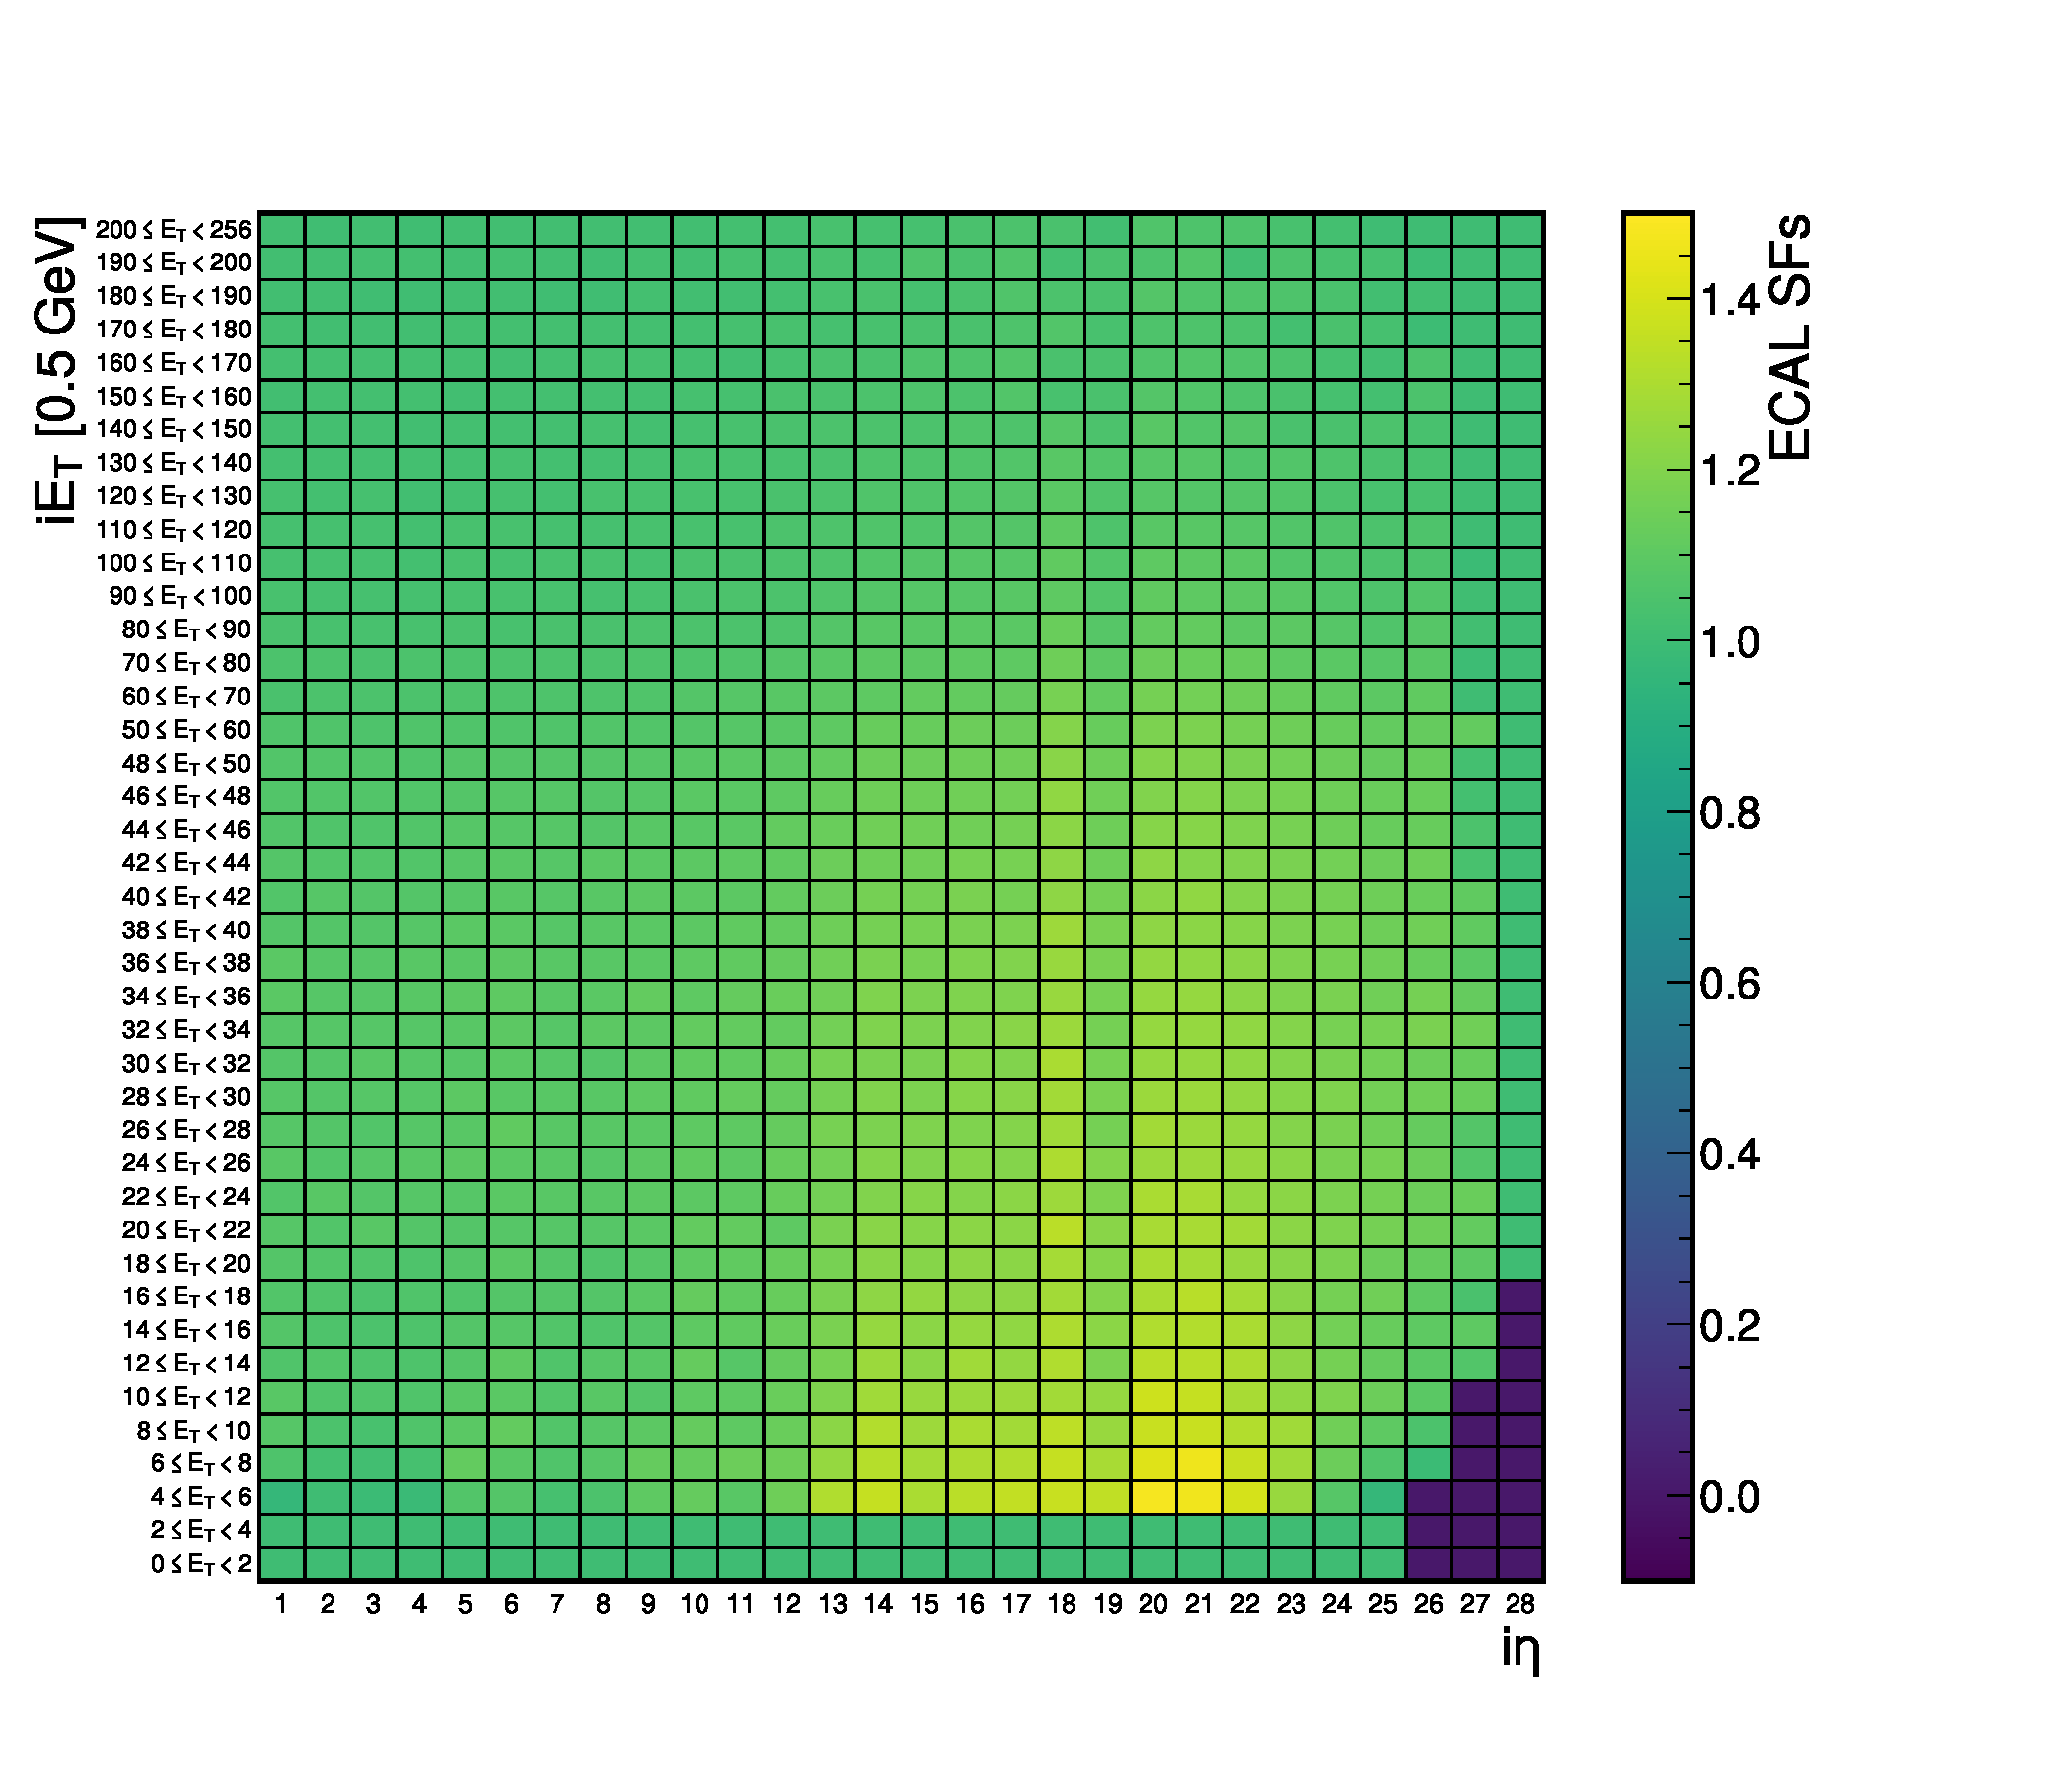
\includegraphics[width=0.5\linewidth]{Figures/L1TP/SFs_2D_ECAL_Thesis_JAX.pdf}}
    \subfloat[JAX method (HCAL)]{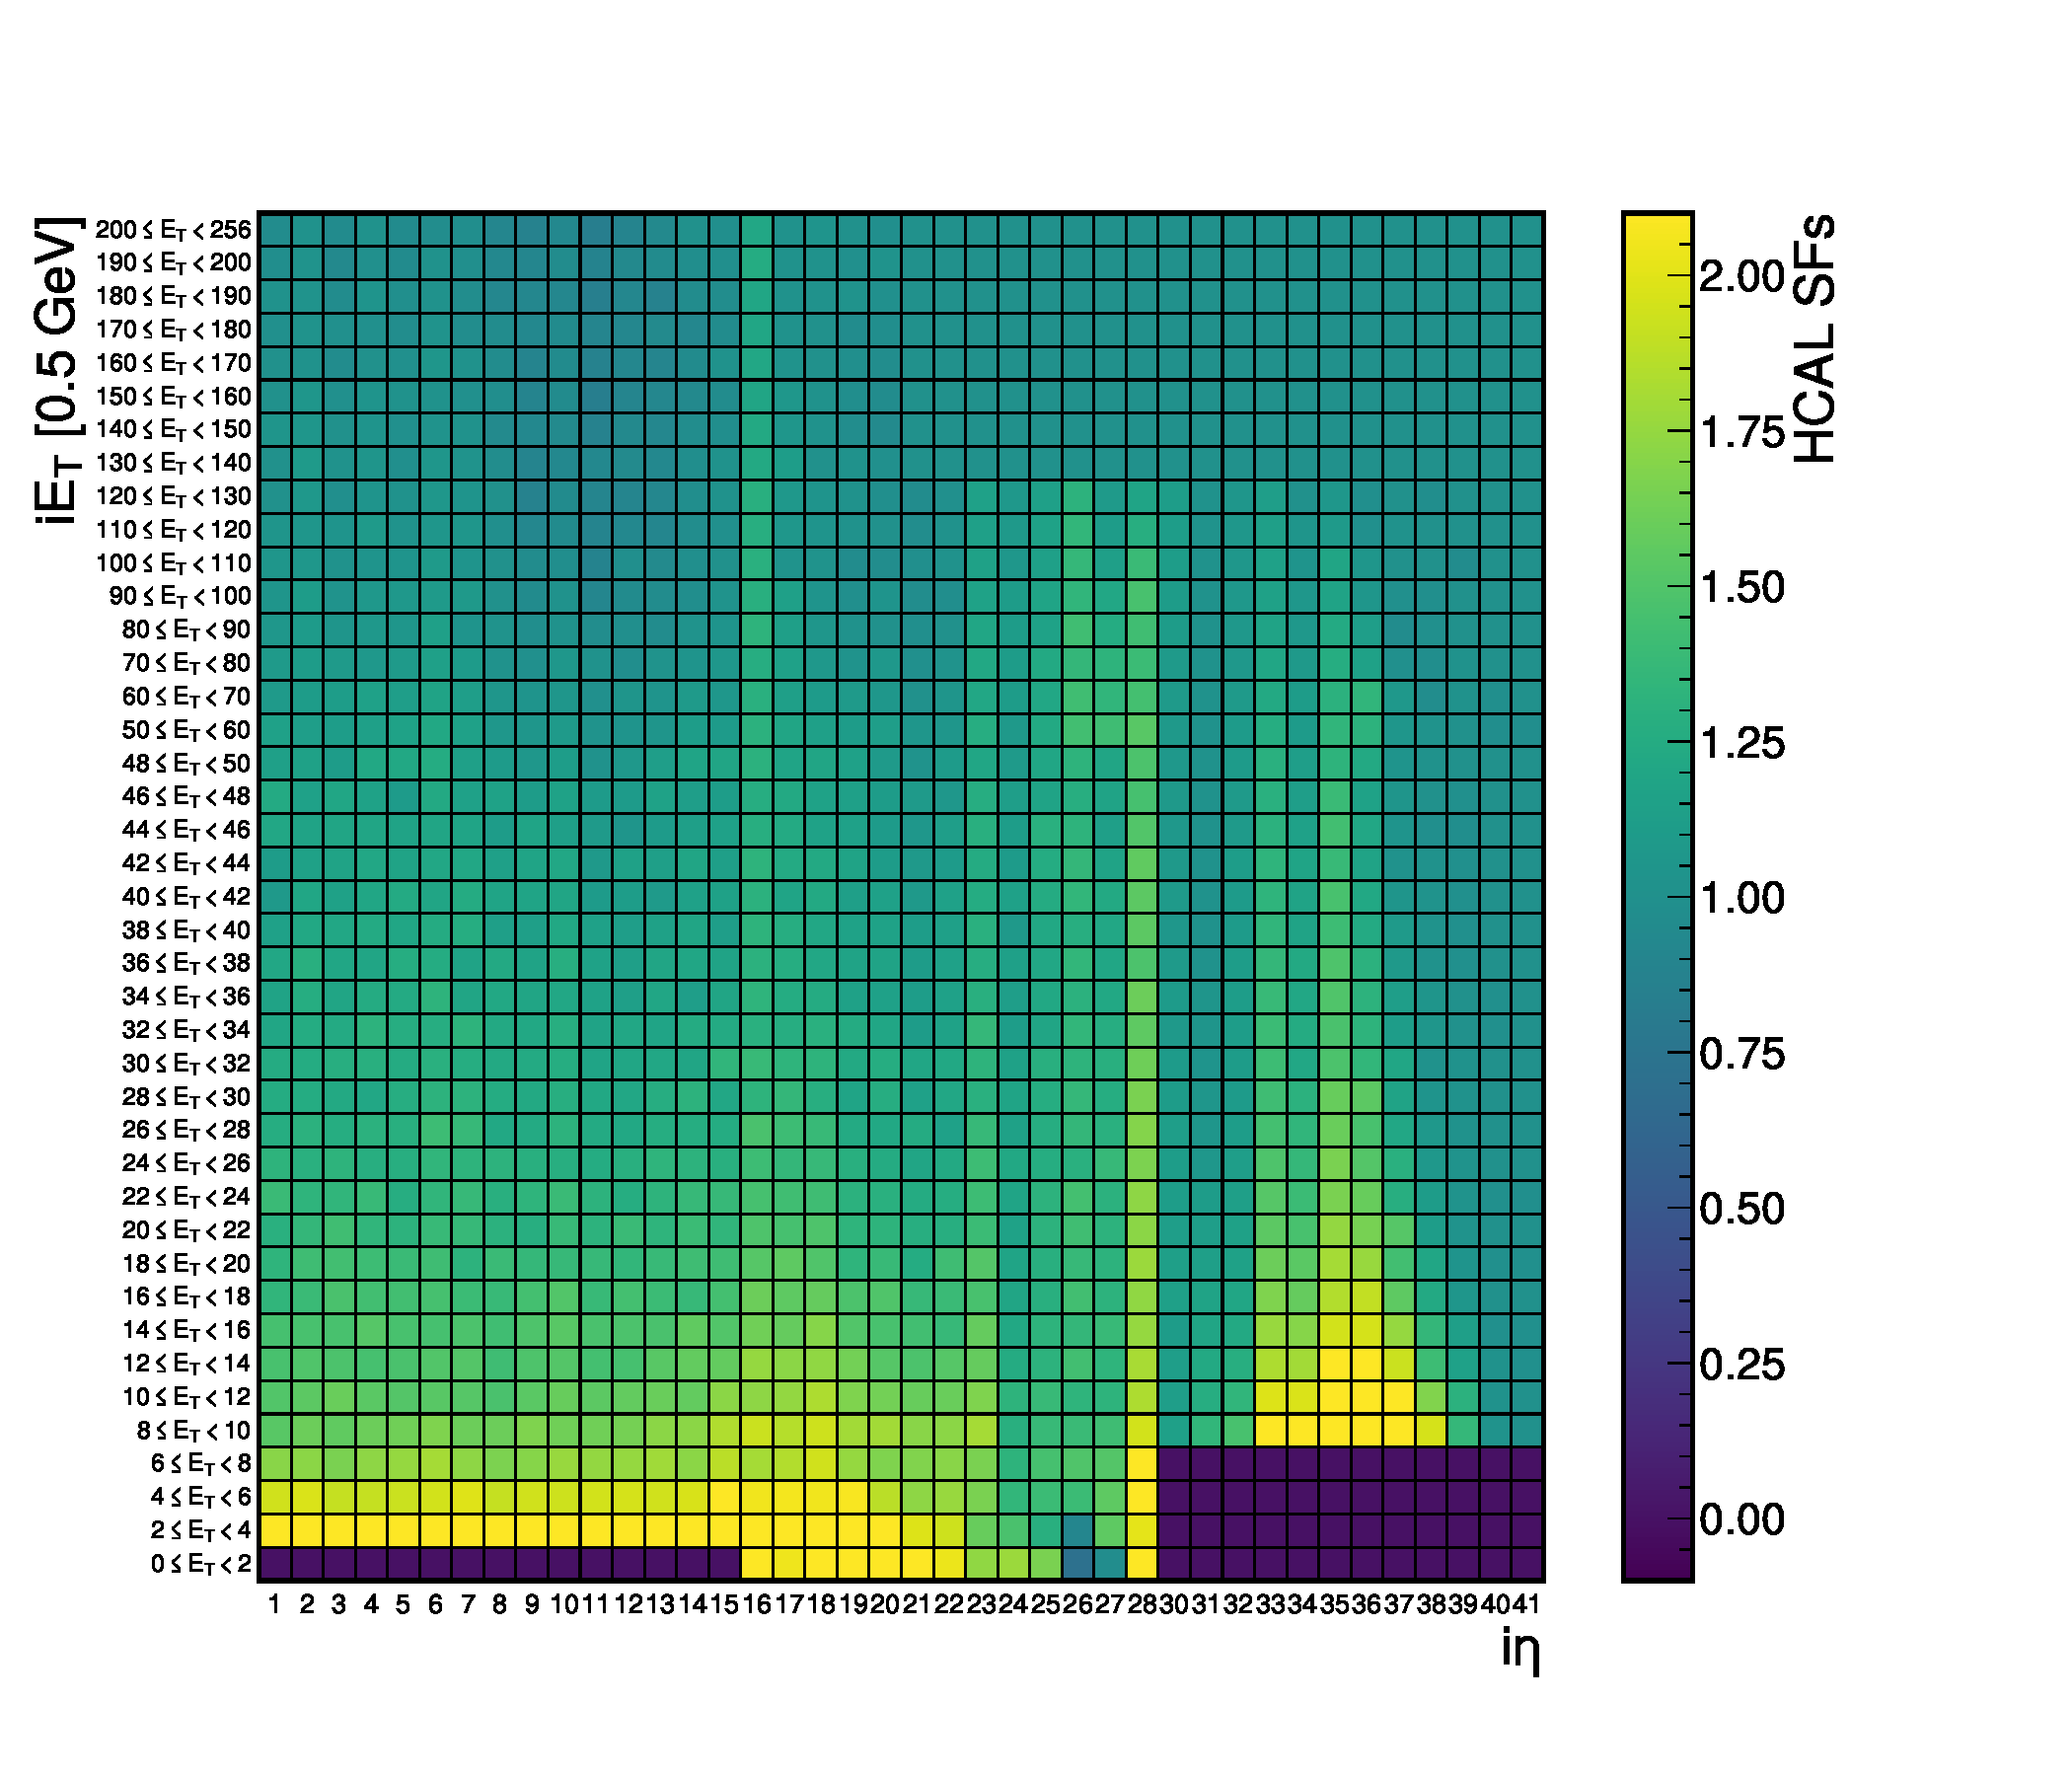
\includegraphics[width=0.5\linewidth]{Figures/L1TP/SFs_2D_HCAL_Thesis_JAX.pdf}}
    \caption{Layer-1 ECAL (a) and HCAL (b) calibration factors extracted through the JAX approach. The colour map represents the calibration factor value, lower (higher) for darker (brighter) shades. Each bin corresponds to a given $i\eta$ position and range of raw energy deposit, in $iE_T$ units (corresponding to 0.5~GeV). In the ECAL Layer-1 configuration, the default zero-suppression for $i\eta=26,27,28$ is applied; in addition, the calibration factors for the first two energy bins are constrained to 1, for the optimisation of the Layer-2 pile-up estimator. In the HCAL Layer-1 configuration, the JAX configuration applies the zero-suppression of TTs with $E_T=0.5$~GeV and $|i\eta|\leq15$ directly within the training procedure, allowing for the adjacent values to be adapted accordingly. In the HF region, a zero-suppression is also applied to all towers for $E_T<8$~GeV, expected to improvement the L1 jet performance.}
    \label{fig:JAX_SFs}
\end{figure}

In the case of ECAL, the calibration factors are confirmed to be close to unity, and the suppression of low-energy TTs in the barrel is cancelled by the constraint of the calibration factor values to 1. The discontinuity corresponding to $i\eta=18$, already observed in the current method and in the NN approach, is still present, confirming the capability of the JAX method to interpolate the same pattern even with a simpler architecture. 
An additional difference with respect to the NN approach is noticeable for $i\eta=28$, where the zero-suppression of low-energy TTs does not propagate to high energies.
The discreteness of the JAX method ensures independence between different energy bins, and avoids indiscriminate extrapolation of the detector response in regions covered by low statistics.

In the case of HCAL, the calibration factors generally show values larger than 1, with a strong increase towards lower-energy towers. 
The possibility of constraining the calibration factors in the barrel zero-suppression region allows the model to adapt the adjacent values accordingly, thus resulting in higher scale factors with respect to the NN results.
The pattern around the region $i\eta=17$ is still present, due to the reduced depth in HCAL crystals in the transition area between barrel and endcap. In addition, a new region is enhanced around position $i\eta=28$, corresponding to the transition between HCAL and HF. The difference with respect to the NN approach in this area is probably due to the fact that the NN has been trained for HCAL and HF separately, to allow for a better convergence of the model, while in the JAX training the two regions are trained simultaneously and allow for a better corrections in the transition area.
In HF, the zero-suppression of low energy TTs is visible in the first four energy bins, corresponding to energy $E_T<8$~GeV: this constraint has been required by Layer-2 jet experts, as it is expected to reduce the low-energy pile-up activity and improve jet performance in the high-pseudorapidity region. However, the training tends to compensate for the suppression at low-energy by enhancing the calibration factors for medium-energy towers in the region around $i\eta=35$.

\begin{figure}
    \centering
    \subfloat[Inclusive Response]{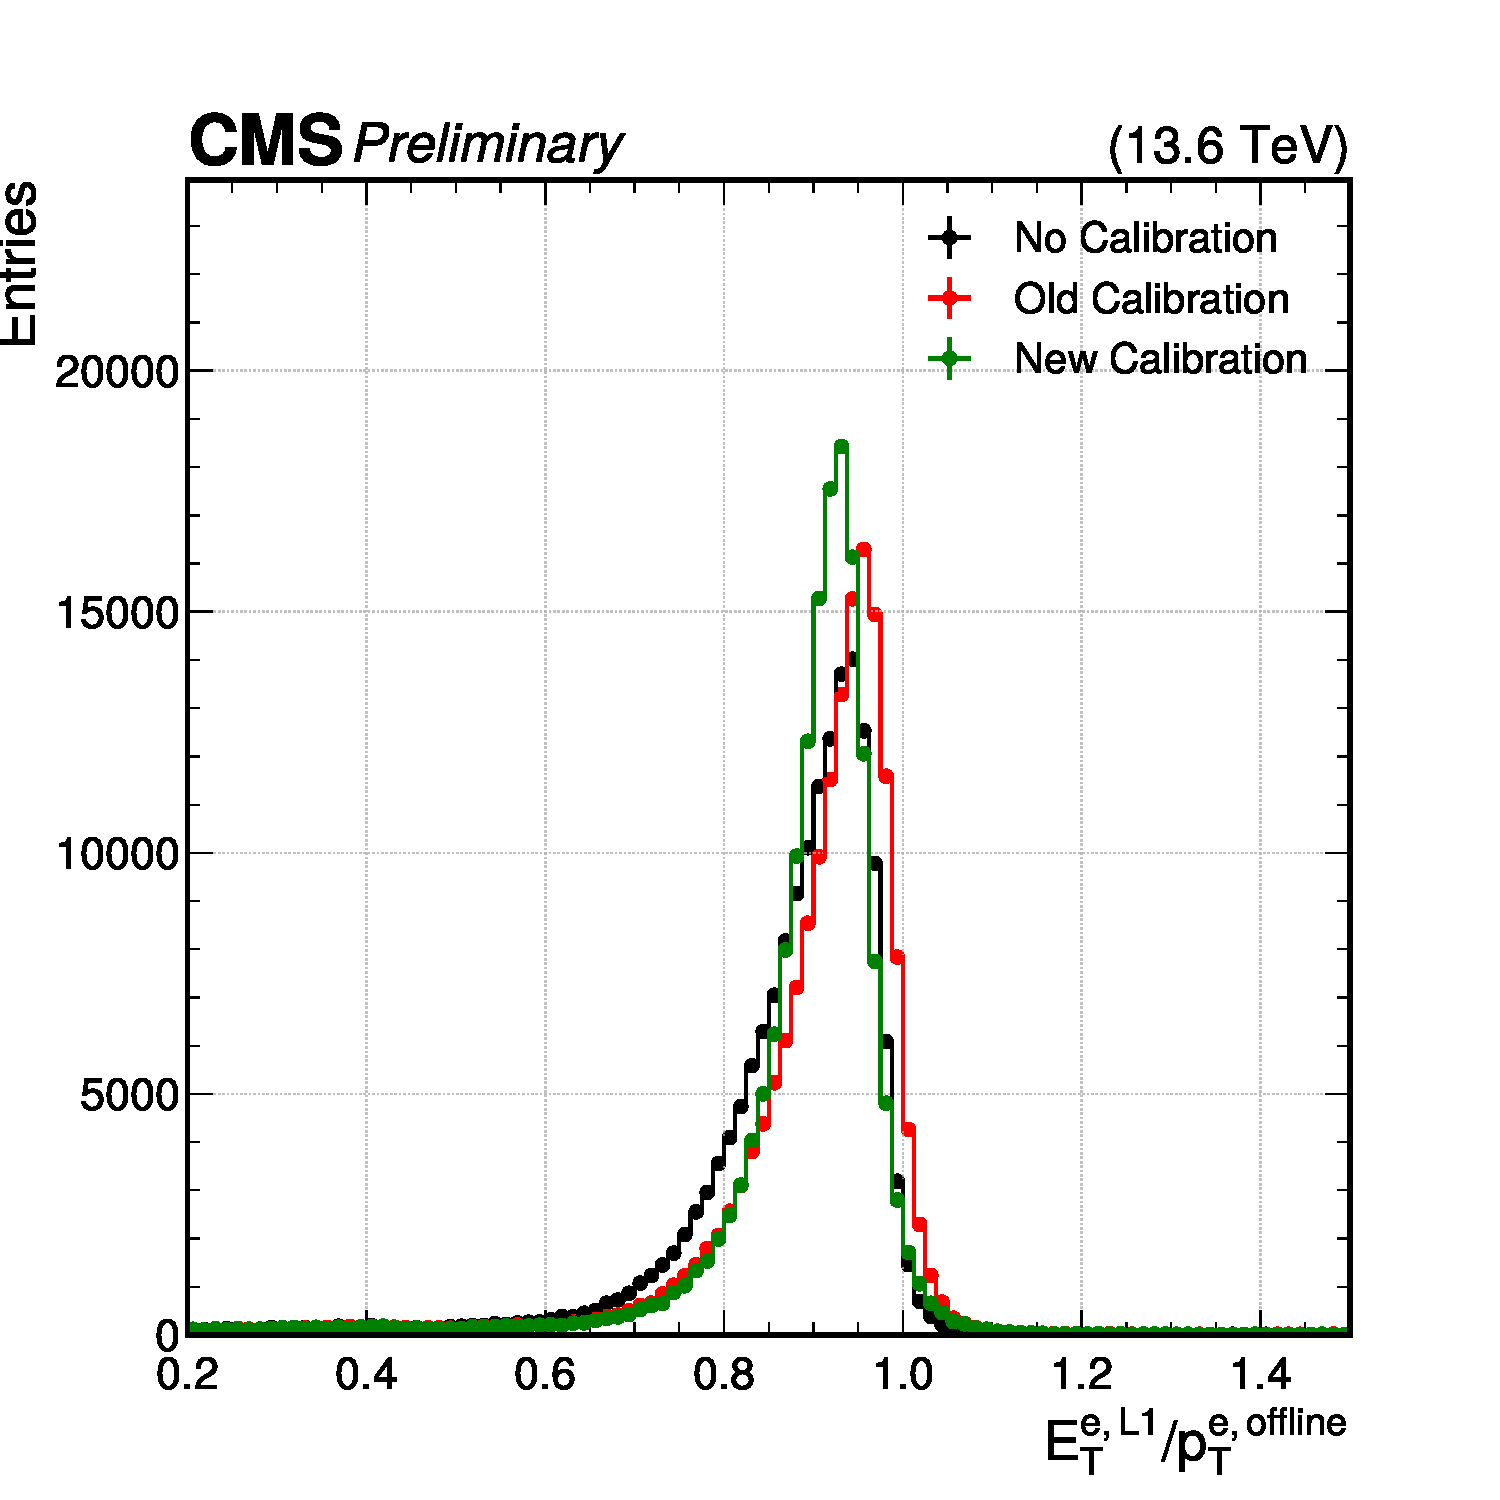
\includegraphics[width=0.5\linewidth]{Figures/L1TP/JAX_Performance/response_inclusive__ele.pdf}}
    
    \subfloat[Energy Resolution]{\includegraphics[width=0.5\linewidth]{Figures/L1TP/JAX_Performance/resolution_ptBins__ele.pdf}}
    \subfloat[Energy Scale]{\includegraphics[width=0.5\linewidth]{Figures/L1TP/JAX_Performance/scale_ptBins__ele.pdf}}
    \caption{Layer-1 $e/\gamma$ performance of the calibration factors derived through the JAX approach, in terms of energy response (a), energy resolution (b) and energy scale (c) as a function of the offline $p_T$. The energy of the L1 $e/\gamma$ candidate is obtained by replicating the Layer-1 firmware with three different configurations: no calibration (black), old calibration (red), and new JAX-based calibration (green); no Layer-2 calibration is applied to the L1 candidate.
}
    \label{fig:JAX_ECAL_Response}
\end{figure}

\begin{figure}
    \centering
    \subfloat[Rate]{\includegraphics[width=0.5\linewidth]{Figures/L1TP/JAX_Performance/rate_ObjEr2p5__ele.pdf}}
    
    \subfloat[Efficiency turn-on: $p_T>12$~GeV]{\includegraphics[width=0.5\linewidth]{Figures/L1TP/NN_Performance/turnon_fixedObjRateEr2p5_12__ele.pdf}}
    \subfloat[Efficiency turn-on: $p_T>36$~GeV]{\includegraphics[width=0.5\linewidth]{Figures/L1TP/JAX_Performance/turnon_fixedObjRateEr2p5_36__ele.pdf}}
    \caption{Layer-1 $e/\gamma$ performance of the calibration factors derived through the JAX approach, in terms of rate (a) and efficiency turn-on curves (b-c) for two fixed rate thresholds, to guarantee a fair comparison among different Layer-1 configurations. The energy of the L1 $e/\gamma$ candidate is obtained by replicating the Layer-1 firmware with three different configurations: no calibration (black), old calibration (red), and new JAX-based calibration (green); no Layer-2 calibration is applied to the L1 candidate.}
    \label{fig:JAX_ECAL_TurnOn}
\end{figure}

\begin{figure}
    \centering
    \subfloat[Inclusive Response]{\includegraphics[width=0.5\linewidth]{Figures/L1TP/JAX_Performance/response_inclusive__jet.pdf}}
    
    \subfloat[Energy Resolution]{\includegraphics[width=0.5\linewidth]{Figures/L1TP/JAX_Performance/resolution_ptBins__jet.pdf}}
    \subfloat[Energy Scale]{\includegraphics[width=0.5\linewidth]{Figures/L1TP/JAX_Performance/scale_ptBins__jet.pdf}}
    \caption{Layer-1 jet performance of the calibration factors derived through the JAX approach, in terms of energy response (a), energy resolution (b) and energy scale (c) as a function of the offline $p_T$. The energy of the L1 jet candidate is obtained by replicating the Layer-1 firmware with three different configurations: no calibration (black), old calibration (red), and new JAX-based calibration (green); no Layer-2 calibration is applied to the L1 candidate.}
    \label{fig:JAX_HCAL_Response}
\end{figure}

\begin{figure}
    \centering
    \subfloat[Rate $|\eta|<2.5$]{\includegraphics[width=0.5\linewidth]{Figures/L1TP/JAX_Performance/rate_ObjEr2p5__jet.pdf}}
    
    \subfloat[Efficiency turn-on $|\eta|<2.5$: $p_T>40$~GeV]{\includegraphics[width=0.5\linewidth]{Figures/L1TP/NN_Performance/turnon_fixedObjRateEr2p5_40__jet.pdf}}
    \subfloat[Efficiency turn-on $|\eta|<2.5$: $p_T>60$~GeV]{\includegraphics[width=0.5\linewidth]{Figures/L1TP/JAX_Performance/turnon_fixedObjRateEr2p5_60__jet.pdf}}
    \caption{Layer-1 jet performance of the calibration factors derived through the JAX approach, in terms of rate (a) and efficiency turn-on curves (b-c) for two fixed rate thresholds, to guarantee a fair comparison among different Layer-1 configurations. The energy of the L1 jet candidate is obtained by replicating the Layer-1 firmware with three different configurations: no calibration (black), old calibration (red), and new JAX-based calibration (green); no Layer-2 calibration is applied to the L1 candidate. The $|\eta|<2.5$ region is considered, since a vast number of jet trigger seeds only consider this pseudorapidity region.}
    \label{fig:JAX_HCAL_TurnOn_Er2p5}
\end{figure}

\begin{figure}
    \centering
    \subfloat[Rate]{\includegraphics[width=0.5\linewidth]{Figures/L1TP/JAX_Performance/rate_Obj__jet.pdf}}
    
    \subfloat[Efficiency turn-on: $p_T>60$~GeV]{\includegraphics[width=0.5\linewidth]{Figures/L1TP/NN_Performance/turnon_fixedObjRate_60__jet.pdf}}
    \subfloat[Efficiency turn-on: $p_T>80$~GeV]{\includegraphics[width=0.5\linewidth]{Figures/L1TP/JAX_Performance/turnon_fixedObjRate_80__jet.pdf}}
    \caption{Layer-1 jet performance of the calibration factors derived through the JAX approach, in terms of rate (a) and efficiency turn-on curves (b-c) for two fixed rate thresholds, to guarantee a fair comparison among different Layer-1 configurations. The energy of the L1 jet candidate is obtained by replicating the Layer-1 firmware with three different configurations: no calibration (black), old calibration (red), and new JAX-based calibration (green); no Layer-2 calibration is applied to the L1 candidate. The full pseudorapidity region is considered.}
    \label{fig:JAX_HCAL_TurnOn}
\end{figure}

\bigbreak

The performance of the new Layer-1 calibration factors derived through the JAX method is evaluated by replicating the Layer-1 firmware with the new LUT, following the same strategy used for the NN approach. A dataset collected by the CMS experiment during Run~III data taking is re-emulated under three different Layer-1 configurations: one in which no calibration is applied (No calibration), one in which the calibration factors are set to the values obtained with the old method (Old calibration), and one in which the calibration constants are derived with the JAX approach presented in this section (New calibration). 
The three configurations are compared in terms of Layer-1 energy response, scale and resolution, and of efficiency turn-on sharpness for fixed L1 rate thresholds. 

The Layer-1 performance on $e/\gamma$ candidates is presented in Figure~\ref{fig:JAX_ECAL_Response} and \ref{fig:JAX_ECAL_TurnOn}. The JAX approach provides better calibration of the ECAL TTs, resulting in better scale and resolution across the entire $p_T$ spectrum. The constrain on low-energy calibration factors leads to higher scale, and a slight rate increase; however, the better resolution is able to furnish sharper efficiency turn-on curves in the whole range of $p_T$ thresholds.

The resulting Layer-1 performance on jet candidates is shown in Figure~\ref{fig:JAX_HCAL_Response}, \ref{fig:JAX_HCAL_TurnOn_Er2p5} and \ref{fig:JAX_HCAL_TurnOn}.
The new JAX method provides better Layer-1 performance with respect to the NN-based calibration on jets: this result is due to a better calibration of HCAL towers, which are key for the construction of L1 jet candidates. The JAX-based HCAL calibration factors better integrate the zero-suppression configuration, and are able to better interpolate the detector pattern in the transition regions. The JAX approach leads to a better calibration of jet candidates at Layer-1, showing response distribution more centred towards unity, better scale and resolution across the entire $p_T$ range. 
The higher calibration factors cause a slight rate increase, nevertheless the better resolution leads to a sharper efficiency turn-on curve at fixed rate with respect to the old calibration, providing results at Layer-1 compatible with the NN-based approach.

\subsection{The Layer-2 validation} 

The JAX approach bla bla bla

\begin{figure}
    \centering
    \subfloat[]{\includegraphics[width=0.5\linewidth]{Figures/L1TP/JAX_Layer2_Taus.pdf}}
    \label{fig:JAX_Layer2_Taus}
\end{figure}

\section{Future applications} % 1/7

\section*{Summary} % 2/7 + introduction and revision
	% \chapter{The study of ZZ/ZH production in the $bb\tau\tau$ final state}

\section{The ZZ/ZH production as a validation for Di-Higgs searches}

\section{The ZZ/ZH production beyond the Standard Model}

\section{Physics objects pre-selection}
\subsection {Trigger requirements}
\subsection {Pre-selection of $Z/H \rightarrow \tau\tau$ objects}
\subsection {Pre-selection of $Z/H \rightarrow bb$ objects}

\section{Event selection and analysis flow}
\subsection{Definition of the signal region}
\subsection{Definition of the categories}
\subsection{Selection efficiency}
\subsection{Deep Neural Network for the signal extraction}

\section{Modelling of physics processes}
\subsection{Properties of Monte Carlo simulation}
\subsection{The Standard Model ZZ/ZH signal modelling}
\subsection{The resonant ZZ/ZH signal modelling}
\subsection{$t\bar{t}$ background modelling}
\subsection{Drell-Yan background modelling}
\subsection{Multi-jet background modelling}
\subsection{Other backgrounds modelling}

\section{Systematic uncertainties}
\subsection{Normalisation uncertainties}
\subsection{Shape uncertainties}
\subsection{Impact of systematic uncertainties}
	% \chapter{Statistical analysis and results on the ZZ/ZH production in the $bb\tau\tau$ final state}

\section{The final discriminant}

\section{Statistical interpretation}
\subsection{Expected signal strength for the Standard Model process}
\subsection{Expected upper limit for the resonant process}

\section{Results}
\subsection{Dataset analysed}
\subsection{The Standard Model interpretation}
\subsection{The resonant interpretation}

\section{Prospects for the ZZ/ZH analysis}


	% \chapter*{Conclusion}
\addcontentsline{toc}{chapter}{Conclusion}

        \bibliographystyle{unsrt} \bibliography{Bib.bib}
        % \begin{thebibliography}{1}

\bibitem{TDR}
The CMS Collaboration, The Phase-2 Upgrade of the CMS Endcap
Calorimeter, CERN-LHCC-2017-023, 2017.
\bibitem{ADC}
M. Firlej et al., A fast, ultra-low and frequency-scalable power consumption, 10-bit SAR ADC for particle physics detectors, JINST 10 P11012, 2015.
\bibitem{RAM1}
A. Marchioro et al., Design of power-efficient RAM memories for LHC Front-End chips, Contribution to the Front-End Electronics Conference, 2018.
\bibitem{perf1}
F. Bouyjou et al., HGCROC3 : the front-end readout ASIC for the CMS High Granularity Calorimeter, 2022 JINST 17 C03015.
\bibitem{perf2}
G. Bombardi et al., HGCROC-Si and HGCROC-SiPM : the front- end readout ASICs for the CMS HGCAL, 2020, IEEE Nuclear Science Symposium and Medical Imaging Conference, doi: 10.1109/NSS/MIC42677.2020.9508012
\bibitem{fluka}
A. Fassò, A. Ferrari, J. Ranft, P. Sala, in: A. Menzione, A. Scribano (Eds.), Proceedings of the IV International Conference on Calorimetry in High Energy Physics, La Biodola, Sept. 20-25, 1993., World Scientific, Singapore, 1993, p. 493.
\bibitem{giulio}
G. Borghello et al., "Dose-Rate Sensitivity of 65-nm MOSFETs Exposed to Ultrahigh Doses," in IEEE Transactions on Nuclear Science, vol. 65, no. 8, pp. 1482-1487, Aug. 2018, doi: 10.1109/TNS.2018.2828142. % https://ieeexplore.ieee.org/document/8340851
\bibitem{federico}
M. Huhtinen, F. Faccio, "Computational method to estimate single event upset rates in an accelerator environment", in Nucl. Instrum. Meth. A, 2000, doi: 10.1016/S0168-9002(00)00155-8.
\bibitem{currentL1}
The CMS Collaboration, Performance of the CMS Level-1 trigger in proton-proton collisions at $\sqrt{s}=13\;TeV$, JINST 15 P10017, 2020.
\bibitem{SM}
M. J. Herrero, "The Srandard Model". arXiv:hep-ph/9812242
\bibitem{discovery1}
The ATLAS Collaboration, “Observation of a new particle in the search for the standard model Higgs boson with the ATLAS detector at the LHC”, Phys. Lett. B 716 (2012) 1, doi:10.1016/j.physletb.2012.08.020, arXiv:1207.7214.
\bibitem{discovery2}
The CMS Collaboration, “Observation of a new boson at a mass of 125 GeV with the CMS experiment at the LHC”, Phys. Lett. B 716 (2012) 30, doi:10.1016/j.physletb.2012.08.021, arXiv:1207.7235.
\bibitem{discovery3}
The CMS collaboration, Chatrchyan, S., Khachatryan, V. et al. Observation of a new boson with mass near 125 GeV in pp collisions at $\sqrt{s}$ = 7 and 8 TeV. J. High Energ. Phys. 2013, 81 (2013), doi:10.1007/JHEP06(2013)081
\bibitem{mh}
The ATLAS anc CMS collaborations, "Combined Measurement of the Higgs Boson Mass in pp Collisions at $\sqrt{s}$ = 7 and 8 TeV with the ATLAS and CMS Experiments". Phys. Rev. Lett. 114 (2015) 191803, doi:10.1103/PhysRevLett.114.191803, arXiv:1503.07589.
\bibitem{Hproperties}
The ATLAS anc CMS collaborations, "Measurements of the Higgs boson production and decay rates and constraints on its couplings from a combined ATLAS and CMS analysis of the LHC pp collision data at $\sqrt{s}$ = 7 and 8 TeV". JHEP 08 (2016) 045, 
doi:10.48550/arXiv.1606.02266.
\bibitem{paperbbtautau}
The CMS collaboration, "Search for nonresonant Higgs boson pair production in final state with two bottom quarks and two tau leptons in proton-proton collisions at $\sqrt{s}$ = 13 TeV". Phys. Lett. B 842 (2023) 137531, arXiv:2206.09401, 
doi:10.1016/j.physletb.2022.137531.

\end{thebibliography}
        % \begin{thebibliography}{1}

\bibitem{TDR}
The CMS Collaboration, The Phase-2 Upgrade of the CMS Endcap
Calorimeter, CERN-LHCC-2017-023, 2017.
\bibitem{ADC}
M. Firlej et al., A fast, ultra-low and frequency-scalable power consumption, 10-bit SAR ADC for particle physics detectors, JINST 10 P11012, 2015.
\bibitem{RAM1}
A. Marchioro et al., Design of power-efficient RAM memories for LHC Front-End chips, Contribution to the Front-End Electronics Conference, 2018.
\bibitem{perf1}
F. Bouyjou et al., HGCROC3 : the front-end readout ASIC for the CMS High Granularity Calorimeter, 2022 JINST 17 C03015.
\bibitem{perf2}
G. Bombardi et al., HGCROC-Si and HGCROC-SiPM : the front- end readout ASICs for the CMS HGCAL, 2020, IEEE Nuclear Science Symposium and Medical Imaging Conference, doi: 10.1109/NSS/MIC42677.2020.9508012
\bibitem{fluka}
A. Fassò, A. Ferrari, J. Ranft, P. Sala, in: A. Menzione, A. Scribano (Eds.), Proceedings of the IV International Conference on Calorimetry in High Energy Physics, La Biodola, Sept. 20-25, 1993., World Scientific, Singapore, 1993, p. 493.
\bibitem{giulio}
G. Borghello et al., "Dose-Rate Sensitivity of 65-nm MOSFETs Exposed to Ultrahigh Doses," in IEEE Transactions on Nuclear Science, vol. 65, no. 8, pp. 1482-1487, Aug. 2018, doi: 10.1109/TNS.2018.2828142. % https://ieeexplore.ieee.org/document/8340851
\bibitem{federico}
M. Huhtinen, F. Faccio, "Computational method to estimate single event upset rates in an accelerator environment", in Nucl. Instrum. Meth. A, 2000, doi: 10.1016/S0168-9002(00)00155-8.
\bibitem{currentL1}
The CMS Collaboration, Performance of the CMS Level-1 trigger in proton-proton collisions at $\sqrt{s}=13\;TeV$, JINST 15 P10017, 2020.
\bibitem{SM}
M. J. Herrero, "The Srandard Model". arXiv:hep-ph/9812242
\bibitem{discovery1}
The ATLAS Collaboration, “Observation of a new particle in the search for the standard model Higgs boson with the ATLAS detector at the LHC”, Phys. Lett. B 716 (2012) 1, doi:10.1016/j.physletb.2012.08.020, arXiv:1207.7214.
\bibitem{discovery2}
The CMS Collaboration, “Observation of a new boson at a mass of 125 GeV with the CMS experiment at the LHC”, Phys. Lett. B 716 (2012) 30, doi:10.1016/j.physletb.2012.08.021, arXiv:1207.7235.
\bibitem{discovery3}
The CMS collaboration, Chatrchyan, S., Khachatryan, V. et al. Observation of a new boson with mass near 125 GeV in pp collisions at $\sqrt{s}$ = 7 and 8 TeV. J. High Energ. Phys. 2013, 81 (2013), doi:10.1007/JHEP06(2013)081
\bibitem{mh}
The ATLAS anc CMS collaborations, "Combined Measurement of the Higgs Boson Mass in pp Collisions at $\sqrt{s}$ = 7 and 8 TeV with the ATLAS and CMS Experiments". Phys. Rev. Lett. 114 (2015) 191803, doi:10.1103/PhysRevLett.114.191803, arXiv:1503.07589.
\bibitem{Hproperties}
The ATLAS anc CMS collaborations, "Measurements of the Higgs boson production and decay rates and constraints on its couplings from a combined ATLAS and CMS analysis of the LHC pp collision data at $\sqrt{s}$ = 7 and 8 TeV". JHEP 08 (2016) 045, 
doi:10.48550/arXiv.1606.02266.
\bibitem{paperbbtautau}
The CMS collaboration, "Search for nonresonant Higgs boson pair production in final state with two bottom quarks and two tau leptons in proton-proton collisions at $\sqrt{s}$ = 13 TeV". Phys. Lett. B 842 (2023) 137531, arXiv:2206.09401, 
doi:10.1016/j.physletb.2022.137531.

\end{thebibliography}

\end{document}